% Options for packages loaded elsewhere
\PassOptionsToPackage{unicode}{hyperref}
\PassOptionsToPackage{hyphens}{url}
%
\documentclass[
]{book}
\usepackage{lmodern}
\usepackage{amssymb,amsmath}
\usepackage{ifxetex,ifluatex}
\ifnum 0\ifxetex 1\fi\ifluatex 1\fi=0 % if pdftex
  \usepackage[T1]{fontenc}
  \usepackage[utf8]{inputenc}
  \usepackage{textcomp} % provide euro and other symbols
\else % if luatex or xetex
  \usepackage{unicode-math}
  \defaultfontfeatures{Scale=MatchLowercase}
  \defaultfontfeatures[\rmfamily]{Ligatures=TeX,Scale=1}
\fi
% Use upquote if available, for straight quotes in verbatim environments
\IfFileExists{upquote.sty}{\usepackage{upquote}}{}
\IfFileExists{microtype.sty}{% use microtype if available
  \usepackage[]{microtype}
  \UseMicrotypeSet[protrusion]{basicmath} % disable protrusion for tt fonts
}{}
\makeatletter
\@ifundefined{KOMAClassName}{% if non-KOMA class
  \IfFileExists{parskip.sty}{%
    \usepackage{parskip}
  }{% else
    \setlength{\parindent}{0pt}
    \setlength{\parskip}{6pt plus 2pt minus 1pt}}
}{% if KOMA class
  \KOMAoptions{parskip=half}}
\makeatother
\usepackage{xcolor}
\IfFileExists{xurl.sty}{\usepackage{xurl}}{} % add URL line breaks if available
\IfFileExists{bookmark.sty}{\usepackage{bookmark}}{\usepackage{hyperref}}
\hypersetup{
  pdftitle={The RJafroc Quick Start Book},
  pdfauthor={Dev P. Chakraborty, PhD},
  hidelinks,
  pdfcreator={LaTeX via pandoc}}
\urlstyle{same} % disable monospaced font for URLs
\usepackage{color}
\usepackage{fancyvrb}
\newcommand{\VerbBar}{|}
\newcommand{\VERB}{\Verb[commandchars=\\\{\}]}
\DefineVerbatimEnvironment{Highlighting}{Verbatim}{commandchars=\\\{\}}
% Add ',fontsize=\small' for more characters per line
\usepackage{framed}
\definecolor{shadecolor}{RGB}{248,248,248}
\newenvironment{Shaded}{\begin{snugshade}}{\end{snugshade}}
\newcommand{\AlertTok}[1]{\textcolor[rgb]{0.94,0.16,0.16}{#1}}
\newcommand{\AnnotationTok}[1]{\textcolor[rgb]{0.56,0.35,0.01}{\textbf{\textit{#1}}}}
\newcommand{\AttributeTok}[1]{\textcolor[rgb]{0.77,0.63,0.00}{#1}}
\newcommand{\BaseNTok}[1]{\textcolor[rgb]{0.00,0.00,0.81}{#1}}
\newcommand{\BuiltInTok}[1]{#1}
\newcommand{\CharTok}[1]{\textcolor[rgb]{0.31,0.60,0.02}{#1}}
\newcommand{\CommentTok}[1]{\textcolor[rgb]{0.56,0.35,0.01}{\textit{#1}}}
\newcommand{\CommentVarTok}[1]{\textcolor[rgb]{0.56,0.35,0.01}{\textbf{\textit{#1}}}}
\newcommand{\ConstantTok}[1]{\textcolor[rgb]{0.00,0.00,0.00}{#1}}
\newcommand{\ControlFlowTok}[1]{\textcolor[rgb]{0.13,0.29,0.53}{\textbf{#1}}}
\newcommand{\DataTypeTok}[1]{\textcolor[rgb]{0.13,0.29,0.53}{#1}}
\newcommand{\DecValTok}[1]{\textcolor[rgb]{0.00,0.00,0.81}{#1}}
\newcommand{\DocumentationTok}[1]{\textcolor[rgb]{0.56,0.35,0.01}{\textbf{\textit{#1}}}}
\newcommand{\ErrorTok}[1]{\textcolor[rgb]{0.64,0.00,0.00}{\textbf{#1}}}
\newcommand{\ExtensionTok}[1]{#1}
\newcommand{\FloatTok}[1]{\textcolor[rgb]{0.00,0.00,0.81}{#1}}
\newcommand{\FunctionTok}[1]{\textcolor[rgb]{0.00,0.00,0.00}{#1}}
\newcommand{\ImportTok}[1]{#1}
\newcommand{\InformationTok}[1]{\textcolor[rgb]{0.56,0.35,0.01}{\textbf{\textit{#1}}}}
\newcommand{\KeywordTok}[1]{\textcolor[rgb]{0.13,0.29,0.53}{\textbf{#1}}}
\newcommand{\NormalTok}[1]{#1}
\newcommand{\OperatorTok}[1]{\textcolor[rgb]{0.81,0.36,0.00}{\textbf{#1}}}
\newcommand{\OtherTok}[1]{\textcolor[rgb]{0.56,0.35,0.01}{#1}}
\newcommand{\PreprocessorTok}[1]{\textcolor[rgb]{0.56,0.35,0.01}{\textit{#1}}}
\newcommand{\RegionMarkerTok}[1]{#1}
\newcommand{\SpecialCharTok}[1]{\textcolor[rgb]{0.00,0.00,0.00}{#1}}
\newcommand{\SpecialStringTok}[1]{\textcolor[rgb]{0.31,0.60,0.02}{#1}}
\newcommand{\StringTok}[1]{\textcolor[rgb]{0.31,0.60,0.02}{#1}}
\newcommand{\VariableTok}[1]{\textcolor[rgb]{0.00,0.00,0.00}{#1}}
\newcommand{\VerbatimStringTok}[1]{\textcolor[rgb]{0.31,0.60,0.02}{#1}}
\newcommand{\WarningTok}[1]{\textcolor[rgb]{0.56,0.35,0.01}{\textbf{\textit{#1}}}}
\usepackage{longtable,booktabs}
% Correct order of tables after \paragraph or \subparagraph
\usepackage{etoolbox}
\makeatletter
\patchcmd\longtable{\par}{\if@noskipsec\mbox{}\fi\par}{}{}
\makeatother
% Allow footnotes in longtable head/foot
\IfFileExists{footnotehyper.sty}{\usepackage{footnotehyper}}{\usepackage{footnote}}
\makesavenoteenv{longtable}
\usepackage{graphicx,grffile}
\makeatletter
\def\maxwidth{\ifdim\Gin@nat@width>\linewidth\linewidth\else\Gin@nat@width\fi}
\def\maxheight{\ifdim\Gin@nat@height>\textheight\textheight\else\Gin@nat@height\fi}
\makeatother
% Scale images if necessary, so that they will not overflow the page
% margins by default, and it is still possible to overwrite the defaults
% using explicit options in \includegraphics[width, height, ...]{}
\setkeys{Gin}{width=\maxwidth,height=\maxheight,keepaspectratio}
% Set default figure placement to htbp
\makeatletter
\def\fps@figure{htbp}
\makeatother
\setlength{\emergencystretch}{3em} % prevent overfull lines
\providecommand{\tightlist}{%
  \setlength{\itemsep}{0pt}\setlength{\parskip}{0pt}}
\setcounter{secnumdepth}{5}
\usepackage{booktabs}
\usepackage{amsthm}
\makeatletter
\def\thm@space@setup{%
  \thm@preskip=8pt plus 2pt minus 4pt
  \thm@postskip=\thm@preskip
}
\makeatother
\usepackage{booktabs}
\usepackage{longtable}
\usepackage{array}
\usepackage{multirow}
\usepackage{wrapfig}
\usepackage{float}
\usepackage{colortbl}
\usepackage{pdflscape}
\usepackage{tabu}
\usepackage{threeparttable}
\usepackage{threeparttablex}
\usepackage[normalem]{ulem}
\usepackage{makecell}
\usepackage{xcolor}
\usepackage[]{natbib}
\bibliographystyle{apalike}

\title{The RJafroc Quick Start Book}
\author{Dev P. Chakraborty, PhD}
\date{2022-09-29}

\begin{document}
\maketitle

{
\setcounter{tocdepth}{1}
\tableofcontents
}
\hypertarget{preface}{%
\chapter*{Preface}\label{preface}}
\addcontentsline{toc}{chapter}{Preface}

\begin{itemize}
\tightlist
\item
  This online book is for those already somewhat familiar running Windows JAFROC to analyze data.
\item
  The Windows program has been replaced by \texttt{RJafroc}.
\item
  This book dives into how to use \texttt{RJafroc} to analyze ROC/FROC data.
\item
  It starts with explanation of the dataset structures for ROC and FROC studies.
\item
  This is followed by an explanation of DBM and OR analyses.
\end{itemize}

\hypertarget{rationale-and-organization}{%
\section{Rationale and Organization}\label{rationale-and-organization}}

\begin{itemize}
\tightlist
\item
  Intended as an online update to my print book \citep{chakraborty2017observer}.
\item
  All references in this book to \texttt{RJafroc} refer to the R package with that name (case sensitive) \citep{R-RJafroc}.
\item
  Since its publication in 2017 \texttt{RJafroc}, on which the \texttt{R} code examples in the print book depend, has evolved considerably causing many of the examples to ``break'' if one uses the most current version of \texttt{RJafroc}. The code will still run if one uses \href{https://cran.r-project.org/src/contrib/Archive/RJafroc/}{\texttt{RJafroc} 0.0.1} but this is inconvenient and misses out on many of the software improvements made since the print book appeared.
\item
  This gives me the opportunity to update the print book.
\item
  The online book has been divided into 3 books.

  \begin{itemize}
  \tightlist
  \item
    \textbf{This book:} \href{https://dpc10ster.github.io/RJafrocQuickStart/}{RJafrocQuickStartBook}.
  \item
    The \href{https://dpc10ster.github.io/RJafrocRocBook/}{RJafrocRocBook} book.
  \item
    The \href{https://dpc10ster.github.io/RJafrocFrocBook/}{RJafrocFrocBook}.
  \end{itemize}
\end{itemize}

\hypertarget{tba-acknowledgements}{%
\section{TBA Acknowledgements}\label{tba-acknowledgements}}

Dr.~Xuetong Zhai

Dr.~Peter Phillips

Online Latex Editor \href{https://latexeditor.lagrida.com/}{at}

Dataset contributors

\hypertarget{part-quick-start}{%
\part*{Quick Start}\label{part-quick-start}}
\addcontentsline{toc}{part}{Quick Start}

\hypertarget{quick-start-help}{%
\chapter{Help}\label{quick-start-help}}

\hypertarget{quick-start-help-how-much-finished}{%
\section{TBA How much finished}\label{quick-start-help-how-much-finished}}

40\% (need to add images for one reader; add one-modality dataset)

\hypertarget{quick-start-help-getting-help}{%
\section{Getting help on the software}\label{quick-start-help-getting-help}}

\begin{itemize}
\tightlist
\item
  If you have installed \texttt{RJafroc} from \texttt{GitHub}:

  \begin{itemize}
  \tightlist
  \item
    ?\texttt{RJafroc-package} (RStudio will auto complete \ldots)
  \item
    Scroll down all the way and click on \texttt{Index}
  \end{itemize}
\item
  Regardless of where you installed from use the \texttt{RJafroc} help site:

  \begin{itemize}
  \tightlist
  \item
    \href{https://dpc10ster.github.io/RJafroc/}{RJafroc help site}
  \item
    Look under \texttt{References}
  \item
    For example, for help on the function \texttt{PlotEmpiricalOperatingCharacteristics}:
  \item
    \href{https://dpc10ster.github.io/RJafroc/reference/PlotEmpiricalOperatingCharacteristics.html}{PlotEmpiricalOperatingCharacteristics}
  \end{itemize}
\end{itemize}

\hypertarget{quick-start-help-references}{%
\section{References}\label{quick-start-help-references}}

\hypertarget{quick-start-data-format}{%
\chapter{JAFROC ROC data format}\label{quick-start-data-format}}

\hypertarget{quick-start-data-format-how-much-finished}{%
\section{TBA How much finished}\label{quick-start-data-format-how-much-finished}}

80\% (need to add images for one reader; add one-modality dataset)

\hypertarget{quick-start-data-format-intro}{%
\section{Introduction}\label{quick-start-data-format-intro}}

\begin{itemize}
\tightlist
\item
  JAFROC data format is named after the file format adopted circa. 2006 for the input Excel file to Windows JAFROC software.
\item
  The purpose of this chapter is to explain the data format of this file.
\item
  Reading this file into a dataset object suitable for \texttt{RJafroc} analysis is the subject of the next chapter.
\item
  Background on observer performance methods are in my book \citep{chakraborty2017observer}.
\item
  I will start with Receiver Operating Characteristic (ROC) data \citep{metz1978rocmethodology} as this is by far the simplest paradigm.
\item
  In the ROC paradigm the observer assigns a rating to each image. A rating is an ordered numeric label, and, in our convention, higher values represent greater certainty or \textbf{confidence level} for presence of disease. With human observers, a 5 (or 6) point rating scale is typically used, with 1 representing highest confidence for \emph{absence} of disease and 5 (or 6) representing highest confidence for \emph{presence} of disease. Intermediate values represent intermediate confidence levels for presence or absence of disease.
\item
  Note that location information, if applicable, associated with the disease, is not collected.
\item
  There is no restriction to 5 or 6 ratings. With algorithmic observers, e.g., computer aided detection (CAD) algorithms, the rating could be a floating point number and have infinite precision. All that is required is that higher values correspond to greater confidence in presence of disease.
\item
  The above is termed a \emph{positive-directed} rating scale. If lower numbers correspond to greater confidence, termed a negative-directed rating scale, a simple transformation to \(max(rating) - rating + 1\), where \(max(rating)\) is the maximum rating, over all readers, modalities and cases, will convert a negative-directed rating scale to a positive directed rating scale.
\end{itemize}

\hypertarget{quick-start-data-format-note-to-existing-users}{%
\section{Note to existing users}\label{quick-start-data-format-note-to-existing-users}}

\begin{itemize}
\tightlist
\item
  The Excel file format has recently undergone changes, involving three additional columns in the \texttt{Truth} worksheet.
\item
  \texttt{RJafroc} will work with old format Excel files as the additional columns are ignored.
\item
  Reasons for the change will become clearer in later chapters \footnote{They are needed for generalization to other data collection paradigms and for better data entry error control}.
\end{itemize}

\hypertarget{quick-start-data-format-contents}{%
\section{Contents of Excel file}\label{quick-start-data-format-contents}}

\begin{itemize}
\tightlist
\item
  The illustrations in this chapter correspond to Excel file \texttt{R/quick-start/rocCr.xlsx} in the project directory \footnote{To access files one needs to \texttt{fork} the repository, which creates, on your computer, a copy of all files used to create this document}. This is termed a \emph{toy file}, i.e., an artificial small dataset created to illustrate essential features of the data format.
\item
  The Excel file has three worksheets: \texttt{Truth}, \texttt{NL} (or \texttt{FP}) and \texttt{LL} (or \texttt{TP}).
\end{itemize}

\hypertarget{quick-start-data-format-truth-worksheet}{%
\section{\texorpdfstring{The \texttt{Truth} worksheet}{The Truth worksheet}}\label{quick-start-data-format-truth-worksheet}}

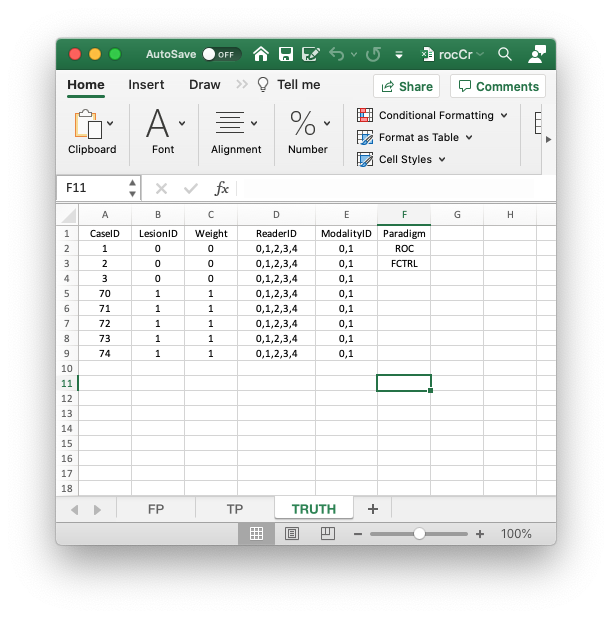
\includegraphics[width=1\textwidth,height=\textheight]{images/quick-start/rocCrTruth.png}

\begin{itemize}
\tightlist
\item
  The \texttt{Truth} worksheet contains 6 columns: \texttt{CaseID}, \texttt{LesionID}, \texttt{Weight}, \texttt{ReaderID}, \texttt{ModalityID} and \texttt{Paradigm}.
\item
  The first five columns contain as many rows as there are cases (images) in the dataset.
\item
  \texttt{CaseID}: \textbf{unique integers}, one per case, representing the cases in the dataset.
\item
  \texttt{LesionID}: integers 0 or 1, with each 0 representing a non-diseased case and each 1 representing a diseased case.
\item
  In the current dataset, the non-diseased cases are labeled \texttt{1}, \texttt{2} and \texttt{3}, while the diseased cases are labeled \texttt{70}, \texttt{71}, \texttt{72}, \texttt{73} and \texttt{74}. The values do not have to be consecutive integers; they need not be ordered; the only requirement is that they be \textbf{unique integers}.
\item
  \texttt{Weight}: A floating point value, typically filled in with 0 or 1; this field is not used for ROC data.
\item
  \texttt{ReaderID}: a \textbf{comma-separated} listing of reader labels, each represented by a \textbf{unique integer}, that have interpreted the case. In the example shown below each cell has the value \texttt{0,\ 1,\ 2,\ 3,\ 4} meaning that each of these readers has interpreted all cases (hence the ``factorial'' design).

  \begin{itemize}
  \tightlist
  \item
    \textbf{With multiple readers each cell in this column has to be text formatted as otherwise Excel will not accept it.}
  \item
    Select the worksheet, then \texttt{Format} - \texttt{Cells} - \texttt{Number} - \texttt{Text} - \texttt{OK}.
  \end{itemize}
\item
  \texttt{ModalityID}: a comma-separated listing of modalities, each represented by a \textbf{unique integer}, that are applied to each case. In the example each cell has the value \texttt{0,\ 1}.

  \begin{itemize}
  \tightlist
  \item
    \textbf{With multiple modalities each cell has to be text formatted as otherwise Excel will not accept it.}
  \item
    Format the cells as described above.
  \end{itemize}
\item
  \texttt{Paradigm}: this column contains two cells, \texttt{ROC} and \texttt{factorial}. It informs the software that this is an ROC dataset, and the design is factorial, meaning each reader has interpreted each case in each modality.
\item
  There are 5 diseased cases in the dataset (the number of 1's in the \texttt{LesionID} column of the \texttt{Truth} worksheet).
\item
  There are 3 non-diseased cases in the dataset (the number of 0's in the \texttt{LesionID} column).
\item
  There are 5 readers in the dataset (each cell in the \texttt{ReaderID} column contains the string \texttt{0,\ 1,\ 2,\ 3,\ 4}).
\item
  There are 2 modalities in the dataset (each cell in the \texttt{ModalityID} column contains the string \texttt{0,\ 1}).
\end{itemize}

\hypertarget{quick-start-data-fp-worksheet}{%
\section{The false positive (FP) ratings}\label{quick-start-data-fp-worksheet}}

These are found in the \texttt{FP} or \texttt{NL} worksheet, see below.

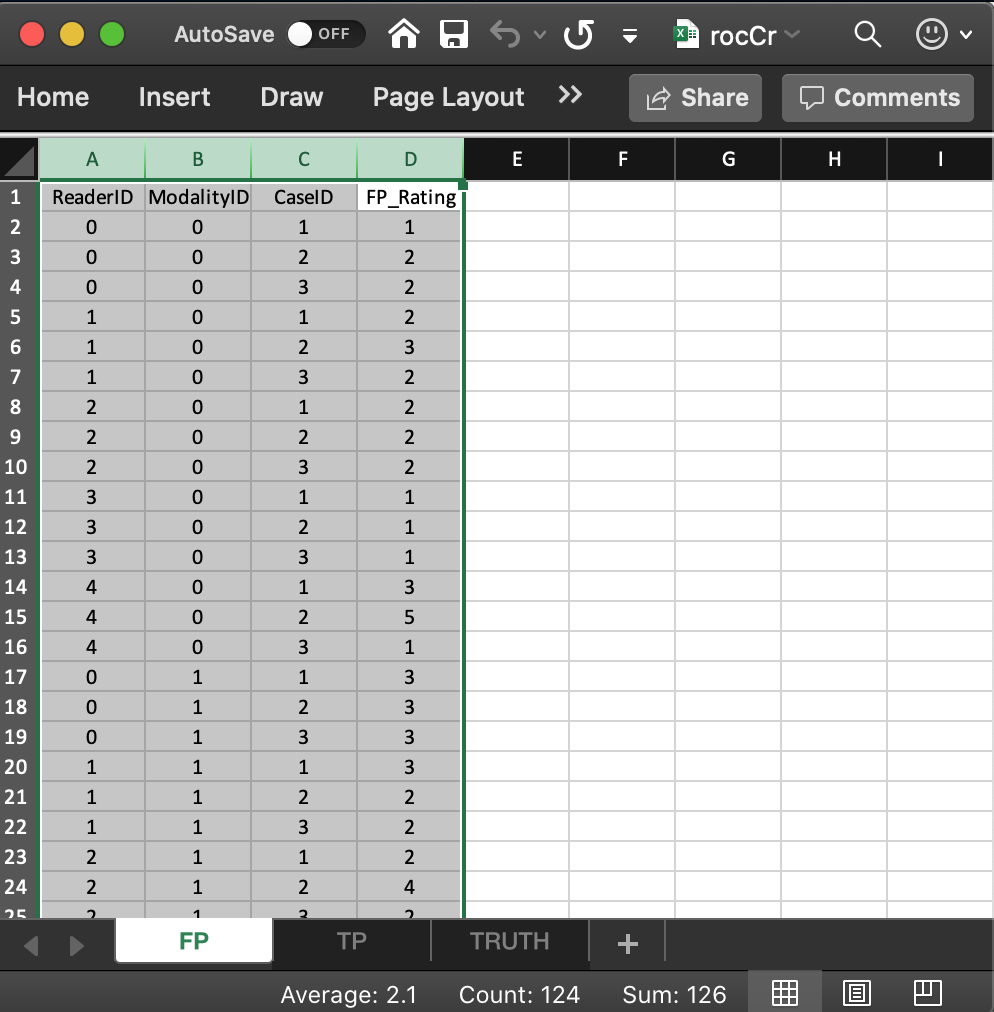
\includegraphics[width=1\textwidth,height=\textheight]{images/quick-start/rocCrFp.png}

\begin{itemize}
\tightlist
\item
  It consists of 4 columns, each of length 30 (\# of modalities X number of readers X number of non-diseased cases).
\item
  \texttt{ReaderID}: the reader labels: \texttt{0}, \texttt{1}, \texttt{2}, \texttt{3} and \texttt{4}. Each reader label occurs 6 times (\# of modalities X number of non-diseased cases).
\item
  \texttt{ModalityID}: the modality or treatment labels: \texttt{0} and \texttt{1}. Each label occurs 15 times (\# of readers X number of non-diseased cases).
\item
  \texttt{CaseID}: the case labels for non-diseased cases: \texttt{1}, \texttt{2} and \texttt{3}. Each label occurs 10 times (\# of modalities X \# of readers).
\item
  The label of a diseased case cannot occur in the FP worksheet. If it does the software generates an error.
\item
  \texttt{FP\_Rating}: the floating point ratings of non-diseased cases. Each row of this worksheet contains a rating corresponding to the values of \texttt{ReaderID}, \texttt{ModalityID} and \texttt{CaseID} for that row.
\end{itemize}

\hypertarget{quick-start-data-format-tp-worksheet}{%
\section{The true positive (TP) ratings}\label{quick-start-data-format-tp-worksheet}}

These are found in the \texttt{TP} or \texttt{LL} worksheet, see below.

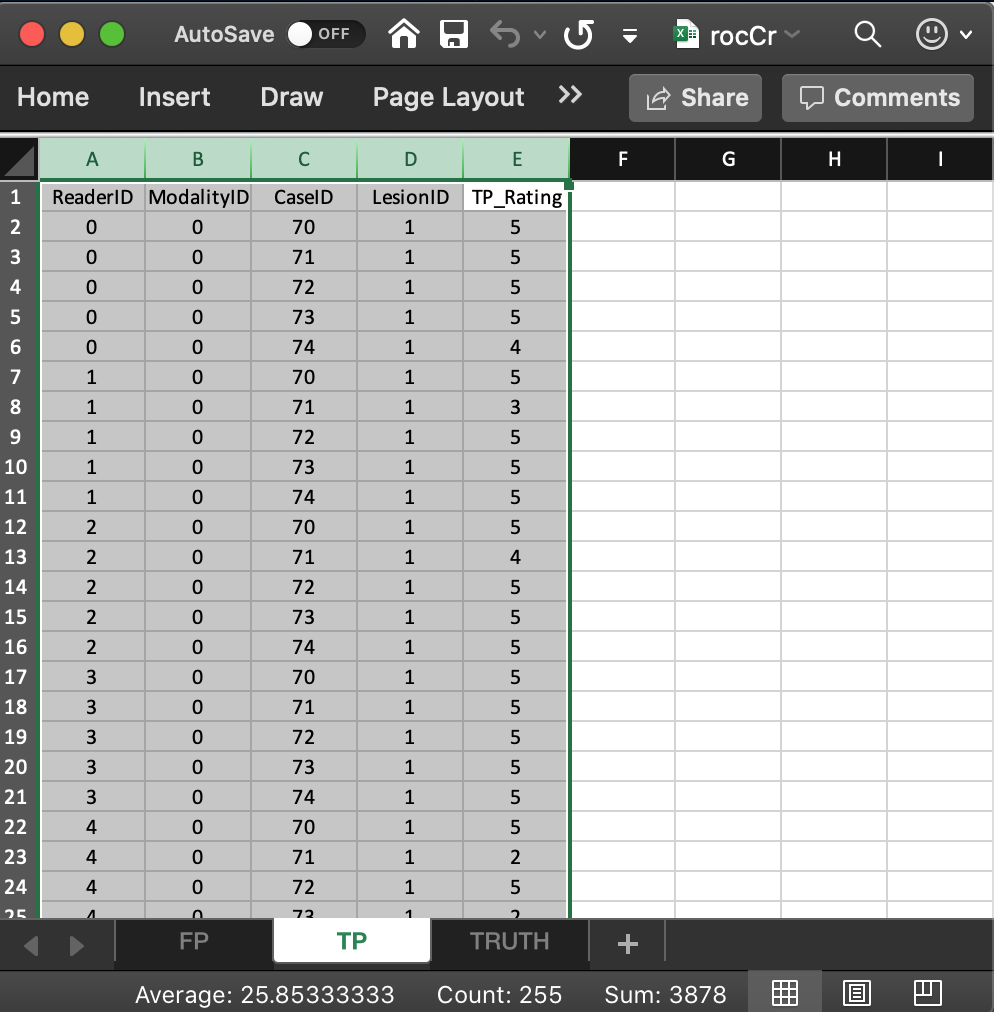
\includegraphics[width=1\textwidth,height=\textheight]{images/quick-start/rocCrTp.png}

\begin{itemize}
\tightlist
\item
  It consists of 5 columns, each of length 50 (\# of modalities X number of readers X number of diseased cases).
\item
  \texttt{ReaderID}: the reader labels: \texttt{0}, \texttt{1}, \texttt{2}, \texttt{3} and \texttt{4}. Each reader label occurs 10 times (\# of modalities X number of diseased cases).
\item
  \texttt{ModalityID}: the modality or treatment labels: \texttt{0} and \texttt{1}. Each label occurs 25 times (\# of readers X number of diseased cases).
\item
  \texttt{LesionID}: For an ROC dataset this column contains fifty 1's (each diseased case has one lesion).
\item
  \texttt{CaseID}: the case labels for non-diseased cases: \texttt{70}, \texttt{71}, \texttt{72}, \texttt{73} and \texttt{74}. Each label occurs 10 times (\# of modalities X \# of readers). For an ROC dataset the label of a non-diseased case cannot occur in the TP worksheet. If it does the software generates an error.
\item
  \texttt{TP\_Rating}: the floating point ratings of diseased cases. Each row of this worksheet contains a rating corresponding to the values of \texttt{ReaderID}, \texttt{ModalityID}, \texttt{LesionID} and \texttt{CaseID} for that row.
\end{itemize}

\hypertarget{quick-start-data-format-single-reader}{%
\section{A single reader dataset}\label{quick-start-data-format-single-reader}}

\begin{Shaded}
\begin{Highlighting}[]
\NormalTok{rocCr1R <-}\StringTok{ "R/quick-start/rocCr1R.xlsx"}
\NormalTok{x <-}\StringTok{ }\KeywordTok{DfReadDataFile}\NormalTok{(rocCr1R, }\DataTypeTok{newExcelFileFormat =} \OtherTok{TRUE}\NormalTok{)}
\KeywordTok{str}\NormalTok{(x)}
\CommentTok{#> List of 3}
\CommentTok{#>  $ ratings     :List of 3}
\CommentTok{#>   ..$ NL   : num [1:2, 1, 1:8, 1] 2 3 3 2 2 ...}
\CommentTok{#>   ..$ LL   : num [1:2, 1, 1:5, 1] 5 5 3 3 5 5 5 5 5 5}
\CommentTok{#>   ..$ LL_IL: logi NA}
\CommentTok{#>  $ lesions     :List of 3}
\CommentTok{#>   ..$ perCase: int [1:5] 1 1 1 1 1}
\CommentTok{#>   ..$ IDs    : num [1:5, 1] 1 1 1 1 1}
\CommentTok{#>   ..$ weights: num [1:5, 1] 1 1 1 1 1}
\CommentTok{#>  $ descriptions:List of 7}
\CommentTok{#>   ..$ fileName     : chr "rocCr1R"}
\CommentTok{#>   ..$ type         : chr "ROC"}
\CommentTok{#>   ..$ name         : logi NA}
\CommentTok{#>   ..$ truthTableStr: num [1:2, 1, 1:8, 1:2] 1 1 1 1 1 1 NA NA NA NA ...}
\CommentTok{#>   ..$ design       : chr "FCTRL"}
\CommentTok{#>   ..$ modalityID   : Named chr [1:2] "0" "1"}
\CommentTok{#>   .. ..- attr(*, "names")= chr [1:2] "0" "1"}
\CommentTok{#>   ..$ readerID     : Named chr "1"}
\CommentTok{#>   .. ..- attr(*, "names")= chr "1"}
\end{Highlighting}
\end{Shaded}

\hypertarget{quick-start-data-format-references}{%
\section{References}\label{quick-start-data-format-references}}

\hypertarget{quick-start-read-datafile}{%
\chapter{Reading the Excel data file}\label{quick-start-read-datafile}}

\hypertarget{quick-start-read-datafile-how-much-finished}{%
\section{TBA How much finished}\label{quick-start-read-datafile-how-much-finished}}

90\%

\hypertarget{quick-start-read-datafile-intro}{%
\section{Introduction}\label{quick-start-read-datafile-intro}}

In the previous chapter I described the format of the Excel file \texttt{R/quick-start/rocCr.xlsx} corresponding to a small factorial ROC dataset. Described here is how to read this file in order to create an \texttt{RJafroc} dataset. It introduces the \texttt{RJafroc} function \texttt{DfReadDataFile()}. Also shown are the correspondences between values in the Excel file and the dataset object.

\hypertarget{quick-start-read-datafile-structure-roc-dataset}{%
\section{The structure of an ROC dataset}\label{quick-start-read-datafile-structure-roc-dataset}}

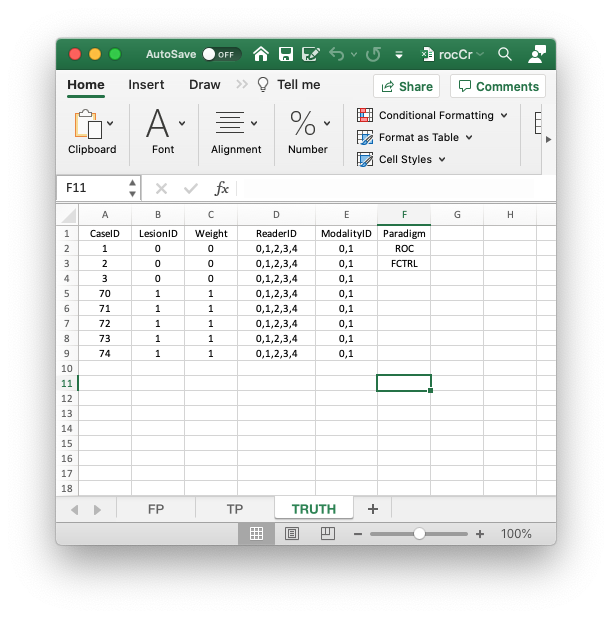
\includegraphics[width=1\textwidth,height=\textheight]{images/quick-start/rocCrTruth.png}

In the following code chunk the second statement reads the Excel file using the function \texttt{DfReadDataFile()} and saves it to object \texttt{x}. The third statement shows the structure of \texttt{x}.

\begin{Shaded}
\begin{Highlighting}[]
\NormalTok{rocCr <-}\StringTok{ "R/quick-start/rocCr.xlsx"}
\NormalTok{x <-}\StringTok{ }\KeywordTok{DfReadDataFile}\NormalTok{(rocCr, }\DataTypeTok{newExcelFileFormat =} \OtherTok{TRUE}\NormalTok{)}
\KeywordTok{str}\NormalTok{(x)}
\CommentTok{#> List of 3}
\CommentTok{#>  $ ratings     :List of 3}
\CommentTok{#>   ..$ NL   : num [1:2, 1:5, 1:8, 1] 1 3 2 3 2 2 1 2 3 2 ...}
\CommentTok{#>   ..$ LL   : num [1:2, 1:5, 1:5, 1] 5 5 5 5 5 5 5 5 5 5 ...}
\CommentTok{#>   ..$ LL_IL: logi NA}
\CommentTok{#>  $ lesions     :List of 3}
\CommentTok{#>   ..$ perCase: int [1:5] 1 1 1 1 1}
\CommentTok{#>   ..$ IDs    : num [1:5, 1] 1 1 1 1 1}
\CommentTok{#>   ..$ weights: num [1:5, 1] 1 1 1 1 1}
\CommentTok{#>  $ descriptions:List of 7}
\CommentTok{#>   ..$ fileName     : chr "rocCr"}
\CommentTok{#>   ..$ type         : chr "ROC"}
\CommentTok{#>   ..$ name         : logi NA}
\CommentTok{#>   ..$ truthTableStr: num [1:2, 1:5, 1:8, 1:2] 1 1 1 1 1 1 1 1 1 1 ...}
\CommentTok{#>   ..$ design       : chr "FCTRL"}
\CommentTok{#>   ..$ modalityID   : Named chr [1:2] "0" "1"}
\CommentTok{#>   .. ..- attr(*, "names")= chr [1:2] "0" "1"}
\CommentTok{#>   ..$ readerID     : Named chr [1:5] "0" "1" "2" "3" ...}
\CommentTok{#>   .. ..- attr(*, "names")= chr [1:5] "0" "1" "2" "3" ...}
\end{Highlighting}
\end{Shaded}

\begin{itemize}
\tightlist
\item
  In the above code chunk flag \texttt{newExcelFileFormat} is set to \texttt{TRUE} as otherwise columns D - F in the \texttt{Truth} worksheet are ignored and the dataset is assumed to be factorial, with \texttt{dataType} ``automatically'' determined from the contents of the FP and TP worksheets. \footnote{The assumptions underlying the ``automatic'' determination could be defeated by data entry errors.}
\item
  Flag \texttt{newExcelFileFormat\ =\ FALSE}, the default, is for compatibility with older JAFROC format Excel files, which did not have columns D - F in the \texttt{Truth} worksheet. Its usage is deprecated.
\item
  The dataset object \texttt{x} is a \texttt{list} variable with 3 members: \texttt{ratings}, \texttt{lesions} and \texttt{descriptions}.
\item
  The \texttt{x\$ratings} member contains 3 sub-lists.

  \begin{itemize}
  \tightlist
  \item
    The \texttt{x\$ratings\$NL} member, with dimension {[}2, 5, 8, 1{]}, contains the ratings of normal cases. The first dimension (2) is the number of treatments, the second (5) is the number of readers and the third (8) is the total number of cases. For ROC datasets the fourth dimension is always unity. The five extra values \footnote{with only 3 non-diseased cases why does one need 8 values?} in the third dimension, which are filled with \texttt{NAs}, are needed for compatibility with FROC datasets.
  \item
    The \texttt{x\$ratings\$LL}, with dimension {[}2, 5, 5, 1{]}, contains the ratings of abnormal cases. The third dimension (5) corresponds to the 5 diseased cases.
  \item
    The \texttt{x\$ratings\$LL\_IL} member, equal to NA'; this member is there for compatibility with LROC data, \texttt{\_IL} denotes incorrect-localizations.
  \end{itemize}
\item
  The \texttt{x\$lesions} member contains 3 sub-lists.

  \begin{itemize}
  \tightlist
  \item
    The \texttt{x\$lesions\$perCase} member is a vector with 5 ones representing the 5 diseased cases in the dataset.
  \item
    The \texttt{x\$lesions\$IDs} member is an array with 5 ones.
  \item
    The \texttt{x\$lesions\$weights} member is an array with 5 ones.
  \item
    These are irrelevant for ROC datasets. They are there for compatibility with FROC datasets.
  \end{itemize}
\item
  The \texttt{x\$descriptions} member contains 7 sub-lists.

  \begin{itemize}
  \tightlist
  \item
    The \texttt{x\$descriptions\$fileName} member is the base name of the file that was read to create this dataset, ``rocCr'' in the current example, otherwise it is \texttt{NA} (the latter would apply, for example, for a simulated dataset).
  \item
    The \texttt{x\$descriptions\$type} member indicates that this is an \texttt{ROC} dataset.
  \item
    The \texttt{x\$descriptions\$name} member is the name of this dataset, if it is an embedded dataset, otherwise \texttt{NA}.
  \item
    The \texttt{x\$descriptions\$truthTableStr} member, with dimension {[}2, 5, 8, 2{]}, quantifies the structure of the dataset, as explained in TBA Vignette \#3 (it is used to check for data entry errors).
  \item
    The \texttt{x\$descriptions\$design} member specifies the dataset design, which is ``FCTRL'' in the present example (a factorial dataset).
  \item
    The \texttt{x\$descriptions\$modalityID} member is a vector with two elements \texttt{"0"} and \texttt{"1"}, naming the two modalities.
  \item
    The \texttt{x\$readerID} member is a vector with five elements \texttt{"0"}, \texttt{"1"}, \texttt{"2"}, \texttt{"3"} and \texttt{"4"}, naming the five readers.
  \end{itemize}
\end{itemize}

\hypertarget{quick-start-read-datafile-correspondence-nl-fp}{%
\section{\texorpdfstring{Correspondence between \texttt{NL} member of dataset and the \texttt{FP} worksheet}{Correspondence between NL member of dataset and the FP worksheet}}\label{quick-start-read-datafile-correspondence-nl-fp}}

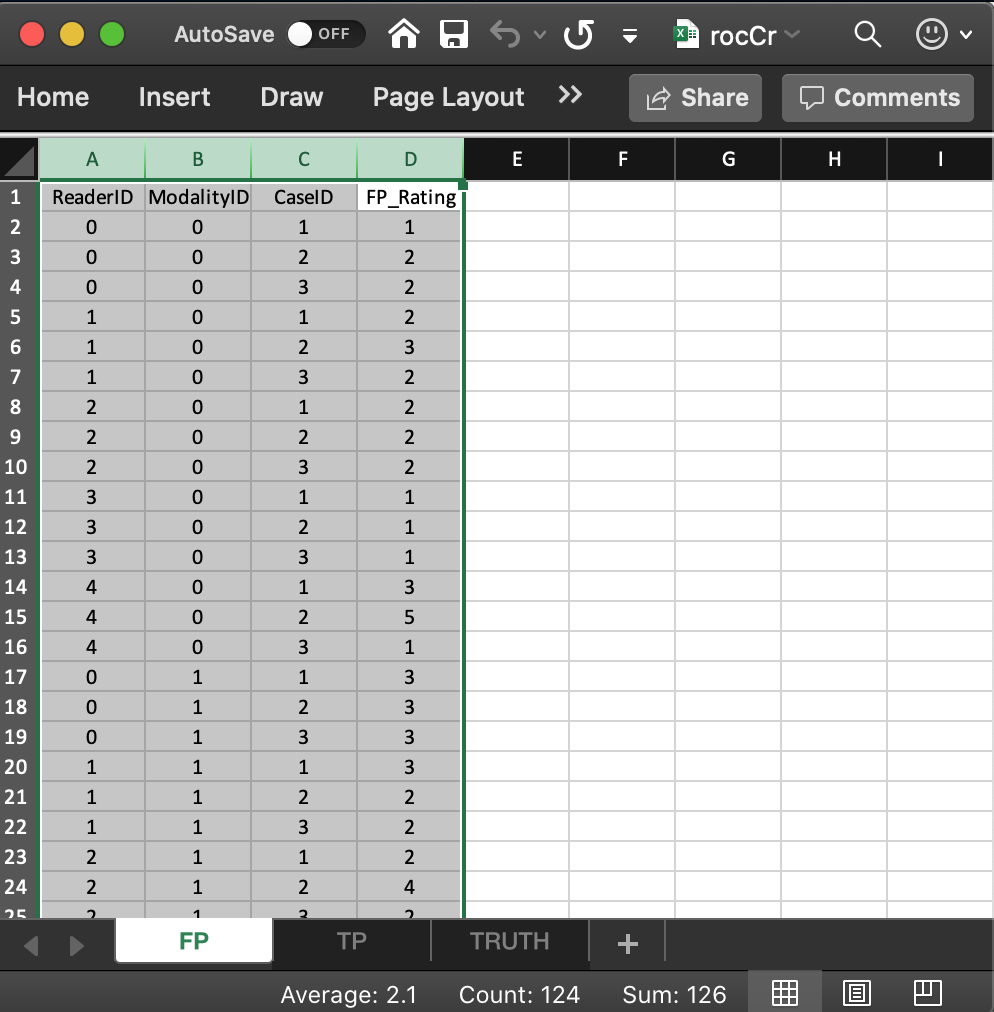
\includegraphics[width=1\textwidth,height=\textheight]{images/quick-start/rocCrFp.png}

\begin{itemize}
\tightlist
\item
  The list member \texttt{x\$ratings\$NL} is an array with \texttt{dim\ =\ c(2,5,8,1)}.

  \begin{itemize}
  \tightlist
  \item
    The first dimension (2) comes from the number of modalities.
  \item
    The second dimension (5) comes from the number of readers.
  \item
    The third dimension (8) comes from the \textbf{total} number of cases.
  \item
    The fourth dimension is alway 1 for an ROC dataset.
  \end{itemize}
\item
  The value of \texttt{x\$ratings\$NL{[}1,5,2,1{]}}, i.e., 5, corresponds to row 15 of the FP table, i.e., to \texttt{ModalityID} = 0, \texttt{ReaderID} = 4 and \texttt{CaseID} = 2.
\item
  The value of \texttt{x\$ratings\$NL{[}2,3,2,1{]}}, i.e., 4, corresponds to row 24 of the FP table, i.e., to \texttt{ModalityID} 1, \texttt{ReaderID} 2 and \texttt{CaseID} 2.
\item
  All values for case index \textgreater{} 3 and case index \textless= 8 are \texttt{-Inf}. For example the value of \texttt{x\$ratings\$NL{[}2,3,4,1{]}} is \texttt{-Inf}. This is because there are only 3 non-diseased cases. The extra length is needed for compatibility with FROC datasets.
\end{itemize}

\hypertarget{quick-start-read-datafile-correspondence-case-index-vs-case-id}{%
\section{Case-index vs.~caseID}\label{quick-start-read-datafile-correspondence-case-index-vs-case-id}}

\begin{itemize}
\tightlist
\item
  Regardless of what order they occur in the worksheet, the non-diseased cases are always indexed first. In the current example the case indices are 1, 2 and 3, corresponding to the three non-diseased cases with \texttt{caseIDs} equal to 1, 2 and 3.
\item
  Regardless of what order they occur in the worksheet, in the NL array the diseased cases are always indexed after the last non-diseased case. In the current example the case indices in the \texttt{NL} array are 4, 5, 6, 7 and 8, corresponding to the five diseased cases with \texttt{caseIDs} equal to 70, 71, 72, 73, and 74. In the \texttt{LL} array they are numbered 1, 2, 3, 4 and 5, corresponding to the five diseased cases with \texttt{caseIDs} equal to 70, 71, 72, 73, and 74. Some examples follow:
\item
  \texttt{x\$ratings\$NL{[}1,3,2,1{]}}, a FP rating, refers to \texttt{ModalityID} 0, \texttt{ReaderID} 2 and \texttt{CaseID} 2 (since the modality and reader IDs start with 0).
\item
  \texttt{x\$ratings\$NL{[}2,5,4,1{]}}, a FP rating, refers to \texttt{ModalityID} 1, \texttt{ReaderID} 4 and \texttt{CaseID} 70, the first diseased case; this is \texttt{-Inf}.
\item
  \texttt{x\$ratings\$NL{[}1,4,8,1{]}}, a FP rating, refers to \texttt{ModalityID} 0, \texttt{ReaderID} 3 and \texttt{CaseID} 74, the last diseased case; this is \texttt{-Inf}.
\item
  \texttt{x\$ratings\$NL{[}1,3,9,1{]}}, a FP rating, is an illegal value, as the third index cannot exceed 8.
\item
  \texttt{x\$ratings\$NL{[}1,3,8,2{]}}, a FP rating, is an illegal value, as the fourth index cannot exceed 1 for an ROC dataset.
\item
  \texttt{x\$ratings\$LL{[}1,3,1,1{]}}, a TP rating, refers to \texttt{ModalityID} 0, \texttt{ReaderID} 2 and \texttt{CaseID} 70, the first diseased case.
\item
  \texttt{x\$ratings\$LL{[}2,5,4,1{]}}, a TP rating, refers to \texttt{ModalityID} 1, \texttt{ReaderID} 4 and \texttt{CaseID} 73, the fourth diseased case.
\end{itemize}

\hypertarget{quick-start-read-datafile-correspondence-ll-tp}{%
\section{\texorpdfstring{Correspondence between \texttt{LL} member of dataset and the \texttt{TP} worksheet}{Correspondence between LL member of dataset and the TP worksheet}}\label{quick-start-read-datafile-correspondence-ll-tp}}

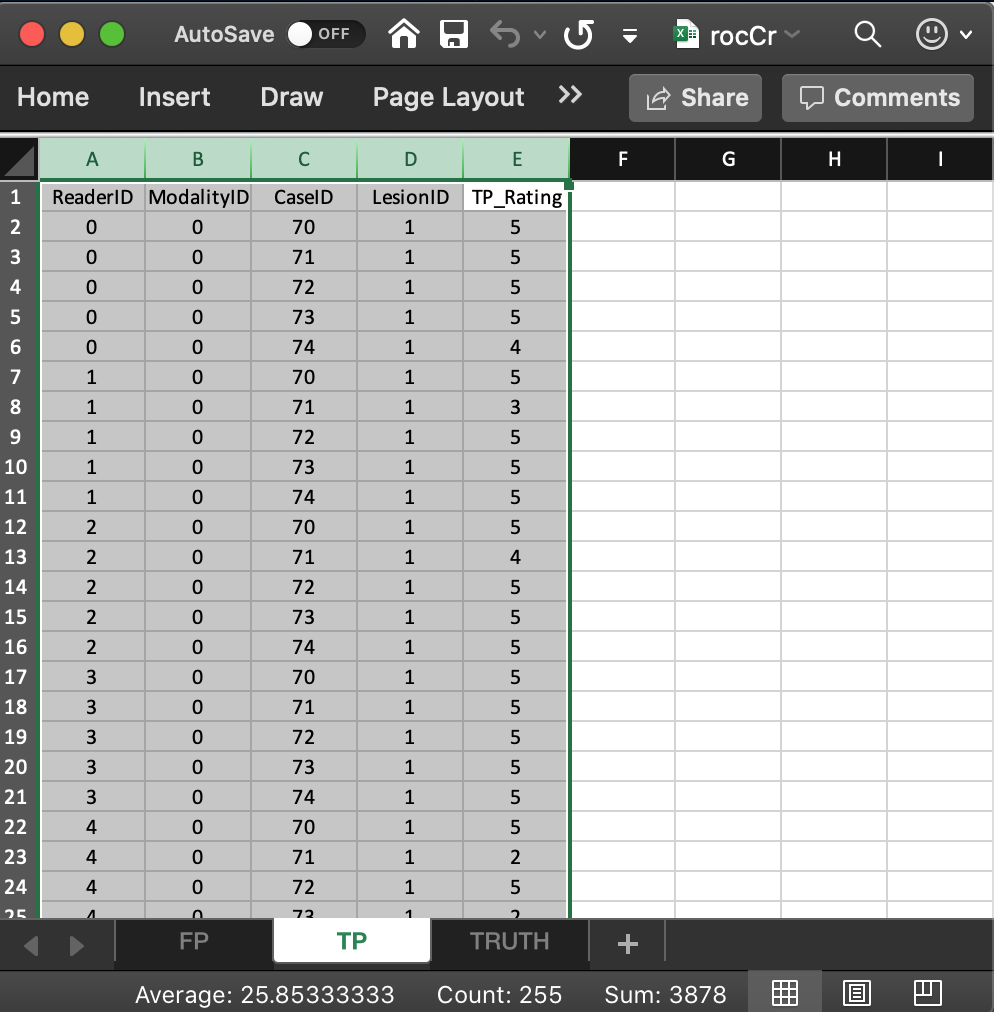
\includegraphics[width=1\textwidth,height=\textheight]{images/quick-start/rocCrTp.png}

\begin{itemize}
\tightlist
\item
  The list member \texttt{x\$ratings\$LL} is an array with \texttt{dim\ =\ c(2,5,5,1)}.

  \begin{itemize}
  \tightlist
  \item
    The first dimension (2) comes from the number of modalities.
  \item
    The second dimension (5) comes from the number of readers.
  \item
    The third dimension (5) comes from the number of diseased cases.
  \item
    The fourth dimension is always 1 for an ROC dataset.
  \end{itemize}
\item
  The value of \texttt{x\$ratings\$LL{[}1,1,5,1{]}}, i.e., 4, corresponds to row 6 of the TP table, i.e., to \texttt{ModalityID} = 0, \texttt{ReaderID} = 0 and \texttt{CaseID} = 74.
\item
  The value of \texttt{x\$ratings\$LL{[}1,2,2,1{]}}, i.e., 3, corresponds to row 8 of the TP table, i.e., to \texttt{ModalityID} = 0, \texttt{ReaderID} = 1 and \texttt{CaseID} = 71.
\item
  The value of \texttt{x\$ratings\$LL{[}1,4,4,1{]}}, i.e., 5, corresponds to row 21 of the TP table, i.e., to \texttt{ModalityID} = 0, \texttt{ReaderID} = 3 and \texttt{CaseID} = 74.
\item
  The value of \texttt{x\$ratings\$LL{[}1,5,2,1{]}}, i.e., 2, corresponds to row 23 of the TP table, i.e., to \texttt{ModalityID} = 0, \texttt{ReaderID} = 4 and \texttt{CaseID} = 71.
\item
  There are no \texttt{-Inf} values in \texttt{x\$ratings\$LL}: \texttt{any(x\$ratings\$LL\ ==\ -Inf)} = FALSE. This is true for any ROC dataset.
\end{itemize}

\hypertarget{quick-start-read-datafile-references}{%
\section{References}\label{quick-start-read-datafile-references}}

\hypertarget{quick-start-froc-data-format}{%
\chapter{Data format and reading FROC data}\label{quick-start-froc-data-format}}

\hypertarget{quick-start-froc-data-format-how-much-finished}{%
\section{TBA How much finished}\label{quick-start-froc-data-format-how-much-finished}}

90\%

\hypertarget{quick-start-froc-data-intro}{%
\section{Introduction}\label{quick-start-froc-data-intro}}

In the Free-response Receiver Operating Characteristic (FROC) paradigm the observer searches each case for signs of \textbf{localized disease} and marks and rates localized regions that are sufficiently suspicious for presence of disease. FROC data consists of \textbf{mark-rating pairs}, where each mark is a localized-region that was considered sufficiently suspicious for presence of a localized lesion and the rating is it's confidence level. As in the ROC paradigm, the rating can be an integer or quasi-continuous (e.g., 0 -- 100), or a floating point value, \emph{as long as higher numbers represent greater confidence in presence of a lesion at the indicated region}. This is termed a positive-directed confidence level scheme. By adopting a proximity criterion, the investigator classifies each mark as a lesion localization (\texttt{LL}) - if it is close to a real lesion - or a non-lesion localization (\texttt{NL}) otherwise.

The purpose of this chapter is to:

\begin{itemize}
\tightlist
\item
  Explain the data format of the input Excel file for FROC datasets.
\item
  Explain the format of the FROC dataset.
\item
  Explain the lesion distribution array returned by \texttt{UtilLesionDistrVector()}.
\item
  Explain the lesion weights array returned by \texttt{UtilLesionWeightsMatrix()}.
\item
  Details on the FROC paradigm are in my book \citep{chakraborty2017observer}.
\end{itemize}

The chapter is illustrated with a toy data file, \texttt{R/quick-start/frocCr.xlsx} in which readers `0', `1' and `2' interpret 8 cases in two modalities, `0' and `1'. The design is `factorial', abbreviated to \texttt{FCTRL} in the software; this is also termed a `fully-crossed' design. The Excel file has three worksheets named \texttt{Truth}, \texttt{NL} (or \texttt{FP}) and \texttt{LL} (or \texttt{TP}).

\hypertarget{quick-start-froc-data-truth}{%
\section{\texorpdfstring{The \texttt{Truth} worksheet}{The Truth worksheet}}\label{quick-start-froc-data-truth}}

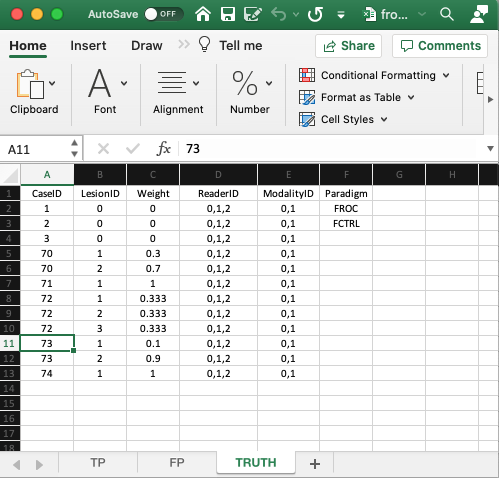
\includegraphics[width=1\textwidth,height=\textheight]{images/quick-start/frocCrTruth.png}

\begin{itemize}
\tightlist
\item
  The \texttt{Truth} worksheet contains 6 columns: \texttt{CaseID}, \texttt{LesionID}, \texttt{Weight}, \texttt{ReaderID}, \texttt{ModalityID} and \texttt{Paradigm}.
\item
  Since a diseased case may have more than one lesion, the first five columns contain \textbf{at least} as many rows as there are cases (images) in the dataset. There are 8 cases in the dataset and 12 rows of data, because some of the diseased cases contain more than one lesion.
\item
  \texttt{CaseID}: unique \textbf{integers} representing the cases in the dataset: `1', `2', `3', the 3 non-diseased cases, and `70', `71', `72', `73', `74', the 5 diseased cases. The ordering of the numbers is inconsequential. \footnote{\texttt{CaseID} should not be so large that it cannot be represented in Excel by an integer; to be safe use unsigned short 8-bit integers. For example, 108057200 or 9971103254 are too large to be a valid \texttt{caseID} and may cause errors.}
\item
  \texttt{LesionID}: integers 0, 1, 2, etc.,

  \begin{itemize}
  \tightlist
  \item
    Each 0 represents a non-diseased case,
  \item
    Each 1 represents the \emph{first} lesion on a diseased case, 2 the \emph{second} lesion, if present, and so on.
  \item
    This field is zero for non-diseased cases `1', `2', `3'.
  \item
    For the first diseased case, i.e., `70', it is 1 for the first lesion and 2 for the second lesion.
  \item
    For the second diseased case i.e., `71', it is 1, as this case has only one lesion.
  \item
    For the third diseased case, i.e., `72', it is 1 for the first lesion, 2 for the second lesion and 3 for the third lesion.
  \item
    For the fourth diseased case, i.e., `73', it is 1 for the first lesion and 2 for the second lesion.
  \item
    For the fifth diseased case i.e., `74', it is 1, as this case has only one lesion.
  \end{itemize}
\item
  There are 3 non-diseased cases in the dataset (the number of 0's in the \texttt{LesionID} column).
\item
  There are 5 diseased cases in the dataset (the number of 1's in the \texttt{LesionID} column).
\item
  \texttt{Weight} or clinical importance - e.g., mortality associated with lesion:

  \begin{itemize}
  \tightlist
  \item
    non-negative floating point values
  \item
    0 for each non-diseased case
  \item
    For each diseased case values that sum to unity.
  \item
    A simple way to assign equal weights to all lesions in a case is to fill the \texttt{Weight} column with zeroes.
  \end{itemize}
\item
  \texttt{LesionID}

  \begin{itemize}
  \tightlist
  \item
    Diseased case \texttt{70} has two lesions, with \texttt{LesionID}s `1' and `2', and weights 0.3 and 0.7.
  \item
    Diseased case \texttt{71} has one lesion, with \texttt{LesionID} = 1, and \texttt{Weight} = 1.
  \item
    Diseased case \texttt{72} has three lesions, with \texttt{LesionID}s 1, 2 and 3 and weights 1/3 each.
  \item
    Diseased case \texttt{73} has two lesions, with \texttt{LesionID}s 1, and 2 and weights 0.1 and 0.9.
  \item
    Diseased case \texttt{74} has one lesion, with \texttt{LesionID} = 1 and \texttt{Weight} = 1.
  \end{itemize}
\item
  \texttt{ReaderID}: a comma-separated listing of readers, each represented by a unique \textbf{text label}, that have interpreted the case. In the example shown below each cell has the value `0, 1, 2'.
\item
  There are 3 readers in the dataset, as each cell in the \texttt{ReaderID} column contains `0, 1, 2'.
\item
  \texttt{ModalityID}: a comma-separated listing of modalities (or treatments), each represented by a unique \textbf{integer}, that apply to each case. In the example each cell has the value \texttt{0,\ 1}. \textbf{Each cell has to be text formatted.}
\item
  There are 2 modalities in the dataset, as each cell in the \texttt{ModalityID} column contains `0, 1'.
\item
  \texttt{Paradigm}: The contents are \texttt{FROC} and \texttt{FCTRL}: this is an \texttt{FROC} dataset and the design is ``factorial''.
\end{itemize}

\hypertarget{quick-start-froc-data-structure}{%
\section{Reading the FROC dataset}\label{quick-start-froc-data-structure}}

The example shown above corresponds to file \texttt{R/quick-start/frocCr.xlsx} in the project directory. The next code chunk reads this file into an \texttt{R} object \texttt{x}.

\begin{Shaded}
\begin{Highlighting}[]
\NormalTok{frocCr <-}\StringTok{ "R/quick-start/frocCr.xlsx"}
\NormalTok{x <-}\StringTok{ }\KeywordTok{DfReadDataFile}\NormalTok{(frocCr, }\DataTypeTok{newExcelFileFormat =} \OtherTok{TRUE}\NormalTok{)}
\KeywordTok{str}\NormalTok{(x)}
\CommentTok{#> List of 3}
\CommentTok{#>  $ ratings     :List of 3}
\CommentTok{#>   ..$ NL   : num [1:2, 1:3, 1:8, 1:2] 1.02 2.89 2.21 3.01 2.14 ...}
\CommentTok{#>   ..$ LL   : num [1:2, 1:3, 1:5, 1:3] 5.28 5.2 5.14 4.77 4.66 4.87 3.01 3.27 3.31 3.19 ...}
\CommentTok{#>   ..$ LL_IL: logi NA}
\CommentTok{#>  $ lesions     :List of 3}
\CommentTok{#>   ..$ perCase: int [1:5] 2 1 3 2 1}
\CommentTok{#>   ..$ IDs    : num [1:5, 1:3] 1 1 1 1 1 ...}
\CommentTok{#>   ..$ weights: num [1:5, 1:3] 0.3 1 0.333 0.1 1 ...}
\CommentTok{#>  $ descriptions:List of 7}
\CommentTok{#>   ..$ fileName     : chr "frocCr"}
\CommentTok{#>   ..$ type         : chr "FROC"}
\CommentTok{#>   ..$ name         : logi NA}
\CommentTok{#>   ..$ truthTableStr: num [1:2, 1:3, 1:8, 1:4] 1 1 1 1 1 1 1 1 1 1 ...}
\CommentTok{#>   ..$ design       : chr "FCTRL"}
\CommentTok{#>   ..$ modalityID   : Named chr [1:2] "0" "1"}
\CommentTok{#>   .. ..- attr(*, "names")= chr [1:2] "0" "1"}
\CommentTok{#>   ..$ readerID     : Named chr [1:3] "0" "1" "2"}
\CommentTok{#>   .. ..- attr(*, "names")= chr [1:3] "0" "1" "2"}
\end{Highlighting}
\end{Shaded}

This follows the general description in Chapter \ref{quick-start-data-format}. The differences are described below.

\begin{itemize}
\tightlist
\item
  The \texttt{x\$descriptions\$type} member indicates that this is an \texttt{FROC} dataset.
\item
  The \texttt{x\$lesions\$perCase} member is a vector whose contents reflect the number of lesions in each diseased case, i.e., 2, 1, 3, 2, 1 in the current example.
\item
  The \texttt{x\$lesions\$IDs} member indicates the labeling of the lesions in each diseased case.
\end{itemize}

\begin{Shaded}
\begin{Highlighting}[]
\NormalTok{x}\OperatorTok{$}\NormalTok{lesions}\OperatorTok{$}\NormalTok{IDs}
\CommentTok{#>      [,1] [,2] [,3]}
\CommentTok{#> [1,]    1    2 -Inf}
\CommentTok{#> [2,]    1 -Inf -Inf}
\CommentTok{#> [3,]    1    2    3}
\CommentTok{#> [4,]    1    2 -Inf}
\CommentTok{#> [5,]    1 -Inf -Inf}
\end{Highlighting}
\end{Shaded}

\begin{itemize}
\tightlist
\item
  This shows that the lesions on the first diseased case are labeled `1' and `2'. The \texttt{-Inf} is a filler used to denote a missing value. The second diseased case has one lesion labeled `1'. The third diseased case has three lesions labeled `1', `2' and `3', etc.
\item
  The \texttt{lesionWeight} member is the clinical importance of each lesion. Lacking specific clinical reasons, the lesions should be equally weighted; this is \emph{not} true for this toy dataset.
\end{itemize}

\begin{Shaded}
\begin{Highlighting}[]
\NormalTok{x}\OperatorTok{$}\NormalTok{lesions}\OperatorTok{$}\NormalTok{weights}
\CommentTok{#>           [,1]      [,2]      [,3]}
\CommentTok{#> [1,] 0.3000000 0.7000000      -Inf}
\CommentTok{#> [2,] 1.0000000      -Inf      -Inf}
\CommentTok{#> [3,] 0.3333333 0.3333333 0.3333333}
\CommentTok{#> [4,] 0.1000000 0.9000000      -Inf}
\CommentTok{#> [5,] 1.0000000      -Inf      -Inf}
\end{Highlighting}
\end{Shaded}

\begin{itemize}
\tightlist
\item
  The first diseased case has two lesions, the first has weight 0.3 and the second has weight 0.7.
\item
  The second diseased case has one lesion with weight 1.
\item
  The third diseased case has three equally weighted lesions, each with weight 1/3. Etc.
\end{itemize}

\hypertarget{quick-start-froc-data-fp}{%
\section{The false positive (FP) ratings}\label{quick-start-froc-data-fp}}

These are found in the \texttt{FP} or \texttt{NL} worksheet.

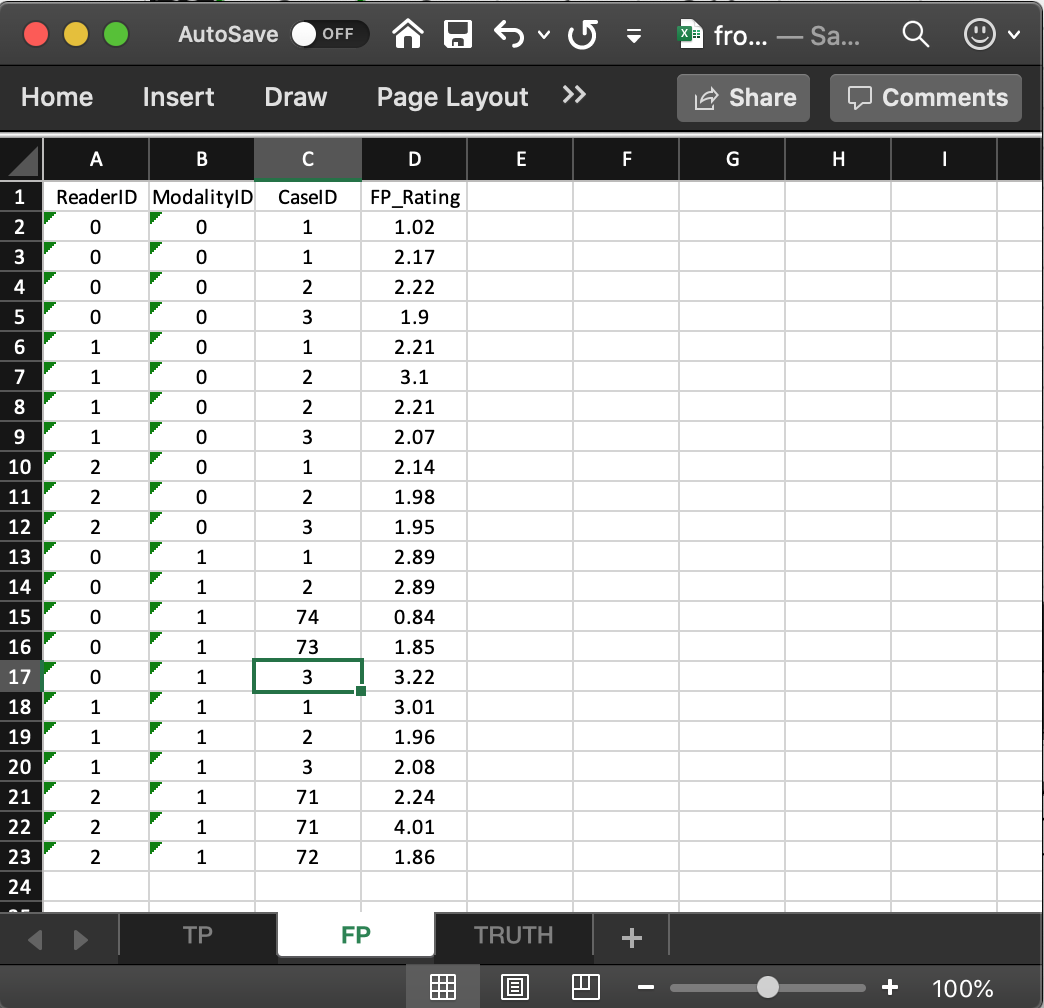
\includegraphics[width=1\textwidth,height=\textheight]{images/quick-start/frocCrNL.png}

\begin{itemize}
\tightlist
\item
  It consists of 4 columns, of equal length. The common length is an integer random variable greater than or equal to zero. It could be zero if the dataset has no NL marks (a possibility if the lesions are very easy to find and the observer has perfect performance).\\
\item
  In the example dataset, the common length is 22.
\item
  \texttt{ReaderID}: the reader labels: these must be \texttt{0}, \texttt{1}, or \texttt{2}, as declared in the \texttt{Truth} worksheet.
\item
  \texttt{ModalityID}: the modality labels: must be \texttt{0} or \texttt{1}, as declared in the \texttt{Truth} worksheet.
\item
  \texttt{CaseID}: the labels of cases with \texttt{NL} marks. In the FROC paradigm \texttt{NL} events can occur on non-diseased \textbf{and} diseased cases.
\item
  \texttt{FP\_Rating}: the floating point ratings of \texttt{NL} marks. Each row of this worksheet yields a rating corresponding to the values of \texttt{ReaderID}, \texttt{ModalityID} and \texttt{CaseID} for that row.
\item
  For \texttt{ModalityID} 0, \texttt{ReaderID} 0 and \texttt{CaseID} 1 (the first non-diseased case declared in the \texttt{Truth} worksheet), there is a single \texttt{NL} mark that was rated 1.02, corresponding to row 2 of the \texttt{FP} worksheet.
\item
  Diseased cases with \texttt{NL} marks are also recorded in the \texttt{FP} worksheet. Some examples are seen at rows 15, 16 and 21, 22, 23.
\item
  Rows 21 and 22 show that \texttt{caseID} = 71 got two \texttt{NL} marks, rated 2.24, 4.01.
\item
  Since this is the \emph{only} case with two NL marks, it determines the length of the fourth dimension of the \texttt{x\$ratings\$NL} list member, 2. Absent this case, the length would have been one.
\item
  The case with the most \texttt{NL} marks determines the length of the fourth dimension of the \texttt{x\$ratings\$NL} list member.
\item
  The reader should confirm that the ratings in \texttt{x\$ratings\$NL} reflect the contents of the \texttt{FP} worksheet.
\end{itemize}

\hypertarget{quick-start-froc-data-tp}{%
\section{The true positive (TP) ratings}\label{quick-start-froc-data-tp}}

These are found in the \texttt{TP} or \texttt{LL} worksheet, see below.

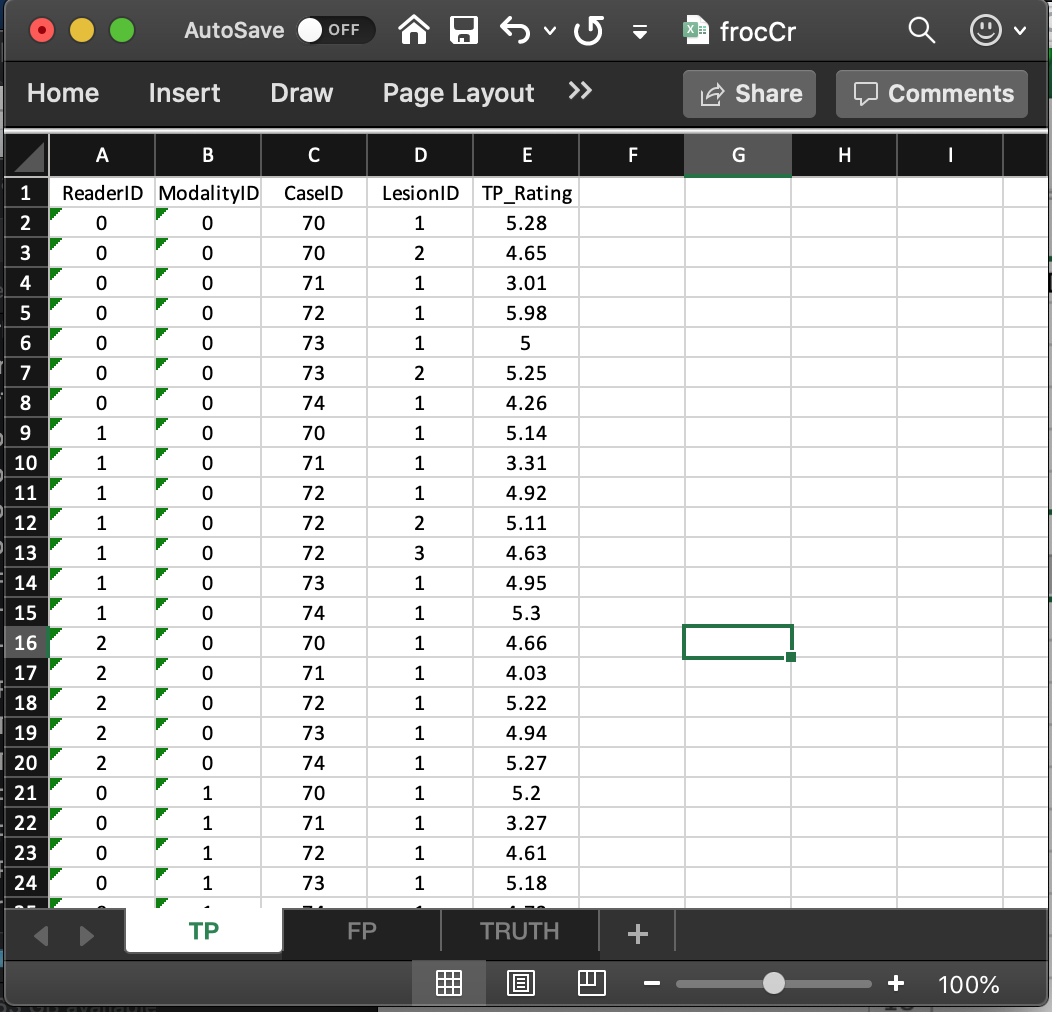
\includegraphics[width=1\textwidth,height=\textheight]{images/quick-start/frocCrLL.png}

\begin{itemize}
\tightlist
\item
  This worksheet can only have diseased cases. The presence of a non-diseased case in this worksheet will generate an error.
\item
  The common vertical length, 31 in this example, is a-priori unpredictable. The maximum possible length, assuming every lesion is marked for each modality, reader and diseased case, is 9 X 2 X 3 = 54. The 9 comes from the total number of non-zero entries in the \texttt{LesionID} column of the \texttt{Truth} worksheet, the 2 from the number of modalities and 3 from the number of readers.
\item
  The fact that the actual length (31) is smaller than the maximum length (54) means that there are combinations of modality, reader and diseased cases on which some lesions were not marked.
\item
  As examples, line 2 in the worksheet, the first lesion in \texttt{CaseID} equal to \texttt{70} was marked (and rated 5.28) in \texttt{ModalityID} \texttt{0} and \texttt{ReaderID} \texttt{0}. Line 3 in the worksheet, the second lesion in \texttt{CaseID} equal to \texttt{70} was also marked (and rated 4.65) in \texttt{ModalityID} \texttt{0} and \texttt{ReaderID} \texttt{0}. However, lesions 2 and 3 in \texttt{CaseID} = 72 were not marked (line 5 in the worksheet indicates that for this modality-reader-case combination only the first lesion was marked).
\item
  The length of the fourth dimension of the \texttt{x\$ratings\$LL} list member, 3 in the present example, is determined by the diseased case (72) with the most lesions in the \texttt{Truth} worksheet.
\item
  The reader should confirm that the ratings in \texttt{x\$ratings\$LL} reflect the contents of the \texttt{TP} worksheet.
\end{itemize}

\hypertarget{quick-start-froc-data-distribution-diseased-cases}{%
\section{On the distribution of numbers of lesions in diseased cases}\label{quick-start-froc-data-distribution-diseased-cases}}

\begin{itemize}
\tightlist
\item
  Consider a much larger dataset, \texttt{dataset11}, with structure as shown below (for descriptions of all embedded datasets the \texttt{RJafroc} documentation):
\end{itemize}

\begin{Shaded}
\begin{Highlighting}[]
\NormalTok{x <-}\StringTok{ }\NormalTok{dataset11}
\KeywordTok{str}\NormalTok{(x)}
\CommentTok{#> List of 3}
\CommentTok{#>  $ ratings     :List of 3}
\CommentTok{#>   ..$ NL   : num [1:4, 1:5, 1:158, 1:4] -Inf -Inf -Inf -Inf -Inf ...}
\CommentTok{#>   ..$ LL   : num [1:4, 1:5, 1:115, 1:20] -Inf -Inf -Inf -Inf -Inf ...}
\CommentTok{#>   ..$ LL_IL: logi NA}
\CommentTok{#>  $ lesions     :List of 3}
\CommentTok{#>   ..$ perCase: int [1:115] 6 4 7 1 3 3 3 8 11 2 ...}
\CommentTok{#>   ..$ IDs    : num [1:115, 1:20] 1 1 1 1 1 1 1 1 1 1 ...}
\CommentTok{#>   ..$ weights: num [1:115, 1:20] 0.167 0.25 0.143 1 0.333 ...}
\CommentTok{#>  $ descriptions:List of 7}
\CommentTok{#>   ..$ fileName     : chr "dataset11"}
\CommentTok{#>   ..$ type         : chr "FROC"}
\CommentTok{#>   ..$ name         : chr "DOBBINS-1"}
\CommentTok{#>   ..$ truthTableStr: num [1:4, 1:5, 1:158, 1:21] 1 1 1 1 1 1 1 1 1 1 ...}
\CommentTok{#>   ..$ design       : chr "FCTRL"}
\CommentTok{#>   ..$ modalityID   : Named chr [1:4] "1" "2" "3" "4"}
\CommentTok{#>   .. ..- attr(*, "names")= chr [1:4] "1" "2" "3" "4"}
\CommentTok{#>   ..$ readerID     : Named chr [1:5] "1" "2" "3" "4" ...}
\CommentTok{#>   .. ..- attr(*, "names")= chr [1:5] "1" "2" "3" "4" ...}
\end{Highlighting}
\end{Shaded}

\begin{itemize}
\tightlist
\item
  Focus for now in the 115 diseased cases.
\item
  The numbers of lesions in these cases is contained in \texttt{x\$lesions\$perCase}.
\end{itemize}

\begin{Shaded}
\begin{Highlighting}[]
\NormalTok{x}\OperatorTok{$}\NormalTok{lesions}\OperatorTok{$}\NormalTok{perCase}
\CommentTok{#>   [1]  6  4  7  1  3  3  3  8 11  2  4  6  2 16  5  2  8  3  4  7 11  1  4  3  4}
\CommentTok{#>  [26]  4  7  3  2  5  2  2  7  6  6  4 10 20 12  6  4  7 12  5  1  1  5  1  2  8}
\CommentTok{#>  [51]  3  1  2  2  3  2  8 16 10  1  2  2  6  3  2  2  4  6 10 11  1  2  6  2  4}
\CommentTok{#>  [76]  5  2  9  6  6  8  3  8  7  1  1  6  3  2  1  9  8  8  2  2 12  1  1  1  1}
\CommentTok{#> [101]  1  3  1  2  2  1  1  1  1  3  1  1  1  2  1}
\end{Highlighting}
\end{Shaded}

\begin{itemize}
\tightlist
\item
  For example, the first diseased case contains 6 lesions, the second contains 4 lesions, the third contains 7 lesions, etc. and the last diseased case contains 1 lesion.
\item
  To get an idea of the distribution of the numbers of lesions per diseased cases, one could interrogate this vector as shown below using the \texttt{which()} function:
\end{itemize}

\begin{Shaded}
\begin{Highlighting}[]
\ControlFlowTok{for}\NormalTok{ (el }\ControlFlowTok{in} \DecValTok{1}\OperatorTok{:}\KeywordTok{max}\NormalTok{(x}\OperatorTok{$}\NormalTok{lesions}\OperatorTok{$}\NormalTok{perCase)) }\KeywordTok{cat}\NormalTok{(}
  \StringTok{"number of diseased cases with"}\NormalTok{, el, }\StringTok{"lesions = "}\NormalTok{, }
  \KeywordTok{length}\NormalTok{(}\KeywordTok{which}\NormalTok{(x}\OperatorTok{$}\NormalTok{lesions}\OperatorTok{$}\NormalTok{perCase }\OperatorTok{==}\StringTok{ }\NormalTok{el)), }\StringTok{"}\CharTok{\textbackslash{}n}\StringTok{"}\NormalTok{)}
\CommentTok{#> number of diseased cases with 1 lesions =  25 }
\CommentTok{#> number of diseased cases with 2 lesions =  23 }
\CommentTok{#> number of diseased cases with 3 lesions =  13 }
\CommentTok{#> number of diseased cases with 4 lesions =  10 }
\CommentTok{#> number of diseased cases with 5 lesions =  5 }
\CommentTok{#> number of diseased cases with 6 lesions =  11 }
\CommentTok{#> number of diseased cases with 7 lesions =  6 }
\CommentTok{#> number of diseased cases with 8 lesions =  8 }
\CommentTok{#> number of diseased cases with 9 lesions =  2 }
\CommentTok{#> number of diseased cases with 10 lesions =  3 }
\CommentTok{#> number of diseased cases with 11 lesions =  3 }
\CommentTok{#> number of diseased cases with 12 lesions =  3 }
\CommentTok{#> number of diseased cases with 13 lesions =  0 }
\CommentTok{#> number of diseased cases with 14 lesions =  0 }
\CommentTok{#> number of diseased cases with 15 lesions =  0 }
\CommentTok{#> number of diseased cases with 16 lesions =  2 }
\CommentTok{#> number of diseased cases with 17 lesions =  0 }
\CommentTok{#> number of diseased cases with 18 lesions =  0 }
\CommentTok{#> number of diseased cases with 19 lesions =  0 }
\CommentTok{#> number of diseased cases with 20 lesions =  1}
\end{Highlighting}
\end{Shaded}

\begin{itemize}
\tightlist
\item
  This tells us that 25 cases contain 1 lesion
\item
  Likewise, 23 cases contain 2 lesions
\item
  Etc.
\end{itemize}

\hypertarget{quick-start-froc-data-lesion-distribution}{%
\subsection{\texorpdfstring{Definition of \texttt{lesDistr} array}{Definition of lesDistr array}}\label{quick-start-froc-data-lesion-distribution}}

\begin{itemize}
\tightlist
\item
  What is the fraction of (diseased) cases with 1 lesion, 2 lesions etc.
\end{itemize}

\begin{Shaded}
\begin{Highlighting}[]
\ControlFlowTok{for}\NormalTok{ (el }\ControlFlowTok{in} \DecValTok{1}\OperatorTok{:}\KeywordTok{max}\NormalTok{(x}\OperatorTok{$}\NormalTok{lesions}\OperatorTok{$}\NormalTok{perCase)) }\KeywordTok{cat}\NormalTok{(}\StringTok{"fraction of diseased cases with"}\NormalTok{, el, }\StringTok{"lesions = "}\NormalTok{, }
                                              \KeywordTok{length}\NormalTok{(}\KeywordTok{which}\NormalTok{(x}\OperatorTok{$}\NormalTok{lesions}\OperatorTok{$}\NormalTok{perCase }\OperatorTok{==}\StringTok{ }\NormalTok{el))}\OperatorTok{/}\KeywordTok{length}\NormalTok{(x}\OperatorTok{$}\NormalTok{ratings}\OperatorTok{$}\NormalTok{LL[}\DecValTok{1}\NormalTok{,}\DecValTok{1}\NormalTok{,,}\DecValTok{1}\NormalTok{]), }\StringTok{"}\CharTok{\textbackslash{}n}\StringTok{"}\NormalTok{)}
\CommentTok{#> fraction of diseased cases with 1 lesions =  0.2173913 }
\CommentTok{#> fraction of diseased cases with 2 lesions =  0.2 }
\CommentTok{#> fraction of diseased cases with 3 lesions =  0.1130435 }
\CommentTok{#> fraction of diseased cases with 4 lesions =  0.08695652 }
\CommentTok{#> fraction of diseased cases with 5 lesions =  0.04347826 }
\CommentTok{#> fraction of diseased cases with 6 lesions =  0.09565217 }
\CommentTok{#> fraction of diseased cases with 7 lesions =  0.05217391 }
\CommentTok{#> fraction of diseased cases with 8 lesions =  0.06956522 }
\CommentTok{#> fraction of diseased cases with 9 lesions =  0.0173913 }
\CommentTok{#> fraction of diseased cases with 10 lesions =  0.02608696 }
\CommentTok{#> fraction of diseased cases with 11 lesions =  0.02608696 }
\CommentTok{#> fraction of diseased cases with 12 lesions =  0.02608696 }
\CommentTok{#> fraction of diseased cases with 13 lesions =  0 }
\CommentTok{#> fraction of diseased cases with 14 lesions =  0 }
\CommentTok{#> fraction of diseased cases with 15 lesions =  0 }
\CommentTok{#> fraction of diseased cases with 16 lesions =  0.0173913 }
\CommentTok{#> fraction of diseased cases with 17 lesions =  0 }
\CommentTok{#> fraction of diseased cases with 18 lesions =  0 }
\CommentTok{#> fraction of diseased cases with 19 lesions =  0 }
\CommentTok{#> fraction of diseased cases with 20 lesions =  0.008695652}
\end{Highlighting}
\end{Shaded}

\begin{itemize}
\tightlist
\item
  This tells us that fraction 0.217 of (diseased) cases contain 1 lesion
\item
  And fraction 0.2 of (diseased) cases contain 2 lesions
\item
  Etc.
\item
  This information is obtained using the function \texttt{UtilLesionDistrVector()}
\end{itemize}

\begin{Shaded}
\begin{Highlighting}[]
\NormalTok{lesDistr <-}\StringTok{ }\KeywordTok{UtilLesionDistrVector}\NormalTok{(x)}
\NormalTok{lesDistr}
\CommentTok{#>  [1] 0.217391304 0.200000000 0.113043478 0.086956522 0.043478261 0.095652174}
\CommentTok{#>  [7] 0.052173913 0.069565217 0.017391304 0.026086957 0.026086957 0.026086957}
\CommentTok{#> [13] 0.017391304 0.008695652}
\end{Highlighting}
\end{Shaded}

\begin{itemize}
\tightlist
\item
  TBA The \texttt{UtilLesionDistrVector()} function returns an array with two columns and number of rows equal to the number of \emph{distinct non-zero} values of lesions per case.
\item
  The first column contains the number of distinct non-zero values of lesions per case, 14 in the current example.
\item
  The second column contains the fraction of diseased cases with the number of lesions indicated in the first column.
\item
  The second column must sum to unity
\end{itemize}

\begin{Shaded}
\begin{Highlighting}[]
\KeywordTok{sum}\NormalTok{(}\KeywordTok{UtilLesionDistrVector}\NormalTok{(x))}
\CommentTok{#> [1] 1}
\end{Highlighting}
\end{Shaded}

\begin{itemize}
\tightlist
\item
  The lesion distribution array will come in handy when it comes to predicting the operating characteristics from using the Radiological Search Model (RSM), as detailed in TBA Chapter 17.
\end{itemize}

\hypertarget{quick-start-froc-data-lesion-weights}{%
\section{\texorpdfstring{TBA Definition of \texttt{lesWghtDistr} array}{TBA Definition of lesWghtDistr array}}\label{quick-start-froc-data-lesion-weights}}

\begin{itemize}
\tightlist
\item
  This is returned by \texttt{UtilLesionWeightsDistr()}.
\item
  This contains the same number of rows as \texttt{lesDistr}.
\item
  The number of columns is one plus the number of rows as \texttt{lesDistr}.
\item
  The first column contains the number of distinct non-zero values of lesions per case, 14 in the current example.
\item
  The second through the last columns contain the weights of cases with number of lesions per case corresponding to row 1.
\item
  Missing values are filled with \texttt{-Inf}.
\end{itemize}

\begin{Shaded}
\begin{Highlighting}[]
\NormalTok{lesWghtDistr <-}\StringTok{ }\KeywordTok{UtilLesionWeightsMatrixDataset}\NormalTok{(x, }\DataTypeTok{relWeights =} \DecValTok{0}\NormalTok{)}
\KeywordTok{cat}\NormalTok{(}\StringTok{"dim(lesDistr) ="}\NormalTok{, }\KeywordTok{dim}\NormalTok{(lesDistr),}\StringTok{"}\CharTok{\textbackslash{}n}\StringTok{"}\NormalTok{)}
\CommentTok{#> dim(lesDistr) =}
\KeywordTok{cat}\NormalTok{(}\StringTok{"dim(lesWghtDistr) ="}\NormalTok{, }\KeywordTok{dim}\NormalTok{(lesWghtDistr),}\StringTok{"}\CharTok{\textbackslash{}n}\StringTok{"}\NormalTok{)}
\CommentTok{#> dim(lesWghtDistr) = 14 15}
\KeywordTok{cat}\NormalTok{(}\StringTok{"lesWghtDistr = }\CharTok{\textbackslash{}n\textbackslash{}n}\StringTok{"}\NormalTok{)}
\CommentTok{#> lesWghtDistr =}
\NormalTok{lesWghtDistr}
\CommentTok{#>       [,1]       [,2]       [,3]       [,4]       [,5]       [,6]       [,7]}
\CommentTok{#>  [1,]    1 1.00000000       -Inf       -Inf       -Inf       -Inf       -Inf}
\CommentTok{#>  [2,]    2 0.50000000 0.50000000       -Inf       -Inf       -Inf       -Inf}
\CommentTok{#>  [3,]    3 0.33333333 0.33333333 0.33333333       -Inf       -Inf       -Inf}
\CommentTok{#>  [4,]    4 0.25000000 0.25000000 0.25000000 0.25000000       -Inf       -Inf}
\CommentTok{#>  [5,]    5 0.20000000 0.20000000 0.20000000 0.20000000 0.20000000       -Inf}
\CommentTok{#>  [6,]    6 0.16666667 0.16666667 0.16666667 0.16666667 0.16666667 0.16666667}
\CommentTok{#>  [7,]    7 0.14285714 0.14285714 0.14285714 0.14285714 0.14285714 0.14285714}
\CommentTok{#>  [8,]    8 0.12500000 0.12500000 0.12500000 0.12500000 0.12500000 0.12500000}
\CommentTok{#>  [9,]    9 0.11111111 0.11111111 0.11111111 0.11111111 0.11111111 0.11111111}
\CommentTok{#> [10,]   10 0.10000000 0.10000000 0.10000000 0.10000000 0.10000000 0.10000000}
\CommentTok{#> [11,]   11 0.09090909 0.09090909 0.09090909 0.09090909 0.09090909 0.09090909}
\CommentTok{#> [12,]   12 0.08333333 0.08333333 0.08333333 0.08333333 0.08333333 0.08333333}
\CommentTok{#> [13,]   13 0.07692308 0.07692308 0.07692308 0.07692308 0.07692308 0.07692308}
\CommentTok{#> [14,]   14 0.07142857 0.07142857 0.07142857 0.07142857 0.07142857 0.07142857}
\CommentTok{#>             [,8]       [,9]      [,10]      [,11]      [,12]      [,13]}
\CommentTok{#>  [1,]       -Inf       -Inf       -Inf       -Inf       -Inf       -Inf}
\CommentTok{#>  [2,]       -Inf       -Inf       -Inf       -Inf       -Inf       -Inf}
\CommentTok{#>  [3,]       -Inf       -Inf       -Inf       -Inf       -Inf       -Inf}
\CommentTok{#>  [4,]       -Inf       -Inf       -Inf       -Inf       -Inf       -Inf}
\CommentTok{#>  [5,]       -Inf       -Inf       -Inf       -Inf       -Inf       -Inf}
\CommentTok{#>  [6,]       -Inf       -Inf       -Inf       -Inf       -Inf       -Inf}
\CommentTok{#>  [7,] 0.14285714       -Inf       -Inf       -Inf       -Inf       -Inf}
\CommentTok{#>  [8,] 0.12500000 0.12500000       -Inf       -Inf       -Inf       -Inf}
\CommentTok{#>  [9,] 0.11111111 0.11111111 0.11111111       -Inf       -Inf       -Inf}
\CommentTok{#> [10,] 0.10000000 0.10000000 0.10000000 0.10000000       -Inf       -Inf}
\CommentTok{#> [11,] 0.09090909 0.09090909 0.09090909 0.09090909 0.09090909       -Inf}
\CommentTok{#> [12,] 0.08333333 0.08333333 0.08333333 0.08333333 0.08333333 0.08333333}
\CommentTok{#> [13,] 0.07692308 0.07692308 0.07692308 0.07692308 0.07692308 0.07692308}
\CommentTok{#> [14,] 0.07142857 0.07142857 0.07142857 0.07142857 0.07142857 0.07142857}
\CommentTok{#>            [,14]      [,15]}
\CommentTok{#>  [1,]       -Inf       -Inf}
\CommentTok{#>  [2,]       -Inf       -Inf}
\CommentTok{#>  [3,]       -Inf       -Inf}
\CommentTok{#>  [4,]       -Inf       -Inf}
\CommentTok{#>  [5,]       -Inf       -Inf}
\CommentTok{#>  [6,]       -Inf       -Inf}
\CommentTok{#>  [7,]       -Inf       -Inf}
\CommentTok{#>  [8,]       -Inf       -Inf}
\CommentTok{#>  [9,]       -Inf       -Inf}
\CommentTok{#> [10,]       -Inf       -Inf}
\CommentTok{#> [11,]       -Inf       -Inf}
\CommentTok{#> [12,]       -Inf       -Inf}
\CommentTok{#> [13,] 0.07692308       -Inf}
\CommentTok{#> [14,] 0.07142857 0.07142857}
\end{Highlighting}
\end{Shaded}

\begin{itemize}
\tightlist
\item
  Row 3 corresponds to 3 lesions per case and the weights are 1/3, 1/3 and 1/3.
\item
  Row 13 corresponds to 16 lesions per case and the weights are 0.06250000, 0.06250000, \ldots, repeated 13 times.
\item
  Note that the number of rows is less than the maximum number of lesions per case (20).
\item
  This is because some configurations of lesions per case (e.g., cases with 13 lesions per case) do not occur in this dataset.
\end{itemize}

\hypertarget{quick-start-froc-data-format-references}{%
\section{References}\label{quick-start-froc-data-format-references}}

\hypertarget{quick-start-lroc-data}{%
\chapter{Data format and reading LROC data}\label{quick-start-lroc-data}}

\hypertarget{quick-start-lroc-data-how-much-finished}{%
\section{TBA How much finished}\label{quick-start-lroc-data-how-much-finished}}

70\%

\hypertarget{quick-start-lroc-data-intro}{%
\section{Introduction}\label{quick-start-lroc-data-intro}}

In the Localization Receiver Operating Characteristic (LROC) paradigm \citep{starr1977comments, starr1975visual, swensson1996unified} the observer is restricted to at most one mark-rating pair per case. Additionally, each diseased case has \emph{exactly} one lesion. On a diseased case and if the mark is close to the real lesion the investigator classifies the mark as a correct-localization (\texttt{CL}). Otherwise it is classified as an incorrect-localization (\texttt{IL}). On a non-diseased case the mark is always classified as a false-positive (\texttt{FP}).

The paradigm is illustrated with a few toy data files, \texttt{R/quick-start/lroc?.xlsx}, where \texttt{?} is \texttt{1} or \texttt{2}. These files illustrate two-modality three-reader LROC datasets with 3 non-diseased and 5 diseased cases.

File \texttt{lroc1.xlsx} illustrates the classic (i.e., as originally introduced) LROC paradigm where \emph{one mark per case is forced}.

File \texttt{lroc2.xlsx} illustrates the paradigm when one mark-rating pair per case is not forced. There is some history behind this: the basic issue was what was the observer supposed to do when there there was nothing to report? Swensson initially thought that even if there was nothing to report, there must be a region, selected from the set of very low confidence regions, which was most likely to be a lesion. Most radiologists had difficulty with the forced localization requirement - if they saw nothing suspicious, why should they be forced to indicate a location. The paradigm was subsequently altered so that if the confidence level was below a certain value, say 12 percent on a 0 to 100 scale, the radiologist did not have to report a location. LROCFIT software was modified accordingly, and internal to the software the mark was assigned a random location - which ended up being classified as an incorrect-localization in most cases. The fact that there are cases with nothing to report is accounted for in the radiological search model.

\hypertarget{quick-start-lroc-truth}{%
\section{\texorpdfstring{\texttt{Truth} worksheet}{Truth worksheet}}\label{quick-start-lroc-truth}}

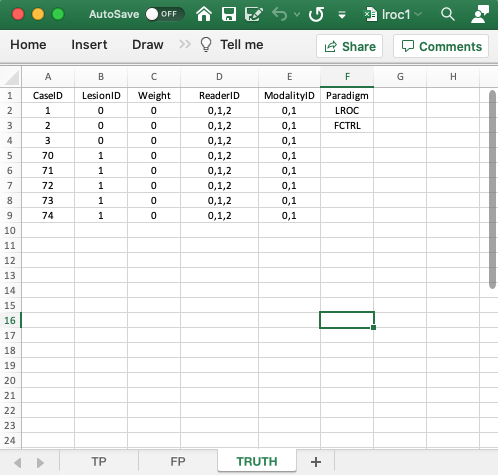
\includegraphics[width=1\textwidth,height=\textheight]{images/quick-start/lroc1Truth.png}

\begin{itemize}
\tightlist
\item
  The \texttt{Truth} worksheet is similar to that described previously for the ROC and LROC paradigms. The only difference is the first entry in the Paradigm column, which is \texttt{LROC}.
\item
  Since a diseased case has one lesion, the first five columns contain as many rows as there are cases in the dataset. There being 8 cases in the dataset, there are 8 rows of data.
\item
  \texttt{CaseID}: unique \textbf{integers} representing the cases in the dataset: `1', `2', `3', the 3 non-diseased cases, and `70', `71', `72', `73', `74', the 5 diseased cases.\\
\item
  \texttt{LesionID}: integers 0 or 1.

  \begin{itemize}
  \tightlist
  \item
    Each 0 represents a non-diseased case,
  \item
    Each 1 represents the solitary lesion in the diseased case.
  \end{itemize}
\item
  There are 3 non-diseased cases in the dataset (the number of 0's in the \texttt{LesionID} column).
\item
  There are 5 diseased cases in the dataset (the number of 1's in the \texttt{LesionID} column).
\item
  \texttt{Weight}: this column is filled with zeroes. With one lesion per case, the weights are irrelevant.
\item
  \texttt{ReaderID}: In the example shown each cell has the value `0, 1, 2'. There are 3 readers in the dataset, labeled \texttt{0}, \texttt{1} and \texttt{2}.
\item
  \texttt{ModalityID}: In the example each cell has the value \texttt{0,\ 1}. There are 2 modalities in the dataset, labeled \texttt{0} and \texttt{1}.
\item
  \texttt{Paradigm}: The contents are \texttt{LROC} and \texttt{FCTRL}: this is an \texttt{LROC} dataset and the design is ``factorial''.
\end{itemize}

\hypertarget{quick-start-lroc-tp1}{%
\section{\texorpdfstring{\texttt{TP} worksheet, forced localization true}{TP worksheet, forced localization true}}\label{quick-start-lroc-tp1}}

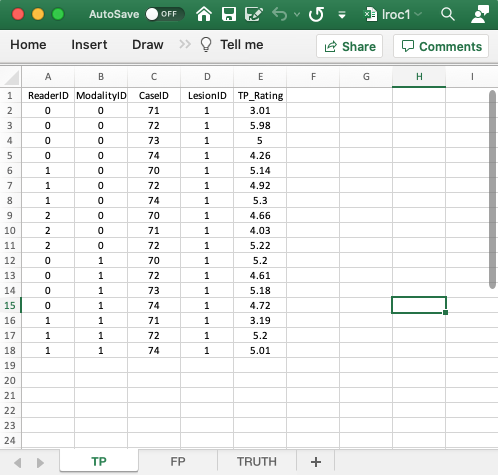
\includegraphics[width=1\textwidth,height=\textheight]{images/quick-start/lroc1TP.png}

\begin{itemize}
\tightlist
\item
  The \texttt{TP} worksheet is similar to that described previously for the ROC and FROC paradigms.
\item
  This worksheet can only have diseased cases. The presence of a non-diseased case in this worksheet will generate an error.
\item
  The key difference is that for each modality-reader and diseased-case combination there can be at most one entry. Also, if a particular combination is missing in the TP worksheet then it must appear in the FP worksheet. This is because this is a forced-mark-per-case dataset.
\item
  There can be at most 30 rows of data in this worksheet: 2 modalities times 3 readers times 5 diseased cases. Since there in fact only 17 rows of data, the missing 13 rows must occur in the FP worksheet.
\item
  Recall that each entry in the TP worksheet represents a correct localization while each missing entry represents an incorrect localization. The incorrect localizations are recorded in the FP worksheet.
\end{itemize}

\hypertarget{quick-start-lroc-fp1}{%
\section{\texorpdfstring{\texttt{FP} worksheet, forced localization true}{FP worksheet, forced localization true}}\label{quick-start-lroc-fp1}}

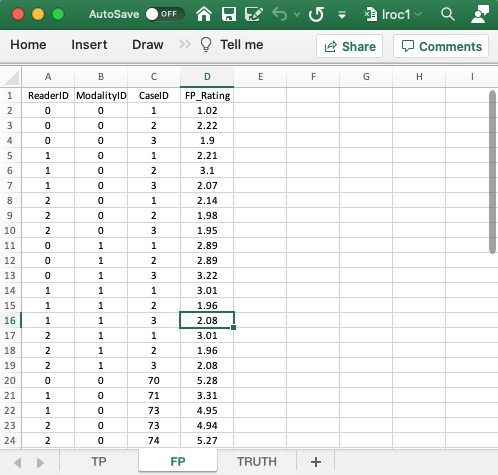
\includegraphics[width=1\textwidth,height=\textheight]{images/quick-start/lroc1FP1.png}

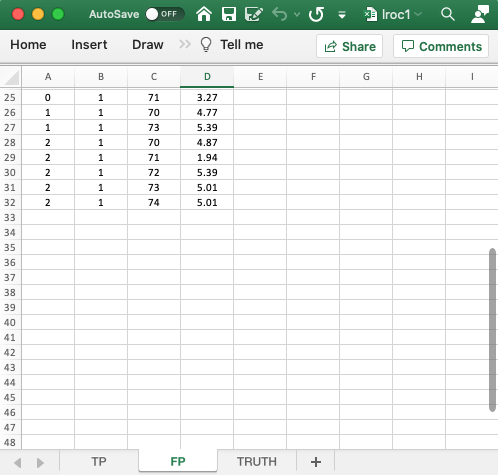
\includegraphics[width=1\textwidth,height=\textheight]{images/quick-start/lroc1FP2.png}

\begin{itemize}
\tightlist
\item
  The \texttt{FP} worksheet is similar to that described previously for the ROC and FROC paradigms.
\item
  Because of the forced mark requirement, there are 18 rows of data corresponding to non-diseased cases: 2 modalities times 3 readers times 3 non-diseased cases. The missing 13 rows from the TP worksheet are listed next; these correspond to the incorrect localizations on diseased cases. Therefore, the total number of rows in this worksheet is 18 + 13 = 31.
\item
  As an example, it is seen that for \texttt{modalityID} = 0 and \texttt{readerID} = 0, \texttt{caseID} = 70 does not appear in the TP worksheet. The lesion on this case was not localized; therefore it must appear in the FP worksheet as an incorrect localization, which is seen to be true in the FP worksheet.
\item
  As another example, for \texttt{modalityID} = 0 and \texttt{readerID} = 1, \texttt{caseID} = 71 does not appear in the TP worksheet; instead it appears in the FP worksheet.
\item
  As a final example, for \texttt{modalityID} = 1 and \texttt{readerID} = 2, none of the diseased cases appears in the TP worksheet; instead they all appear in the FP worksheet.
\end{itemize}

\hypertarget{quick-start-lroc-data-1}{%
\section{Reading forced localization true LROC dataset}\label{quick-start-lroc-data-1}}

The images shown above correspond to file \texttt{R/quick-start/lroc1.xlsx}. The next code chunk reads this file into an \texttt{R} object \texttt{x1}. Note the usage of the \texttt{lrocForcedMark} flag, which is set to \texttt{TRUE}, because this is a forced localization LROC dataset.

\begin{Shaded}
\begin{Highlighting}[]
\NormalTok{lroc1 <-}\StringTok{ "R/quick-start/lroc1.xlsx"}
\NormalTok{x1 <-}\StringTok{ }\KeywordTok{DfReadDataFile}\NormalTok{(lroc1, }\DataTypeTok{newExcelFileFormat =} \OtherTok{TRUE}\NormalTok{, }\DataTypeTok{lrocForcedMark =}\NormalTok{ T)}
\KeywordTok{str}\NormalTok{(x1)}
\CommentTok{#> List of 3}
\CommentTok{#>  $ ratings     :List of 3}
\CommentTok{#>   ..$ NL   : num [1:2, 1:3, 1:8, 1] 1.02 2.89 2.21 3.01 2.14 3.01 2.22 2.89 3.1 1.96 ...}
\CommentTok{#>   ..$ LL   : num [1:2, 1:3, 1:5, 1] -Inf 5.2 5.14 -Inf 4.66 ...}
\CommentTok{#>   ..$ LL_IL: num [1:2, 1:3, 1:5, 1] 5.28 -Inf -Inf 4.77 -Inf ...}
\CommentTok{#>  $ lesions     :List of 3}
\CommentTok{#>   ..$ perCase: int [1:5] 1 1 1 1 1}
\CommentTok{#>   ..$ IDs    : num [1:5, 1] 1 1 1 1 1}
\CommentTok{#>   ..$ weights: num [1:5, 1] 1 1 1 1 1}
\CommentTok{#>  $ descriptions:List of 7}
\CommentTok{#>   ..$ fileName     : chr "lroc1"}
\CommentTok{#>   ..$ type         : chr "LROC"}
\CommentTok{#>   ..$ name         : logi NA}
\CommentTok{#>   ..$ truthTableStr: num [1:2, 1:3, 1:8, 1:2] 1 1 1 1 1 1 1 1 1 1 ...}
\CommentTok{#>   ..$ design       : chr "FCTRL"}
\CommentTok{#>   ..$ modalityID   : Named chr [1:2] "0" "1"}
\CommentTok{#>   .. ..- attr(*, "names")= chr [1:2] "0" "1"}
\CommentTok{#>   ..$ readerID     : Named chr [1:3] "0" "1" "2"}
\CommentTok{#>   .. ..- attr(*, "names")= chr [1:3] "0" "1" "2"}
\end{Highlighting}
\end{Shaded}

This follows the general description in Chapter \ref{quick-start-data-format}. The differences are described below.

\begin{itemize}
\tightlist
\item
  \texttt{x1\$ratings\$NL} is a {[}2,3,8,1{]} dimension vector. For each modality and reader, only the first three elements, corresponding to the three non-diseased cases, are finite, the rest are \texttt{-Inf}.
\end{itemize}

For example:

\begin{Shaded}
\begin{Highlighting}[]
\NormalTok{x1}\OperatorTok{$}\NormalTok{ratings}\OperatorTok{$}\NormalTok{NL[}\DecValTok{1}\NormalTok{,}\DecValTok{1}\NormalTok{,,}\DecValTok{1}\NormalTok{]}
\CommentTok{#> [1] 1.02 2.22 1.90 -Inf -Inf -Inf -Inf -Inf}
\end{Highlighting}
\end{Shaded}

\begin{itemize}
\tightlist
\item
  x1\(ratings\)LL\texttt{is\ a\ {[}2,3,5,1{]}\ dimension\ vector.\ For\ each\ modality\ and\ reader,\ only\ the\ first\ three\ elements,\ corresponding\ to\ the\ three\ non-diseased\ cases,\ are\ finite,\ the\ rest\ are}-Inf`.
\end{itemize}

For example, since none of the lesions are localized for \texttt{modalityID} = 1 (second modality) and \texttt{readerID} = 2 (third reader), the following code yields a vector consisting of five \texttt{-Inf} values:

\begin{Shaded}
\begin{Highlighting}[]
\NormalTok{x1}\OperatorTok{$}\NormalTok{ratings}\OperatorTok{$}\NormalTok{LL[}\DecValTok{2}\NormalTok{,}\DecValTok{3}\NormalTok{,,}\DecValTok{1}\NormalTok{]}
\CommentTok{#> [1] -Inf -Inf -Inf -Inf -Inf}
\end{Highlighting}
\end{Shaded}

\begin{itemize}
\tightlist
\item
  \texttt{x1\$ratings\$LL\_IL} is a {[}2,3,5,1{]} dimension vector. These contain the ratings of incorrect localizations on diseased cases. For the just preceding modality-reader combination, this yields a vector with 5 finite values, the ratings of incorrect localizations for \texttt{modalityID} = 1 and \texttt{readerID} = 2.
\end{itemize}

\begin{Shaded}
\begin{Highlighting}[]
\NormalTok{x1}\OperatorTok{$}\NormalTok{ratings}\OperatorTok{$}\NormalTok{LL_IL[}\DecValTok{2}\NormalTok{,}\DecValTok{3}\NormalTok{,,}\DecValTok{1}\NormalTok{]}
\CommentTok{#> [1] 4.87 1.94 5.39 5.01 5.01}
\end{Highlighting}
\end{Shaded}

\hypertarget{quick-start-lroc-tp2}{%
\section{\texorpdfstring{\texttt{TP} worksheet, forced localization false}{TP worksheet, forced localization false}}\label{quick-start-lroc-tp2}}

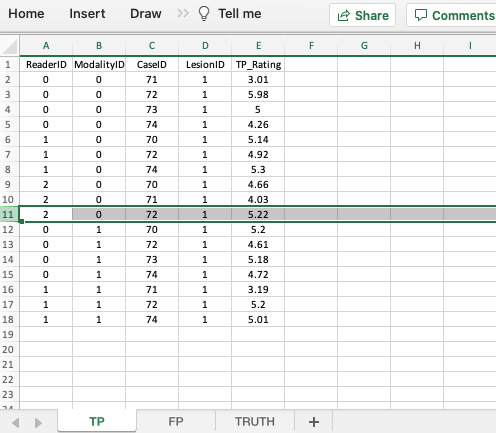
\includegraphics[width=1\textwidth,height=\textheight]{images/quick-start/lroc2TP.png}

\hypertarget{quick-start-lroc-fp2}{%
\section{\texorpdfstring{\texttt{FP} worksheet, forced localization false}{FP worksheet, forced localization false}}\label{quick-start-lroc-fp2}}

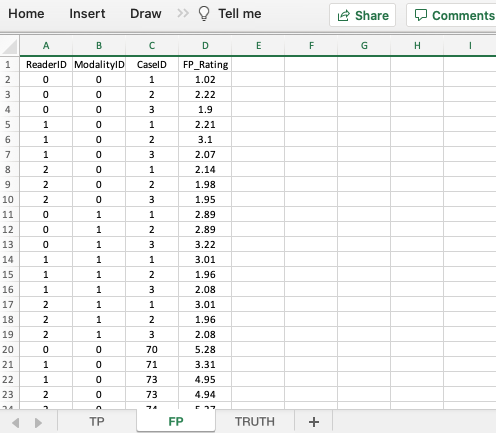
\includegraphics[width=1\textwidth,height=\textheight]{images/quick-start/lroc2FP1.png}

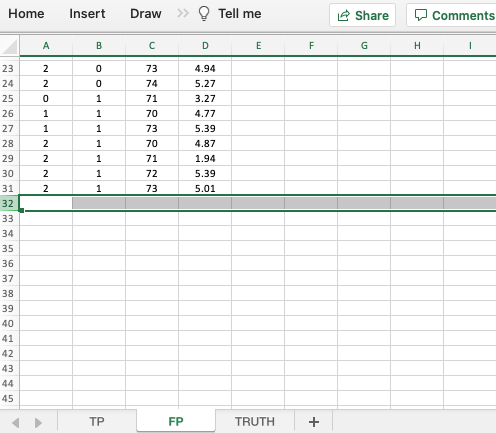
\includegraphics[width=1\textwidth,height=\textheight]{images/quick-start/lroc2FP2.png}

\begin{itemize}
\tightlist
\item
  If a particular modality-reader-case combination is missing in the TP worksheet then it need not appear in the FP worksheet. This is because this is not a forced-mark-per-case dataset.
\item
  As an example, \texttt{modalityID} = 1, \texttt{readerID} = 2 and \texttt{caseID} = 74 does not appear in either TP or FP worksheets.
\end{itemize}

\hypertarget{quick-start-lroc-data-2}{%
\section{Reading forced localization false LROC dataset}\label{quick-start-lroc-data-2}}

The next example is for file \texttt{R/quick-start/lroc2.xlsx}. The following code chunk reads this file into an \texttt{R} object \texttt{x2}. Note that for this dataset one must set the \texttt{lrocForcedMark} flag to \texttt{FALSE}, because this is \emph{not} a forced localization LROC dataset. Setting \texttt{lrocForcedMark} flag to \texttt{TRUE} will generate an error.

\begin{Shaded}
\begin{Highlighting}[]
\NormalTok{lroc2 <-}\StringTok{ "R/quick-start/lroc2.xlsx"}
\NormalTok{x2 <-}\StringTok{ }\KeywordTok{DfReadDataFile}\NormalTok{(lroc2, }\DataTypeTok{newExcelFileFormat =} \OtherTok{TRUE}\NormalTok{, }\DataTypeTok{lrocForcedMark =}\NormalTok{ F)}
\KeywordTok{str}\NormalTok{(x2)}
\CommentTok{#> List of 3}
\CommentTok{#>  $ ratings     :List of 3}
\CommentTok{#>   ..$ NL   : num [1:2, 1:3, 1:8, 1] 1.02 2.89 2.21 3.01 2.14 3.01 2.22 2.89 3.1 1.96 ...}
\CommentTok{#>   ..$ LL   : num [1:2, 1:3, 1:5, 1] -Inf 5.2 5.14 -Inf 4.66 ...}
\CommentTok{#>   ..$ LL_IL: num [1:2, 1:3, 1:5, 1] 5.28 -Inf -Inf 4.77 -Inf ...}
\CommentTok{#>  $ lesions     :List of 3}
\CommentTok{#>   ..$ perCase: int [1:5] 1 1 1 1 1}
\CommentTok{#>   ..$ IDs    : num [1:5, 1] 1 1 1 1 1}
\CommentTok{#>   ..$ weights: num [1:5, 1] 1 1 1 1 1}
\CommentTok{#>  $ descriptions:List of 7}
\CommentTok{#>   ..$ fileName     : chr "lroc2"}
\CommentTok{#>   ..$ type         : chr "LROC"}
\CommentTok{#>   ..$ name         : logi NA}
\CommentTok{#>   ..$ truthTableStr: num [1:2, 1:3, 1:8, 1:2] 1 1 1 1 1 1 1 1 1 1 ...}
\CommentTok{#>   ..$ design       : chr "FCTRL"}
\CommentTok{#>   ..$ modalityID   : Named chr [1:2] "0" "1"}
\CommentTok{#>   .. ..- attr(*, "names")= chr [1:2] "0" "1"}
\CommentTok{#>   ..$ readerID     : Named chr [1:3] "0" "1" "2"}
\CommentTok{#>   .. ..- attr(*, "names")= chr [1:3] "0" "1" "2"}
\end{Highlighting}
\end{Shaded}

\begin{itemize}
\tightlist
\item
  The \texttt{x2\$ratings\$LL} array is a {[}2,3,5,1{]} dimension vector. For each modality and reader, only the first three elements, corresponding to the three non-diseased cases, are finite, the rest are \texttt{-Inf}.
\end{itemize}

For example, since none of the lesions are localized for \texttt{modalityID} = 1 (second modality) and \texttt{readerID} = 2 (third reader), the following code yields a vector consisting of five \texttt{-Inf} values:

\begin{Shaded}
\begin{Highlighting}[]
\NormalTok{x2}\OperatorTok{$}\NormalTok{ratings}\OperatorTok{$}\NormalTok{LL[}\DecValTok{2}\NormalTok{,}\DecValTok{3}\NormalTok{,,}\DecValTok{1}\NormalTok{]}
\CommentTok{#> [1] -Inf -Inf -Inf -Inf -Inf}
\end{Highlighting}
\end{Shaded}

\begin{itemize}
\tightlist
\item
  The \texttt{x2\$ratings\$LL\_IL} is a {[}2,3,5,1{]} dimension vector. These contain the ratings of incorrect localizations on diseased cases. For the just preceding modality-reader combination, this yields a vector with 4 finite values, the ratings of incorrect localizations for \texttt{modalityID} = 1 and \texttt{readerID} = 2.
\end{itemize}

\begin{Shaded}
\begin{Highlighting}[]
\NormalTok{x2}\OperatorTok{$}\NormalTok{ratings}\OperatorTok{$}\NormalTok{LL_IL[}\DecValTok{2}\NormalTok{,}\DecValTok{3}\NormalTok{,,}\DecValTok{1}\NormalTok{]}
\CommentTok{#> [1] 4.87 1.94 5.39 5.01 -Inf}
\end{Highlighting}
\end{Shaded}

For this modality-reader combination case 74 (i.e., the fifth diseased case) was unmarked. It does not appear in either the TP or the FP worksheet.

\hypertarget{quick-start-lroc-data-summary}{%
\section{Summary}\label{quick-start-lroc-data-summary}}

The difference from the previous data structures is the existence of \texttt{LL\_IL} in the \texttt{ratings} list, which contains the ratings of incorrect localizations. Recall that for ROC and FROC paradigms this member was \texttt{NA}. When the data obeys forced localization, the corresponding flag should be set to \texttt{TRUE}, otherwise it should be set to \texttt{FALSE}. The default value of this flag is \texttt{NA}, which will work for ROC or FROC datasets. For LROC datasets it should be set to \texttt{T/F}.

\hypertarget{quick-start-lroc-data-references}{%
\section{References}\label{quick-start-lroc-data-references}}

\hypertarget{quick-start-dbm-text}{%
\chapter{DBM analysis text output}\label{quick-start-dbm-text}}

\hypertarget{quick-start-dbm-text-how-much-finished}{%
\section{TBA How much finished}\label{quick-start-dbm-text-how-much-finished}}

50\%

\hypertarget{quick-start-dbm-text-intro}{%
\section{Introduction}\label{quick-start-dbm-text-intro}}

This chapter illustrates significance testing using the DBM method.

\hypertarget{quick-start-dbm-text-analyze-dataset}{%
\section{Analyzing the ROC dataset}\label{quick-start-dbm-text-analyze-dataset}}

This illustrates the \texttt{StSignificanceTesting()} function. The significance testing method is specified as \texttt{"DBM"} and the figure of merit \texttt{FOM} is specified as ``Wilcoxon''. The embedded dataset \texttt{dataset03} is used.

\begin{Shaded}
\begin{Highlighting}[]
\NormalTok{ret <-}\StringTok{ }\KeywordTok{StSignificanceTesting}\NormalTok{(dataset03, }\DataTypeTok{FOM =} \StringTok{"Wilcoxon"}\NormalTok{, }\DataTypeTok{method =} \StringTok{"DBM"}\NormalTok{)}
\end{Highlighting}
\end{Shaded}

\hypertarget{quick-start-dbm-text-explanation}{%
\section{Explanation of the output}\label{quick-start-dbm-text-explanation}}

The function returns a list with 5 members:

\begin{itemize}
\tightlist
\item
  \texttt{FOMs}: figures of merit.
\item
  \texttt{ANOVA}: ANOVA tables.
\item
  \texttt{RRRC}: random-reader random-case analyses results.
\item
  \texttt{FRRC}: fixed-reader random-case analyses results.
\item
  \texttt{RRFC}" random-reader fixed-case analyses results.
\end{itemize}

Let us consider them individually.

\begin{Shaded}
\begin{Highlighting}[]
\KeywordTok{str}\NormalTok{(ret}\OperatorTok{$}\NormalTok{FOMs)}
\CommentTok{#> List of 3}
\CommentTok{#>  $ foms        :'data.frame':    2 obs. of  4 variables:}
\CommentTok{#>   ..$ rdrREADER_1: num [1:2] 0.853 0.85}
\CommentTok{#>   ..$ rdrREADER_2: num [1:2] 0.865 0.844}
\CommentTok{#>   ..$ rdrREADER_3: num [1:2] 0.857 0.84}
\CommentTok{#>   ..$ rdrREADER_4: num [1:2] 0.815 0.814}
\CommentTok{#>  $ trtMeans    :'data.frame':    2 obs. of  1 variable:}
\CommentTok{#>   ..$ Estimate: num [1:2] 0.848 0.837}
\CommentTok{#>  $ trtMeanDiffs:'data.frame':    1 obs. of  1 variable:}
\CommentTok{#>   ..$ Estimate: num 0.0109}
\end{Highlighting}
\end{Shaded}

\begin{itemize}
\tightlist
\item
  \texttt{FOMs} is a list of 3

  \begin{itemize}
  \tightlist
  \item
    \texttt{foms} is a {[}2x4{]} dataframe: the figure of merit for each of of the four observers in the two treatments.
  \item
    \texttt{trtMeans} is a {[}2x1{]} dataframe: the average figure of merit over all readers for each treatment.
  \item
    \texttt{trtMeanDiffs} a {[}1x1{]} dataframe: the difference(s) of the reader-averaged figures of merit for all different-treatment pairings. In this example, with only two treatments, there is only one different-treatment pairing.
  \end{itemize}
\end{itemize}

\begin{Shaded}
\begin{Highlighting}[]
\NormalTok{ret}\OperatorTok{$}\NormalTok{FOMs}\OperatorTok{$}\NormalTok{foms}
\CommentTok{#>           rdrREADER_1 rdrREADER_2 rdrREADER_3 rdrREADER_4}
\CommentTok{#> trtTREAT1  0.85345997  0.86499322  0.85730439  0.81524197}
\CommentTok{#> trtTREAT2  0.84961556  0.84350972  0.84011759  0.81433740}
\NormalTok{ret}\OperatorTok{$}\NormalTok{FOMs}\OperatorTok{$}\NormalTok{trtMeans}
\CommentTok{#>             Estimate}
\CommentTok{#> trtTREAT1 0.84774989}
\CommentTok{#> trtTREAT2 0.83689507}
\NormalTok{ret}\OperatorTok{$}\NormalTok{FOMs}\OperatorTok{$}\NormalTok{trtMeanDiffs}
\CommentTok{#>                        Estimate}
\CommentTok{#> trtTREAT1-trtTREAT2 0.010854817}
\end{Highlighting}
\end{Shaded}

\begin{Shaded}
\begin{Highlighting}[]
\KeywordTok{str}\NormalTok{(ret}\OperatorTok{$}\NormalTok{ANOVA)}
\CommentTok{#> List of 4}
\CommentTok{#>  $ TRCanova     :'data.frame':   8 obs. of  3 variables:}
\CommentTok{#>   ..$ SS: num [1:8] 0.0236 0.2052 52.5284 0.0151 6.41 ...}
\CommentTok{#>   ..$ DF: num [1:8] 1 3 99 3 99 297 297 799}
\CommentTok{#>   ..$ MS: num [1:8] 0.02357 0.06841 0.53059 0.00502 0.06475 ...}
\CommentTok{#>  $ VarCom       :'data.frame':   6 obs. of  1 variable:}
\CommentTok{#>   ..$ Estimates: num [1:6] 3.78e-05 5.13e-02 -7.13e-04 -2.89e-03 2.79e-02 ...}
\CommentTok{#>  $ IndividualTrt:'data.frame':   3 obs. of  3 variables:}
\CommentTok{#>   ..$ DF       : num [1:3] 3 99 297}
\CommentTok{#>   ..$ TrtTREAT1: num [1:3] 0.0493 0.294 0.105}
\CommentTok{#>   ..$ TrtTREAT2: num [1:3] 0.0242 0.3014 0.1034}
\CommentTok{#>  $ IndividualRdr:'data.frame':   3 obs. of  5 variables:}
\CommentTok{#>   ..$ DF         : num [1:3] 1 99 99}
\CommentTok{#>   ..$ rdrREADER_1: num [1:3] 0.000739 0.203875 0.091559}
\CommentTok{#>   ..$ rdrREADER_2: num [1:3] 0.0231 0.2234 0.0803}
\CommentTok{#>   ..$ rdrREADER_3: num [1:3] 0.0148 0.2142 0.0612}
\CommentTok{#>   ..$ rdrREADER_4: num [1:3] 4.09e-05 2.85e-01 6.06e-02}
\end{Highlighting}
\end{Shaded}

\begin{itemize}
\tightlist
\item
  ANOVA is a list of 4

  \begin{itemize}
  \tightlist
  \item
    \texttt{TRCanova} is a {[}8x3{]} dataframe: the treatment-reader-case ANOVA table, see below, where SS is the sum of squares, DF is the denominator degrees of freedom and MS is the mean squares, and T = treatment, R = reader, C = case, TR = treatment-reader, TC = treatment-case, RC = reader-case, TRC = treatment-reader-case.\\
  \item
    \texttt{VarCom} is a {[}6x1{]} dataframe: the variance components, see below, where \texttt{varR} is the reader variance, \texttt{varC} is the case variance, \texttt{varTR} is the treatment-reader variance, \texttt{varTC} is the treatment-case variance, \texttt{varRC} is the reader-case variance, and \texttt{varTRC} is the treatment-reader-case variance.
  \item
    \texttt{IndividualTrt} is a {[}3x3{]} dataframe: the individual treatment variance components averaged over all readers, see below, where \texttt{msR} is the mean square reader, \texttt{msC} is the mean square case and \texttt{msRC} is the mean square reader-case.
  \item
    \texttt{IndividualRdr} is a {[}3x5{]} dataframe: the individual reader variance components averaged over treatments, see below, where \texttt{msT} is the mean square treatment, \texttt{msC} is the mean square case and \texttt{msTC} is the mean square treatment-case.
  \end{itemize}
\end{itemize}

\begin{Shaded}
\begin{Highlighting}[]
\NormalTok{ret}\OperatorTok{$}\NormalTok{ANOVA}\OperatorTok{$}\NormalTok{TRCanova}
\CommentTok{#>                  SS  DF           MS}
\CommentTok{#> T       0.023565410   1 0.0235654097}
\CommentTok{#> R       0.205217999   3 0.0684059998}
\CommentTok{#> C      52.528398680  99 0.5305898857}
\CommentTok{#> TR      0.015060792   3 0.0050202641}
\CommentTok{#> TC      6.410048814  99 0.0647479678}
\CommentTok{#> RC     39.242953812 297 0.1321311576}
\CommentTok{#> TRC    22.660077641 297 0.0762965577}
\CommentTok{#> Total 121.085323149 799           NA}
\NormalTok{ret}\OperatorTok{$}\NormalTok{ANOVA}\OperatorTok{$}\NormalTok{VarCom}
\CommentTok{#>             Estimates}
\CommentTok{#> VarR    3.7755679e-05}
\CommentTok{#> VarC    5.1250915e-02}
\CommentTok{#> VarTR  -7.1276294e-04}
\CommentTok{#> VarTC  -2.8871475e-03}
\CommentTok{#> VarRC   2.7917300e-02}
\CommentTok{#> VarErr  7.6296558e-02}
\NormalTok{ret}\OperatorTok{$}\NormalTok{ANOVA}\OperatorTok{$}\NormalTok{IndividualTrt}
\CommentTok{#>       DF   TrtTREAT1   TrtTREAT2}
\CommentTok{#> msR    3 0.049266349 0.024159915}
\CommentTok{#> msC   99 0.293967531 0.301370323}
\CommentTok{#> msRC 297 0.105047872 0.103379843}
\NormalTok{ret}\OperatorTok{$}\NormalTok{ANOVA}\OperatorTok{$}\NormalTok{IndividualRdr}
\CommentTok{#>      DF   rdrREADER_1 rdrREADER_2 rdrREADER_3   rdrREADER_4}
\CommentTok{#> msT   1 0.00073897606 0.023077021 0.014769293 0.00004091217}
\CommentTok{#> msC  99 0.20387477465 0.223441908 0.214246773 0.28541990211}
\CommentTok{#> msTC 99 0.09155873437 0.080279256 0.061228980 0.06057067104}
\end{Highlighting}
\end{Shaded}

\begin{Shaded}
\begin{Highlighting}[]
\KeywordTok{str}\NormalTok{(ret}\OperatorTok{$}\NormalTok{RRRC)}
\CommentTok{#> List of 3}
\CommentTok{#>  $ FTests         :'data.frame': 2 obs. of  4 variables:}
\CommentTok{#>   ..$ DF   : num [1:2] 1 3}
\CommentTok{#>   ..$ MS   : num [1:2] 0.02357 0.00502}
\CommentTok{#>   ..$ FStat: num [1:2] 4.69 NA}
\CommentTok{#>   ..$ p    : num [1:2] 0.119 NA}
\CommentTok{#>  $ ciDiffTrt      :'data.frame': 1 obs. of  7 variables:}
\CommentTok{#>   ..$ Estimate: num 0.0109}
\CommentTok{#>   ..$ StdErr  : num 0.00501}
\CommentTok{#>   ..$ DF      : num 3}
\CommentTok{#>   ..$ t       : num 2.17}
\CommentTok{#>   ..$ PrGTt   : num 0.119}
\CommentTok{#>   ..$ CILower : num -0.00509}
\CommentTok{#>   ..$ CIUpper : num 0.0268}
\CommentTok{#>  $ ciAvgRdrEachTrt:'data.frame': 2 obs. of  5 variables:}
\CommentTok{#>   ..$ Estimate: num [1:2] 0.848 0.837}
\CommentTok{#>   ..$ StdErr  : num [1:2] 0.0244 0.0236}
\CommentTok{#>   ..$ DF      : num [1:2] 70.1 253.6}
\CommentTok{#>   ..$ CILower : num [1:2] 0.799 0.79}
\CommentTok{#>   ..$ CIUpper : num [1:2] 0.896 0.883}
\end{Highlighting}
\end{Shaded}

\begin{itemize}
\tightlist
\item
  RRRC, a list of 3 containing results of random-reader random-case analyses

  \begin{itemize}
  \tightlist
  \item
    \texttt{FTtests}: is a {[}2x4{]} dataframe: results of the F-tests, see below, where \texttt{FStat} is the F-statistic and \texttt{p} is the p-value. The first row is the treatment effect and the second is the error term.
  \item
    \texttt{ciDiffTrt}: is a {[}1x7{]} dataframe: the confidence intervals between different-treatments, see below, where \texttt{StdErr} is the standard error of the estimate, \texttt{t} is the t-statistic and \texttt{PrGTt} is the p-value.
  \item
    \texttt{ciAvgRdrEachTrt}: is a {[}2x5{]} dataframe: the confidence intervals for each treatment, averaged over all readers in the treatment, see below, where \texttt{CILower} is the lower 95\% confidence interval and \texttt{CIUpper} is the upper 95\% confidence interval.
  \end{itemize}
\end{itemize}

\begin{Shaded}
\begin{Highlighting}[]
\NormalTok{ret}\OperatorTok{$}\NormalTok{RRRC}\OperatorTok{$}\NormalTok{FTests}
\CommentTok{#>           DF           MS     FStat          p}
\CommentTok{#> Treatment  1 0.0235654097 4.6940577 0.11883786}
\CommentTok{#> Error      3 0.0050202641        NA         NA}
\NormalTok{ret}\OperatorTok{$}\NormalTok{RRRC}\OperatorTok{$}\NormalTok{ciDiffTrt}
\CommentTok{#>                        Estimate       StdErr DF         t      PrGTt}
\CommentTok{#> trtTREAT1-trtTREAT2 0.010854817 0.0050101218  3 2.1665774 0.11883786}
\CommentTok{#>                           CILower     CIUpper}
\CommentTok{#> trtTREAT1-trtTREAT2 -0.0050896269 0.026799261}
\NormalTok{ret}\OperatorTok{$}\NormalTok{RRRC}\OperatorTok{$}\NormalTok{ciAvgRdrEachTrt}
\CommentTok{#>             Estimate      StdErr         DF    CILower    CIUpper}
\CommentTok{#> trtTREAT1 0.84774989 0.024402152  70.121788 0.79908282 0.89641696}
\CommentTok{#> trtTREAT2 0.83689507 0.023566416 253.644028 0.79048429 0.88330585}
\end{Highlighting}
\end{Shaded}

\begin{Shaded}
\begin{Highlighting}[]
\KeywordTok{str}\NormalTok{(ret}\OperatorTok{$}\NormalTok{FRRC)}
\CommentTok{#> List of 4}
\CommentTok{#>  $ FTests          :'data.frame':    2 obs. of  4 variables:}
\CommentTok{#>   ..$ DF   : num [1:2] 1 99}
\CommentTok{#>   ..$ MS   : num [1:2] 0.0236 0.0647}
\CommentTok{#>   ..$ FStat: num [1:2] 0.364 NA}
\CommentTok{#>   ..$ p    : num [1:2] 0.548 NA}
\CommentTok{#>  $ ciDiffTrt       :'data.frame':    1 obs. of  7 variables:}
\CommentTok{#>   ..$ Estimate: num 0.0109}
\CommentTok{#>   ..$ StdErr  : num 0.018}
\CommentTok{#>   ..$ DF      : num 99}
\CommentTok{#>   ..$ t       : num 0.603}
\CommentTok{#>   ..$ PrGTt   : num 0.548}
\CommentTok{#>   ..$ CILower : num -0.0248}
\CommentTok{#>   ..$ CIUpper : num 0.0466}
\CommentTok{#>  $ ciAvgRdrEachTrt :'data.frame':    2 obs. of  5 variables:}
\CommentTok{#>   ..$ Estimate: num [1:2] 0.848 0.837}
\CommentTok{#>   ..$ StdErr  : num [1:2] 0.0271 0.0274}
\CommentTok{#>   ..$ DF      : num [1:2] 99 99}
\CommentTok{#>   ..$ CILower : num [1:2] 0.794 0.782}
\CommentTok{#>   ..$ CIUpper : num [1:2] 0.902 0.891}
\CommentTok{#>  $ ciDiffTrtEachRdr:'data.frame':    4 obs. of  7 variables:}
\CommentTok{#>   ..$ Estimate: num [1:4] 0.003844 0.021483 0.017187 0.000905}
\CommentTok{#>   ..$ StdErr  : num [1:4] 0.0428 0.0401 0.035 0.0348}
\CommentTok{#>   ..$ DF      : num [1:4] 99 99 99 99}
\CommentTok{#>   ..$ t       : num [1:4] 0.0898 0.5362 0.4911 0.026}
\CommentTok{#>   ..$ PrGTt   : num [1:4] 0.929 0.593 0.624 0.979}
\CommentTok{#>   ..$ CILower : num [1:4] -0.0811 -0.058 -0.0522 -0.0682}
\CommentTok{#>   ..$ CIUpper : num [1:4] 0.0888 0.101 0.0866 0.07}
\end{Highlighting}
\end{Shaded}

\begin{itemize}
\tightlist
\item
  FRRC, a list of 4 containing results of fixed-reader random-case analyses

  \begin{itemize}
  \tightlist
  \item
    \texttt{FTtests}: is a {[}2x4{]} dataframe: results of the F-tests, see below.
  \item
    \texttt{ciDiffTrt}: is a {[}1x7{]} dataframe: the confidence intervals between different-treatments, see below.
  \item
    \texttt{ciAvgRdrEachTrt}: is a {[}2x5{]} dataframe: the confidence intervals for the average reader over each treatment
  \item
    \texttt{ciDiffTrtEachRdr}: is a {[}4x7{]} dataframe: the confidence intervals for each different-treatment pairing for each reader.
  \end{itemize}
\end{itemize}

\begin{Shaded}
\begin{Highlighting}[]
\NormalTok{ret}\OperatorTok{$}\NormalTok{FRRC}\OperatorTok{$}\NormalTok{FTests}
\CommentTok{#>           DF          MS      FStat          p}
\CommentTok{#> Treatment  1 0.023565410 0.36395597 0.54769704}
\CommentTok{#> Error     99 0.064747968         NA         NA}
\NormalTok{ret}\OperatorTok{$}\NormalTok{FRRC}\OperatorTok{$}\NormalTok{ciDiffTrt}
\CommentTok{#>                        Estimate      StdErr DF          t      PrGTt}
\CommentTok{#> trtTREAT1-trtTREAT2 0.010854817 0.017992772 99 0.60328764 0.54769704}
\CommentTok{#>                          CILower    CIUpper}
\CommentTok{#> trtTREAT1-trtTREAT2 -0.024846746 0.04655638}
\NormalTok{ret}\OperatorTok{$}\NormalTok{FRRC}\OperatorTok{$}\NormalTok{ciAvgRdrEachTrt}
\CommentTok{#>             Estimate      StdErr DF    CILower    CIUpper}
\CommentTok{#> trtTREAT1 0.84774989 0.027109386 99 0.79395898 0.90154079}
\CommentTok{#> trtTREAT2 0.83689507 0.027448603 99 0.78243109 0.89135905}
\NormalTok{ret}\OperatorTok{$}\NormalTok{FRRC}\OperatorTok{$}\NormalTok{ciDiffTrtEachRdr}
\CommentTok{#>                                       Estimate      StdErr DF           t}
\CommentTok{#> rdrREADER_1::trtTREAT1-trtTREAT2 0.00384441429 0.042792227 99 0.089839080}
\CommentTok{#> rdrREADER_2::trtTREAT1-trtTREAT2 0.02148349163 0.040069753 99 0.536152334}
\CommentTok{#> rdrREADER_3::trtTREAT1-trtTREAT2 0.01718679331 0.034993994 99 0.491135520}
\CommentTok{#> rdrREADER_4::trtTREAT1-trtTREAT2 0.00090456807 0.034805365 99 0.025989329}
\CommentTok{#>                                       PrGTt      CILower     CIUpper}
\CommentTok{#> rdrREADER_1::trtTREAT1-trtTREAT2 0.92859660 -0.081064648 0.088753476}
\CommentTok{#> rdrREADER_2::trtTREAT1-trtTREAT2 0.59305592 -0.058023592 0.100990575}
\CommentTok{#> rdrREADER_3::trtTREAT1-trtTREAT2 0.62441761 -0.052248882 0.086622469}
\CommentTok{#> rdrREADER_4::trtTREAT1-trtTREAT2 0.97931817 -0.068156827 0.069965963}
\end{Highlighting}
\end{Shaded}

\begin{Shaded}
\begin{Highlighting}[]
\KeywordTok{str}\NormalTok{(ret}\OperatorTok{$}\NormalTok{RRFC)}
\CommentTok{#> List of 3}
\CommentTok{#>  $ FTests         :'data.frame': 2 obs. of  4 variables:}
\CommentTok{#>   ..$ DF   : num [1:2] 1 3}
\CommentTok{#>   ..$ MS   : num [1:2] 0.02357 0.00502}
\CommentTok{#>   ..$ FStat: num [1:2] 4.69 NA}
\CommentTok{#>   ..$ p    : num [1:2] 0.119 NA}
\CommentTok{#>  $ ciDiffTrt      :'data.frame': 1 obs. of  7 variables:}
\CommentTok{#>   ..$ Estimate: num 0.0109}
\CommentTok{#>   ..$ StdErr  : num 0.00501}
\CommentTok{#>   ..$ DF      : num 3}
\CommentTok{#>   ..$ t       : num 2.17}
\CommentTok{#>   ..$ PrGTt   : num 0.119}
\CommentTok{#>   ..$ CILower : num -0.00509}
\CommentTok{#>   ..$ CIUpper : num 0.0268}
\CommentTok{#>  $ ciAvgRdrEachTrt:'data.frame': 2 obs. of  5 variables:}
\CommentTok{#>   ..$ Estimate: num [1:2] 0.848 0.837}
\CommentTok{#>   ..$ StdErr  : num [1:2] 0.0111 0.00777}
\CommentTok{#>   ..$ DF      : num [1:2] 3 3}
\CommentTok{#>   ..$ CILower : num [1:2] 0.812 0.812}
\CommentTok{#>   ..$ CIUpper : num [1:2] 0.883 0.862}
\end{Highlighting}
\end{Shaded}

\begin{itemize}
\tightlist
\item
  RRFC, a list of 3 containing results of random-reader fixed-case analyses

  \begin{itemize}
  \tightlist
  \item
    \texttt{FTtests}: is a {[}2x4{]} dataframe: results of the F-tests, see below.
  \item
    \texttt{ciDiffTrt}: is a {[}1x7{]} dataframe: the confidence intervals between different-treatments, see below.
  \item
    \texttt{ciAvgRdrEachTrt}: is a {[}2x5{]} dataframe: the confidence intervals for the average reader over each over each treatment.
  \end{itemize}
\end{itemize}

\begin{Shaded}
\begin{Highlighting}[]
\NormalTok{ret}\OperatorTok{$}\NormalTok{RRFC}\OperatorTok{$}\NormalTok{FTests}
\CommentTok{#>           DF           MS     FStat          p}
\CommentTok{#> Treatment  1 0.0235654097 4.6940577 0.11883786}
\CommentTok{#> Error      3 0.0050202641        NA         NA}
\NormalTok{ret}\OperatorTok{$}\NormalTok{RRFC}\OperatorTok{$}\NormalTok{ciDiffTrt}
\CommentTok{#>                        Estimate       StdErr DF         t      PrGTt}
\CommentTok{#> trtTREAT1-trtTREAT2 0.010854817 0.0050101218  3 2.1665774 0.11883786}
\CommentTok{#>                           CILower     CIUpper}
\CommentTok{#> trtTREAT1-trtTREAT2 -0.0050896269 0.026799261}
\NormalTok{ret}\OperatorTok{$}\NormalTok{RRFC}\OperatorTok{$}\NormalTok{ciAvgRdrEachTrt}
\CommentTok{#>             Estimate      StdErr DF    CILower    CIUpper}
\CommentTok{#> trtTREAT1 0.84774989 0.011098012  3 0.81243106 0.88306871}
\CommentTok{#> trtTREAT2 0.83689507 0.007771730  3 0.81216196 0.86162818}
\end{Highlighting}
\end{Shaded}

\hypertarget{quick-start-dbm-text-references}{%
\section{References}\label{quick-start-dbm-text-references}}

\hypertarget{quick-start-or-text}{%
\chapter{OR analysis text output}\label{quick-start-or-text}}

\hypertarget{quick-start-or-text-how-much-finished}{%
\section{TBA How much finished}\label{quick-start-or-text-how-much-finished}}

90\%

\hypertarget{quick-start-or-text-intro}{%
\section{Introduction}\label{quick-start-or-text-intro}}

This chapter illustrates significance testing using the DBM and OR methods.

\hypertarget{quick-start-or-text-analyze-dataset}{%
\section{Analyzing the ROC dataset}\label{quick-start-or-text-analyze-dataset}}

The only change is to specify \texttt{method\ =\ "OR"} in the significance testing function. The same dataset is used as was used in the previous chapter.

\begin{Shaded}
\begin{Highlighting}[]
\NormalTok{ret <-}\StringTok{ }\KeywordTok{StSignificanceTesting}\NormalTok{(dataset03, }\DataTypeTok{FOM =} \StringTok{"Wilcoxon"}\NormalTok{, }\DataTypeTok{method =} \StringTok{"OR"}\NormalTok{)}
\end{Highlighting}
\end{Shaded}

\hypertarget{quick-start-or-text-explanation}{%
\section{Explanation of the output}\label{quick-start-or-text-explanation}}

The function returns a list with 5 members.

\begin{itemize}
\tightlist
\item
  \texttt{FOMs}: figures of merit, identical to that in the DBM method.
\item
  \texttt{ANOVA}: ANOVA tables.
\item
  \texttt{RRRC}: random-reader random-case analyses results.
\item
  \texttt{FRRC}: fixed-reader random-case analyses results.
\item
  \texttt{RRFC}" random-reader fixed-case analyses results.
\end{itemize}

Let us consider the ones that are different from the DBM method.

\begin{itemize}
\tightlist
\item
  ANOVA is a list of 4

  \begin{itemize}
  \tightlist
  \item
    \texttt{TRanova} is a {[}3x3{]} dataframe: the treatment-reader ANOVA table, see below, where SS is the sum of squares, DF is the denominator degrees of freedom and MS is the mean squares, and T = treatment, R = reader, TR = treatment-reader.\\
  \item
    \texttt{VarCom} is a {[}6x2{]} dataframe: the variance components, see below, where \texttt{varR} is the reader variance, \texttt{varTR} is the treatment-reader variance, \texttt{Cov1}, \texttt{Cov2},\texttt{Cov3} and \texttt{Var} are as defined in the OR model. The second column lists the correlations defined in the OR model.
  \item
    \texttt{IndividualTrt} is a {[}2x4{]} dataframe: the individual treatment mean-squares, variances and \(Cov_2\), averaged over all readers, see below, where \texttt{msREachTrt} is the mean square reader, \texttt{varEachTrt} is the variance and \texttt{cov2EachTrt} is \texttt{Cov2EachTrt} in each treatment.
  \item
    \texttt{IndividualRdr} is a {[}2x4{]} dataframe: the individual reader variance components averaged over treatments, see below, where \texttt{msTEachRdr} is the mean square treatment, \texttt{varEachRdr} is the variance and \texttt{cov1EachRdr} is \(Cov_1\) for each reader.
  \end{itemize}
\end{itemize}

\begin{Shaded}
\begin{Highlighting}[]
\NormalTok{ret}\OperatorTok{$}\NormalTok{ANOVA}\OperatorTok{$}\NormalTok{TRanova}
\CommentTok{#>               SS DF            MS}
\CommentTok{#> T  0.00023565410  1 2.3565410e-04}
\CommentTok{#> R  0.00205217999  3 6.8406000e-04}
\CommentTok{#> TR 0.00015060792  3 5.0202641e-05}
\NormalTok{ret}\OperatorTok{$}\NormalTok{ANOVA}\OperatorTok{$}\NormalTok{VarCom}
\CommentTok{#>            Estimates       Rhos}
\CommentTok{#> VarR   2.3319942e-05         NA}
\CommentTok{#> VarTR -6.8389146e-04         NA}
\CommentTok{#> Cov1   7.9168215e-04 0.51887172}
\CommentTok{#> Cov2   4.8363767e-04 0.31697811}
\CommentTok{#> Cov3   5.1250915e-04 0.33590059}
\CommentTok{#> Var    1.5257762e-03         NA}
\NormalTok{ret}\OperatorTok{$}\NormalTok{ANOVA}\OperatorTok{$}\NormalTok{IndividualTrt}
\CommentTok{#>           DF    msREachTrt   varEachTrt   cov2EachTrt}
\CommentTok{#> trtTREAT1  3 0.00049266349 0.0015227779 0.00047229915}
\CommentTok{#> trtTREAT2  3 0.00024159915 0.0015287746 0.00049497620}
\NormalTok{ret}\OperatorTok{$}\NormalTok{ANOVA}\OperatorTok{$}\NormalTok{IndividualRdr}
\CommentTok{#>             DF    msTEachRdr   varEachRdr   cov1EachRdr}
\CommentTok{#> rdrREADER_1  1 7.3897606e-06 0.0014771675 0.00056158020}
\CommentTok{#> rdrREADER_2  1 2.3077021e-04 0.0015186058 0.00071581326}
\CommentTok{#> rdrREADER_3  1 1.4769293e-04 0.0013773788 0.00076508897}
\CommentTok{#> rdrREADER_4  1 4.0912170e-07 0.0017299529 0.00112424616}
\end{Highlighting}
\end{Shaded}

\begin{itemize}
\tightlist
\item
  RRRC, a list of 3 containing results of random-reader random-case analyses

  \begin{itemize}
  \tightlist
  \item
    \texttt{FTtests}: is a {[}2x4{]} dataframe: results of the F-tests, see below, where \texttt{FStat} is the F-statistic and \texttt{p} is the p-value. The first row is the treatment effect and the second is the error term.
  \item
    \texttt{ciDiffTrt}: is a {[}1x7{]} dataframe: the confidence intervals between different treatments, see below, where \texttt{StdErr} is the standard error of the estimate, \texttt{t} is the t-statistic and \texttt{PrGTt} is the p-value.
  \item
    \texttt{ciAvgRdrEachTrt}: is a {[}2x5{]} dataframe: the confidence intervals for the average reader over each treatment, see below, where \texttt{CILower} is the lower 95\% confidence interval and \texttt{CIUpper} is the upper 95\% confidence interval.
  \end{itemize}
\end{itemize}

\begin{Shaded}
\begin{Highlighting}[]
\NormalTok{ret}\OperatorTok{$}\NormalTok{RRRC}\OperatorTok{$}\NormalTok{FTests}
\CommentTok{#>           DF            MS     FStat          p}
\CommentTok{#> Treatment  1 2.3565410e-04 4.6940577 0.11883786}
\CommentTok{#> Error      3 5.0202641e-05        NA         NA}
\NormalTok{ret}\OperatorTok{$}\NormalTok{RRRC}\OperatorTok{$}\NormalTok{ciDiffTrt}
\CommentTok{#>                        Estimate       StdErr DF         t      PrGTt}
\CommentTok{#> trtTREAT1-trtTREAT2 0.010854817 0.0050101218  3 2.1665774 0.11883786}
\CommentTok{#>                           CILower     CIUpper}
\CommentTok{#> trtTREAT1-trtTREAT2 -0.0050896269 0.026799261}
\NormalTok{ret}\OperatorTok{$}\NormalTok{RRRC}\OperatorTok{$}\NormalTok{ciAvgRdrEachTrt}
\CommentTok{#>             Estimate      StdErr         DF    CILower    CIUpper          Cov2}
\CommentTok{#> trtTREAT1 0.84774989 0.024402152  70.121788 0.79908282 0.89641696 0.00047229915}
\CommentTok{#> trtTREAT2 0.83689507 0.023566416 253.644028 0.79048429 0.88330585 0.00049497620}
\end{Highlighting}
\end{Shaded}

\begin{itemize}
\tightlist
\item
  FRRC, a list of 5 containing results of fixed-reader random-case analyses

  \begin{itemize}
  \tightlist
  \item
    \texttt{FTtests}: is a {[}2x4{]} dataframe: results of the chisquare-tests, see below. Here is a difference from DBM: in the OR method for FRRC the denominator degrees of freedom of the F-statistic is infinite, and the test becomes equivalent to a chisquare test with the degrees of freedom equal to \(I-1\), where \(I\) is the number of treatments.
  \item
    \texttt{ciDiffTrt}: is a {[}1x6{]} dataframe: the confidence intervals between different treatments, see below. An additional column lists
  \item
    \texttt{ciAvgRdrEachTrt}: is a {[}2x5{]} dataframe: the confidence intervals for the average reader over each treatment
  \item
    \texttt{ciDiffTrtEachRdr}: is a {[}4x6{]} dataframe: the confidence intervals for each different-treatment pairing for each reader.
  \item
    \texttt{IndividualRdrVarCov1}: is a {[}4x2{]} dataframe: \(Var\) and \(Cov_1\) for individual readers.
  \end{itemize}
\end{itemize}

\begin{Shaded}
\begin{Highlighting}[]
\NormalTok{ret}\OperatorTok{$}\NormalTok{FRRC}\OperatorTok{$}\NormalTok{FTests}
\CommentTok{#>                     MS      Chisq DF          p}
\CommentTok{#> Treatment 0.0002356541 0.32101347  1 0.57099922}
\CommentTok{#> Error     0.0007340941         NA NA         NA}
\NormalTok{ret}\OperatorTok{$}\NormalTok{FRRC}\OperatorTok{$}\NormalTok{ciDiffTrt}
\CommentTok{#>                        Estimate      StdErr          z      PrGTz      CILower}
\CommentTok{#> trtTREAT1-trtTREAT2 0.010854817 0.019158472 0.56658051 0.57099922 -0.026695098}
\CommentTok{#>                         CIUpper}
\CommentTok{#> trtTREAT1-trtTREAT2 0.048404732}
\NormalTok{ret}\OperatorTok{$}\NormalTok{FRRC}\OperatorTok{$}\NormalTok{ciAvgRdrEachTrt}
\CommentTok{#>             Estimate      StdErr DF    CILower    CIUpper}
\CommentTok{#> trtTREAT1 0.84774989 0.027109386 99 0.79461647 0.90088331}
\CommentTok{#> trtTREAT2 0.83689507 0.027448603 99 0.78309680 0.89069334}
\NormalTok{ret}\OperatorTok{$}\NormalTok{FRRC}\OperatorTok{$}\NormalTok{ciDiffTrtEachRdr}
\CommentTok{#>                                       Estimate      StdErr           z}
\CommentTok{#> rdrREADER_1::trtTREAT1-trtTREAT2 0.00384441429 0.042792227 0.089839080}
\CommentTok{#> rdrREADER_2::trtTREAT1-trtTREAT2 0.02148349163 0.040069753 0.536152334}
\CommentTok{#> rdrREADER_3::trtTREAT1-trtTREAT2 0.01718679331 0.034993994 0.491135520}
\CommentTok{#> rdrREADER_4::trtTREAT1-trtTREAT2 0.00090456807 0.034805365 0.025989329}
\CommentTok{#>                                       PrGTz      CILower     CIUpper}
\CommentTok{#> rdrREADER_1::trtTREAT1-trtTREAT2 0.92841509 -0.080026809 0.087715638}
\CommentTok{#> rdrREADER_2::trtTREAT1-trtTREAT2 0.59185327 -0.057051781 0.100018765}
\CommentTok{#> rdrREADER_3::trtTREAT1-trtTREAT2 0.62333060 -0.051400174 0.085773761}
\CommentTok{#> rdrREADER_4::trtTREAT1-trtTREAT2 0.97926585 -0.067312693 0.069121830}
\NormalTok{ret}\OperatorTok{$}\NormalTok{FRRC}\OperatorTok{$}\NormalTok{IndividualRdrVarCov1}
\CommentTok{#>               varEachRdr   cov1EachRdr}
\CommentTok{#> rdrREADER_1 0.0014771675 0.00056158020}
\CommentTok{#> rdrREADER_2 0.0015186058 0.00071581326}
\CommentTok{#> rdrREADER_3 0.0013773788 0.00076508897}
\CommentTok{#> rdrREADER_4 0.0017299529 0.00112424616}
\end{Highlighting}
\end{Shaded}

\begin{itemize}
\tightlist
\item
  RRFC, a list of 3 containing results of random-reader fixed-case analyses

  \begin{itemize}
  \tightlist
  \item
    \texttt{FTtests}: is a {[}2x4{]} dataframe: results of the F-tests, see below.
  \item
    \texttt{ciDiffTrt}: is a {[}1x7{]} dataframe: the confidence intervals between different treatments, see below.
  \item
    \texttt{ciAvgRdrEachTrt}: is a {[}2x5{]} dataframe: the confidence intervals for the average reader over each over each treatment.
  \end{itemize}
\end{itemize}

\begin{Shaded}
\begin{Highlighting}[]
\NormalTok{ret}\OperatorTok{$}\NormalTok{RRFC}\OperatorTok{$}\NormalTok{FTests}
\CommentTok{#>    DF            MS         F          p}
\CommentTok{#> T   1 2.3565410e-04 4.6940577 0.11883786}
\CommentTok{#> TR  3 5.0202641e-05        NA         NA}
\NormalTok{ret}\OperatorTok{$}\NormalTok{RRFC}\OperatorTok{$}\NormalTok{ciDiffTrt}
\CommentTok{#>                        Estimate       StdErr DF         t      PrGTt}
\CommentTok{#> trtTREAT1-trtTREAT2 0.010854817 0.0050101218  3 2.1665774 0.11883786}
\CommentTok{#>                           CILower     CIUpper}
\CommentTok{#> trtTREAT1-trtTREAT2 -0.0050896269 0.026799261}
\NormalTok{ret}\OperatorTok{$}\NormalTok{RRFC}\OperatorTok{$}\NormalTok{ciAvgRdrEachTrt}
\CommentTok{#>             Estimate      StdErr DF    CILower    CIUpper}
\CommentTok{#> TrtTREAT1 0.84774989 0.011098012  3 0.81243106 0.88306871}
\CommentTok{#> TrtTREAT2 0.83689507 0.007771730  3 0.81216196 0.86162818}
\end{Highlighting}
\end{Shaded}

\hypertarget{quick-start-or-text-references}{%
\section{References}\label{quick-start-or-text-references}}

\hypertarget{quick-start-or-excel}{%
\chapter{OR analysis Excel output}\label{quick-start-or-excel}}

\hypertarget{quick-start-or-excel-how-much-finished}{%
\section{TBA How much finished}\label{quick-start-or-excel-how-much-finished}}

90\%

\hypertarget{quick-start-or-excel-intro}{%
\section{Introduction}\label{quick-start-or-excel-intro}}

This chapter illustrates significance testing using the OR method. But, instead of the perhaps unwieldy output in Chapter \ref{quick-start-or-text}, it generates an Excel output file containing the following worksheets:

\begin{itemize}
\tightlist
\item
  \texttt{Summary}
\item
  \texttt{FOMs}
\item
  \texttt{ANOVA}
\item
  \texttt{RRRC}
\item
  \texttt{FRRC}
\item
  \texttt{RRFC}
\end{itemize}

\hypertarget{quick-start-or-excel-output}{%
\section{Generating the Excel output file}\label{quick-start-or-excel-output}}

This illustrates the \texttt{UtilOutputReport()} function. The arguments are the embedded dataset, \texttt{dataset03}, the same dataset as in the previous two chapters, the report file base name \texttt{ReportFileBaseName} is set to \texttt{R/quick-start/MyResults}, the report file extension \texttt{ReportFileExt} is set to \texttt{xlsx}, the \texttt{FOM} is set to ``Wilcoxon'', the \texttt{method} of analysis is set to ``OR'', and the flag \texttt{overWrite\ =\ TRUE} overwrites any existing file with the same name, as otherwise the program will pause for user input.

\begin{Shaded}
\begin{Highlighting}[]
\NormalTok{ret <-}\StringTok{ }\KeywordTok{UtilOutputReport}\NormalTok{(}\KeywordTok{get}\NormalTok{(}\StringTok{"dataset03"}\NormalTok{), }
                        \DataTypeTok{ReportFileBaseName =} \StringTok{"R/quick-start/MyResults"}\NormalTok{, }
                        \DataTypeTok{ReportFileExt =} \StringTok{"xlsx"}\NormalTok{,  }
                        \DataTypeTok{FOM =} \StringTok{"Wilcoxon"}\NormalTok{, }
                        \DataTypeTok{method =} \StringTok{"OR"}\NormalTok{, }
                        \DataTypeTok{overWrite =} \OtherTok{TRUE}\NormalTok{)}
\end{Highlighting}
\end{Shaded}

The following screen shots display the contents of the created file \texttt{"R/quick-start/MyResults.xlsx"}.

\begin{figure}

{\centering 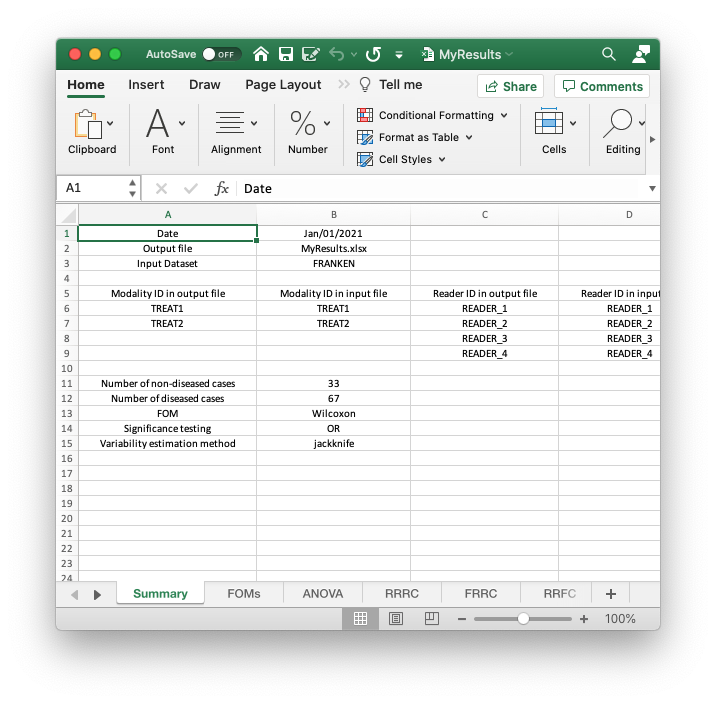
\includegraphics[width=0.5\linewidth,height=0.2\textheight]{R/quick-start/MyResultsSummary} 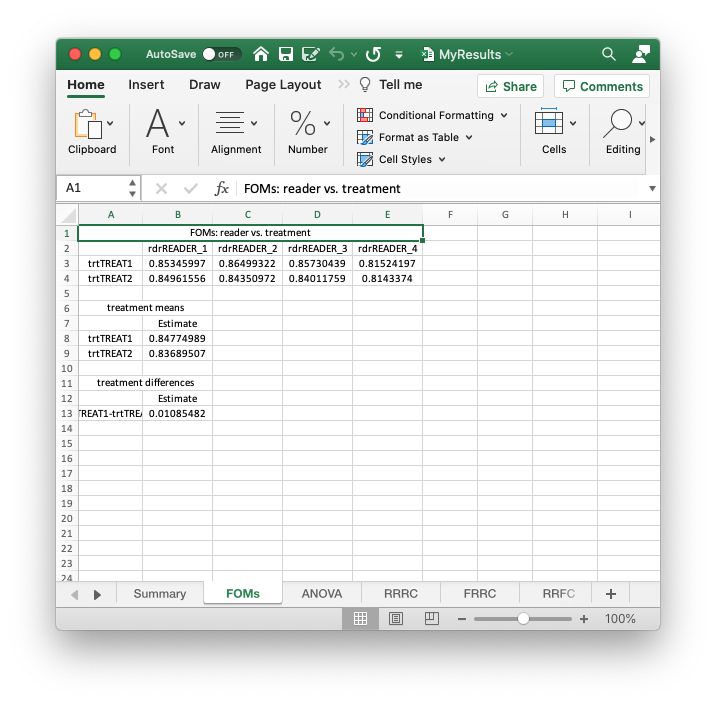
\includegraphics[width=0.5\linewidth,height=0.2\textheight]{R/quick-start/MyResultsFOMs} 

}

\caption{`Summary` and `FOMs` worksheets of Excel file `R/quick-start/MyResults.xlsx`}\label{fig:quick-start-or-xlsx1}
\end{figure}

\begin{figure}

{\centering 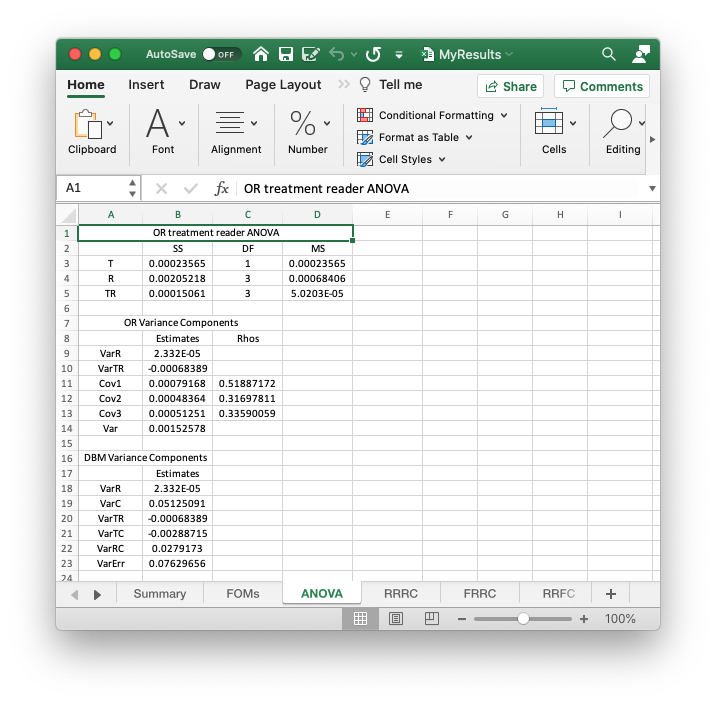
\includegraphics[width=0.5\linewidth,height=0.2\textheight]{R/quick-start/MyResultsANOVA1} 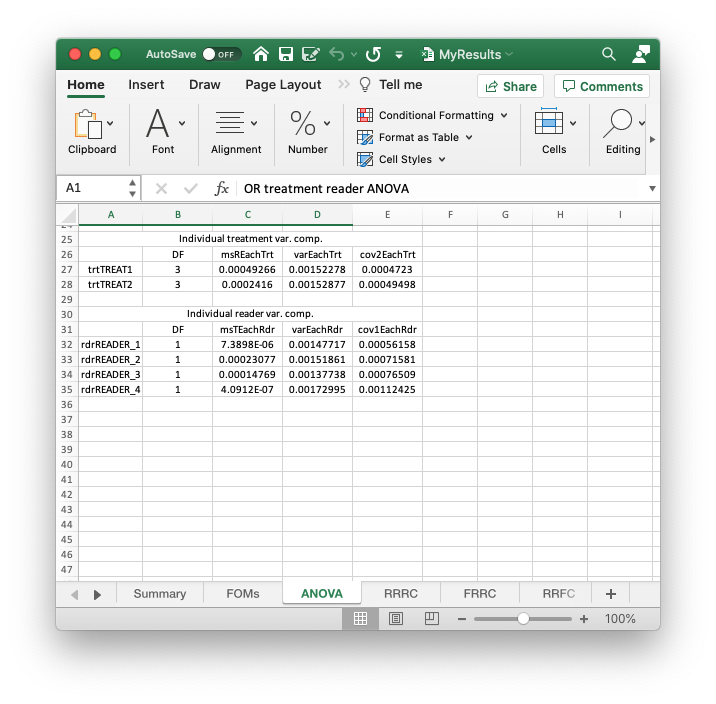
\includegraphics[width=0.5\linewidth,height=0.2\textheight]{R/quick-start/MyResultsANOVA2} 

}

\caption{`ANOVA` worksheet of Excel file `R/quick-start/MyResults.xlsx`}\label{fig:quick-start-or-xlsx2}
\end{figure}

\begin{figure}

{\centering 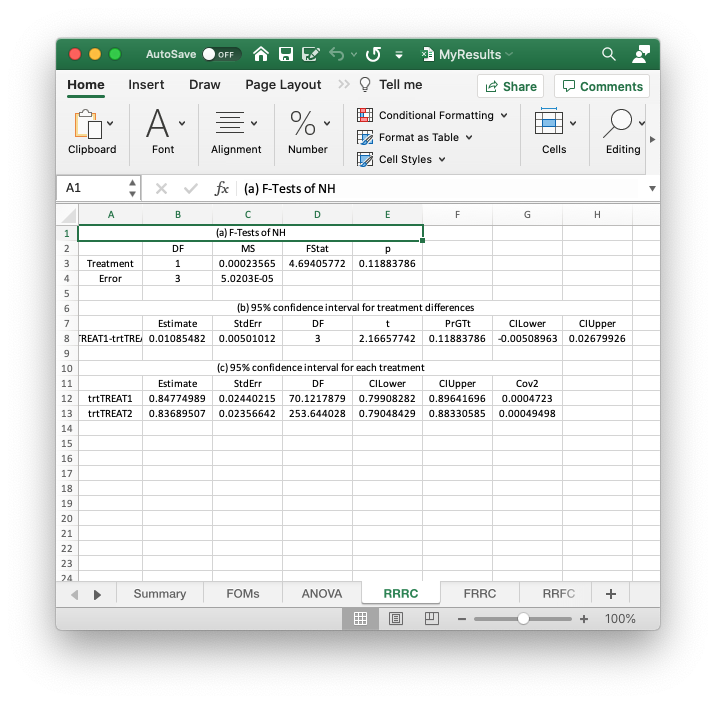
\includegraphics[width=0.5\linewidth,height=0.2\textheight]{R/quick-start/MyResultsRRRC} 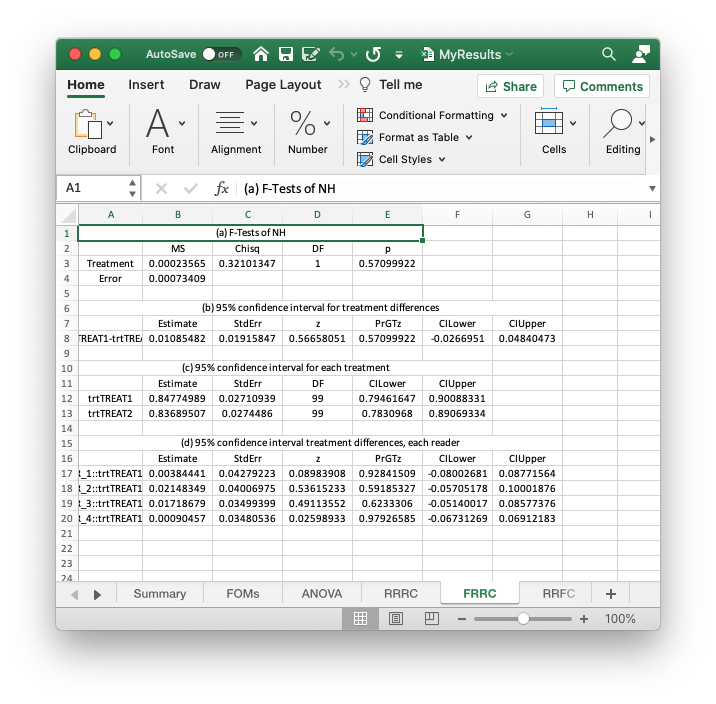
\includegraphics[width=0.5\linewidth,height=0.2\textheight]{R/quick-start/MyResultsFRRC} 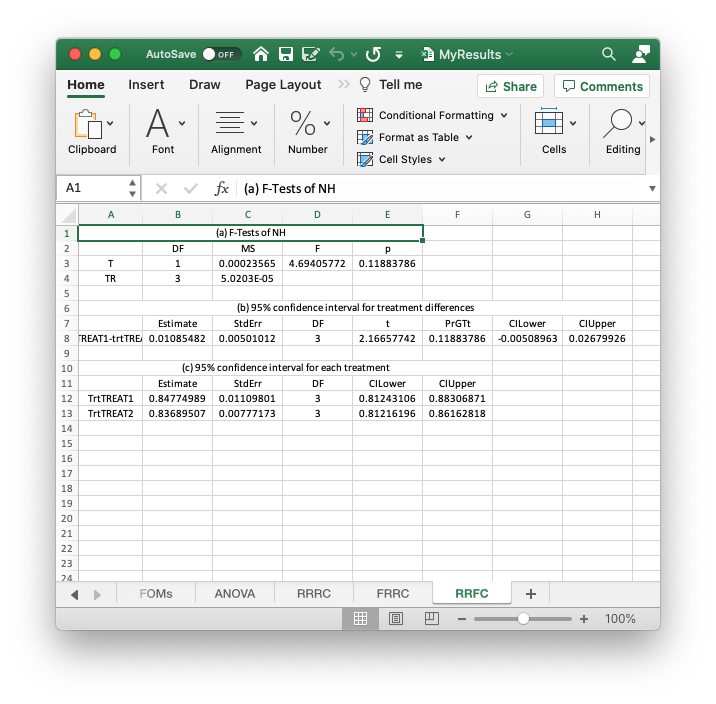
\includegraphics[width=0.5\linewidth,height=0.2\textheight]{R/quick-start/MyResultsRRFC} 

}

\caption{`RRRC`, `FRRC` and `RRFC` worksheets of Excel file `R/quick-start/MyResults.xlsx`}\label{fig:quick-start-or-xlsx3}
\end{figure}

\hypertarget{quick-start-or-excel-references}{%
\section{References}\label{quick-start-or-excel-references}}

\hypertarget{dbm-analysis-background}{%
\chapter{DBM method background}\label{dbm-analysis-background}}

\hypertarget{dbm-analysis-background-how-much-finished}{%
\section{TBA How much finished}\label{dbm-analysis-background-how-much-finished}}

80\%

\hypertarget{dbm-analysis-background-introduction}{%
\section{Introduction}\label{dbm-analysis-background-introduction}}

The term \emph{treatment} is generic for \emph{imaging system}, \emph{modality} or \emph{image processing}; \emph{reader} is generic for \emph{radiologist} or \emph{algorithmic observer}, e.g., a computer aided detection (CAD) or artificial intelligence (AI) algorithm. The previous chapter described analysis of a single ROC dataset and comparing the observed area \(AUC\) under the ROC plot to a specified value. Clinically this is not an interesting problem; rather, interest is usually in comparing performance of a group of readers interpreting a common set of cases in two or more treatments. Such data is termed multiple reader multiple case (MRMC). {[}An argument could be made in favor of the term ``multiple-treatment multiple-reader'', since ``multiple-case'' is implicit in any ROC analysis that takes into account correct and incorrect decisions on cases. However, I will stick with existing terminology.{]} The basic idea is that by sampling a sufficiently large number of readers and cases one can draw conclusions that apply broadly to other readers of similar skill levels interpreting other similar case sets in the selected treatments. How one accomplishes this, termed MRMC analysis, is the subject of this chapter.

This chapter describes the first truly successful method of analyzing MRMC ROC data, namely the Dorfman-Berbaum-Metz (DBM) method \citep{RN204}. The other method, due to Obuchowski and Rockette \citep{RN1450}, is the subject of Chapter 10 (TBA). Both methods have been substantially improved by Hillis \citep{RN1866, RN1865, RN2508}. It is not an overstatement that ROC analysis came of age with the methods described in this chapter. Prior to the techniques described here, one knew of the existence of sources of variability affecting a measured \(AUC\) value, as discussed in (book) Chapter 07, but then-known techniques \citep{RN412} for estimating the corresponding variances and correlations were impractical.

\hypertarget{historical-background}{%
\subsection{Historical background}\label{historical-background}}

The author was thrown (unprepared) into the methodology field ca. 1985 when, as a junior faculty member, he undertook comparing a prototype digital chest-imaging device (Picker International, ca. 1983) vs.~an optimized analog chest-imaging device at the University of Alabama at Birmingham. At the outset a decision was made to use free-response ROC methodology instead of ROC, as the former accounted for lesion localization, and I and my mentor, Prof.~Gary T. Barnes, were influenced in that decision by a publication \citep{bunch1977free} to be described in (book) Chapter 12. Therefore, instead of ROC-AUC one had lesion-level sensitivity at a fixed number of location level false positives per case as the figure-of-merit (FOM). Details of the FOM are not relevant at this time. Suffice to state that methods described in this chapter, which had not been developed in 1983, while developed for analyzing reader-averaged inter-treatment ROC-AUC differences, \emph{apply to any scalar FOM}. While I was successful at calculating confidence intervals (this is the heart of what is loosely termed \emph{statistical analysis}) and publishing the work \citep{Chakraborty1986DigitalVsConv} using techniques described in a book \citep{RN412} titled ``Evaluation of Diagnostic Systems: Methods from Signal Detection Theory'', subsequent attempts at applying these methods in a follow-up paper \citep{Niklason1986SimulatedPulmonary} led to negative variance estimates (private communication, Dr.~Loren Niklason, ca. 1985). With the benefit of hindsight, negative variance estimates are not that uncommon and the method to be described in this chapter has to deal with that possibility.

The methods \citep{RN412} described in the cited book involved estimating the different variability components -- case sampling, between-reader and within-reader variability. Between-reader and within-reader variability (the two cannot be separated as discussed in (book) Chapter 07) could be estimated from the variance of the \(AUC\) values corresponding to the readers interpreting the cases within a treatment and then averaging the variances over all treatments. Estimating case-sampling and within-reader variability required splitting the dataset into a few smaller subsets (e.g., a case set with 60 cases might be split into 3 sub-sets of 20 cases each), analyzing each subset to get an \(AUC\) estimate, calculating the variance of the resulting \(AUC\) values \citep{RN412} and scaling the result to the original case size. Because it was based on few values, the estimate was inaccurate, and the already case-starved original dataset made it difficult to estimate AUCs for the subsets; moreover, the division into subsets was at the discretion of the researcher, and therefore unlikely to be reproduced by others. Estimating within-reader variability required re-reading the entire case set, or at least a part of it. ROC studies have earned a deserved reputation for taking much time to complete, and having to re-read a case set was not a viable option. {[}Historical note: I recalls a barroom conversation with Dr.~Thomas Mertelmeir after the conclusion of an SPIE meeting ca. 2004, where Dr.~Mertelmeir commiserated mightily, over several beers, about the impracticality of some of the ROC studies required of imaging device manufacturers by the FDA.{]}

\hypertarget{the-wagner-analogy}{%
\subsection{The Wagner analogy}\label{the-wagner-analogy}}

An important objective of modality comparison studies is to estimate the variance of the difference in reader-averaged AUCs between the treatments. For two treatments one sums the reader-averaged variance in each treatment and subtracts twice the covariance (a scaled version of the correlation). Therefore, in addition to estimating variances, one needs to estimate correlations. Correlations are present due to the common case set interpreted by the readers in the different treatments. If the correlation is large, i.e., close to unity, then the individual treatment variances tend to cancel, making the constant treatment-induced difference easier to detect. The author recalls a vivid analogy used by the late Dr.~Robert F. Wagner to illustrate this point at an SPIE meeting ca. 2008. To paraphrase him, \emph{consider measuring from shore the heights of the masts on two adjacent boats in a turbulent ocean. Because of the waves, the heights, as measured from shore, are fluctuating wildly, so the variance of the individual height measurements is large. However, the difference between the two heights is likely to be relatively constant, i.e., have small variance. This is because the wave that causes one mast's height to increase also increases the height of the other mast.}

\hypertarget{the-shortage-of-numbers-to-analyze-and-a-pivotal-breakthrough}{%
\subsection{The shortage of numbers to analyze and a pivotal breakthrough}\label{the-shortage-of-numbers-to-analyze-and-a-pivotal-breakthrough}}

\emph{The basic issue was that the calculation of \(AUC\) reduces the relatively large number of ratings of a set of non-diseased and diseased cases to a single number.} For example, after completion of an ROC study with 5 readers and 100 non-diseased and 100 diseased cases interpreted in two treatments, the data is reduced to just 10 numbers, i.e., five readers times two treatments. It is difficult to perform statistics with so few numbers. The author recalls a conversation with Prof.~Kevin Berbaum at a Medical Image Perception Society meeting in Tucson, Arizona, ca. 1997, in which he described the basic idea that forms the subject of this chapter. Namely, using jackknife pseudovalues (to be defined below) as individual case-level figures of merit. This, of course, greatly increases the amount of data that one can work with; instead of just 10 numbers one now has 2,000 pseudovalues (2 x 5 x 200). If one assumes the pseudovalues behave essentially as case-level data, then by assumption they are independent and identically distributed, and therefore satisfy the conditions for application of standard analysis of variance (ANOVA) techniques. {[}This assumption has been much criticized and is the basis for some preferring alternate approaches - but, as Hillis has stated, and I paraphrase, the pseudovalue based method ``works'', but lacks sufficient rigor.{]} The relevant paper had already been published in 1992 but other projects and lack of formal statistical training kept me from fully appreciating this work until later.

For the moment I restrict to fully paired data (i.e., each case is interpreted by all readers in all treatments). There is a long history of how this field has evolved and I cannot do justice to all methods that are currently available. Some of the methods \citep{RN1441, RN2013, RN1451} have the advantage that they can handle explanatory variables (termed covariates) that could influence performance, e.g., years of experience, types of cases, etc. Other methods are restricted to specific choices of FOM. Specifically, the probabilistic approach \citep{RN2253, RN2254, RN2351, RN2080} is restricted to the empirical \(AUC\) under the ROC curve, and is not applicable to other FOMs, e.g., parametrically fitted ROC AUCs or, more importantly, to location specific paradigm FOMs. Instead, I will focus on methods for which software is readily available (i.e., freely on websites), which have been widely used (the method that I am about to describe has been used in several hundred publications) and validated via simulations, and which apply to any scalar figure of merit, and therefore widely applicable, for example, to location specific paradigms.

\hypertarget{organization-of-chapter}{%
\subsection{Organization of chapter}\label{organization-of-chapter}}

The concepts of reader and case populations, introduced in (book) Chapter 07, are recapitulated. A distinction is made between \emph{fixed} and \emph{random} factors -- statistical terms with which one must become familiar. Described next are three types of analysis that are possible with MRMC data, depending on which factors are regarded as random and which as fixed. The general approach to the analysis is described. Two methods of analysis are possible: the jackknife pseudovalue-based approach detailed in this chapter and an alternative approach is detailed in Chapter 10. The Dorfman-Berbaum-Metz (DBM) model for the jackknife pseudovalues is described that incorporates different sources of variability and correlations possible with MRMC data. Calculation of ANOVA-related quantities, termed mean squares, from the pseudovalues, are described followed by the significance testing procedure for testing the null hypothesis of no treatment effect. A relevant distribution used in the analysis, namely the F-distribution, is illustrated with R examples. The decision rule, i.e., whether to reject the NH, calculation of the ubiquitous p-value, confidence intervals and how to handle multiple treatments is illustrated with two datasets, one an older ROC dataset that has been widely used to demonstrate advances in ROC analysis, and the other a recent dataset involving evaluation of digital chest tomosynthesis vs.~conventional chest imaging. The approach to validation of DBM analysis is illustrated with an R example. The chapter concludes with a section on the meaning of the pseudovalues. The intent is to explain, at an intuitive level, why the DBM method ``works'', even though use of pseudovalues has been questioned at the conceptual level. For organizational reasons and space limitations, details of the software are relegated to Online Appendices, but they are essential reading, preferably in front of a computer running the online software that is part of this book. The author has included material here that may be obvious to statisticians, e.g., an explanation of the Satterthwaite approximation, but are expected to be helpful to others from non-statistical backgrounds.

\hypertarget{dbm-analysis-background-random-fixed-factors}{%
\section{Random and fixed factors}\label{dbm-analysis-background-random-fixed-factors}}

\emph{This paragraph introduces some analysis of variance (ANOVA) terminology. Treatment, reader and case are factors with different numbers of levels corresponding to each factor. For an ROC study with two treatments, five readers and 200 cases, there are two levels of the treatment factor, five levels of the reader factor and 200 levels of the case factor. If a factor is regarded as fixed, then the conclusions of the analysis apply only to the specific levels of the factor used in the study. If a factor is regarded as random, the levels of the factor are regarded as random samples from a parent population of the corresponding factor, and conclusions regarding specific levels are not allowed; rather, conclusions apply to the distribution from which the levels were sampled.}

ROC MRMC studies require a sample of cases and interpretations by one or more readers in one or more treatments (in this book the term \emph{multiple} includes as a special case \emph{one}). A study is never conducted on a sample of treatments. It would be nonsensical to image patients using a ``sample'' of all possible treatments. Every variation of an imaging technique (e.g., different kilovoltage or kVp) or display method (e.g., window-level setting) or image processing techniques qualifies as a distinct treatment. The number of possible treatments is very large, and, from a practical point of view, most of them are uninteresting. Rather, interest is in comparing two or more (a few at most) treatments that, based on preliminary studies, are clinically interesting. One treatment may be computed tomography, the other magnetic resonance imaging, or one may be interested in comparing a standard image processing method to a newly proposed one, or one may be interested in comparing CAD to a group of readers.

This brings out an essential difference between how cases, readers and treatments have to be regarded in the variability estimation procedure. Cases and readers are usually regarded as random factors (there has to be at least one random factor -- if not, there are no sources of variability and nothing to apply statistics to!), while treatments are regarded as fixed factors. The random factors contribute variability, but the fixed factors do not, rather they contribute constant shifts in performance. The terms \emph{fixed} and \emph{random} factors are used in this specific sense, and are derived, in turn, from ANOVA methods in statistics. With two or more treatments, there are shifts in performance of treatments relative to each other, that one seeks to assess the significance of, against a background of noise contributed by the random factors. If the shifts are sufficiently large compared to the noise, then one can state, with some certainty, that they are real. Quantifying the last statement uses the methods of hypothesis testing described in book chapter TBA introduced in Chapter (hypothesis-testing).

\hypertarget{dbm-analysis-background-reader-case-populations}{%
\section{Reader and case populations}\label{dbm-analysis-background-reader-case-populations}}

Consider a sample of \(J\) readers. Conceptually there is a reader-population, modeled as a normal distribution \(\theta_j \sim N\left ( \theta_{\bullet\{1\}}, \sigma_{br+wr}^{2} \right )\), describing the variation of skill-level of readers. Here \(\theta\) is a generic FOM. Each reader \(j\) is characterized by a different value of \(\theta_j\), \(j=1,2,...J\) and one can conceptually think of a bell-shaped curve with variance \(\sigma_{br+wr}^{2}\) describing between-reader variability of the readers. A large variance implies large spread in reader skill levels.

Likewise, there is a case-population, also modeled as a normal distribution, describing the variations in difficulty levels of the patients. One actually has two unit-variance distributions, one for non-diseased and one for diseased cases, characterized by a separation parameter. The separation parameter is scaled (i.e., normalized) by the standard deviation of each distribution (assumed equal). Each distribution has unit variance. Conceptually an easy case set has a larger than usual scaled separation parameter while a difficult case set has a smaller than usual scaled separation parameter. The distribution of the scaled separation parameter can be modeled as a bell-shaped curve \(\theta_{\{c\}} \sim N\left ( \theta_{\{\bullet\}}, \sigma_{cs+wr}^{2} \right )\) with variance \(\sigma_{cs+wr}^{2}\) describing the variations in difficulty levels of different case samples. Note the need for the case-set index, introduced in (book) Chapter 07, to specify the separation parameter for a specific case-set (in principle a \(j\)-index is also needed as one cannot have an interpretation without a reader; for now it is suppressed. A small variance \(\sigma_{cs}^{2}\) implies the different case sets have similar difficulty levels while a larger variance would imply a larger spread in difficulty levels. Just as the previous paragraph described reader-varibility, this paragraph has described case-variability.

\emph{Anytime one has a common random component to two measurements, the measurements are correlated.} In the Wagner analogy, the common component is the random height, as a function of time, of a wave, which contributes the same amount to both height measurements (since the boats are adjacent). Since the readers interpret a common case set in all treatments one needs to account for various types of correlations that are potentially present. These occur due to the various types of pairings that can occur with MRMC data, where each pairing implies the presence of a common component to the measurements: (a) the same reader interpreting the \emph{same cases} in different treatments, (b) different readers interpreting the \emph{same cases} in the same treatment and (c) different readers interpreting the \emph{same cases} in different treatments. These pairings are more clearly elucidated in (book) Chapter 10. The current chapter uses jackknife pseudovalue based analysis to model the variances and the correlations. Hillis has shown that the two approaches are essentially equivalent \citep{RN1866}.

\hypertarget{dbm-analysis-background-threeAnalyses}{%
\section{Three types of analyses}\label{dbm-analysis-background-threeAnalyses}}

\emph{MRMC analysis aims to draw conclusions regarding the significances of inter-treatment shifts in performance. Ideally a conclusion (i.e., a difference is significant) should generalize to the respective populations from which the random samples were obtained. In other words, the idea is to generalize from the observed samples to the underlying populations. Three types of analyses are possible depending on which factor(s) one regards as random and which as fixed: random-reader random-case (RRRC), fixed-reader random-case (FRRC) and random-reader fixed-case (RRFC). If a factor is regarded as random, then the conclusion of the study applies to the population from which the levels of the factor were sampled. If a factor is regarded as fixed, then the conclusion applies only to the specific levels of the sampled factor. For example, if reader is regarded as a random factor, the conclusion generalizes to the reader population from which the readers used in the study were obtained. If reader is regarded as a fixed factor, then the conclusion applies to the specific readers that participated in the study. Regarding a factor as fixed effectively ``freezes out'' the sampling variability of the population and interest then centers only on the specific levels of the factor used in the study. Likewise, treating case as a fixed factor means the conclusion of the study is specific to the case-set used in the study.}

\hypertarget{dbm-analysis-background-approach}{%
\section{General approach}\label{dbm-analysis-background-approach}}

This section provides an overview of the steps involved in analysis of MRMC data. Two approaches are described in parallel: a figure of merit (FOM) derived jackknife pseudovalue based approach, detailed in this chapter and an FOM based approach, detailed in the next chapter. The analysis proceeds as follows:

\begin{enumerate}
\def\labelenumi{\arabic{enumi}.}
\tightlist
\item
  A FOM is selected: \emph{the selection of FOM is the single-most critical aspect of analyzing an observer performance study}. The selected FOM is denoted \(\theta\). The FOM has to be an objective scalar measure of performance with larger values characterizing better performance. {[}The qualifier ``larger'' is trivially satisfied; if the figure of merit has the opposite characteristic, a sign change is all that is needed to bring it back to compliance with this requirement.{]} Examples are empirical \(AUC\), the binormal model-based estimate \(A_z\) , other advance method based estimates of \(AUC\), sensitivity at a predefined value of specificity, etc. An example of a FOM requiring a sign-change is \(FPF\) at a specified \(TPF\), where smaller values signify better performance.
\item
  For each treatment \(i\) and reader \(j\) the figure of merit \(\theta_{ij}\) is estimated from the ratings data. Repeating this over all treatments and readers yields a matrix of observed values \(\theta_{ij}\). This is averaged over all readers in each treatment yielding \(\theta_{i\bullet}\). The observed effect-size \(ES_{obs}\) is defined as the difference between the reader-averaged FOMs in the two treatments, i.e., \(ES_{obs} = \theta_{2\bullet}-\theta_{1\bullet}\). While extensible to more than two treatments, the explanation is more transparent by restricting to two modalities.
\item
  If the magnitude of \(ES_{obs}\) is ``large'' one has reason to suspect that there might indeed be a significant difference in AUCs between the two treatments, where \emph{significant} is used in the sense of (book) Chapter 08. Quantification of this statement, specifically how large is ``large'', requires the conceptually more complex steps described next.

  \begin{itemize}
  \tightlist
  \item
    In the DBM approach, the subject of this chapter, jackknife pseudovalues are calculated as described in Chapter 08. A standard ANOVA model with uncorrelated errors is used to model the pseudovalues.
  \item
    In the OR approach, the subject of the next chapter, the FOM is modeled directly using a custom ANOVA model with correlated errors.
  \end{itemize}
\item
  Depending on the selected method of modeling the data (pseudovalue vs.~FOM) a statistical model is used which includes parameters modeling the true values in each treatment, and expected variations due to different variability components in the model, e.g., between-reader variability, case-sampling variability, interactions (e.g., allowing for the possibility that the random effect of a given reader could be treatment dependent) and the presence of correlations (between pseudovalues or FOMs) because of the pairings inherent in the interpretations.
\item
  In RRRC analysis one accounts for randomness in readers and cases. In FRRC analysis one regards reader as a fixed factor. In RRFC analysis one regards the case-sample (set of cases) as a fixed factor. The statistical model depends on the type of analysis.
\item
  The parameters of the statistical model are estimated from the observed data.
\item
  The estimates are used to infer the statistical distribution of the observed effect size, \(ES_{obs}\), regarded as a realization of a random variable, under the null hypothesis (NH) that the true effect size is zero.
\item
  Based on this statistical distribution, and assuming a two-sided test, the probability (this is the oft-quoted p-value) of obtaining an effect size at least as extreme as that actually observed, is calculated, as in (book) Chapter 08.
\item
  If the p-value is smaller than a preselected value, denoted \(\alpha\), one declares the treatments different at the \(\alpha\) - significance level. The quantity \(\alpha\) is the control (or ``cap'') on the probability of making a Type I error, defined as rejecting the NH when it is true. It is common to set \(\alpha\) = 0.05 but depending on the severity of the consequences of a Type I error, as discussed in (book) Chapter 08, one might consider choosing a different value. Notice that \(\alpha\) is a pre-selected number while the p-value is a realization (observation) of a random variable.
\item
  For a valid statistical analysis, the empirical probability \(\alpha_{emp}\) over many (typically 2000) independent NH datasets, that the p-value is smaller than \(\alpha\), should equal \(\alpha\) to within statistical uncertainty.
\end{enumerate}

\hypertarget{dbm-analysis-background-summary}{%
\section{Summary TBA}\label{dbm-analysis-background-summary}}

This chapter has detailed analysis of MRMC ROC data using the DBM method. A reason for the level of detail is that almost all of the material carries over to other data collection paradigms, and a thorough understanding of the relatively simple ROC paradigm data is helpful to understanding the more complex ones.

DBM has been used in several hundred ROC studies (Prof.~Kevin Berbaum, private communication ca. 2010). While the method allows generalization of a study finding, e.g., rejection of the NH, to the population of readers and cases, I believe this is sometimes taken too literally. If a study is done at a single hospital, then the radiologists tend to be more homogenous as compared to sampling radiologists from different hospitals. This is because close interactions between radiologists at a hospital tend to homogenize reading styles and performance. A similar issue applies to patient characteristics, which are also expected to vary more between different geographical locations than within a given location served by the hospital. This means is that single hospital study based p-values may tend to be biased downwards, declaring differences that may not be replicable if a wider sampling ``net'' were used using the same sample size. The price paid for a wider sampling net is that one must use more readers and cases to achieve the same sensitivity to genuine treatment effects, i.e., statistical power (i.e., there is no ``free-lunch'').

A third MRMC ROC method, due to Clarkson, Kupinski and Barrett19,20, implemented in open-source JAVA software by Gallas and colleagues22,44 (\url{http://didsr.github.io/iMRMC/}) is available on the web. Clarkson et al19,20 provide a probabilistic rationale for the DBM model, provided the figure of merit is the empirical \(AUC\). The method is elegant but it is only applicable as long as one is using the empirical AUC as the figure of merit (FOM) for quantifying observer performance. In contrast the DBM approach outlined in this chapter, and the approach outlined in the following chapter, are applicable to any scalar FOM. Broader applicability ensures that significance-testing methods described in this, and the following chapter, apply to other ROC FOMs, such as binormal model or other fitted AUCs, and more importantly, to other observer performance paradigms, such as free-response ROC paradigm. An advantage of the Clarkson et al.~approach is that it predicts truth-state dependence of the variance components. One knows from modeling ROC data that diseased cases tend to have greater variance than non-diseased ones, and there is no reason to suspect that similar differences do not exist between the variance components.

Testing validity of an analysis method via simulation testing is only as good as the simulator used to generate the datasets, and this is where current research is at a bottleneck. The simulator plays a central role in ROC analysis. In my opinion this is not widely appreciated. In contrast, simulators are taken very seriously in other disciplines, such as cosmology, high-energy physics and weather forecasting. The simulator used to validate3 DBM is that proposed by Roe and Metz39 in 1997. This simulator has several shortcomings. (a) It assumes that the ratings are distributed like an equal-variance binormal model, which is not true for most clinical datasets (recall that the b-parameter of the binormal model is usually less than one). Work extending this simulator to unequal variance has been published3. (b) It does not take into account that some lesions are not visible, which is the basis of the contaminated binormal model (CBM). A CBM model based simulator would use equal variance distributions with the difference that the distribution for diseased cases would be a mixture distribution with two peaks. The radiological search model (RSM) of free-response data, Chapter 16 \&17 also implies a mixture distribution for diseased cases, and it goes farther, as it predicts some cases yield no z-samples, which means they will always be rated in the lowest bin no matter how low the reporting threshold. Both CBM and RSM account for truth dependence by accounting for the underlying perceptual process. (c) The Roe-Metz simulator is out dated; the parameter values are based on datasets then available (prior to 1997). Medical imaging technology has changed substantially in the intervening decades. (d) Finally, the methodology used to arrive at the proposed parameter values is not clearly described. Needed is a more realistic simulator, incorporating knowledge from alternative ROC models and paradigms that is calibrated, by a clearly defined method, to current datasets.

Since ROC studies in medical imaging have serious health-care related consequences, no method should be used unless it has been thoroughly validated. Much work still remains to be done in proper simulator design, on which validation is dependent.

\hypertarget{dbm-analysis-background-references}{%
\section{References}\label{dbm-analysis-background-references}}

\hypertarget{dbm-analysis-significance-testing}{%
\chapter{Significance Testing using the DBM Method}\label{dbm-analysis-significance-testing}}

\hypertarget{dbm-analysis-significance-testing-how-much-finished}{%
\section{TBA How much finished}\label{dbm-analysis-significance-testing-how-much-finished}}

60\%

\hypertarget{the-dbm-sampling-model}{%
\section{The DBM sampling model}\label{the-dbm-sampling-model}}

DBM = Dorfman Berbaum Metz

The figure-of-merit has three indices:

\begin{itemize}
\tightlist
\item
  A treatment index \(i\), where \(i\) runs from 1 to \(I\), where \(I\) is the total number of treatments.\\
\item
  A reader index \(j\), where \(j\) runs from 1 to \(J\), where \(J\) is the total number of readers.\\
\item
  The case-sample index \(\{c\}\), where \(\{1\}\) i.e., \(c\) = 1, denotes a set of cases, \(K_1\) non-diseased and \(K_2\) diseased, interpreted by all readers in all treatments, and other integer values of \(c\) correspond to other independent sets of cases that, although not in fact interpreted by the readers, could potentially be ``interpreted'' using resampling methods such as the bootstrap or the jackknife.
\end{itemize}

The approach \citep{RN204} taken by DBM was to use the jackknife resampling method to calculate FOM pseudovalues \({Y'}_{ijk}\) defined by (the reason for the prime will become clear shortly):

\begin{equation}
Y'_{ijk}=K\theta_{ij}-(K-1)\theta_{ij(k)}
\label{eq:pseudoValPrime}
\end{equation}

Here \(\theta_{ij}\) is the estimate of the figure-of-merit for reader \(j\) interpreting all cases in treatment \(i\) and \(\theta_{ij(k)}\) is the corresponding figure of merit with case \(k\) \emph{deleted} from the analysis. To keep the notation compact the case-sample index \(\{1\}\) on every figure of merit symbol is suppressed.

Recall from book Chapter 07 that the jackknife is a way of teasing out the case-dependence: the left hand side of Equation \eqref{eq:pseudoValPrime} has a case index \(k\), with \(k\) running from 1 to \(K\), where \(K\) is the total number of cases: \(K=K_1+K_2\).

Hillis et al \citep{RN1866} proposed a centering transformation on the pseudovalues (he terms it ``normalized'' pseudovalues, but to me ``centering'' is a more accurate and descriptive term - \emph{Normalize: (In mathematics) multiply (a series, function, or item of data) by a factor that makes the norm or some associated quantity such as an integral equal to a desired value (usually 1). New Oxford American Dictionary, 2016}):

\begin{equation}
Y_{ijk}=Y'_{ijk}+\left (\theta_{ij} - Y'_{ij\bullet}  \right )
\label{eq:pValCentered}
\end{equation}

\textbf{Note: the bullet symbol denotes an average over the corresponding index.}

The effect of this transformation is that the average of the centered pseudovalues over the case index is identical to the corresponding estimate of the figure of merit:

\begin{equation}
Y_{ij\bullet}=Y'_{ij\bullet}+\left (\theta_{ij} - Y'_{ij\bullet}  \right )=\theta_{ij}
\label{eq:EffectOfCentering}
\end{equation}

This has the advantage that all confidence intervals are properly centered. The transformation is unnecessary if one uses the Wilcoxon as the figure-of-merit, as the pseudovalues calculated using the Wilcoxon as the figure of merit are ``naturally'' centered, i.e.,

\(\theta_{ij} - Y'_{ij\bullet} = 0\)

\emph{It is understood that, unless explicitly stated otherwise, all calculations from now on will use centered pseudovalues.}

Consider \(N\) replications of a MRMC study, where a replication means repetition of the study with the same treatments, readers and case-set \(\{C=1\}\). For \(N\) replications per treatment-reader-case combination, the DBM model for the pseudovalues is (\(n\) is the replication index, usually \(n\) = 1, but kept here for now):

\begin{equation}
Y_{n(ijk)}  = \mu + \tau_i+ R_j + C_k + (\tau R)_{ij}+ (\tau C)_{ik}+ (R C)_{jk} + (\tau RC)_{ijk}+ \epsilon_{n(ijk)} 
\label{eq:DefDBMModel}
\end{equation}

The term \(\mu\) is a constant. By definition, the treatment effect \(\tau_i\) is subject to the constraint:

\begin{equation}
\sum_{i=1}^{I}\tau_i=0\Rightarrow \tau_\bullet=0
\label{eq:constraintTau}
\end{equation}

This constraint ensures that \(\mu\) has the interpretation of the average of the pseudovalues over treatments, readers and cases.

The (nesting) notation for the replication index, i.e., \(n(ijk)\), implies \(n\) observations for treatment-reader-case combination \(ijk\). With no replications (\(N\) = 1) it is convenient to omit the n-symbol.

The parameter \(\tau_i\) is estimated as follows:

\begin{equation}
Y_{ijk} \equiv Y_{1(ijk)}\\
\tau_i = Y_{i \bullet \bullet} -Y_{\bullet \bullet \bullet} 
\label{eq:estimatingTau}
\end{equation}

\emph{The basic assumption of the DBM model is that the pseudovalues can be regarded as independent and identically distributed observations. That being the case, the pseudovalues can be analyzed by standard ANOVA techniques.} Since pseduovalues are computed from a common dataset, this assumption is, non-intuitive. However, for the special case of Wilcoxon figure of merit, it is justified.

\hypertarget{explanation-of-terms-in-the-model}{%
\subsection{Explanation of terms in the model}\label{explanation-of-terms-in-the-model}}

The right hand side of Eqn. \eqref{eq:pseudoValPrime} consists of one fixed and 7 random effects. The current analysis assumes readers and cases as random factors (RRRC), so by definition \(R_j\) and \(C_k\) are random effects, and moreover, any term that includes a random factor is a random effect; for example, \((\tau R)_{ij}\) is a random effect because it includes the \(R\) factor. Here is a list of the random terms:

\begin{equation}
R_j, C_k, (\tau R)_{ij}, (\tau C)_{ik}, (RC)_{jk},  (\tau RC)_{ijk},  \epsilon_{ijk}
\label{eq:DBMRandomTerms}
\end{equation}

\textbf{Assumption:} Each of the random effects is modeled as a random sample from mutually independent zero-mean normal distributions with variances as specified below:

\begin{align}
\left.\begin{array}{rll}
{R_j}&\sim& N\left ( 0,\sigma_{R}^{2} \right ) \\[0.5em]
{C_k}&\sim& N\left ( 0,\sigma_{C}^{2} \right ) \\[0.5em]
{(\tau R)_{ij}}&\sim& N\left ( 0,\sigma_{\tau R}^{2} \right ) \\[0.5em]
{(\tau C)_{ik}}&\sim& N\left ( 0,\sigma_{\tau C}^{2} \right ) \\[0.5em]
{(RC)_{jk}}&\sim& N\left ( 0,\sigma_{RC}^{2} \right ) \\[0.5em]
{(\tau RC)_{ijk}}&\sim& N\left ( 0,\sigma_{\tau RC}^{2} \right ) \\[0.5em]
\epsilon_{ijk} &\sim& N\left ( 0,\sigma_{\epsilon}^{2} \right )
\end{array}\right\}
\label{eq:samplingOfDbmTerms}
\end{align}

Equation \eqref{eq:samplingOfDbmTerms} defines the meanings of the variance components appearing in Equation \eqref{eq:DBMRandomTerms}. One could have placed a \(Y\) subscript (or superscript) on each of the variances, as they describe fluctuations of the pseudovalues, not FOM values. However, this tends to clutter the notation. So here is the convention:

\textbf{Unless explicitly stated otherwise, all variance symbols in this chapter refer to pseudovalues. }
Another convention: \((\tau R)_{ij}\) is \emph{not} the product of the treatment and reader factors, rather it is a single factor, namely the treatment-reader factor with \(IJ\) levels, subscripted by the index \(ij\) and similarly for the other product-like terms in Equation \eqref{eq:samplingOfDbmTerms}.

\hypertarget{meanings-of-variance-components-in-the-dbm-model-tba-this-section-can-be-improved}{%
\subsection{\texorpdfstring{Meanings of variance components in the DBM model (\textbf{TBA this section can be improved})}{Meanings of variance components in the DBM model (TBA this section can be improved)}}\label{meanings-of-variance-components-in-the-dbm-model-tba-this-section-can-be-improved}}

The variances defined in \eqref{eq:samplingOfDbmTerms} are collectively termed \emph{variance components}. Specifically, they are jackknife pseudovalue variance components, to be distinguished from figure of merit (FOM) variance components to be introduced in TBA Chapter 10. They are in order: \(\sigma_{R}^{2} ,\sigma_{C}^{2} \sigma_{\tau R}^{2},\sigma_{\tau C}^{2},\sigma_{RC}^{2}, \sigma_{\tau RC}^{2},\sigma_{\epsilon}^{2}\). They have the following meanings.

\begin{itemize}
\tightlist
\item
  The term \(\sigma_{R}^{2}\) is the variance of readers that is independent of treatment or case, which are modeled separately. It is not to be confused with the terms \(\sigma_{br+wr}^{2}\) and \(\sigma_{cs+wr}^{2}\) used in §9.3, which describe the variability of \(\theta\) measured under specified conditions. {[}A jackknife pseudovalue is a weighted difference of FOM like quantities, TBA \eqref{eq:pseudoValPrime}. Its meaning will be explored later. For now, \emph{a pseudovalue variance is distinct from a FOM variance}.{]}
\item
  The term \(\sigma_{C}^{2}\) is the variance of cases that is independent of treatment or reader.
\item
  The term \(\sigma_{\tau R}^{2}\) is the treatment-dependent variance of readers that was excluded in the definition of \(\sigma_{R}^{2}\). If one were to sample readers and treatments for the same case-set, the net variance would be \(\sigma_{R}^{2}+\sigma_{\tau R}^{2}+\sigma_{\epsilon}^{2}\).
\item
  The term \(\sigma_{\tau C}^{2}\) is the treatment-dependent variance of cases that was excluded in the definition of \(\sigma_{C}^{2}\). So, if one were to sample cases and treatments for the same readers, the net variance would be \(\sigma_{C}^{2}+\sigma_{\tau C}^{2}+\sigma_{\epsilon}^{2}\).
\item
  The term \(\sigma_{RC}^{2}\) is the treatment-independent variance of readers and cases that were excluded in the definitions of \(\sigma_{R}^{2}\) and \(\sigma_{C}^{2}\). So, if one were to sample readers and cases for the same treatment, the net variance would be \(\sigma_{R}^{2}+\sigma_{C}^{2}+\sigma_{RC}^{2}+\sigma_{\epsilon}^{2}\).
\item
  The term \(\sigma_{\tau RC}^{2}\) is the variance of treatments, readers and cases that were excluded in the definitions of all the preceding terms in TBA \eqref{eq:pseudoValPrime}. So, if one were to sample treatments, readers and cases the net variance would be \(\sigma_{R}^{2}+\sigma_{C}^{2}+\sigma_{\tau C}^{2}+\sigma_{RC}^{2}+\sigma_{\tau RC}^{2}+\sigma_{\epsilon}^{2}\).
\item
  The last term, \(\sigma_{\epsilon}^{2}\) describes the variance arising from different replications of the study using the same treatments, readers and cases. Measuring this variance requires repeating the study several (\(N\)) times with the same treatments, readers and cases, and computing the variance of \(Y_{n(ijk)}\) , where the additional \(n\)-index refers to true replications, \(n\) = 1, 2, \ldots, \(N\).
\end{itemize}

\begin{equation}
\sigma_{\epsilon}^{2}=\frac{1}{IJK}\sum_{i=1}^{I}\sum_{j=1}^{J}\sum_{k=1}^{k}\frac{1}{N-1}\sum_{n=1}^{N}\left ( Y_{n(ijk)} - Y_{\bullet (ijk)} \right )^2
\label{eq:EstimatingEpsilon}
\end{equation}

The right hand side of TBA \eqref{eq:pseudoValPrime} is the variance of \(Y_{n(ijk)}\), for specific \(ijk\), with respect to the replication index \(n\), averaged over all \(ijk\). In practice \(N\) = 1 (i.e., there are no replications) and this variance cannot be estimated (it would imply dividing by zero). It has the meaning of \emph{reader inconsistency}, usually termed \emph{within-reader} variability. As will be shown later, the presence of this inestimable term does not limit ones ability to perform significance testing on the treatment effect without having to replicate the whole study, as implied in earlier work \citep{RN1450}.

An equation like TBA \eqref{eq:pseudoValPrime} is termed a \emph{linear model} with the left hand side, the pseudovalue ``observations'', modeled by a sum of fixed and random terms. Specifically it is a \emph{mixed model}, because the right hand side has both fixed and random effects. Statistical methods have been developed for analysis of such linear models. One estimates the terms on the right hand side of TBA \eqref{eq:pseudoValPrime}, it being understood that for the random effects, one estimates the variances of the zero-mean normal distributions, TBA \eqref{eq:pseudoValPrime}Eqn. (9.7), from which the samples are obtained (by assumption).

Estimating the fixed effects is trivial. The term \(\mu\) is estimated by averaging the left hand side of TBA \eqref{eq:pseudoValPrime}Eqn. (9.4) over all three indices (since \(N\) = 1): \(\mu=Y_{\bullet \bullet \bullet}\)

Because of the way the treatment effect is defined, TBA \eqref{eq:pseudoValPrime} Eqn. (9.5), averaging, which involves summing, over the treatment-index \(i\), yields zero, and all of the remaining random terms yield zero upon averaging, because they are individually sampled from zero-mean normal distributions. To estimate the treatment effect one takes the difference \(\tau_i=Y_{\bullet \bullet \bullet}-\mu\).

It can be easily seen that the reader and case averaged difference between two different treatments \(i\) and \(i'\) is estimated by \(\tau_i-\tau_{i'} = Y_{i \bullet \bullet} - Y_{i' \bullet \bullet}\).

Estimating the strengths of the random terms is a little more complicated. It involves methods adapted from least squares, or maximum likelihood, and more esoteric ways. I do not feel comfortable going into these methods. Instead, results are presented and arguments are made to make them plausible. The starting point is definitions of quantities called \textbf{mean squares} and their expected values.

\hypertarget{definitions-of-mean-squares}{%
\subsection{Definitions of mean-squares}\label{definitions-of-mean-squares}}

Again, to be clear, one chould put a \(Y\) subscript (or superscript) on each of the following definitions, but that would make the notation unnecessarily cumbersome.

\emph{In this chapter, all mean-square quantities are calculated using pseudovalues, not figure-of-merit values. The presence of three subscripts on Y should make this clear. Also the replication index and the nesting notation are suppressed. The notation is abbreviated so MST is the mean square corresponding to the treatment effect, etc.}

The definitions of the mean-squares below match those (where provided) in \citep[page 1261]{RN1476}.

\begin{align}
\left.\begin{array}{rll}
\text{MST}&=&\frac{JK\sum_{i=1}^{I}\left ( Y_{i \bullet \bullet} - Y_{ \bullet \bullet \bullet} \right )^2}{I-1}\\[0.5em]
\text{MSR}&=&\frac{IK\sum_{j=1}^{J}\left ( Y_{\bullet j \bullet} - Y_{ \bullet \bullet \bullet} \right )^2}{J-1}\\[0.5em] 
\text{MS(C)}&=&\frac{IJ\sum_{k=1}^{K}\left ( Y_{\bullet \bullet k} - Y_{ \bullet \bullet \bullet} \right )^2}{K-1}\\[0.5em] 
\text{MSTR}&=&\frac{K\sum_{i=1}^{I}\sum_{j=1}^{J}\left ( Y_{i j \bullet} - Y_{i \bullet \bullet} - Y_{\bullet j \bullet} + Y_{ \bullet \bullet \bullet} \right )^2}{(I-1)(J-1)}\\[0.5em] 
\text{MSTC}&=&\frac{J\sum_{i=1}^{I}\sum_{k=1}^{K}\left ( Y_{i \bullet k} - Y_{i \bullet \bullet} - Y_{\bullet \bullet k} + Y_{ \bullet \bullet \bullet} \right )^2}{(I-1)(K-1)}\\[0.5em] 
\text{MSRC}&=&\frac{I\sum_{j=1}^{J}\sum_{k=1}^{K}\left ( Y_{\bullet j k} - Y_{\bullet j \bullet} - Y_{\bullet \bullet k} + Y_{ \bullet \bullet \bullet} \right )^2}{(J-1)(K-1)}\\[0.5em] 
\text{MSTRC}&=&\frac{\sum_{i=1}^{I}\sum_{j=1}^{J}\sum_{k=1}^{K}\left ( Y_{i j k} - Y_{i j \bullet} - Y_{i \bullet k} - Y_{\bullet j k} + Y_{i \bullet \bullet} + Y_{\bullet j \bullet} + Y_{\bullet \bullet k} - Y_{ \bullet \bullet \bullet} \right )^2}{(I-1)(J-1)K-1)}
\end{array}\right\}
\label{eq:MeanSquares}
\end{align}

Note the absence of \(MSE\), corresponding to the \(\epsilon\) term on the right hand side of \eqref{eq:MeanSquares}. With only one observation per treatment-reader-case combination, MSE cannot be estimated; it effectively gets absorbed into the \(MSTRC\) term.

\hypertarget{expected-values-of-mean-squares}{%
\section{Expected values of mean squares}\label{expected-values-of-mean-squares}}

\begin{quote}
``In our original formulation {[}2{]}, expected mean squares for the ANOVA were derived from a restricted parameterization in which mixed-factor interactions sum to zero over indexes of fixed effects. In the restricted parameterization, the mixed effects are correlated, parameters are sometimes awkward to define {[}17{]}, and extension to unbalanced designs is dubious {[}17, 18{]}. In this article, we recommend the unrestricted parameterization. The restricted and unrestricted parameterizations are special cases of a general model by Scheffe {[}19{]} that allows an arbitrary covariance structure among experimental units within a level of a random factor. Tables 1 and 2 show the ANOVA tables with expected mean squares for the unrestricted formulation.''

--- \citep{RN2079}
\end{quote}

The \emph{observed} mean squares defined in Equation \eqref{eq:MeanSquares} can be calculated directly from the \emph{observed} pseudovalues. The next step in the analysis is to obtain expressions for their \emph{expected} values in terms of the variances defined in \eqref{eq:MeanSquares}. Assuming no replications, i.e., \(N\) = 1, the expected mean squares are as follows, Table Table \ref{tab:ExpValMs}; understanding how this table is derived, would lead me outside my expertise and the scope of this book; suffice to say that these are \emph{unconstrained} estimates (as summarized in the quotation above) which are different from the \emph{constrained} estimates appearing in the original DBM publication \citep{RN204}.

\begin{longtable}[]{@{}lll@{}}
\caption{\label{tab:ExpValMs} Unconstrained expected values of mean-squares, as in \citep{RN2079}}\tabularnewline
\toprule
Source & df & E(MS)\tabularnewline
\midrule
\endfirsthead
\toprule
Source & df & E(MS)\tabularnewline
\midrule
\endhead
T & (I-1) & \(\sigma_{\epsilon}^{2}\) + \(\sigma_{\tau RC}^{2}\) + \(K\sigma_{\tau R}^{2}\) + \(J\sigma_{\tau C}^{2}\) + \(JK\sigma_{\tau}^{2}\)\tabularnewline
R & (J-1) & \(\sigma_{\epsilon}^{2}\) + \(I\sigma_{RC}^{2}\) + \(IK\sigma_{R}^{2}\) + \(K\sigma_{\tau R}^{2}\)\tabularnewline
C & (K-1) & \(\sigma_{\epsilon}^{2}\) + \(I\sigma_{RC}^{2}\) + \(IJ\sigma_{C}^{2}\) + \(J\sigma_{\tau C}^{2}\)\tabularnewline
TR & (I-1)(J-1) & \(\sigma_{\epsilon}^{2}\) + \(\sigma_{\tau RC}^{2}\) + \(K\sigma_{\tau R}^{2}\)\tabularnewline
TC & (I-1)(K-1) & \(\sigma_{\epsilon}^{2}\) + \(\sigma_{\tau RC}^{2}\) + \(J\sigma_{\tau C}^{2}\)\tabularnewline
RC & (J-1)(K-1) & \(\sigma_{\epsilon}^{2}\) + \(I\sigma_{RC}^{2}\)\tabularnewline
TRC & (I-1)(J-1)(K-1) & \(\sigma_{\epsilon}^{2}\) + \(\sigma_{\tau RC}^{2}\)\tabularnewline
\(\epsilon\) & \(N-1=0\) & \(\sigma_{\epsilon}^{2}\)\tabularnewline
\bottomrule
\end{longtable}

\begin{itemize}
\tightlist
\item
  In Table \ref{tab:ExpValMs} the following notation is used as a shorthand:
\end{itemize}

\begin{equation}
\sigma_{\tau}^{2}=\frac{1}{I-1}\sum_{i=1}^{I}\left ( Y_{i \bullet \bullet} - Y_{\bullet \bullet \bullet} \right )^2
\label{eq:defnVarTau}
\end{equation}

Since treatment is a fixed effect, the variance symbol \(\sigma_{\tau}^{2}\), which is used for notational consistency in Table \ref{tab:ExpValMs}, could cause confusion. The right hand side ``looks like'' a variance, indeed one that could be calculated for just two treatments but, of course, random sampling from a \emph{distribution of treatments} is not the intent of the notation.

\hypertarget{dbm-analysis-significance-testing-RRRC-analysis}{%
\section{Random-reader random-case (RRRC) analysis}\label{dbm-analysis-significance-testing-RRRC-analysis}}

Both readers and cases are regarded as random factors. The expected mean squares in Table Table \ref{tab:ExpValMs} are variance-like quantities; specifically, they are weighted linear combinations of the variances appearing in \eqref{eq:samplingOfDbmTerms}. For single factors the column headed ``degrees of freedom'' (\(df\)) is one less than the number of levels of the corresponding factor; estimating a variance requires first estimating the mean, which imposes a constraint, thereby decreasing \(df\) by one. For interaction terms, \(df\) is the product of the degrees of freedom for the individual factors. As an example, the term \((\tau RC)_{ijk}\) contains three individual factors, and therefore \(df = (I-1)(J-1)(K-1)\). The number of degrees of freedom can be thought of as the amount of information available in estimating a mean square. As a special case, with no replications, the \(\epsilon\) term has zero \(df\) as \(N-1 = 0\). With only one observation \(Y_{1(ijk)}\) there is no information to estimate the variance corresponding to the \(\epsilon\) term. To estimate this term one needs to replicate the study several times -- each time the same readers interpret the same cases in all treatments -- a very boring task for the reader and totally unnecessary from the researcher's point of view.

\hypertarget{calculation-of-mean-squares-an-example}{%
\subsection{Calculation of mean squares: an example}\label{calculation-of-mean-squares-an-example}}

\begin{itemize}
\item
  We choose \texttt{dataset02} to illustrate calculation of mean squares for pseudovalues. This is referred to in the book as the ``VD'' dataset \citep{RN1993}. It consists of 114 cases, 45 of which are diseased, interpreted in two treatments by five radiologists using the ROC paradigm.
\item
  The first line computes the pseudovalues using the \texttt{RJafroc} function \texttt{UtilPseudoValues()}, and the second line extracts the numbers of treatments, readers and cases. The following lines calculate, using Equation \eqref{eq:MeanSquares} the mean-squares. After displaying the results of the calculation, the results are compared to those calculated by the \texttt{RJafroc} function \texttt{UtilMeanSquares()}.
\end{itemize}

\begin{Shaded}
\begin{Highlighting}[]
\NormalTok{Y <-}\StringTok{ }\KeywordTok{UtilPseudoValues}\NormalTok{(dataset02, }\DataTypeTok{FOM =} \StringTok{"Wilcoxon"}\NormalTok{)}\OperatorTok{$}\NormalTok{jkPseudoValues}

\NormalTok{I <-}\StringTok{ }\KeywordTok{dim}\NormalTok{(Y)[}\DecValTok{1}\NormalTok{];J <-}\StringTok{ }\KeywordTok{dim}\NormalTok{(Y)[}\DecValTok{2}\NormalTok{];K <-}\StringTok{ }\KeywordTok{dim}\NormalTok{(Y)[}\DecValTok{3}\NormalTok{]}

\NormalTok{msT <-}\StringTok{ }\DecValTok{0}
\ControlFlowTok{for}\NormalTok{ (i }\ControlFlowTok{in} \DecValTok{1}\OperatorTok{:}\NormalTok{I)  \{}
\NormalTok{  msT <-}\StringTok{ }\NormalTok{msT }\OperatorTok{+}\StringTok{ }\NormalTok{(}\KeywordTok{mean}\NormalTok{(Y[i, , ]) }\OperatorTok{-}\StringTok{ }\KeywordTok{mean}\NormalTok{(Y))}\OperatorTok{^}\DecValTok{2}
\NormalTok{\}}
\NormalTok{msT <-}\StringTok{ }\NormalTok{msT }\OperatorTok{*}\StringTok{ }\NormalTok{J }\OperatorTok{*}\StringTok{ }\NormalTok{K}\OperatorTok{/}\NormalTok{(I }\OperatorTok{-}\StringTok{ }\DecValTok{1}\NormalTok{)}

\NormalTok{msR <-}\StringTok{ }\DecValTok{0}
\ControlFlowTok{for}\NormalTok{ (j }\ControlFlowTok{in} \DecValTok{1}\OperatorTok{:}\NormalTok{J) \{}
\NormalTok{  msR <-}\StringTok{ }\NormalTok{msR }\OperatorTok{+}\StringTok{ }\NormalTok{(}\KeywordTok{mean}\NormalTok{(Y[, j, ]) }\OperatorTok{-}\StringTok{ }\KeywordTok{mean}\NormalTok{(Y))}\OperatorTok{^}\DecValTok{2}
\NormalTok{\}}
\NormalTok{msR <-}\StringTok{ }\NormalTok{msR }\OperatorTok{*}\StringTok{ }\NormalTok{I }\OperatorTok{*}\StringTok{ }\NormalTok{K}\OperatorTok{/}\NormalTok{(J }\OperatorTok{-}\StringTok{ }\DecValTok{1}\NormalTok{)}

\NormalTok{msC <-}\StringTok{ }\DecValTok{0}
\ControlFlowTok{for}\NormalTok{ (k }\ControlFlowTok{in} \DecValTok{1}\OperatorTok{:}\NormalTok{K) \{}
\NormalTok{  msC <-}\StringTok{ }\NormalTok{msC }\OperatorTok{+}\StringTok{ }\NormalTok{(}\KeywordTok{mean}\NormalTok{(Y[, , k]) }\OperatorTok{-}\StringTok{ }\KeywordTok{mean}\NormalTok{(Y))}\OperatorTok{^}\DecValTok{2}
\NormalTok{\}}
\NormalTok{msC <-}\StringTok{ }\NormalTok{msC }\OperatorTok{*}\StringTok{ }\NormalTok{I }\OperatorTok{*}\StringTok{ }\NormalTok{J}\OperatorTok{/}\NormalTok{(K }\OperatorTok{-}\StringTok{ }\DecValTok{1}\NormalTok{)}

\NormalTok{msTR <-}\StringTok{ }\DecValTok{0}
\ControlFlowTok{for}\NormalTok{ (i }\ControlFlowTok{in} \DecValTok{1}\OperatorTok{:}\NormalTok{I) \{}
  \ControlFlowTok{for}\NormalTok{ (j }\ControlFlowTok{in} \DecValTok{1}\OperatorTok{:}\NormalTok{J) \{}
\NormalTok{    msTR <-}\StringTok{ }\NormalTok{msTR }\OperatorTok{+}\StringTok{ }
\StringTok{      }\NormalTok{(}\KeywordTok{mean}\NormalTok{(Y[i, j, ]) }\OperatorTok{-}\StringTok{ }\KeywordTok{mean}\NormalTok{(Y[i, , ]) }\OperatorTok{-}\StringTok{ }\KeywordTok{mean}\NormalTok{(Y[, j, ]) }\OperatorTok{+}\StringTok{ }\KeywordTok{mean}\NormalTok{(Y))}\OperatorTok{^}\DecValTok{2}
\NormalTok{  \}}
\NormalTok{\}}
\NormalTok{msTR <-}\StringTok{ }\NormalTok{msTR }\OperatorTok{*}\StringTok{ }\NormalTok{K}\OperatorTok{/}\NormalTok{((I }\OperatorTok{-}\StringTok{ }\DecValTok{1}\NormalTok{) }\OperatorTok{*}\StringTok{ }\NormalTok{(J }\OperatorTok{-}\StringTok{ }\DecValTok{1}\NormalTok{))}

\NormalTok{msTC <-}\StringTok{ }\DecValTok{0}
\ControlFlowTok{for}\NormalTok{ (i }\ControlFlowTok{in} \DecValTok{1}\OperatorTok{:}\NormalTok{I) \{}
  \ControlFlowTok{for}\NormalTok{ (k }\ControlFlowTok{in} \DecValTok{1}\OperatorTok{:}\NormalTok{K) \{}
\NormalTok{    msTC <-}\StringTok{ }\NormalTok{msTC }\OperatorTok{+}\StringTok{ }
\StringTok{      }\NormalTok{(}\KeywordTok{mean}\NormalTok{(Y[i, , k]) }\OperatorTok{-}\StringTok{ }\KeywordTok{mean}\NormalTok{(Y[i, , ]) }\OperatorTok{-}\StringTok{ }\KeywordTok{mean}\NormalTok{(Y[, , k]) }\OperatorTok{+}\StringTok{ }\KeywordTok{mean}\NormalTok{(Y))}\OperatorTok{^}\DecValTok{2}
\NormalTok{  \}}
\NormalTok{  msTC <-}\StringTok{ }\NormalTok{msTC }\OperatorTok{*}\StringTok{ }\NormalTok{J}\OperatorTok{/}\NormalTok{((I }\OperatorTok{-}\StringTok{ }\DecValTok{1}\NormalTok{) }\OperatorTok{*}\StringTok{ }\NormalTok{(K }\OperatorTok{-}\StringTok{ }\DecValTok{1}\NormalTok{))}
\NormalTok{\} }

\NormalTok{msTC <-}\StringTok{ }\DecValTok{0}
\ControlFlowTok{for}\NormalTok{ (i }\ControlFlowTok{in} \DecValTok{1}\OperatorTok{:}\NormalTok{I) \{}
  \ControlFlowTok{for}\NormalTok{ (k }\ControlFlowTok{in} \DecValTok{1}\OperatorTok{:}\NormalTok{K) \{ }\CommentTok{# OK}
\NormalTok{    msTC <-}\StringTok{ }\NormalTok{msTC }\OperatorTok{+}\StringTok{ }
\StringTok{      }\NormalTok{(}\KeywordTok{mean}\NormalTok{(Y[i, , k]) }\OperatorTok{-}\StringTok{ }\KeywordTok{mean}\NormalTok{(Y[i, , ]) }\OperatorTok{-}\StringTok{ }\KeywordTok{mean}\NormalTok{(Y[, , k]) }\OperatorTok{+}\StringTok{ }\KeywordTok{mean}\NormalTok{(Y))}\OperatorTok{^}\DecValTok{2}
\NormalTok{  \}}
\NormalTok{\}}
\NormalTok{msTC <-}\StringTok{ }\NormalTok{msTC }\OperatorTok{*}\StringTok{ }\NormalTok{J}\OperatorTok{/}\NormalTok{((I }\OperatorTok{-}\StringTok{ }\DecValTok{1}\NormalTok{) }\OperatorTok{*}\StringTok{ }\NormalTok{(K }\OperatorTok{-}\StringTok{ }\DecValTok{1}\NormalTok{))}

\NormalTok{msRC <-}\StringTok{ }\DecValTok{0}
\ControlFlowTok{for}\NormalTok{ (j }\ControlFlowTok{in} \DecValTok{1}\OperatorTok{:}\NormalTok{J) \{}
  \ControlFlowTok{for}\NormalTok{ (k }\ControlFlowTok{in} \DecValTok{1}\OperatorTok{:}\NormalTok{K) \{}
\NormalTok{    msRC <-}\StringTok{ }\NormalTok{msRC }\OperatorTok{+}\StringTok{ }
\StringTok{      }\NormalTok{(}\KeywordTok{mean}\NormalTok{(Y[, j, k]) }\OperatorTok{-}\StringTok{ }\KeywordTok{mean}\NormalTok{(Y[, j, ]) }\OperatorTok{-}\StringTok{ }\KeywordTok{mean}\NormalTok{(Y[, , k]) }\OperatorTok{+}\StringTok{ }\KeywordTok{mean}\NormalTok{(Y))}\OperatorTok{^}\DecValTok{2}
\NormalTok{  \}}
\NormalTok{\}}
\NormalTok{msRC <-}\StringTok{ }\NormalTok{msRC }\OperatorTok{*}\StringTok{ }\NormalTok{I}\OperatorTok{/}\NormalTok{((J }\OperatorTok{-}\StringTok{ }\DecValTok{1}\NormalTok{) }\OperatorTok{*}\StringTok{ }\NormalTok{(K }\OperatorTok{-}\StringTok{ }\DecValTok{1}\NormalTok{))}

\NormalTok{msTRC <-}\StringTok{ }\DecValTok{0}
\ControlFlowTok{for}\NormalTok{ (i }\ControlFlowTok{in} \DecValTok{1}\OperatorTok{:}\NormalTok{I) \{}
  \ControlFlowTok{for}\NormalTok{ (j }\ControlFlowTok{in} \DecValTok{1}\OperatorTok{:}\NormalTok{J) \{}
    \ControlFlowTok{for}\NormalTok{ (k }\ControlFlowTok{in} \DecValTok{1}\OperatorTok{:}\NormalTok{K) \{}
\NormalTok{      msTRC <-}\StringTok{ }\NormalTok{msTRC }\OperatorTok{+}\StringTok{ }\NormalTok{(Y[i, j, k] }\OperatorTok{-}\StringTok{ }\KeywordTok{mean}\NormalTok{(Y[i, j, ]) }\OperatorTok{-}\StringTok{ }
\StringTok{                          }\KeywordTok{mean}\NormalTok{(Y[i, , k]) }\OperatorTok{-}\StringTok{ }\KeywordTok{mean}\NormalTok{(Y[, j, k]) }\OperatorTok{+}\StringTok{ }
\StringTok{                          }\KeywordTok{mean}\NormalTok{(Y[i, , ]) }\OperatorTok{+}\StringTok{ }\KeywordTok{mean}\NormalTok{(Y[, j, ]) }\OperatorTok{+}\StringTok{ }
\StringTok{                          }\KeywordTok{mean}\NormalTok{(Y[, , k]) }\OperatorTok{-}\StringTok{ }\KeywordTok{mean}\NormalTok{(Y))}\OperatorTok{^}\DecValTok{2}
\NormalTok{    \}}
\NormalTok{  \}}
\NormalTok{\}}
\NormalTok{msTRC <-}\StringTok{ }\NormalTok{msTRC}\OperatorTok{/}\NormalTok{((I }\OperatorTok{-}\StringTok{ }\DecValTok{1}\NormalTok{) }\OperatorTok{*}\StringTok{ }\NormalTok{(J }\OperatorTok{-}\StringTok{ }\DecValTok{1}\NormalTok{) }\OperatorTok{*}\StringTok{ }\NormalTok{(K }\OperatorTok{-}\StringTok{ }\DecValTok{1}\NormalTok{))}

\KeywordTok{data.frame}\NormalTok{(}\StringTok{"msT"}\NormalTok{ =}\StringTok{ }\NormalTok{msT, }\StringTok{"msR"}\NormalTok{ =}\StringTok{ }\NormalTok{msR, }\StringTok{"msC"}\NormalTok{ =}\StringTok{ }\NormalTok{msC, }
           \StringTok{"msTR"}\NormalTok{ =}\StringTok{ }\NormalTok{msTR, }\StringTok{"msTC"}\NormalTok{ =}\StringTok{ }\NormalTok{msTC, }
           \StringTok{"msRC"}\NormalTok{ =}\StringTok{ }\NormalTok{msRC, }\StringTok{"msTRC"}\NormalTok{ =}\StringTok{ }\NormalTok{msTRC)}
\CommentTok{#>         msT       msR       msC       msTR       msTC       msRC     msTRC}
\CommentTok{#> 1 0.5467634 0.4373268 0.3968699 0.06281749 0.09984808 0.06450106 0.0399716}

\KeywordTok{as.data.frame}\NormalTok{(}\KeywordTok{UtilMeanSquares}\NormalTok{(dataset02)[}\DecValTok{1}\OperatorTok{:}\DecValTok{7}\NormalTok{])}
\CommentTok{#>         msT       msR       msC       msTR       msTC       msRC     msTRC}
\CommentTok{#> 1 0.5467634 0.4373268 0.3968699 0.06281749 0.09984808 0.06450106 0.0399716}
\end{Highlighting}
\end{Shaded}

\hypertarget{dbm-analysis-significance-testing-sig-testing}{%
\subsection{Significance testing}\label{dbm-analysis-significance-testing-sig-testing}}

If the NH of no treatment effect is true, i.e., if \(\sigma_{\tau}^{2}\) = 0, then according to Table \ref{tab:ExpValMs} the following holds (the last term in the row labeled \(T\) in Table \ref{tab:ExpValMs} drops out):

\begin{equation}
E\left ( MST\mid NH \right ) = \sigma_{\epsilon}^{2} + \sigma_{\tau RC}^{2} + K\sigma_{\tau R}^{2} + J\sigma_{\tau C}^{2}
\label{eq:ExpMST}
\end{equation}

Also, the following linear combination is equal to \(E\left ( MST\mid NH \right )\):

\begin{align}
\begin{split}
&E\left ( MSTR \right ) + E\left ( MSTC \right )  - E\left ( MSTRC \right ) \\
&= \left (\sigma_{\epsilon}^{2} + \sigma_{\tau RC}^{2} + K\sigma_{\tau R}^{2} \right ) + \left (\sigma_{\epsilon}^{2} + \sigma_{\tau RC}^{2} + J\sigma_{\tau C}^{2} \right ) -\left (\sigma_{\epsilon}^{2} + \sigma_{\tau RC}^{2}  \right ) \\
&= \sigma_{\epsilon}^{2} + \sigma_{\tau RC}^{2} + J \sigma_{\tau C}^{2} +  K\sigma_{\tau R}^{2} \\
&= E\left ( MST\mid NH \right )
\end{split}
\label{eq:linearComb}
\end{align}

Therefore, under the NH, the ratio:

\begin{equation}
\frac{E\left ( MST\mid NH \right )}{E\left ( MSTR \right ) + E\left ( MSTC \right )  - E\left ( MSTRC \right )} = 1
\label{eq:ConstrFRatio}
\end{equation}

In practice, one does not know the expected values -- that would require averaging each of these quantities, regarded as random variables, over their respective distributions. Therefore, one defines the following statistic, denoted \(F_{DBM}\), using the observed values of the mean squares, calculated almost trivially as in the previous example, using their definitions in Equation \eqref{eq:MeanSquares}:

\begin{equation}
F_{DBM} = \frac{MST}{MSTR + MSTC - MSTRC}
\label{eq:DefFStatRRRC}
\end{equation}

\(F_{DBM}\) is a realization of a random variable. A non-zero treatment effect, i.e., \(\sigma_{\tau}^{2} > 0\), will cause the ratio to be larger than one, because \(E\left ( MST \right)\) will be larger, see row labeled \(T\) in Table \ref{tab:ExpValMs}. Therefore values of \(F_{DBM} > 1\) will tend to reject the NH. Drawing on a theorem from statistics \citep{RN1492}, under the NH the ratio of two independent mean squares is distributed as a (central) F-statistic with degrees of freedom corresponding to those of the mean squares forming the numerator and denominator of the ratio (Theorem 12.2.5 in ``An Introduction to Mathematical Statistics and Its Applications''). To perform hypothesis testing one needs the distribution, under the NH, of the statistic defined by Eqn. \eqref{eq:DefFStatRRRC}. This is completely analogous to Chapter 08 where knowledge of the distribution of AUC under the NH enabled testing the null hypothesis that the observed value of AUC equals a pre-specified value.

Under the NH, \(F_{DBM|NH}\) is distributed according to the F-distribution characterized by two numbers:

\begin{itemize}
\tightlist
\item
  A numerator degrees of freedom (\(\text{ndf}\)) -- determined by the degrees of freedom of the numerator, \(MST\), of the ratio comprising the F-statistic, i.e., \(I – 1\), and
\item
  A denominator degrees of freedom (\(\text{ddf}\)) - determined by the degrees of freedom of the denominator, \(MSTR + MSTC - MSTRC\), of the ratio comprising the F-statistic, to be described in the next section.
\end{itemize}

Summarizing,

\begin{align}
\left.\begin{array}{rll}
F_{DBM|NH} \sim F_{\text{ndf},\text{ddf}} \\
\text{ndf}=I-1
\end{array}\right\}
\label{eq:NhDistrDBMDefFStatRRRC}
\end{align}

The next topic is estimating \(ddf\).

\hypertarget{the-satterthwaite-approximation}{%
\subsection{The Satterthwaite approximation}\label{the-satterthwaite-approximation}}

The denominator of the F-ratio is \(MSTR+MSTC-MSTRC\). This is not a \emph{simple} mean square (I am using terminology in the Satterthwaite papers - he means any mean square defined by equations such as in Equation \eqref{eq:MeanSquares}). Rather it is a \emph{linear combination of mean squares} (with coefficients 1, 1 and -1), and the resulting value could even be negative leading to a negative \(F_{DBM|NH}\), which is an illegal value for a sample from an F-distribution (a ratio of two variances). In 1941 Satterthwaite \citep{RN2359, RN2360} proposed an approximate degree of freedom for a linear combination of simple mean square quantities. TBA Online Appendix 9.A explains the approximation in more detail. The end result is that the mean square quantity described in Equation \eqref{eq:DefFStatRRRC} has an approximate degree of freedom defined by (this is called the \emph{Satterthwaite's approximation}):

\begin{equation}
ddf_{Sat}=\frac{\left ( MSTR + MSTC - MSTRC \right )^2}{\left ( \frac{MSTR^2}{(I-1)(J-1)} + \frac{MSTC^2}{(I-1)(K-1)} + \frac{MSTRC^2}{(I-1)(J-1)(K-1)}  \right )}
\label{eq:ddfSatter}
\end{equation}

The subscript \(Sat\) is for Satterthwaite. From Equation \eqref{eq:ddfSatter} it should be fairly obvious that in general \(ddf_{Sat}\) is not an integer. To accommodate possible negative estimates of the denominator of Equation \eqref{eq:ddfSatter}, the original DBM method \citep{RN204} proposed, depending on the signs of \(\sigma_{\tau R}^2\) and \(\sigma_{\tau C}^2\), four expressions for the F-statistic and corresponding expressions for \(ddf\). Rather than repeat them here, since they have been superseded by the method described below, the interested reader is referred to Eqn. 6 and Eqn. 7 in Reference \citep{RN1866}.

Instead Hillis \citep{RN1865} proposed the following statistic for testing the null hypothesis:

\begin{equation}
F_{DBM} = \frac{MST}{MSTR + \max \left (MSTC - MSTRC, 0  \right )}
\label{eq:FStatHillis}
\end{equation}

Now the denominator cannot be negative. One can think of the F-statistic \(F_{DBM}\) as a signal-to-noise ratio like quantity, with the difference that both numerator and denominator are variance like quantities. If the ``variance'' represented by the treatment effect is larger than the variance of the noise tending to mask the treatment effect, then \(F_{DBM}\) tends to be large, which makes the observed treatment ``variance'' stand out more clearly compared to the noise, and the NH is more likely to be rejected. Hillis in \citep{RN1772} has shown that the left hand side of Equation \eqref{eq:FStatHillis} is distributed as an F-statistic with \(\text{ndf} = I-1\) and denominator degrees of freedom \(ddf_H\) defined by:

\begin{equation}
ddf_H =\frac{\left ( MSTR + \max \left (MSTC - MSTRC,0  \right ) \right )^2}{\text{MSTR}^2}(I-1)(J-1)
\label{eq:DefddfH}
\end{equation}

Summarizing,

\begin{equation}
F_{DBM} \sim F_{\text{ndf},\text{ddf}_H} \\
\text{ndf}=I-1
\label{eq:NhDistrDBMDefFStatRRRCHillis}
\end{equation}

Instead of 4 rules, as in the original DBM method, the Hillis modification involves just one rule, summarized by Equations \eqref{eq:DefddfH} through \eqref{eq:NhDistrDBMDefFStatRRRCHillis}. Moreover, the F-statistic is constrained to non-negative values. Using simulation testing \citep{RN1866} he has been shown that the modified DBM method has better null hypothesis behavior than the original DBM method. The latter tended to be too conservative, typically yielding Type I error rates smaller than the expected 5\% for \(\alpha\) = 0.05.

\hypertarget{decision-rules-p-value-and-confidence-intervals}{%
\subsection{Decision rules, p-value and confidence intervals}\label{decision-rules-p-value-and-confidence-intervals}}

The \emph{critical} value of the F-distribution, denoted \(F_{1-\alpha,\text{ndf},\text{ddf}_H}\), is defined such that fraction \(1-\alpha\) of the distribution lies to the left of the critical value, in other words it is the \(1-\alpha\) \emph{quantile} of the F-distribution:

\begin{equation}
\Pr\left ( F\leq F_{1-\alpha,\text{ndf},\text{ddf}_H} \mid F\sim F_{\text{ndf},\text{ddf}_H}\right ) = 1 - \alpha
\label{eq:critValFStat}
\end{equation}

The critical value \(F_{1-\alpha,\text{ndf},\text{ddf}_H}\) increases as \(\alpha\) decreases. The value of \(\alpha\), generally chosen to be 0.05, termed the \emph{nominal} \(\alpha\), is fixed. The decision rule is that if \(F_{DBM} > F_{1-\alpha, \text{ndf}, \text{ddf}_H}\) one rejects the NH and otherwise one does not. It follows, from the definition of \(F_{DBM}\), Equation \eqref{eq:FStatHillis}, that rejection of the NH is more likely to occur if:

\begin{itemize}
\tightlist
\item
  \(F_{DBM}\) is large, which occurs if \(MST\) is large, meaning the treatment effect is large
\item
  \(MSTR + \max \left (MSTC - MSTRC,0 \right )\) is small, see comments following TBA \eqref{eq:pseudoValPrime} Eqn. (9.23).
\item
  \(\alpha\) is large: for then \(F_{1-\alpha,\text{ndf},\text{ddf}_H}\) decreases and is more likely to be exceeded by the observed value of \(F_{DBM}\).
\item
  \text{ndf} is large: the more the number of treatment pairings, the greater the chance that at least one pairing will reject the NH. This is one reason sample size calculations are rarely conducted for more than 2-treatments.
\item
  \(\text{ddf}_H\) is large: this causes the critical value to decrease, see below, and is more likely to be exceeded by the observed value of \(F_{DBM}\).
\end{itemize}

\hypertarget{p-value-of-the-f-test}{%
\subsubsection{p-value of the F-test}\label{p-value-of-the-f-test}}

\textbf{The p-value of the test is the probability, under the NH, that an equal or larger value of the F-statistic than observed \(F_{DBM}\) could occur by chance.} In other words, it is the area under the (central) F-distribution \(F_{\text{ndf},\text{ddf}}\) that lies to the right of the observed value of \(F_{DBM}\):

\begin{equation}
p=\Pr\left ( F > F_{DBM} \mid F \sim F_{\text{ndf},\text{ddf}_H} \right )
\label{eq:pValueRRRC}
\end{equation}

\hypertarget{confidence-intervals-for-inter-treatment-fom-differences}{%
\subsubsection{Confidence intervals for inter-treatment FOM differences}\label{confidence-intervals-for-inter-treatment-fom-differences}}

If \(p < \alpha\) then the NH that all treatments are identical is rejected at significance level \(\alpha\). That informs the researcher that there exists at least one treatment-pair that has a difference significantly different from zero. To identify which pair(s) are different, one calculates confidence intervals for each paired difference. Hillis in \citep{RN1772} has shown that the \((1-\alpha)\) confidence interval for \(Y_{i \bullet \bullet} - Y_{i' \bullet \bullet}\) is given by:

\begin{equation}
CI_{1-\alpha}=\left ( Y_{i \bullet \bullet} - Y_{i' \bullet \bullet} \right ) \pm t_{\alpha/2;\text{ddf}_H} \sqrt{\frac{2}{JK}\left ( MSTR + \max\left ( MSTC-MSTRC,0 \right ) \right )}
\label{eq:CIRRRCDBM}
\end{equation}

Here \(t_{\alpha/2;\text{ddf}_H}\) is that value such that \(\alpha/2\) of the \emph{central t-distribution} with \(\text{ddf}_H\) degrees of freedom is contained in the upper tail of the distribution:

\begin{equation}
\Pr\left ( T>t_{\alpha/2;\text{ddf}_H} \right )=\alpha/2
\label{eq:tDistTailProb}
\end{equation}

Since centered pseudovalues were used:

\begin{equation}
\left ( Y_{i \bullet \bullet} - Y_{i' \bullet \bullet} \right )=\left ( \theta_{i \bullet } - \theta_{i' \bullet} \right )
\end{equation}

Therefore, Equation \eqref{eq:CIRRRCDBM} can be rewritten:

\begin{equation}
CI_{1-\alpha}=\left ( \theta_{i \bullet} - \theta_{i' \bullet} \right ) \pm t_{\alpha/2;\text{ddf}_H} \sqrt{\frac{2}{JK}\left ( MSTR + \max\left ( MSTC-MSTRC,0 \right ) \right )}
\label{eq:confIntervalRRRC}
\end{equation}

For two treatments any of the following equivalent rules could be adopted to reject the NH:

\begin{itemize}
\tightlist
\item
  \(F_{DBM} > F_{1-\alpha,\text{ndf},\text{ddf}_H}\)
\item
  \(p < \alpha\)
\item
  \(CI_{1-alpha}\) excludes zero
\end{itemize}

For more than two treatments the first two rules are equivalent and if a significant difference is found using either of them, then one can use the confidence intervals to determine which treatment pair differences are significantly different from zero. The first F-test is called the \emph{overall F-test} and the subsequent tests the \emph{treatment-pair t-tests}. One only conducts treatment pair t-tests if the overall F-test yields a significant result.

\hypertarget{code-illustrating-the-f-statistic-ddf-and-p-value-for-rrrc-analysis-van-dyke-data}{%
\subsubsection{Code illustrating the F-statistic, ddf and p-value for RRRC analysis, Van Dyke data}\label{code-illustrating-the-f-statistic-ddf-and-p-value-for-rrrc-analysis-van-dyke-data}}

Line 1 defines \(\alpha\). Line 2 forms a data frame from previously calculated mean-squares. Line 3 calculates the denominator appearing in Equation \eqref{eq:FStatHillis}. Line 4 computes the observed value of \(F_{DBM}\), namely the ratio of the numerator and denominator in Equation \eqref{eq:FStatHillis}. Line 5 sets \(\text{ndf}\) to \(I - 1\). Line 6 computes \(\text{ddf}_H\). Line 7 computes the critical value of the F-distribution \(F_{crit}\equiv F_{\text{ndf},\text{ddf}_H}\). Line 8 calculates the p-value, using the definition Equation \eqref{eq:pValueRRRC}. Line 9 prints out the just calculated quantities. The next line uses the \texttt{RJafroc} function \texttt{StSignificanceTesting()} and the 2nd last line prints out corresponding \texttt{RJafroc}-computed quantities. Note the correspondences between the values just computed and those provide by \texttt{RJafroc}. Note that the FOM difference is not significant at the 5\% level of significance as \(p > \alpha\). The last line shows that \(F_{DBM}\) does not exceed \(F_{crit}\). The two rules are equivalent.

\begin{Shaded}
\begin{Highlighting}[]
\NormalTok{alpha <-}\StringTok{ }\FloatTok{0.05}
\NormalTok{retMS <-}\StringTok{ }\KeywordTok{data.frame}\NormalTok{(}\StringTok{"msT"}\NormalTok{ =}\StringTok{ }\NormalTok{msT, }\StringTok{"msR"}\NormalTok{ =}\StringTok{ }\NormalTok{msR, }\StringTok{"msC"}\NormalTok{ =}\StringTok{ }\NormalTok{msC, }
                    \StringTok{"msTR"}\NormalTok{ =}\StringTok{ }\NormalTok{msTR, }\StringTok{"msTC"}\NormalTok{ =}\StringTok{ }\NormalTok{msTC, }
                    \StringTok{"msRC"}\NormalTok{ =}\StringTok{ }\NormalTok{msRC, }\StringTok{"msTRC"}\NormalTok{ =}\StringTok{ }\NormalTok{msTRC)}
\NormalTok{F_DBM_den <-}\StringTok{ }\NormalTok{retMS}\OperatorTok{$}\NormalTok{msTR}\OperatorTok{+}\KeywordTok{max}\NormalTok{(retMS}\OperatorTok{$}\NormalTok{msTC }\OperatorTok{-}\StringTok{ }\NormalTok{retMS}\OperatorTok{$}\NormalTok{msTRC,}\DecValTok{0}\NormalTok{) }
\NormalTok{F_DBM <-}\StringTok{ }\NormalTok{retMS}\OperatorTok{$}\NormalTok{msT }\OperatorTok{/}\StringTok{ }\NormalTok{F_DBM_den }
\NormalTok{ndf <-}\StringTok{ }\NormalTok{(I}\DecValTok{-1}\NormalTok{)}
\NormalTok{ddf_H <-}\StringTok{ }\NormalTok{(F_DBM_den}\OperatorTok{^}\DecValTok{2}\OperatorTok{/}\NormalTok{retMS}\OperatorTok{$}\NormalTok{msTR}\OperatorTok{^}\DecValTok{2}\NormalTok{)}\OperatorTok{*}\NormalTok{(I}\DecValTok{-1}\NormalTok{)}\OperatorTok{*}\NormalTok{(J}\DecValTok{-1}\NormalTok{)}
\NormalTok{FCrit <-}\StringTok{ }\KeywordTok{qf}\NormalTok{(}\DecValTok{1} \OperatorTok{-}\StringTok{ }\NormalTok{alpha, ndf, ddf_H)}
\NormalTok{pValueH <-}\StringTok{ }\DecValTok{1} \OperatorTok{-}\StringTok{ }\KeywordTok{pf}\NormalTok{(F_DBM, ndf, ddf_H)}
\KeywordTok{data.frame}\NormalTok{(}\StringTok{"F_DBM"}\NormalTok{ =}\StringTok{ }\NormalTok{F_DBM, }\StringTok{"ddf_H"}\NormalTok{=}\StringTok{ }\NormalTok{ddf_H, }\StringTok{"pValueH"}\NormalTok{ =}\StringTok{ }\NormalTok{pValueH) }\CommentTok{# Line 9}
\CommentTok{#>      F_DBM    ddf_H    pValueH}
\CommentTok{#> 1 4.456319 15.25967 0.05166569}
\NormalTok{retRJafroc <-}\StringTok{ }\KeywordTok{StSignificanceTesting}\NormalTok{(dataset02, }
                                    \DataTypeTok{FOM =} \StringTok{"Wilcoxon"}\NormalTok{,}
                                    \DataTypeTok{method =} \StringTok{"DBM"}\NormalTok{)}
\KeywordTok{data.frame}\NormalTok{(}\StringTok{"F_DBM"}\NormalTok{ =}\StringTok{ }\NormalTok{retRJafroc}\OperatorTok{$}\NormalTok{RRRC}\OperatorTok{$}\NormalTok{FTests}\OperatorTok{$}\NormalTok{FStat[}\DecValTok{1}\NormalTok{], }
           \StringTok{"ddf_H"}\NormalTok{=}\StringTok{ }\NormalTok{retRJafroc}\OperatorTok{$}\NormalTok{RRRC}\OperatorTok{$}\NormalTok{FTests}\OperatorTok{$}\NormalTok{DF[}\DecValTok{2}\NormalTok{], }
           \StringTok{"pValueH"}\NormalTok{ =}\StringTok{ }\NormalTok{retRJafroc}\OperatorTok{$}\NormalTok{RRRC}\OperatorTok{$}\NormalTok{FTests}\OperatorTok{$}\NormalTok{p[}\DecValTok{1}\NormalTok{])}
\CommentTok{#>       F_DBM     ddf_H     pValueH}
\CommentTok{#> 1 4.4563187 15.259675 0.051665686}
\NormalTok{F_DBM }\OperatorTok{>}\StringTok{ }\NormalTok{FCrit}
\CommentTok{#> [1] FALSE}
\end{Highlighting}
\end{Shaded}

\hypertarget{code-illustrating-the-inter-treatment-confidence-interval-for-rrrc-analysis-van-dyke-data}{%
\subsubsection{Code illustrating the inter-treatment confidence interval for RRRC analysis, Van Dyke data}\label{code-illustrating-the-inter-treatment-confidence-interval-for-rrrc-analysis-van-dyke-data}}

Line 1 computes the FOM matrix using function \texttt{UtilFigureOfMerit}. The next 9 lines compute the treatment FOM differences. The next line \texttt{nDiffs} (for ``number of differences'') evaluates to 1, as with two treatments, there is only one difference. The next line initializes \texttt{CI\_DIFF\_FOM\_RRRC}, which stands for ``confidence intervals, FOM differences, for RRRC analysis''. The next 8 lines evaluate, using Equation \eqref{eq:confIntervalRRRC}, and prints the lower value, the mid-point and the upper value of the confidence interval. Finally, these values are compared to those yielded by \texttt{RJafroc}. The FOM difference is not significant, whether viewed from the point of view of the F-statistic not exceeding the critical value, the observed p-value being larger than alpha or the 95\% CI for the FOM difference including zero.

\begin{Shaded}
\begin{Highlighting}[]
\NormalTok{theta <-}\StringTok{ }\KeywordTok{as.matrix}\NormalTok{(}\KeywordTok{UtilFigureOfMerit}\NormalTok{(dataset02, }\DataTypeTok{FOM =} \StringTok{"Wilcoxon"}\NormalTok{))}
\NormalTok{theta_i_dot <-}\StringTok{ }\KeywordTok{array}\NormalTok{(}\DataTypeTok{dim =}\NormalTok{ I)}
\ControlFlowTok{for}\NormalTok{ (i }\ControlFlowTok{in} \DecValTok{1}\OperatorTok{:}\NormalTok{I) theta_i_dot[i] <-}\StringTok{ }\KeywordTok{mean}\NormalTok{(theta[i,])}
\NormalTok{trtDiff <-}\StringTok{ }\KeywordTok{array}\NormalTok{(}\DataTypeTok{dim =} \KeywordTok{c}\NormalTok{(I,I))}
\ControlFlowTok{for}\NormalTok{ (i1 }\ControlFlowTok{in} \DecValTok{1}\OperatorTok{:}\NormalTok{(I}\DecValTok{-1}\NormalTok{)) \{    }
  \ControlFlowTok{for}\NormalTok{ (i2 }\ControlFlowTok{in}\NormalTok{ (i1}\OperatorTok{+}\DecValTok{1}\NormalTok{)}\OperatorTok{:}\NormalTok{I) \{}
\NormalTok{    trtDiff[i1,i2] <-}\StringTok{ }\NormalTok{theta_i_dot[i1]}\OperatorTok{-}\StringTok{ }\NormalTok{theta_i_dot[i2]    }
\NormalTok{  \}}
\NormalTok{\}}
\NormalTok{trtDiff <-}\StringTok{ }\NormalTok{trtDiff[}\OperatorTok{!}\KeywordTok{is.na}\NormalTok{(trtDiff)]}
\NormalTok{nDiffs <-}\StringTok{ }\NormalTok{I}\OperatorTok{*}\NormalTok{(I}\DecValTok{-1}\NormalTok{)}\OperatorTok{/}\DecValTok{2}
\NormalTok{CI_DIFF_FOM_RRRC <-}\StringTok{ }\KeywordTok{array}\NormalTok{(}\DataTypeTok{dim =} \KeywordTok{c}\NormalTok{(nDiffs, }\DecValTok{3}\NormalTok{))}
\ControlFlowTok{for}\NormalTok{ (i }\ControlFlowTok{in} \DecValTok{1} \OperatorTok{:}\StringTok{ }\NormalTok{nDiffs) \{}
\NormalTok{  CI_DIFF_FOM_RRRC[i,}\DecValTok{1}\NormalTok{] <-}\StringTok{ }\KeywordTok{qt}\NormalTok{(alpha}\OperatorTok{/}\DecValTok{2}\NormalTok{,}\DataTypeTok{df =}\NormalTok{ ddf_H)}\OperatorTok{*}\KeywordTok{sqrt}\NormalTok{(}\DecValTok{2}\OperatorTok{*}\NormalTok{F_DBM_den}\OperatorTok{/}\NormalTok{J}\OperatorTok{/}\NormalTok{K) }\OperatorTok{+}\StringTok{ }\NormalTok{trtDiff[i]}
\NormalTok{  CI_DIFF_FOM_RRRC[i,}\DecValTok{2}\NormalTok{] <-}\StringTok{ }\NormalTok{trtDiff[i]}
\NormalTok{  CI_DIFF_FOM_RRRC[i,}\DecValTok{3}\NormalTok{] <-}\StringTok{ }\KeywordTok{qt}\NormalTok{(}\DecValTok{1}\OperatorTok{-}\NormalTok{alpha}\OperatorTok{/}\DecValTok{2}\NormalTok{,}\DataTypeTok{df =}\NormalTok{ ddf_H)}\OperatorTok{*}\KeywordTok{sqrt}\NormalTok{(}\DecValTok{2}\OperatorTok{*}\NormalTok{F_DBM_den}\OperatorTok{/}\NormalTok{J}\OperatorTok{/}\NormalTok{K) }\OperatorTok{+}\StringTok{ }\NormalTok{trtDiff[i]}
  \KeywordTok{print}\NormalTok{(}\KeywordTok{data.frame}\NormalTok{(}\StringTok{"Lower"}\NormalTok{ =}\StringTok{ }\NormalTok{CI_DIFF_FOM_RRRC[i,}\DecValTok{1}\NormalTok{], }
                   \StringTok{"Mid"}\NormalTok{ =}\StringTok{ }\NormalTok{CI_DIFF_FOM_RRRC[i,}\DecValTok{2}\NormalTok{], }
                   \StringTok{"Upper"}\NormalTok{ =}\StringTok{ }\NormalTok{CI_DIFF_FOM_RRRC[i,}\DecValTok{3}\NormalTok{]))}
\NormalTok{\}}
\CommentTok{#>          Lower          Mid         Upper}
\CommentTok{#> 1 -0.087959499 -0.043800322 0.00035885444}
\KeywordTok{data.frame}\NormalTok{(}\StringTok{"Lower"}\NormalTok{ =}\StringTok{ }\NormalTok{retRJafroc}\OperatorTok{$}\NormalTok{RRRC}\OperatorTok{$}\NormalTok{ciDiffTrt[}\DecValTok{1}\NormalTok{,}\StringTok{"CILower"}\NormalTok{], }
           \StringTok{"Mid"}\NormalTok{ =}\StringTok{ }\NormalTok{retRJafroc}\OperatorTok{$}\NormalTok{RRRC}\OperatorTok{$}\NormalTok{ciDiffTrt[}\DecValTok{1}\NormalTok{,}\StringTok{"Estimate"}\NormalTok{], }
           \StringTok{"Upper"}\NormalTok{ =}\StringTok{ }\NormalTok{retRJafroc}\OperatorTok{$}\NormalTok{RRRC}\OperatorTok{$}\NormalTok{ciDiffTrt[}\DecValTok{1}\NormalTok{,}\StringTok{"CIUpper"}\NormalTok{])}
\CommentTok{#>          Lower          Mid         Upper}
\CommentTok{#> 1 -0.087959499 -0.043800322 0.00035885444}
\end{Highlighting}
\end{Shaded}

\hypertarget{sample-size-estimation-for-random-reader-random-case-generalization}{%
\section{Sample size estimation for random-reader random-case generalization}\label{sample-size-estimation-for-random-reader-random-case-generalization}}

\hypertarget{the-non-centrality-parameter}{%
\subsection{The non-centrality parameter}\label{the-non-centrality-parameter}}

In the significance-testing procedure just described, the relevant distribution was that of the F-statistic when the NH is true, Equation \eqref{eq:NhDistrDBMDefFStatRRRCHillis}. \emph{For sample size estimation, one needs to know the distribution of the statistic when the NH is false.} In the latter condition (i.e., the AH) the observed F-statistic, defined by Equation \eqref{eq:DefFStatRRRC}, is distributed as a \emph{non-central} F-distribution \(F_{\text{ndf},{\text{ddf}}_H,\Delta}\) with \emph{non-centrality parameter} \(\Delta\):

\begin{equation}
F_{DBM|AH} \sim F_{\text{ndf},ddf_H,\Delta}
\label{eq:AhDistrDBMFStatRRRC}
\end{equation}

The non-centrality parameter \(\Delta\) is defined, compare \citep{RN1476} Eqn. 6, by:

\begin{equation*}
\Delta=\frac{JK\sigma_{\tau}^2}{\sigma_{\epsilon}^2+K\sigma_{\tau R}^2+J\sigma_{\tau C}^2}
\end{equation*}

The parameters \(\sigma_{\tau}^2\), \(\sigma_{\tau R}^2\) and \(\sigma_{\tau C}^2\) appearing in this equation are identical to three of the six variances describing the DBM model, Equation \eqref{eq:DefDBMModel}. The estimates of \(\sigma_{\tau R}^2\) and/or \(\sigma_{\tau C}^2\) can turn out to be negative (if either of these parameters is close to zero, an estimate from a small pilot study can be negative). To avoid a possibly negative denominator, \citep{RN1476} suggest the following modifications (see sentence following Eqn. 4 in cited paper):

\begin{equation}
\Delta=\frac{JK\sigma_{\tau}^2}{\sigma_{\epsilon}^2+\max(K\sigma_{\tau R}^2,0)+\max(J\sigma_{\tau C}^2,0)}
\label{eq:DefDelta}
\end{equation}

The observed effect size \(d\), a realization of a random variable, is defined by (the bullet represents an average over the reader index):

\begin{equation}
d=\theta_{1\bullet}-\theta_{2\bullet}
\label{eq:EffectSize}
\end{equation}

For two treatments, since the individual treatment effects must be the negatives of each other (because they sum to zero, see \eqref{eq:constraintTau}), it follows that:

\begin{equation}
\sigma_{\tau}^2=\frac{d^2}{2}
\label{eq:sigma2Tau}
\end{equation}

Therefore, for two treatments the numerator of the expression for \(\Delta\) is \(JKd^2/2\). Dividing numerator and denominator of Equation \eqref{eq:DefDelta} by \(K\), one gets the final expression for \(\Delta\), as coded in \texttt{RJafroc}, namely:

\begin{equation}
\Delta=\frac{Jd^2/2}{\max(\sigma_{\tau R}^2,0)+(\sigma_{\epsilon}^2+\max(J\sigma_{\tau C}^2,0))/K}
\label{eq:DeltaCoded}
\end{equation}

The variances, \(\sigma_{\tau}^2\), \(\sigma_{\tau R}^2\) and \(\sigma_{\tau C}^2\), appearing in Equation \eqref{eq:DeltaCoded}, can be calculated from the observed mean squares using the following equations, see \citep{RN1476} Eqn. 4,

\begin{equation}
\left.\begin{array}{rl}
\sigma_{\epsilon}^2&={\text{MSTRC}}^*\\[1em] 
\sigma_{\tau R}^2&=\displaystyle\frac{{\text{MSTR}}^*-{\text{MSTRC}}^*}{K^*}\\[1em]
\sigma_{\tau C}^2&=\displaystyle\frac{{\text{MSTC}}^*-{\text{MSTRC}}^*}{J^*}
\end{array}\right\}
\label{eq:HBEqn4Pilot}
\end{equation}

\begin{itemize}
\tightlist
\item
  Here the asterisk is used to (consistently) denote quantities, including the mean squares, pertaining to the \emph{pilot} study.
\item
  In particular, \(J^*\) and \(K^*\) denote the numbers of readers and cases, respectively, \emph{in the pilot study}, while \(J\) and \(K\), appearing elsewhere, for example in Equation \eqref{eq:DeltaCoded}, are the corresponding numbers for the \emph{planned or pivotal study}.
\item
  The three variances, determined from the pilot study via Equation \eqref{eq:HBEqn4Pilot}, are assumed to apply unchanged to the pivotal study (as they are sample-size independent parameters of the DBM model).
\end{itemize}

\hypertarget{the-denominator-degrees-of-freedom}{%
\subsection{The denominator degrees of freedom}\label{the-denominator-degrees-of-freedom}}

\begin{itemize}
\tightlist
\item
  (The numerator degrees of freedom of the non-central \(F\) distribution is always unity.) It remains to calculate the appropriate denominator degrees of freedom for the pivotal study. This is denoted \(df_2\), to distinguish it from \(ddf_H\), where the latter applies to the pilot study as in Equation \eqref{eq:DefddfH}.
\item
  The starting point is Equation \eqref{eq:DefddfH} with the left hand side replaced by \(df_2\), and with the emphasis that \emph{all quantities appearing in it apply to the pivotal study}.
\item
  The mean squares appearing in Equation \eqref{eq:DefddfH} can be related to the variances by an equation analogous to Equation \eqref{eq:HBEqn4Pilot}, except that, again, all quantities in it apply to the \emph{pivotal} study (note the absence of asterisks):
\end{itemize}

\begin{equation}
\left.\begin{array}{rl}
\sigma_{\epsilon}^2&=MSTRC\\[1em]
\sigma_{\tau R}^2&=\displaystyle\frac{MSTR-MSTRC}{K}\\[1em]
\sigma_{\tau C}^2&=\displaystyle\frac{MSTC-MSTRC}{J}
\end{array}\right\}
\label{eq:HBEqn4Pivotal}
\end{equation}

Substituting from Equation \eqref{eq:HBEqn4Pivotal} into Equation \eqref{eq:DefddfH} with the left hand side replaced by \(df_2\), and dividing numerator and denominator by \(K^2\), one has the final expression as coded in \texttt{RJafroc}:

\begin{equation}
df_2 = \frac{(\max(\sigma_{\tau R}^2,0)+(\max(J\sigma_{\tau C}^2,0)+\sigma_{\epsilon}^2)/K)^2}{(\max(\sigma_{\tau R}^2,0)+\sigma_{\epsilon}^2/K)^2}(J-1)
\label{eq:ddfCoded}
\end{equation}

\hypertarget{example-of-sample-size-estimation-rrrc-generalization}{%
\subsection{Example of sample size estimation, RRRC generalization}\label{example-of-sample-size-estimation-rrrc-generalization}}

The Van Dyke dataset is regarded as a pilot study. In the first block of code function \texttt{StSignificanceTesting()} is used to get the DBM variances (i.e., \texttt{VarTR} = \(\sigma_{\tau R}^2\), etc.) and the effect size \(d\).

\begin{Shaded}
\begin{Highlighting}[]
\NormalTok{rocData <-}\StringTok{ }\NormalTok{dataset02 }\CommentTok{# select Van Dyke dataset}
\NormalTok{retDbm <-}\StringTok{ }\KeywordTok{StSignificanceTesting}\NormalTok{(}\DataTypeTok{dataset =}\NormalTok{ rocData,}
                                \DataTypeTok{FOM =} \StringTok{"Wilcoxon"}\NormalTok{,}
                                \DataTypeTok{method =} \StringTok{"DBM"}\NormalTok{) }
\NormalTok{VarTR <-}\StringTok{ }\NormalTok{retDbm}\OperatorTok{$}\NormalTok{ANOVA}\OperatorTok{$}\NormalTok{VarCom[}\StringTok{"VarTR"}\NormalTok{,}\StringTok{"Estimates"}\NormalTok{]}
\NormalTok{VarTC <-}\StringTok{ }\NormalTok{retDbm}\OperatorTok{$}\NormalTok{ANOVA}\OperatorTok{$}\NormalTok{VarCom[}\StringTok{"VarTC"}\NormalTok{,}\StringTok{"Estimates"}\NormalTok{]}
\NormalTok{VarErr <-}\StringTok{ }\NormalTok{retDbm}\OperatorTok{$}\NormalTok{ANOVA}\OperatorTok{$}\NormalTok{VarCom[}\StringTok{"VarErr"}\NormalTok{,}\StringTok{"Estimates"}\NormalTok{]}
\NormalTok{d <-}\StringTok{ }\NormalTok{retDbm}\OperatorTok{$}\NormalTok{FOMs}\OperatorTok{$}\NormalTok{trtMeanDiffs[}\StringTok{"trt0-trt1"}\NormalTok{,}\StringTok{"Estimate"}\NormalTok{]}
\end{Highlighting}
\end{Shaded}

The observed effect size is -0.04380032. The sign is negative as the reader-averaged second modality has greater FOM than the first. The next code block shows implementation of the RRRC formulae just presented. The values of \(J\) and \(K\) were preselected to achieve 80\% power, as verified from the final line of the output.

\begin{Shaded}
\begin{Highlighting}[]
\CommentTok{#RRRC}
\NormalTok{J <-}\StringTok{ }\DecValTok{10}\NormalTok{; K <-}\StringTok{ }\DecValTok{163}
\NormalTok{den <-}\StringTok{ }\KeywordTok{max}\NormalTok{(VarTR, }\DecValTok{0}\NormalTok{) }\OperatorTok{+}\StringTok{ }\NormalTok{(VarErr }\OperatorTok{+}\StringTok{ }\NormalTok{J }\OperatorTok{*}\StringTok{ }\KeywordTok{max}\NormalTok{(VarTC, }\DecValTok{0}\NormalTok{)) }\OperatorTok{/}\StringTok{ }\NormalTok{K }
\NormalTok{deltaRRRC <-}\StringTok{ }\NormalTok{(d}\OperatorTok{^}\DecValTok{2} \OperatorTok{*}\StringTok{ }\NormalTok{J}\OperatorTok{/}\DecValTok{2}\NormalTok{) }\OperatorTok{/}\StringTok{ }\NormalTok{den}
\NormalTok{df2 <-}\StringTok{ }\NormalTok{den}\OperatorTok{^}\DecValTok{2} \OperatorTok{*}\StringTok{ }\NormalTok{(J }\OperatorTok{-}\StringTok{ }\DecValTok{1}\NormalTok{) }\OperatorTok{/}\StringTok{ }\NormalTok{(}\KeywordTok{max}\NormalTok{(VarTR, }\DecValTok{0}\NormalTok{) }\OperatorTok{+}\StringTok{ }\NormalTok{VarErr }\OperatorTok{/}\StringTok{ }\NormalTok{K)}\OperatorTok{^}\DecValTok{2}
\NormalTok{fvalueRRRC <-}\StringTok{ }\KeywordTok{qf}\NormalTok{(}\DecValTok{1} \OperatorTok{-}\StringTok{ }\NormalTok{alpha, }\DecValTok{1}\NormalTok{, df2)}
\NormalTok{Power <-}\StringTok{ }\DecValTok{1}\OperatorTok{-}\KeywordTok{pf}\NormalTok{(fvalueRRRC, }\DecValTok{1}\NormalTok{, df2, }\DataTypeTok{ncp =}\NormalTok{ deltaRRRC)}
\KeywordTok{data.frame}\NormalTok{(}\StringTok{"J"}\NormalTok{=}\StringTok{ }\NormalTok{J,  }\StringTok{"K"}\NormalTok{ =}\StringTok{ }\NormalTok{K, }\StringTok{"fvalueRRRC"}\NormalTok{ =}\StringTok{ }\NormalTok{fvalueRRRC, }\StringTok{"df2"}\NormalTok{ =}\StringTok{ }\NormalTok{df2, }\StringTok{"deltaRRRC"}\NormalTok{ =}\StringTok{ }\NormalTok{deltaRRRC, }\StringTok{"PowerRRRC"}\NormalTok{ =}\StringTok{ }\NormalTok{Power)}
\CommentTok{#>    J   K fvalueRRRC       df2 deltaRRRC  PowerRRRC}
\CommentTok{#> 1 10 163  3.9930236 63.137871 8.1269825 0.80156249}
\end{Highlighting}
\end{Shaded}

\hypertarget{significance-testing-and-sample-size-estimation-for-fixed-reader-random-case-generalization}{%
\section{Significance testing and sample size estimation for fixed-reader random-case generalization}\label{significance-testing-and-sample-size-estimation-for-fixed-reader-random-case-generalization}}

The extension to FRRC generalization is as follows. One sets \(\sigma_R^2 = 0\) and \(\sigma_{\tau R}^2 = 0\) in the DBM model \eqref{eq:DefDBMModel}. The F-statistic for testing the NH and its distribution under the NH is:

\begin{equation}
F=\frac{\text{MST}}{\text{MSTC}} \sim F_{I-1,(I-1)(K-1)}
\label{eq:DefFStatFRRC-DBM1}
\end{equation}

The NH is rejected if the observed value of \(F\) exceeds the critical value defined by \(F_{\alpha, I-1,(I-1)(K-1)}\). For two modalities the denominator degrees of freedom is \(df_2 = K-1\). The expression for the non-centrality parameter follows from \eqref{eq:DeltaCoded} upon setting \(\sigma_{\tau R}^2 = 0\).

\begin{equation}
\Delta=\frac{Jd^2/2}{(\sigma_{\epsilon}^2+\max(J\sigma_{\tau C}^2,0))/K}
\label{eq:DefDeltaFRRC}
\end{equation}

These equations are coded in the following code-chunk:

\begin{Shaded}
\begin{Highlighting}[]
\CommentTok{#FRRC}
\CommentTok{# set VarTC = 0 in RRRC formulae}
\NormalTok{J <-}\StringTok{ }\DecValTok{10}\NormalTok{; K <-}\StringTok{ }\DecValTok{133}
\NormalTok{den <-}\StringTok{ }\NormalTok{(VarErr }\OperatorTok{+}\StringTok{ }\NormalTok{J }\OperatorTok{*}\StringTok{ }\KeywordTok{max}\NormalTok{(VarTC, }\DecValTok{0}\NormalTok{)) }\OperatorTok{/}\StringTok{ }\NormalTok{K}
\NormalTok{deltaFRRC <-}\StringTok{ }\NormalTok{(d}\OperatorTok{^}\DecValTok{2} \OperatorTok{*}\StringTok{ }\NormalTok{J}\OperatorTok{/}\DecValTok{2}\NormalTok{) }\OperatorTok{/}\StringTok{ }\NormalTok{den}
\NormalTok{df2FRRC <-}\StringTok{ }\NormalTok{K }\OperatorTok{-}\StringTok{ }\DecValTok{1}
\NormalTok{fvalueFRRC <-}\StringTok{ }\KeywordTok{qf}\NormalTok{(}\DecValTok{1} \OperatorTok{-}\StringTok{ }\NormalTok{alpha, }\DecValTok{1}\NormalTok{, df2FRRC)}
\NormalTok{powerFRRC <-}\StringTok{ }\KeywordTok{pf}\NormalTok{(fvalueFRRC, }\DecValTok{1}\NormalTok{, df2FRRC, }\DataTypeTok{ncp =}\NormalTok{ deltaFRRC, }\OtherTok{FALSE}\NormalTok{)}
\KeywordTok{data.frame}\NormalTok{(}\StringTok{"J"}\NormalTok{=}\StringTok{ }\NormalTok{J,  }\StringTok{"K"}\NormalTok{ =}\StringTok{ }\NormalTok{K, }\StringTok{"fvalueFRRC"}\NormalTok{ =}\StringTok{ }\NormalTok{fvalueFRRC, }\StringTok{"df2"}\NormalTok{ =}\StringTok{ }\NormalTok{df2FRRC, }\StringTok{"deltaFRRC"}\NormalTok{ =}\StringTok{ }\NormalTok{deltaFRRC, }\StringTok{"powerFRRC"}\NormalTok{ =}\StringTok{ }\NormalTok{powerFRRC)}
\CommentTok{#>    J   K fvalueFRRC df2 deltaFRRC  powerFRRC}
\CommentTok{#> 1 10 133   3.912875 132 7.9873835 0.80111671}
\end{Highlighting}
\end{Shaded}

\hypertarget{significance-testing-and-sample-size-estimation-for-random-reader-fixed-case-generalization}{%
\section{Significance testing and sample size estimation for random-reader fixed-case generalization}\label{significance-testing-and-sample-size-estimation-for-random-reader-fixed-case-generalization}}

The extension to RRFC generalization is as follows. One sets \(\sigma_C^2 = 0\) and \(\sigma_{\tau C}^2 = 0\) in the DBM model \eqref{eq:DefDBMModel}. The F-statistic for testing the NH and its distribution under the NH is:

\begin{equation}
F=\frac{\text{MST}}{\text{MSTR}} \sim F_{I-1,(I-1)(J-1)}
\label{eq:DefFStatFRRC-DBM2}
\end{equation}

The NH is rejected if the observed value of \(F\) exceeds the critical value defined by \(F_{\alpha, I-1,(I-1)(J-1)}\). For two modalities the denominator degrees of freedom is \(df_2 = J-1\). The expression for the non-centrality parameter follows from \eqref{eq:DeltaCoded} upon setting \(\sigma_{\tau C}^2 = 0\).

\begin{equation}
\Delta=\frac{Jd^2/2}{\max(\sigma_{\tau R}^2,0)+\sigma_{\epsilon}^2/K}
\label{eq:DefDeltaRRFC}
\end{equation}

These equations are coded in the following code-chunk:

\begin{Shaded}
\begin{Highlighting}[]
\CommentTok{#RRFC}
\CommentTok{# set VarTR = 0 in RRRC formulae}
\NormalTok{J <-}\StringTok{ }\DecValTok{10}\NormalTok{; K <-}\StringTok{ }\DecValTok{53}
\NormalTok{den <-}\StringTok{ }\KeywordTok{max}\NormalTok{(VarTR, }\DecValTok{0}\NormalTok{) }\OperatorTok{+}\StringTok{ }\NormalTok{VarErr}\OperatorTok{/}\NormalTok{K}
\NormalTok{deltaRRFC <-}\StringTok{ }\NormalTok{(d}\OperatorTok{^}\DecValTok{2} \OperatorTok{*}\StringTok{ }\NormalTok{J}\OperatorTok{/}\DecValTok{2}\NormalTok{) }\OperatorTok{/}\StringTok{ }\NormalTok{den}
\NormalTok{df2RRFC <-}\StringTok{ }\NormalTok{J }\OperatorTok{-}\StringTok{ }\DecValTok{1}
\NormalTok{fvalueRRFC <-}\StringTok{ }\KeywordTok{qf}\NormalTok{(}\DecValTok{1} \OperatorTok{-}\StringTok{ }\NormalTok{alpha, }\DecValTok{1}\NormalTok{, df2RRFC)}
\NormalTok{powerRRFC <-}\StringTok{ }\KeywordTok{pf}\NormalTok{(fvalueRRFC, }\DecValTok{1}\NormalTok{, df2RRFC, }\DataTypeTok{ncp =}\NormalTok{ deltaRRFC, }\OtherTok{FALSE}\NormalTok{)}
\KeywordTok{data.frame}\NormalTok{(}\StringTok{"J"}\NormalTok{=}\StringTok{ }\NormalTok{J,  }\StringTok{"K"}\NormalTok{ =}\StringTok{ }\NormalTok{K, }\StringTok{"fvalueRRFC"}\NormalTok{ =}\StringTok{ }\NormalTok{fvalueRRFC, }\StringTok{"df2"}\NormalTok{ =}\StringTok{ }\NormalTok{df2RRFC, }\StringTok{"deltaRRFC"}\NormalTok{ =}\StringTok{ }\NormalTok{deltaRRFC, }\StringTok{"powerRRFC"}\NormalTok{ =}\StringTok{ }\NormalTok{powerRRFC)}
\CommentTok{#>    J  K fvalueRRFC df2 deltaRRFC  powerRRFC}
\CommentTok{#> 1 10 53   5.117355   9 10.048716 0.80496663}
\end{Highlighting}
\end{Shaded}

It is evident that for this dataset, for 10 readers, the numbers of cases needed for 80\% power is largest (163) for RRRC and least for RRFC (53). For all three analyses, the expectation of 80\% power is met - the numbers of cases and readers were deliberately chosen to achieve close to 80\% statistical power.

\hypertarget{dbm-analysis-significance-testing-summary}{%
\section{Summary TBA}\label{dbm-analysis-significance-testing-summary}}

This chapter has detailed analysis of MRMC ROC data using the DBM method. A reason for the level of detail is that almost all of the material carries over to other data collection paradigms, and a thorough understanding of the relatively simple ROC paradigm data is helpful to understanding the more complex ones.

DBM has been used in several hundred ROC studies (Prof.~Kevin Berbaum, private communication ca. 2010). While the method allows generalization of a study finding, e.g., rejection of the NH, to the population of readers and cases, I believe this is sometimes taken too literally. If a study is done at a single hospital, then the radiologists tend to be more homogenous as compared to sampling radiologists from different hospitals. This is because close interactions between radiologists at a hospital tend to homogenize reading styles and performance. A similar issue applies to patient characteristics, which are also expected to vary more between different geographical locations than within a given location served by the hospital. This means is that single hospital study based p-values may tend to be biased downwards, declaring differences that may not be replicable if a wider sampling ``net'' were used using the same sample size. The price paid for a wider sampling net is that one must use more readers and cases to achieve the same sensitivity to genuine treatment effects, i.e., statistical power (i.e., there is no ``free-lunch'').

A third MRMC ROC method, due to Clarkson, Kupinski and Barrett19,20, implemented in open-source JAVA software by Gallas and colleagues22,44 (\url{http://didsr.github.io/iMRMC/}) is available on the web. Clarkson et al19,20 provide a probabilistic rationale for the DBM model, provided the figure of merit is the empirical \(AUC\). The method is elegant but it is only applicable as long as one is using the empirical AUC as the figure of merit (FOM) for quantifying observer performance. In contrast the DBM approach outlined in this chapter, and the approach outlined in the following chapter, are applicable to any scalar FOM. Broader applicability ensures that significance-testing methods described in this, and the following chapter, apply to other ROC FOMs, such as binormal model or other fitted AUCs, and more importantly, to other observer performance paradigms, such as free-response ROC paradigm. An advantage of the Clarkson et al.~approach is that it predicts truth-state dependence of the variance components. One knows from modeling ROC data that diseased cases tend to have greater variance than non-diseased ones, and there is no reason to suspect that similar differences do not exist between the variance components.

Testing validity of an analysis method via simulation testing is only as good as the simulator used to generate the datasets, and this is where current research is at a bottleneck. The simulator plays a central role in ROC analysis. In my opinion this is not widely appreciated. In contrast, simulators are taken very seriously in other disciplines, such as cosmology, high-energy physics and weather forecasting. The simulator used to validate3 DBM is that proposed by Roe and Metz39 in 1997. This simulator has several shortcomings. (a) It assumes that the ratings are distributed like an equal-variance binormal model, which is not true for most clinical datasets (recall that the b-parameter of the binormal model is usually less than one). Work extending this simulator to unequal variance has been published3. (b) It does not take into account that some lesions are not visible, which is the basis of the contaminated binormal model (CBM). A CBM model based simulator would use equal variance distributions with the difference that the distribution for diseased cases would be a mixture distribution with two peaks. The radiological search model (RSM) of free-response data, Chapter 16 \&17 also implies a mixture distribution for diseased cases, and it goes farther, as it predicts some cases yield no z-samples, which means they will always be rated in the lowest bin no matter how low the reporting threshold. Both CBM and RSM account for truth dependence by accounting for the underlying perceptual process. (c) The Roe-Metz simulator is out dated; the parameter values are based on datasets then available (prior to 1997). Medical imaging technology has changed substantially in the intervening decades. d Finally, the methodology used to arrive at the proposed parameter values is not clearly described. Needed is a more realistic simulator, incorporating knowledge from alternative ROC models and paradigms that is calibrated, by a clearly defined method, to current datasets.

Since ROC studies in medical imaging have serious health-care related consequences, no method should be used unless it has been thoroughly validated. Much work still remains to be done in proper simulator design, on which validation is dependent.

\hypertarget{things-for-me-to-think-about}{%
\section{Things for me to think about}\label{things-for-me-to-think-about}}

\hypertarget{expected-values-of-mean-squares-1}{%
\subsection{Expected values of mean squares}\label{expected-values-of-mean-squares-1}}

Assuming no replications the expected mean squares are as follows, Table Table \ref{tab:ExpValMs}; understanding how this table is derived, would lead me outside my expertise and the scope of this book; suffice to say that these are \emph{unconstrained} estimates (as summarized in the quotation above) which are different from the \emph{constrained} estimates appearing in the original DBM publication \citep{RN204}, Table 9.2; the differences between these two types of estimates is summarized in \citep{RN2079}. For reference, Table 9.3 is the table published in the most recent paper that I am aware of \citep{RN2508}. All three tables are different! \textbf{In this chapter I will stick to Table Table \ref{tab:ExpValMs} for the subsequent development.}

\begin{longtable}[]{@{}lll@{}}
\caption{Table 9.1 Unconstrained expected values of mean-squares, as in \citep{RN2079}}\tabularnewline
\toprule
Source & df & E(MS)\tabularnewline
\midrule
\endfirsthead
\toprule
Source & df & E(MS)\tabularnewline
\midrule
\endhead
T & (I-1) & \(\sigma_{\epsilon}^{2}\) + \(\sigma_{\tau RC}^{2}\) + \(K\sigma_{\tau R}^{2}\) + \(J\sigma_{\tau C}^{2}\) + \(JK\sigma_{\tau}^{2}\)\tabularnewline
R & (J-1) & \(\sigma_{\epsilon}^{2}\) + \(I\sigma_{RC}^{2}\) + \(IK\sigma_{R}^{2}\) + \(K\sigma_{\tau R}^{2}\)\tabularnewline
C & (K-1) & \(\sigma_{\epsilon}^{2}\) + \(I\sigma_{RC}^{2}\) + \(IJ\sigma_{C}^{2}\) + \(J\sigma_{\tau C}^{2}\)\tabularnewline
TR & (I-1)(J-1) & \(\sigma_{\epsilon}^{2}\) + \(\sigma_{\tau RC}^{2}\) + \(K\sigma_{\tau R}^{2}\)\tabularnewline
TC & (I-1)(K-1) & \(\sigma_{\epsilon}^{2}\) + \(\sigma_{\tau RC}^{2}\) + \(J\sigma_{\tau C}^{2}\)\tabularnewline
RC & (J-1)(K-1) & \(\sigma_{\epsilon}^{2}\) + \(I\sigma_{RC}^{2}\)\tabularnewline
TRC & (I-1)(J-1)(K-1) & \(\sigma_{\epsilon}^{2}\) + \(\sigma_{\tau RC}^{2}\)\tabularnewline
\(\epsilon\) & \(N-1=0\) & \(\sigma_{\epsilon}^{2}\)\tabularnewline
\bottomrule
\end{longtable}

\begin{longtable}[]{@{}lll@{}}
\caption{Table 9.2 Constrained expected values of mean-squares, as in \citep{RN204}}\tabularnewline
\toprule
Source & df & E(MS)\tabularnewline
\midrule
\endfirsthead
\toprule
Source & df & E(MS)\tabularnewline
\midrule
\endhead
T & (I-1) & \(\sigma_{\epsilon}^{2}\) + \(\sigma_{\tau RC}^{2}\) + \(K\sigma_{\tau R}^{2}\) + \(J\sigma_{\tau C}^{2}\) + \(JK\sigma_{\tau}^{2}\)\tabularnewline
R & (J-1) & \(\sigma_{\epsilon}^{2}\) + \(I\sigma_{RC}^{2}\) + \(IK\sigma_{R}^{2}\)\tabularnewline
C & (K-1) & \(\sigma_{\epsilon}^{2}\) + \(I\sigma_{RC}^{2}\) + \(IJ\sigma_{C}^{2}\)\tabularnewline
TR & (I-1)(J-1) & \(\sigma_{\epsilon}^{2}\) + \(\sigma_{\tau RC}^{2}\) + \(K\sigma_{\tau R}^{2}\)\tabularnewline
TC & (I-1)(K-1) & \(\sigma_{\epsilon}^{2}\) + \(\sigma_{\tau RC}^{2}\) + \(J\sigma_{\tau C}^{2}\)\tabularnewline
RC & (J-1)(K-1) & \(\sigma_{\epsilon}^{2}\) + \(I\sigma_{RC}^{2}\)\tabularnewline
TRC & (I-1)(J-1)(K-1) & \(\sigma_{\epsilon}^{2}\) + \(\sigma_{\tau RC}^{2}\)\tabularnewline
\(\epsilon\) & 0 & \(\sigma_{\epsilon}^{2}\)\tabularnewline
\bottomrule
\end{longtable}

\begin{longtable}[]{@{}lll@{}}
\caption{Table 9.3 As in Hillis ``marginal-means ANOVA paper'' \citep{RN2508}}\tabularnewline
\toprule
Source & df & E(MS)\tabularnewline
\midrule
\endfirsthead
\toprule
Source & df & E(MS)\tabularnewline
\midrule
\endhead
T & (I-1) & \(\sigma_{\epsilon}^{2}\) + \(\sigma_{\tau RC}^{2}\) + \(K\sigma_{\tau R}^{2}\) + \(J\sigma_{\tau C}^{2}\) + \(JK\sigma_{\tau}^{2}\)\tabularnewline
R & (J-1) & \(\sigma_{\epsilon}^{2}\) + \(\sigma_{\tau RC}^{2}\) + \(I\sigma_{RC}^{2}\) + \(IK\sigma_{R}^{2}\) + \(K\sigma_{\tau R}^{2}\)\tabularnewline
C & (K-1) & \(\sigma_{\epsilon}^{2}\) + \(\sigma_{\tau RC}^{2}\) + \(I\sigma_{RC}^{2}\) + \(IJ\sigma_{C}^{2}\) + \(J\sigma_{\tau C}^{2}\)\tabularnewline
TR & (I-1)(J-1) & \(\sigma_{\epsilon}^{2}\) + \(\sigma_{\tau RC}^{2}\) + \(K\sigma_{\tau R}^{2}\)\tabularnewline
TC & (I-1)(K-1) & \(\sigma_{\epsilon}^{2}\) + \(\sigma_{\tau RC}^{2}\) + \(J\sigma_{\tau C}^{2}\)\tabularnewline
RC & (J-1)(K-1) & \(\sigma_{\epsilon}^{2}\) + \(\sigma_{\tau RC}^{2}\) + \(I\sigma_{RC}^{2}\)\tabularnewline
TRC & (I-1)(J-1)(K-1) & \(\sigma_{\epsilon}^{2}\) + \(\sigma_{\tau RC}^{2}\)\tabularnewline
\(\epsilon\) & 0 & \(\sigma_{\epsilon}^{2}\)\tabularnewline
\bottomrule
\end{longtable}

\hypertarget{dbm-analysis-significance-testing-references}{%
\section{References}\label{dbm-analysis-significance-testing-references}}

\hypertarget{dbm-analysis-special-cases}{%
\chapter{DBM method special cases}\label{dbm-analysis-special-cases}}

Special cases of DBM analysis are described here, namely fixed-reader random-case (FRRC), sub-special case of which is Single-reader multiple-treatment analysis, and random-reader fixed-case (RRFC).

\hypertarget{dbm-analysis-special-cases-fits-how-much-finished}{%
\section{TBA How much finished}\label{dbm-analysis-special-cases-fits-how-much-finished}}

30\%

\hypertarget{FRRCDBMAnalysis}{%
\section{Fixed-reader random-case (FRRC) analysis}\label{FRRCDBMAnalysis}}

The model is the same as in Eqn. \eqref{eq:DefDBMModel} except one sets \(\sigma_{R}^{2}\) = \(\sigma_{\tau R}^{2}\) = 0 in Table \ref{tab:ExpValMs}. The appropriate test statistic is:

\begin{equation}
\frac{E\left ( MST \right )}{E\left ( MSTC \right )} = \frac{\sigma_{\epsilon}^{2}+\sigma_{\tau RC}^{2}+J\sigma_{\tau C}^{2}+JK\sigma_{\tau}^{2}}{\sigma_{\epsilon}^{2}+\sigma_{\tau RC}^{2}+J\sigma_{\tau C}^{2}}
\end{equation}

Under the null hypothesis \(\sigma_{\tau}^{2} = 0\):

\begin{equation}
\frac{E\left ( MST \right )}{E\left ( MSTC \right )} = 1
\end{equation}

The F-statistic is (replacing \emph{expected} with \emph{observed} values):

\begin{equation}
F_{DBM|R}=\frac{MST}{MSTC}
\label{eq:FStatFRRC-DBM}
\end{equation}

The observed value \(F_{DBM|R}\) (the Roe-Metz notation \citep{RN1124} is used which indicates that the factor appearing to the right of the vertical bar is regarded as fixed) is distributed as an F-statistic with \(\text{ndf}\) = \(I – 1\) and \(ddf = (I-1)(K-1)\); the degrees of freedom follow from the rows labeled \(T\) and \(TC\) in TBA Table Table \ref{tab:ExpValMs}. Therefore, the distribution of the observed value is (no Satterthwaite approximation needed this time as both numerator and denominator are simple mean-squares):

\begin{equation}
F_{DBM|R} \sim F_{I-1,(I-1)(K-1)}
\label{eq:SamplingFStatFRRC}
\end{equation}

The null hypothesis is rejected if the observed value of the F- statistic exceeds the critical value:

\begin{equation}
F_{DBM|R} > F_{1-\alpha,I-1,(I-1)(K-1)}
\label{eq:NhRejectRuleFRRC}
\end{equation}

The p-value of the test is the probability that a random sample from the F-distribution TBA \eqref{eq:pseudoValPrime} Eqn. (9.39), exceeds the observed value:

\begin{equation}
p=\Pr\left ( F> F_{DBM|R} \mid F \sim F_{I-1,(I-1)(K-1)} \right )
\label{eq:pFRRC}
\end{equation}

The \((1-\alpha)\) confidence interval for the inter-treatment reader-averaged difference FOM is given by:

\begin{equation}
CI_{1-\alpha}=\left ( \theta_{i \bullet} - \theta_{i' \bullet} \right ) \pm t_{\alpha/2,(I-1)(K-1)}\sqrt{2\frac{MST}{JK}}
\label{eq:confIntervalFRRC}
\end{equation}

\hypertarget{FRRCSingleReaderDBMAnalysis}{%
\subsection{Single-reader multiple-treatment analysis}\label{FRRCSingleReaderDBMAnalysis}}

With a single reader interpreting cases in two or more treatments, the reader factor must necessarily be regarded as fixed. The preceding analysis is applicable. One simply puts \(J = 1\) in the equations above.

\hypertarget{example-5-code-illustrating-p-values-for-frrc-analysis-van-dyke-data}{%
\subsubsection{Example 5: Code illustrating p-values for FRRC analysis, Van Dyke data}\label{example-5-code-illustrating-p-values-for-frrc-analysis-van-dyke-data}}

\begin{Shaded}
\begin{Highlighting}[]
\NormalTok{alpha <-}\StringTok{ }\FloatTok{0.05}
\NormalTok{retMS <-}\StringTok{ }\KeywordTok{UtilMeanSquares}\NormalTok{(dataset02)}
\NormalTok{I <-}\StringTok{ }\KeywordTok{length}\NormalTok{(dataset02}\OperatorTok{$}\NormalTok{ratings}\OperatorTok{$}\NormalTok{NL[,}\DecValTok{1}\NormalTok{,}\DecValTok{1}\NormalTok{,}\DecValTok{1}\NormalTok{])}
\NormalTok{J <-}\StringTok{ }\KeywordTok{length}\NormalTok{(dataset02}\OperatorTok{$}\NormalTok{ratings}\OperatorTok{$}\NormalTok{NL[}\DecValTok{1}\NormalTok{,,}\DecValTok{1}\NormalTok{,}\DecValTok{1}\NormalTok{])}
\NormalTok{K <-}\StringTok{ }\KeywordTok{length}\NormalTok{(dataset02}\OperatorTok{$}\NormalTok{ratings}\OperatorTok{$}\NormalTok{NL[}\DecValTok{1}\NormalTok{,}\DecValTok{1}\NormalTok{,,}\DecValTok{1}\NormalTok{])}
\NormalTok{FDbmFR <-}\StringTok{ }\NormalTok{retMS}\OperatorTok{$}\NormalTok{msT }\OperatorTok{/}\StringTok{ }\NormalTok{retMS}\OperatorTok{$}\NormalTok{msTC}
\NormalTok{ndf <-}\StringTok{ }\NormalTok{(I}\DecValTok{-1}\NormalTok{); ddf <-}\StringTok{ }\NormalTok{(I}\DecValTok{-1}\NormalTok{)}\OperatorTok{*}\NormalTok{(K}\DecValTok{-1}\NormalTok{)}
\NormalTok{pValue <-}\StringTok{ }\DecValTok{1} \OperatorTok{-}\StringTok{ }\KeywordTok{pf}\NormalTok{(FDbmFR, ndf, ddf)}

\NormalTok{theta <-}\StringTok{ }\KeywordTok{as.matrix}\NormalTok{(}\KeywordTok{UtilFigureOfMerit}\NormalTok{(dataset02, }\DataTypeTok{FOM =} \StringTok{"Wilcoxon"}\NormalTok{))}
\NormalTok{theta_i_dot <-}\StringTok{ }\KeywordTok{array}\NormalTok{(}\DataTypeTok{dim =}\NormalTok{ I)}
\ControlFlowTok{for}\NormalTok{ (i }\ControlFlowTok{in} \DecValTok{1}\OperatorTok{:}\NormalTok{I) theta_i_dot[i] <-}\StringTok{ }\KeywordTok{mean}\NormalTok{(theta[i,])}

\NormalTok{trtDiff <-}\StringTok{ }\KeywordTok{array}\NormalTok{(}\DataTypeTok{dim =} \KeywordTok{c}\NormalTok{(I,I))}
\ControlFlowTok{for}\NormalTok{ (i1 }\ControlFlowTok{in} \DecValTok{1}\OperatorTok{:}\NormalTok{(I}\DecValTok{-1}\NormalTok{)) \{    }
  \ControlFlowTok{for}\NormalTok{ (i2 }\ControlFlowTok{in}\NormalTok{ (i1}\OperatorTok{+}\DecValTok{1}\NormalTok{)}\OperatorTok{:}\NormalTok{I) \{}
\NormalTok{    trtDiff[i1,i2] <-}\StringTok{ }\NormalTok{theta_i_dot[i1]}\OperatorTok{-}\StringTok{ }\NormalTok{theta_i_dot[i2]    }
\NormalTok{  \}}
\NormalTok{\}}
\NormalTok{trtDiff <-}\StringTok{ }\NormalTok{trtDiff[}\OperatorTok{!}\KeywordTok{is.na}\NormalTok{(trtDiff)]}
\NormalTok{nDiffs <-}\StringTok{ }\NormalTok{I}\OperatorTok{*}\NormalTok{(I}\DecValTok{-1}\NormalTok{)}\OperatorTok{/}\DecValTok{2}

\NormalTok{std_DIFF_FOM_FRRC <-}\StringTok{ }\KeywordTok{sqrt}\NormalTok{(}\DecValTok{2}\OperatorTok{*}\NormalTok{retMS}\OperatorTok{$}\NormalTok{msTC}\OperatorTok{/}\NormalTok{J}\OperatorTok{/}\NormalTok{K)}
\NormalTok{nDiffs <-}\StringTok{ }\NormalTok{I}\OperatorTok{*}\NormalTok{(I}\DecValTok{-1}\NormalTok{)}\OperatorTok{/}\DecValTok{2}
\NormalTok{CI_DIFF_FOM_FRRC <-}\StringTok{ }\KeywordTok{array}\NormalTok{(}\DataTypeTok{dim =} \KeywordTok{c}\NormalTok{(nDiffs, }\DecValTok{3}\NormalTok{))}
\ControlFlowTok{for}\NormalTok{ (i }\ControlFlowTok{in} \DecValTok{1} \OperatorTok{:}\StringTok{ }\NormalTok{nDiffs) \{}
\NormalTok{  CI_DIFF_FOM_FRRC[i,}\DecValTok{1}\NormalTok{] <-}\StringTok{ }\KeywordTok{qt}\NormalTok{(alpha}\OperatorTok{/}\DecValTok{2}\NormalTok{,}\DataTypeTok{df =}\NormalTok{ ddf)}\OperatorTok{*}\NormalTok{std_DIFF_FOM_FRRC }\OperatorTok{+}\StringTok{ }\NormalTok{trtDiff[i]}
\NormalTok{  CI_DIFF_FOM_FRRC[i,}\DecValTok{2}\NormalTok{] <-}\StringTok{ }\NormalTok{trtDiff[i]}
\NormalTok{  CI_DIFF_FOM_FRRC[i,}\DecValTok{3}\NormalTok{] <-}\StringTok{ }\KeywordTok{qt}\NormalTok{(}\DecValTok{1}\OperatorTok{-}\NormalTok{alpha}\OperatorTok{/}\DecValTok{2}\NormalTok{,}\DataTypeTok{df =}\NormalTok{ ddf)}\OperatorTok{*}\NormalTok{std_DIFF_FOM_FRRC }\OperatorTok{+}\StringTok{ }\NormalTok{trtDiff[i]}
  \KeywordTok{print}\NormalTok{(}\KeywordTok{data.frame}\NormalTok{(}\StringTok{"pValue"}\NormalTok{ =}\StringTok{ }\NormalTok{pValue, }
                   \StringTok{"Lower"}\NormalTok{ =}\StringTok{ }\NormalTok{CI_DIFF_FOM_FRRC[i,}\DecValTok{1}\NormalTok{], }
                   \StringTok{"Mid"}\NormalTok{ =}\StringTok{ }\NormalTok{CI_DIFF_FOM_FRRC[i,}\DecValTok{2}\NormalTok{], }
                   \StringTok{"Upper"}\NormalTok{ =}\StringTok{ }\NormalTok{CI_DIFF_FOM_FRRC[i,}\DecValTok{3}\NormalTok{]))}
\NormalTok{\}}
\CommentTok{#>       pValue       Lower         Mid        Upper}
\CommentTok{#> 1 0.02103497 -0.08088303 -0.04380032 -0.006717613}

\NormalTok{retRJafroc <-}\StringTok{ }\KeywordTok{StSignificanceTesting}\NormalTok{(dataset02, }\DataTypeTok{FOM =} \StringTok{"Wilcoxon"}\NormalTok{, }\DataTypeTok{method =} \StringTok{"DBM"}\NormalTok{)}

\KeywordTok{data.frame}\NormalTok{(}\StringTok{"pValue"}\NormalTok{ =}\StringTok{ }\NormalTok{retRJafroc}\OperatorTok{$}\NormalTok{FRRC}\OperatorTok{$}\NormalTok{FTests}\OperatorTok{$}\NormalTok{p[}\DecValTok{1}\NormalTok{],}
           \StringTok{"Lower"}\NormalTok{ =}\StringTok{ }\NormalTok{retRJafroc}\OperatorTok{$}\NormalTok{FRRC}\OperatorTok{$}\NormalTok{ciDiffTrt[}\DecValTok{1}\NormalTok{,}\StringTok{"CILower"}\NormalTok{], }
           \StringTok{"Mid"}\NormalTok{ =}\StringTok{ }\NormalTok{retRJafroc}\OperatorTok{$}\NormalTok{FRRC}\OperatorTok{$}\NormalTok{ciDiffTrt[}\DecValTok{1}\NormalTok{,}\StringTok{"Estimate"}\NormalTok{], }
           \StringTok{"Upper"}\NormalTok{ =}\StringTok{ }\NormalTok{retRJafroc}\OperatorTok{$}\NormalTok{FRRC}\OperatorTok{$}\NormalTok{ciDiffTrt[}\DecValTok{1}\NormalTok{,}\StringTok{"CIUpper"}\NormalTok{])}
\CommentTok{#>        pValue        Lower          Mid         Upper}
\CommentTok{#> 1 0.021034969 -0.080883031 -0.043800322 -0.0067176131}
\end{Highlighting}
\end{Shaded}

As one might expect, if one ``freezes'' reader variability, the FOM difference becomes significant, whether viewed from the point of view of the F-statistic exceeding the critical value, the observed p-value being smaller than alpha or the 95\% CI for the difference FOM not including zero.

\hypertarget{dbm-analysis-special-cases-RRFCAnalysis}{%
\section{Random-reader fixed-case (RRFC) analysis}\label{dbm-analysis-special-cases-RRFCAnalysis}}

The model is the same as in TBA \eqref{eq:pseudoValPrime} Eqn. (9.4) except one puts \(\sigma_C^2 = \sigma_{\tau C}^2 =0\) in Table Table \ref{tab:ExpValMs}. It follows that:

\begin{equation}
\frac{E(MST)}{E(MSTR)}=\frac{\sigma_\epsilon^2+\sigma_{\tau RC}^2+K\sigma_{\tau R}^2+JK\sigma_{\tau}^2}{\sigma_\epsilon^2+\sigma_{\tau RC}^2+K\sigma_{\tau R}^2}
\end{equation}

Under the null hypothesis \(\sigma_\tau^2 = 0\):

\begin{equation}
\frac{E(MST)}{E(MSTR)}=1
\end{equation}

Therefore, one defines the F-statistic (replacing expected values with observed values) by:

\begin{equation}
F_{DBM|C} \sim \frac{MST}{MSTR}
\label{eq:FStatRRFC-Misc}
\end{equation}

The observed value \(F_{DBM|C}\) is distributed as an F-statistic with \(ndf = I – 1\) and \(ddf = (I-1)(J-1)\), see rows labeled \(T\) and \(TR\) in Table Table \ref{tab:ExpValMs}.

\begin{equation}
F_{DBM|C} \sim F_{I-1,(I-1)(J-1))}
\label{eq:SamplingFStatRRFC}
\end{equation}

The null hypothesis is rejected if the observed value of the F statistic exceeds the critical value:

\begin{equation}
F_{DBM|C} > F_{1-\alpha,I-1,(I-1)(J-1))}
\label{eq:NhRejectRuleRRFC}
\end{equation}

The p-value of the test is the probability that a random sample from the distribution exceeds the observed value:

\begin{equation}
p=\Pr\left ( F>F_{DBM|C} \mid F \sim F_{I-1,(I-1)(J-1)} \right )
\label{eq:pRRFC}
\end{equation}

The confidence interval for inter-treatment differences is given by (TBA check this):

\begin{equation}
CI_{1-\alpha}=\left ( \theta_{i \bullet} - \theta_{i' \bullet} \right ) \pm t_{\alpha/2,(I-1)(J-1)}\sqrt{2\frac{MSTR}{JK}}
\label{eq:confIntervalRRFC}
\end{equation}

\hypertarget{example-6-code-illustrating-analysis-for-rrfc-analysis-van-dyke-data}{%
\subsubsection{Example 6: Code illustrating analysis for RRFC analysis, Van Dyke data}\label{example-6-code-illustrating-analysis-for-rrfc-analysis-van-dyke-data}}

\begin{Shaded}
\begin{Highlighting}[]
\NormalTok{FDbmFC <-}\StringTok{ }\NormalTok{retMS}\OperatorTok{$}\NormalTok{msT }\OperatorTok{/}\StringTok{ }\NormalTok{retMS}\OperatorTok{$}\NormalTok{msTR}
\NormalTok{ndf <-}\StringTok{ }\NormalTok{(I}\DecValTok{-1}\NormalTok{)}
\NormalTok{ddf <-}\StringTok{ }\NormalTok{(I}\DecValTok{-1}\NormalTok{)}\OperatorTok{*}\NormalTok{(J}\DecValTok{-1}\NormalTok{)}
\NormalTok{pValue <-}\StringTok{ }\DecValTok{1} \OperatorTok{-}\StringTok{ }\KeywordTok{pf}\NormalTok{(FDbmFC, ndf, ddf)}

\NormalTok{nDiffs <-}\StringTok{ }\NormalTok{I}\OperatorTok{*}\NormalTok{(I}\DecValTok{-1}\NormalTok{)}\OperatorTok{/}\DecValTok{2}
\NormalTok{CI_DIFF_FOM_RRFC <-}\StringTok{ }\KeywordTok{array}\NormalTok{(}\DataTypeTok{dim =} \KeywordTok{c}\NormalTok{(nDiffs, }\DecValTok{3}\NormalTok{))}
\ControlFlowTok{for}\NormalTok{ (i }\ControlFlowTok{in} \DecValTok{1} \OperatorTok{:}\StringTok{ }\NormalTok{nDiffs) \{}
\NormalTok{  CI_DIFF_FOM_RRFC[i,}\DecValTok{1}\NormalTok{] <-}\StringTok{ }\KeywordTok{qt}\NormalTok{(alpha}\OperatorTok{/}\DecValTok{2}\NormalTok{,}\DataTypeTok{df =}\NormalTok{ ddf)}\OperatorTok{*}\KeywordTok{sqrt}\NormalTok{(}\DecValTok{2}\OperatorTok{*}\NormalTok{retMS}\OperatorTok{$}\NormalTok{msTR}\OperatorTok{/}\NormalTok{J}\OperatorTok{/}\NormalTok{K) }\OperatorTok{+}\StringTok{ }\NormalTok{trtDiff[i]}
\NormalTok{  CI_DIFF_FOM_RRFC[i,}\DecValTok{2}\NormalTok{] <-}\StringTok{ }\NormalTok{trtDiff[i]}
\NormalTok{  CI_DIFF_FOM_RRFC[i,}\DecValTok{3}\NormalTok{] <-}\StringTok{ }\KeywordTok{qt}\NormalTok{(}\DecValTok{1}\OperatorTok{-}\NormalTok{alpha}\OperatorTok{/}\DecValTok{2}\NormalTok{,}\DataTypeTok{df =}\NormalTok{ ddf)}\OperatorTok{*}\KeywordTok{sqrt}\NormalTok{(}\DecValTok{2}\OperatorTok{*}\NormalTok{retMS}\OperatorTok{$}\NormalTok{msTR}\OperatorTok{/}\NormalTok{J}\OperatorTok{/}\NormalTok{K) }\OperatorTok{+}\StringTok{ }\NormalTok{trtDiff[i]}
  \KeywordTok{print}\NormalTok{(}\KeywordTok{data.frame}\NormalTok{(}\StringTok{"pValue"}\NormalTok{ =}\StringTok{ }\NormalTok{pValue, }
                   \StringTok{"Lower"}\NormalTok{ =}\StringTok{ }\NormalTok{CI_DIFF_FOM_RRFC[i,}\DecValTok{1}\NormalTok{], }
                   \StringTok{"Mid"}\NormalTok{ =}\StringTok{ }\NormalTok{CI_DIFF_FOM_RRFC[i,}\DecValTok{2}\NormalTok{], }
                   \StringTok{"Upper"}\NormalTok{ =}\StringTok{ }\NormalTok{CI_DIFF_FOM_RRFC[i,}\DecValTok{3}\NormalTok{]))}
\NormalTok{\}}
\CommentTok{#>        pValue        Lower          Mid         Upper}
\CommentTok{#> 1 0.041958752 -0.085020224 -0.043800322 -0.0025804202}
\KeywordTok{data.frame}\NormalTok{(}\StringTok{"pValue"}\NormalTok{ =}\StringTok{ }\NormalTok{retRJafroc}\OperatorTok{$}\NormalTok{RRFC}\OperatorTok{$}\NormalTok{FTests}\OperatorTok{$}\NormalTok{p[}\DecValTok{1}\NormalTok{],}
           \StringTok{"Lower"}\NormalTok{ =}\StringTok{ }\NormalTok{retRJafroc}\OperatorTok{$}\NormalTok{RRFC}\OperatorTok{$}\NormalTok{ciDiffTrt[}\DecValTok{1}\NormalTok{,}\StringTok{"CILower"}\NormalTok{], }
           \StringTok{"Mid"}\NormalTok{ =}\StringTok{ }\NormalTok{retRJafroc}\OperatorTok{$}\NormalTok{RRFC}\OperatorTok{$}\NormalTok{ciDiffTrt[}\DecValTok{1}\NormalTok{,}\StringTok{"Estimate"}\NormalTok{], }
           \StringTok{"Upper"}\NormalTok{ =}\StringTok{ }\NormalTok{retRJafroc}\OperatorTok{$}\NormalTok{RRFC}\OperatorTok{$}\NormalTok{ciDiffTrt[}\DecValTok{1}\NormalTok{,}\StringTok{"CIUpper"}\NormalTok{])}
\CommentTok{#>        pValue        Lower          Mid         Upper}
\CommentTok{#> 1 0.041958752 -0.085020224 -0.043800322 -0.0025804202}
\end{Highlighting}
\end{Shaded}

\hypertarget{dbm-analysis-special-cases-references}{%
\section{References}\label{dbm-analysis-special-cases-references}}

\hypertarget{or-method-intro}{%
\chapter{Introduction to the Obuchowski-Rockette method}\label{or-method-intro}}

\hypertarget{or-method-intro-how-much-finished}{%
\section{TBA How much finished}\label{or-method-intro-how-much-finished}}

70\%

\hypertarget{or-method-intro-helper-functions}{%
\section{Locations of helper functions}\label{or-method-intro-helper-functions}}

\begin{Shaded}
\begin{Highlighting}[]
\KeywordTok{source}\NormalTok{(}\KeywordTok{here}\NormalTok{(}\StringTok{"R/CH10-OR/Wilcoxon.R"}\NormalTok{))}
\KeywordTok{source}\NormalTok{(}\KeywordTok{here}\NormalTok{(}\StringTok{"R/CH10-OR/VarCov1FomInput.R"}\NormalTok{))}
\KeywordTok{source}\NormalTok{(}\KeywordTok{here}\NormalTok{(}\StringTok{"R/CH10-OR/VarCov1Bs.R"}\NormalTok{))}
\KeywordTok{source}\NormalTok{(}\KeywordTok{here}\NormalTok{(}\StringTok{"R/CH10-OR/VarCov1Jk.R"}\NormalTok{)) }
\KeywordTok{source}\NormalTok{(}\KeywordTok{here}\NormalTok{(}\StringTok{"R/CH10-OR/VarCovMtrxDLStr.R"}\NormalTok{))}
\KeywordTok{source}\NormalTok{(}\KeywordTok{here}\NormalTok{(}\StringTok{"R/CH10-OR/VarCovs.R"}\NormalTok{))}
\end{Highlighting}
\end{Shaded}

\hypertarget{or-method-intro-intro}{%
\section{Introduction}\label{or-method-intro-intro}}

\begin{itemize}
\item
  This chapter starts with a gentle introduction to the Obuchowski and Rockette method. The reason is that the method was rather opaque to me, and I suspect most non-statistician users. Part of the problem, in my opinion, is the notation, namely lack of the \emph{case-set} index \(\{c\}\). While this may seem like a trivial point to statisticians, it did present a conceptual problem for me.
\item
  A key difference of the Obuchowski and Rockette method from DBM is in how the error term is modeled by a non-diagonal covariance matrix. Therefore, the structure of the covariance matrix is examined in some detail.
\item
  To illustrate the covariance matrix, a single reader interpreting a case-set in multiple treatments is analyzed and the results compared to that using DBM fixed-reader analysis described in previous chapters.
\end{itemize}

\hypertarget{or-method-intro-single-reader}{%
\section{Single-reader multiple-treatment}\label{or-method-intro-single-reader}}

\hypertarget{or-method-intro-single-reader-overview}{%
\subsection{Overview}\label{or-method-intro-single-reader-overview}}

Consider a single-reader interpreting a common case-set \(\{c\}\) in multiple-treatments \(i\) (\(i\) = 1, 2, \ldots, \(I\)).

\emph{In the OR method one models the figure-of-merit, not the pseudovalues; indeed this is a key differences from the DBM method.} The figure of merit \(\theta\) is modeled as:

\begin{equation}
\theta_{i\{c\}}=\mu+\tau_i+\epsilon_{i\{c\}}
\label{eq:or-sampling-model-multiple-treatments}
\end{equation}

Eqn. \eqref{eq:or-sampling-model-multiple-treatments} models the observed figure-of-merit \(\theta_{i\{c\}}\) as a constant term \(\mu\), a treatment dependent term \(\tau_i\) (the treatment-effect), and a random term \(\epsilon_{i\{c\}}\). The term \(\tau_i\) has the constraint:

\begin{equation}
\sum_{i=1}^{I}\tau_i=0
\label{eq:ConstraintTau}
\end{equation}

The left hand side of Eqn. \eqref{eq:or-sampling-model-multiple-treatments} is the figure-of-merit \(\theta_i\{c\}\) for treatment \(i\) and case-set index \(\{c\}\), where \(c\) = 1, 2, \ldots, \(C\) denotes different independent case-sets sampled from the population, i.e., different \emph{collections} of \(K_1\) non-diseased and \(K_2\) diseased cases.

\emph{The case-set index is essential for clarity. Without it} \(\theta_i\) is a fixed quantity - the figure of merit estimate for treatment \(i\) - lacking an index allowing for sampling related variability. Obuchowski and Rockette define a \emph{k-index}, the:

\begin{quote}
\(k^{th}\) repetition of the study involving the same diagnostic test, reader and patient (sic)".
\end{quote}

Needed is a \emph{case-set} index rather than a \emph{repetition} index. Repeating a study with the same treatment, reader and cases yields \emph{within-reader} variability, when what is needed, for significance testing, is \emph{case-sampling plus within-reader} variability.

\emph{It is shown below that usage of the case-set index interpretation yields the same results using the DBM or the OR methods (for empirical AUC).}

Eqn. \eqref{eq:or-sampling-model-multiple-treatments} has an additive random error term \(\epsilon_{i\{c\}}\) whose sampling behavior is described by a multivariate normal distribution with an I-dimensional zero mean vector and an \(I \times I\) dimensional covariance matrix \(\Sigma\):

\begin{equation}
\epsilon_{i\{c\}} \sim N_I\left ( \vec{0} ,  \Sigma\right )
\label{eq:DefinitionEpsilon}
\end{equation}

Here \(N_I\) is the I-variate normal distribution (i.e., each sample yields \(I\) random numbers). For the single-reader model Eqn. \eqref{eq:or-sampling-model-multiple-treatments}, the covariance matrix has the following structure :

\begin{equation}
\Sigma_{ii'}=Cov\left ( \epsilon_{i\{c\}}, \epsilon_{i'\{c\}} \right )=\left\{\begin{matrix}
\text{Var} \qquad (i=i')\\ 
Cov_1 \qquad (i\neq i')
\end{matrix}\right.
\label{eq:DefinitionSigma}
\end{equation}

The reason for the subscript ``1'' in \(Cov_1\) will become clear when we extend this model to multiple- treatments and multiple-readers. The \(I \times I\) covariance matrix \(\Sigma\) is:

\begin{equation}
\Sigma=
\begin{pmatrix}
\text{Var} & Cov_1   & \ldots & Cov_1 & Cov_1 \\
Cov_1 & \text{Var}   & \ldots &Cov_1 & Cov_1 \\
\vdots & \vdots & \vdots & \vdots & \vdots \\
Cov_1 & Cov_1 & \ldots & \text{Var} & Cov_1 \\
Cov_1 & Cov_1 & \ldots & Cov_1 & \text{Var}
\end{pmatrix}
\label{eq:ExampleSigma}
\end{equation}

If \(I\) = 2 then \(\Sigma\) is a symmetric 2 x 2 matrix, whose diagonal terms are the common variances in the two treatments (each assumed equal to \(\text{Var}\)) and whose off-diagonal terms (each assumed equal to \(Cov_1\)) are the co-variances. With \(I\) = 3 one has a 3 x 3 symmetric matrix with all diagonal elements equal to \(\text{Var}\) and all off-diagonal terms are equal to \(Cov_1\), etc.

\emph{An important aspect of the Obuchowski and Rockette model is that the variances and co-variances are assumed to be treatment independent. This implies that} \(\text{Var}\) estimates need to be averaged over all treatments. Likewise, \(Cov_1\) estimates need to be averaged over all distinct treatment-treatment pairings.

\footnote{A more complex model, with more parameters and therefore more difficult to work with, would allow the variances to be treatment dependent, and the covariances to depend on the specific treatment pairings. For obvious reasons (``Occam's Razor'' or the law of parsimony ) one wishes to start with the simplest model that, one hopes, captures essential characteristics of the data.}

Some elementary statistical results are presented in the Appendix.

\hypertarget{st-or-multiple-treatment}{%
\subsection{Significance testing}\label{st-or-multiple-treatment}}

The covariance matrix is needed for significance testing. Define the mean square corresponding to the treatment effect, denoted \(MS(T)\), by:

\begin{equation}
MS(T)=\frac{1}{I-1}\sum_{i=1}^{I}(\theta_i-\theta_\bullet)^2
\label{eq:def-mst}
\end{equation}

\emph{Unlike the previous DBM related chapters, all mean square quantities in this chapter are based on FOMs, not pseudovalues.}

It can be shown that under the null hypothesis that all treatments have identical performances, the test statistic \(\chi_{1R}\) defined below (the \(1R\) subscript denotes single-reader analysis) is distributed approximately as a \(\chi^2\) distribution with \(I-1\) degrees of freedom, i.e.,

\begin{equation}
\chi_{\text{1R}} \equiv \frac{(I-1)MS(T)}{\text{Var}-\text{Cov1}} \sim \chi_{I-1}^{2}
\label{eq:F-1RMT}
\end{equation}

Eqn. \eqref{eq:F-1RMT} is from §5.4 in \citep{RN1865} with two covariance terms ``zeroed out'' because they are multiplied by \(J-1 = 0\) (since we are restricting to \(J=1\)).

Or equivalently, in terms of the F-distribution \citep{RN1772}:

\begin{equation}
F_{\text{1R}} \equiv \frac{MS(T)}{\text{Var}-\text{Cov1}} \sim F_{I-1, \infty}
\label{eq:or-sampling-model-def-f-single-reader}
\end{equation}

\hypertarget{or-method-intro-pvalue-ci}{%
\subsection{p-value and confidence interval}\label{or-method-intro-pvalue-ci}}

The p-value is the probability that a sample from the \(F_{I-1,\infty}\) distribution is greater than the observed value of the test statistic, namely:

\begin{equation}
p\equiv \Pr(f>F_{1R} \mid f \sim F_{I-1,\infty})
\label{eq:pValue1RMT}
\end{equation}

The \((1-\alpha)\) confidence interval for the inter-treatment FOM difference is given by:

\begin{equation}
CI_{1-\alpha,1R} = (\theta_{i\bullet} - \theta_{i'\bullet}) \pm t_{\alpha/2,\infty} \sqrt{2(\text{Var}-\text{Cov1})}
\label{eq:CIalpha1R}
\end{equation}

Comparing Eqn. \eqref{eq:CIalpha1R} to Eqn. \eqref{eq:UsefulTheorem} shows that the term \(\sqrt{2(\text{Var}-\text{Cov1})}\) is the standard error of the inter-treatment FOM difference, whose square root is the standard deviation. The term \(t_{\alpha/2,\infty}\) is -1.96. Therefore, the confidence interval is constructed by adding and subtracting 1.96 times the standard deviation of the difference from the central value. {[}One has probably encountered the rule that a 95\% confidence interval is plus or minus two standard deviations from the central value. The ``2'' comes from rounding up 1.96.{]}

\hypertarget{or-method-intro-single-reader-nh-validation}{%
\subsection{Null hypothesis validation}\label{or-method-intro-single-reader-nh-validation}}

It is important to validate the significance testing method just outlined above. If the testing procedure is valid, then, when the NH is true, the procedure should reject it with probability \(\alpha\). In the following, as is usual, we set \(\alpha = 0.05\).

\begin{Shaded}
\begin{Highlighting}[numbers=left,,]
\KeywordTok{set.seed}\NormalTok{(}\DataTypeTok{seed =} \DecValTok{201}\NormalTok{)}
\NormalTok{mu <-}\StringTok{ }\FloatTok{0.8}
\NormalTok{vc <-}\StringTok{ }\KeywordTok{UtilORVarComponentsFactorial}\NormalTok{(dataset02, }\DataTypeTok{FOM =} \StringTok{"Wilcoxon"}\NormalTok{)}
\NormalTok{trueVar <-}\StringTok{ }\NormalTok{vc}\OperatorTok{$}\NormalTok{IndividualRdr}\OperatorTok{$}\NormalTok{varEachRdr[}\DecValTok{1}\NormalTok{]}
\NormalTok{trueCov1 <-}\StringTok{ }\NormalTok{vc}\OperatorTok{$}\NormalTok{IndividualRdr}\OperatorTok{$}\NormalTok{cov1EachRdr[}\DecValTok{1}\NormalTok{]}
\NormalTok{sigma <-}\StringTok{ }\KeywordTok{matrix}\NormalTok{(}\KeywordTok{c}\NormalTok{(trueVar, }
\NormalTok{                  trueCov1, }
\NormalTok{                  trueCov1, }
\NormalTok{                  trueVar), }
                  \DataTypeTok{ncol =} \DecValTok{2}\NormalTok{)}
\NormalTok{I <-}\StringTok{ }\DecValTok{2}
\NormalTok{S <-}\StringTok{  }\DecValTok{2000}
\CommentTok{# simulate foms for two modalities, S times}
\CommentTok{# using the sampling model}
\NormalTok{theta_i <-}\StringTok{ }\KeywordTok{t}\NormalTok{(}\KeywordTok{rmvnorm}\NormalTok{(}\DataTypeTok{n=}\NormalTok{S, }\DataTypeTok{mean=}\KeywordTok{c}\NormalTok{(}\DecValTok{0}\NormalTok{,}\DecValTok{0}\NormalTok{), }\DataTypeTok{sigma=}\NormalTok{sigma) }\OperatorTok{+}\StringTok{ }\NormalTok{mu)}
\CommentTok{# estimated variance covariances}
\NormalTok{vc <-}\StringTok{ }\KeywordTok{VarCov1_FomInput}\NormalTok{(theta_i)}
\NormalTok{Var <-}\StringTok{ }\NormalTok{vc}\OperatorTok{$}\NormalTok{Var}
\NormalTok{Cov1 <-}\StringTok{ }\NormalTok{vc}\OperatorTok{$}\NormalTok{Cov1}

\CommentTok{# conduct NH testing}
\NormalTok{reject <-}\StringTok{ }\DecValTok{0}
\ControlFlowTok{for}\NormalTok{(s }\ControlFlowTok{in} \DecValTok{1}\OperatorTok{:}\NormalTok{S) \{}

\NormalTok{  MS_T <-}\StringTok{ }\DecValTok{0}
  \ControlFlowTok{for}\NormalTok{ (i }\ControlFlowTok{in} \DecValTok{1}\OperatorTok{:}\NormalTok{I) \{}
\NormalTok{    MS_T <-}\StringTok{ }\NormalTok{MS_T }\OperatorTok{+}\StringTok{ }\NormalTok{(theta_i[i,s]}\OperatorTok{-}\KeywordTok{mean}\NormalTok{(theta_i[,s]))}\OperatorTok{^}\DecValTok{2}
\NormalTok{  \}}
\NormalTok{  MS_T <-}\StringTok{ }\NormalTok{MS_T}\OperatorTok{/}\NormalTok{(I}\DecValTok{-1}\NormalTok{)}
  
\NormalTok{  F_1R <-}\StringTok{ }\NormalTok{MS_T}\OperatorTok{/}\NormalTok{(Var }\OperatorTok{-}\StringTok{ }\NormalTok{Cov1)}
\NormalTok{  pValue <-}\StringTok{ }\DecValTok{1} \OperatorTok{-}\StringTok{ }\KeywordTok{pf}\NormalTok{(F_1R, I}\DecValTok{-1}\NormalTok{, }\OtherTok{Inf}\NormalTok{)}
  \ControlFlowTok{if}\NormalTok{ (pValue }\OperatorTok{<}\StringTok{ }\FloatTok{0.05}\NormalTok{) reject <-}\StringTok{ }\NormalTok{reject }\OperatorTok{+}\StringTok{ }\DecValTok{1}
\NormalTok{\}}
\NormalTok{alphaObs <-}\StringTok{ }\NormalTok{reject}\OperatorTok{/}\NormalTok{S}
\end{Highlighting}
\end{Shaded}

\begin{verbatim}
## True, estimated diagonal elements =  0.000699,   0.000695
\end{verbatim}

\begin{verbatim}
## True, estimated off-diagonal elements =  0.000373,   0.000351
\end{verbatim}

\begin{verbatim}
## NH rejection fraction =    0.0515
\end{verbatim}

The \texttt{seed} variable, set to 201 at line 1, is equivalent to the case sample index \(c\) in Eqn. \eqref{eq:or-sampling-model-multiple-treatments}. Different values of \texttt{seed} correspond to different case samples.

Line 2 sets the value of \(\mu\) to 0.8, the average figure of merit, appearing in Eqn. \eqref{eq:or-sampling-model-multiple-treatments}.

Lines 3-4 set the values of true \(Var\) and true \(Cov_1\) to values characterizing \texttt{dataset02} for reader one, as determined by function \texttt{UtilORVarComponentsFactorial}.

Lines 5-9 initializes the covariance matrix \(\Sigma\). The diagonal contains the variance and the off-diagonal contains \(Cov_1\). These are the \emph{true} values.

Lines 10-11 initializes \(I = 2\), the number of treatments, and \(S = 2000\), the number of simulations.

Line 14 generates 2000 samples from the two dimensional multivariate normal distribution with zero mean vector (\textbf{this is the null hypothesis}) and covariance equal to \(\Sigma\).

Lines 16-18 computes the \emph{estimates} of the means and covariances. The helper function used \texttt{VarCov1\_FomInput} (the name stands for \(Var\) and \(Cov_1\) using FOM input) is included in the distribution. The locations of helper functions are shown in Section \ref{or-method-intro-helper-functions}.

Lines 21-33 performs the NH testing. It starts by setting the counter variable \texttt{reject} to zero. A for-loop is set up to repeat 2000 times. For each iteration line 24-28 computes the treatment mean-square \texttt{MS\_T}. Note the use, at line 25, of the two values of \(theta_i\) corresponding to the s-th sample from the multivariate norrmal distribution (at line 14). Line 30 computes the F-statistic - compare to Eqn. \eqref{eq:or-sampling-model-def-f-single-reader}. Line 31 computes the p-values and, if the p-value is less than \(\alpha = 0.05\), line 32 increments \texttt{reject} by one. The observed NH rejection rate, \texttt{alphaObs}, is the final value of \texttt{reject} divided by 2000, line 34. For a valid test it is expected to be in the range (0.04, 0.06). The actual value, for the chosen value of \texttt{seed}, is 0.0515.

\hypertarget{or-method-intro-single-reader-application-roc}{%
\subsection{Application 1}\label{or-method-intro-single-reader-application-roc}}

Here is an application of the method for an ROC dataset, \texttt{dataset02}, which consists of two treatments and five readers.

\begin{Shaded}
\begin{Highlighting}[numbers=left,,]
\NormalTok{ds <-}\StringTok{ }\KeywordTok{DfExtractDataset}\NormalTok{(dataset02, }\DataTypeTok{rdrs =} \DecValTok{1}\NormalTok{)}
\NormalTok{fom <-}\StringTok{ }\KeywordTok{as.vector}\NormalTok{(}\KeywordTok{unlist}\NormalTok{(}\KeywordTok{UtilFigureOfMerit}\NormalTok{(ds, }\DataTypeTok{FOM =} \StringTok{"Wilcoxon"}\NormalTok{)), }\DataTypeTok{mode =} \StringTok{"numeric"}\NormalTok{)}
\NormalTok{vc <-}\StringTok{ }\KeywordTok{UtilORVarComponentsFactorial}\NormalTok{(ds, }\DataTypeTok{FOM =} \StringTok{"Wilcoxon"}\NormalTok{)}
\NormalTok{Cov1 <-}\StringTok{ }\NormalTok{vc}\OperatorTok{$}\NormalTok{IndividualRdr}\OperatorTok{$}\NormalTok{cov1EachRdr}
\NormalTok{Var <-}\StringTok{ }\NormalTok{vc}\OperatorTok{$}\NormalTok{IndividualRdr}\OperatorTok{$}\NormalTok{varEachRdr}
\NormalTok{msT <-}\StringTok{ }\NormalTok{vc}\OperatorTok{$}\NormalTok{IndividualRdr}\OperatorTok{$}\NormalTok{msTEachRdr}
\NormalTok{I <-}\StringTok{ }\KeywordTok{length}\NormalTok{(ds}\OperatorTok{$}\NormalTok{ratings}\OperatorTok{$}\NormalTok{NL[,}\DecValTok{1}\NormalTok{,}\DecValTok{1}\NormalTok{,}\DecValTok{1}\NormalTok{])}
\NormalTok{chiObs <-}\StringTok{ }\NormalTok{(I}\DecValTok{-1}\NormalTok{)}\OperatorTok{*}\NormalTok{msT}\OperatorTok{/}\NormalTok{(Var}\OperatorTok{-}\NormalTok{Cov1)}
\NormalTok{pval <-}\StringTok{ }\KeywordTok{pchisq}\NormalTok{(chiObs,I}\DecValTok{-1}\NormalTok{,}\DataTypeTok{lower.tail =}\NormalTok{ F)}
\NormalTok{ci <-}\StringTok{ }\KeywordTok{array}\NormalTok{(}\DataTypeTok{dim =} \DecValTok{2}\NormalTok{)}
\NormalTok{ci[}\DecValTok{1}\NormalTok{] <-}\StringTok{ }\NormalTok{(fom[}\DecValTok{1}\NormalTok{] }\OperatorTok{-}\StringTok{ }\NormalTok{fom[}\DecValTok{2}\NormalTok{]) }\OperatorTok{+}\StringTok{ }\KeywordTok{qt}\NormalTok{(}\FloatTok{0.025}\NormalTok{, }\OtherTok{Inf}\NormalTok{, }\DataTypeTok{lower.tail =}\NormalTok{ F) }\OperatorTok{*}\StringTok{ }\KeywordTok{sqrt}\NormalTok{(}\DecValTok{2}\OperatorTok{*}\NormalTok{(Var }\OperatorTok{-}\StringTok{ }\NormalTok{Cov1))}
\NormalTok{ci[}\DecValTok{2}\NormalTok{] <-}\StringTok{ }\NormalTok{(fom[}\DecValTok{1}\NormalTok{] }\OperatorTok{-}\StringTok{ }\NormalTok{fom[}\DecValTok{2}\NormalTok{]) }\OperatorTok{-}\StringTok{ }\KeywordTok{qt}\NormalTok{(}\FloatTok{0.025}\NormalTok{, }\OtherTok{Inf}\NormalTok{, }\DataTypeTok{lower.tail =}\NormalTok{ F) }\OperatorTok{*}\StringTok{ }\KeywordTok{sqrt}\NormalTok{(}\DecValTok{2}\OperatorTok{*}\NormalTok{(Var }\OperatorTok{-}\StringTok{ }\NormalTok{Cov1))}
\end{Highlighting}
\end{Shaded}

\begin{verbatim}
## fom =  0.9196457 0.9478261
\end{verbatim}

\begin{verbatim}
## fom diff =  -0.02818035
\end{verbatim}

\begin{verbatim}
## pval =  0.2693389
\end{verbatim}

\begin{verbatim}
## ci =  0.02182251 -0.07818322
\end{verbatim}

We extract the data for reader 1 only, line 1, resulting in a 2-treatment single-reader dataset \texttt{ds}. Lines 2-3 compute the Wilcoxon figures of merit for each treatment as a row vector. Lines 4-7 computes OR treatment mean square \texttt{msT}, the OR variance components \texttt{Var} and \texttt{Cov1}: function\texttt{UtilORVarComponentsFactorial} is used with the Wilcoxon figure of merit specified. Line 8 obtains the number of treatments, \(I=2\) in this example. Line 9 computes the observed chisquare statistic, \texttt{chiObs}. Line 10 computes the p-value, \texttt{pValue}, i.e., the probability that a sample from a chisquare distribution with I-1 degrees of freedom exceeds the observed value. Lines 11-13 compute the 95\% confidence interval for the inter-treatment FOM difference. For this reader the two treatments are not significantly different.

\hypertarget{or-method-intro-single-reader-application-froc}{%
\subsection{Application 2}\label{or-method-intro-single-reader-application-froc}}

Here is an application of the method for an FROC dataset, \texttt{dataset04}, which consists of five treatments and four readers.

\begin{Shaded}
\begin{Highlighting}[numbers=left,,]
\NormalTok{ds <-}\StringTok{ }\KeywordTok{DfExtractDataset}\NormalTok{(dataset04, }\DataTypeTok{rdrs =} \DecValTok{1}\NormalTok{, }\DataTypeTok{trts =} \KeywordTok{c}\NormalTok{(}\DecValTok{4}\NormalTok{,}\DecValTok{5}\NormalTok{))}
\NormalTok{fom <-}\StringTok{ }\KeywordTok{as.vector}\NormalTok{(}\KeywordTok{unlist}\NormalTok{(}\KeywordTok{UtilFigureOfMerit}\NormalTok{(ds, }\DataTypeTok{FOM =} \StringTok{"wAFROC"}\NormalTok{)), }\DataTypeTok{mode =} \StringTok{"numeric"}\NormalTok{)}
\NormalTok{vc <-}\StringTok{ }\KeywordTok{UtilORVarComponentsFactorial}\NormalTok{(ds, }\DataTypeTok{FOM =} \StringTok{"wAFROC"}\NormalTok{)}
\NormalTok{Cov1 <-}\StringTok{ }\NormalTok{vc}\OperatorTok{$}\NormalTok{IndividualRdr}\OperatorTok{$}\NormalTok{cov1EachRdr}
\NormalTok{Var <-}\StringTok{ }\NormalTok{vc}\OperatorTok{$}\NormalTok{IndividualRdr}\OperatorTok{$}\NormalTok{varEachRdr}
\NormalTok{msT <-}\StringTok{ }\NormalTok{vc}\OperatorTok{$}\NormalTok{IndividualRdr}\OperatorTok{$}\NormalTok{msTEachRdr}
\NormalTok{I <-}\StringTok{ }\KeywordTok{length}\NormalTok{(ds}\OperatorTok{$}\NormalTok{ratings}\OperatorTok{$}\NormalTok{NL[,}\DecValTok{1}\NormalTok{,}\DecValTok{1}\NormalTok{,}\DecValTok{1}\NormalTok{])}
\NormalTok{chiObs <-}\StringTok{ }\NormalTok{(I}\DecValTok{-1}\NormalTok{)}\OperatorTok{*}\NormalTok{msT}\OperatorTok{/}\NormalTok{(Var}\OperatorTok{-}\NormalTok{Cov1)}
\NormalTok{pval <-}\StringTok{ }\KeywordTok{pchisq}\NormalTok{(chiObs,I}\DecValTok{-1}\NormalTok{,}\DataTypeTok{lower.tail =}\NormalTok{ F)}
\NormalTok{ci <-}\StringTok{ }\KeywordTok{array}\NormalTok{(}\DataTypeTok{dim =} \DecValTok{2}\NormalTok{)}
\NormalTok{ci[}\DecValTok{1}\NormalTok{] <-}\StringTok{ }\NormalTok{(fom[}\DecValTok{1}\NormalTok{] }\OperatorTok{-}\StringTok{ }\NormalTok{fom[}\DecValTok{2}\NormalTok{]) }\OperatorTok{+}\StringTok{ }
\StringTok{  }\KeywordTok{qt}\NormalTok{(}\FloatTok{0.025}\NormalTok{, }\OtherTok{Inf}\NormalTok{, }\DataTypeTok{lower.tail =}\NormalTok{ F) }\OperatorTok{*}\StringTok{ }\KeywordTok{sqrt}\NormalTok{(}\DecValTok{2}\OperatorTok{*}\NormalTok{(Var }\OperatorTok{-}\StringTok{ }\NormalTok{Cov1))}
\NormalTok{ci[}\DecValTok{2}\NormalTok{] <-}\StringTok{ }\NormalTok{(fom[}\DecValTok{1}\NormalTok{] }\OperatorTok{-}\StringTok{ }\NormalTok{fom[}\DecValTok{2}\NormalTok{]) }\OperatorTok{-}\StringTok{ }
\StringTok{  }\KeywordTok{qt}\NormalTok{(}\FloatTok{0.025}\NormalTok{, }\OtherTok{Inf}\NormalTok{, }\DataTypeTok{lower.tail =}\NormalTok{ F) }\OperatorTok{*}\StringTok{ }\KeywordTok{sqrt}\NormalTok{(}\DecValTok{2}\OperatorTok{*}\NormalTok{(Var }\OperatorTok{-}\StringTok{ }\NormalTok{Cov1))}
\end{Highlighting}
\end{Shaded}

\begin{verbatim}
## fom =  0.8101333 0.7488
\end{verbatim}

\begin{verbatim}
## fom diff =  0.06133333
\end{verbatim}

\begin{verbatim}
## pval =  0.03189534
\end{verbatim}

\begin{verbatim}
## ci =  0.117357 0.005309652
\end{verbatim}

We extract the data for reader 1 only, for treatments 4 and 5, line 1, resulting in a 2-treatment single-reader dataset \texttt{ds}. Lines 2-3 compute the wAFROC figures of merit for each treatment as a row vector. Lines 4-7 computes OR treatment mean square \texttt{msT}, the OR variance components \texttt{Var} and \texttt{Cov1}: function\texttt{UtilORVarComponentsFactorial} is used with the wAFROC figure of merit specified. Line 8 obtains the number of treatments, \(I=2\) in this example. Line 9 computes the observed chisquare statistic, \texttt{chiObs}. Line 10 computes the p-value, \texttt{pValue}, i.e., the probability that a sample from a chisquare distribution with I-1 degrees of freedom exceeds the observed value. Lines 11-13 compute the 95\% confidence interval for the inter-treatment FOM difference. For this reader the two treatments are significantly different.

\hypertarget{or-method-intro-single-treatment}{%
\section{Single-treatment multiple-reader}\label{or-method-intro-single-treatment}}

\hypertarget{or-method-intro-single-treatment-overview}{%
\subsection{Overview}\label{or-method-intro-single-treatment-overview}}

Consider multiple readers \(j\) (\(j\) = 1, 2, \ldots, \(J\)) interpreting a common case-set \(\{c\}\) in a single treatment. The OR sampling model is:

\begin{equation}
\theta_{j\{c\}}=\mu+R_j+\epsilon_{j\{c\}}
\label{eq:or-sampling-model-multiple-reader}
\end{equation}

The error term \(\epsilon_{j\{c\}}\) has sampling behavior described by a multivariate normal distribution with a J-dimensional zero mean vector and a \(J \times J\) dimensional covariance matrix \(\Sigma\):

\begin{equation}
\epsilon_{j\{c\}} \sim N_J\left ( \vec{0} ,  \Sigma\right )
\label{eq:def-epsilon-multiple-readers}
\end{equation}

The covariance matrix has the following structure:

\begin{equation}
\Sigma_{jj'}=Cov\left ( \epsilon_{j\{c\}}, \epsilon_{j'\{c\}} \right )=\left\{\begin{matrix}
\text{Var} \qquad (j=j')\\ 
Cov_2 \qquad (j\neq j')
\end{matrix}\right.
\label{eq:def-sigma-multiple-reader}
\end{equation}

The reason for the subscript ``2'' in \(Cov_2\) will become clear when one extends this model to multiple- treatments and multiple-readers. The \(J \times J\) covariance matrix \(\Sigma\) is:

\begin{equation}
\Sigma=
\begin{pmatrix}
\text{Var} & Cov_2   & \ldots & Cov_2 & Cov_2 \\
Cov_2 & \text{Var}   & \ldots &Cov_2 & Cov_2 \\
\vdots & \vdots & \vdots & \vdots & \vdots \\
Cov_2 & Cov_2 & \ldots & \text{Var} & Cov_2 \\
Cov_2 & Cov_2 & \ldots & Cov_2 & \text{Var}
\end{pmatrix}
\label{eq:ExampleSigma1}
\end{equation}

The covariance matrix is estimated, as usual, by either a resampling method (jackknife of bootstrap) or, for the special case of Wilcoxon figure of merit, by the DeLong method.

\hypertarget{st-or-multiple-reader}{%
\subsection{Significance testing}\label{st-or-multiple-reader}}

Unlike the seemingly analogous single-reader multiple-treatment case addressed in Section \ref{st-or-multiple-treatment}, the single-treatment multiple-reader case is fundamentally different. This is because reader is a \emph{random} factor while treatment, in Section \ref{st-or-multiple-treatment}, was a \emph{fixed} factor. This makes it impossible to define a null hypothesis analogous to that with the treatment factor, e.g., \(R_1 = R_2\), since reader is modeled as a random sample from a distribution, i.e., \(R \sim N(0,\sigma_R^2)\).

\hypertarget{st-or-multiple-reader-example-three}{%
\subsection{Special case}\label{st-or-multiple-reader-example-three}}

If reader is regarded as a \emph{fixed} factor significance testing between readers can be performed. The analysis presented in Section \ref{st-or-multiple-treatment} is applicable, with the treatment factor replaced by the reader factor. This is appropriate, for example, when comparing two AI (artificial intelligence) algorithms. The two algorithms, each of which qualifies as a reader, are not random samples from a population of AI readers: rather they are two fixed algorithms, in the literal sense.

\hypertarget{or-method-intro-multiple-reader-multiple-treatment}{%
\section{Multiple-reader multiple-treatment}\label{or-method-intro-multiple-reader-multiple-treatment}}

The previous sections introduced Obuchowski and Rockette method using single reader and single treatment examples. This section extends it to multiple-readers interpreting a common case-set in multiple-treatments (MRMC). The extension is, in principle, fairly straightforward. Compared to Eqn. \eqref{eq:or-sampling-model-multiple-treatments}, one needs an additional \(j\) index to denote reader dependence of the figure of merit, and additional terms to model reader and treatment-reader variability, and the error term needs to be modified to account for the additional random reader factor.

The Obuchowski and Rockette model for fully paired multiple-reader multiple-treatment interpretations is:

\begin{equation}
\theta_{ij\{c\}}=\mu+\tau_i+R_j+(\tau R)_{ij}+\epsilon_{ij\{c\}}
\label{eq:or-sampling-model-general}
\end{equation}

\begin{itemize}
\item
  The fixed treatment effect \(\tau_i\) is subject to the usual constraint, Eqn. \eqref{eq:ConstraintTau}.
\item
  The first two terms on the right hand side of Eqn. \eqref{eq:or-sampling-model-general} have their usual meanings: a constant term \(\mu\) representing performance averaged over treatments and readers, and a treatment effect \(\tau_i\) (\(i\) = 1,2, \ldots, \(I\)).
\item
  The next two terms are, by assumption, mutually independent random samples specified as follows:

  \begin{itemize}
  \tightlist
  \item
    \(R_j\) denotes the random treatment-independent figure-of-merit contribution of reader \(j\) (\(j\) = 1,2, \ldots, \(J\)), modeled by a zero-mean normal distribution with variance \(\sigma_R^2\);
  \item
    \((\tau R)_{ij}\) denotes the treatment-dependent random contribution of reader \(j\) in treatment \(i\), modeled as a sample from a zero-mean normal distribution with variance \(\sigma_{\tau R}^2\).
  \end{itemize}
\item
  Summarizing:
\end{itemize}

\begin{equation}
\left.
\begin{aligned}
\begin{matrix}
R_j \sim N(0,\sigma_R^2)\\ 
{\tau R} \sim N(0,\sigma_{\tau R}^2)
\end{matrix}
\end{aligned}
\right \}
\label{eq:ORVariances}
\end{equation}

For a single dataset \(c\) = 1. An estimate of \(\mu\) follows from averaging over the \(i\) and \(j\) indices (the averages over the random terms are zeroes):

\begin{equation}
\mu = \theta_{\bullet \bullet \{1\}}
\label{eq:ORmuEstimate}
\end{equation}

Averaging over the j index and performing a subtraction yields an estimate of \(\tau_i\):

\begin{equation}
\tau_i = \theta_{i \bullet \{1\}} - \theta_{\bullet \bullet \{1\}}
\label{eq:ORtauEstimate}
\end{equation}

The \(\tau_i\) estimates obey the constraint Eqn. \eqref{eq:ConstraintTau}. For example, with two treatments, the values of \(\tau_i\) must be the negatives of each other: \(\tau_1=-\tau_2\).

The error term on the right hand side of Eqn. \eqref{eq:or-sampling-model-general} is more complex than the corresponding DBM model error term. Obuchowski and Rockette model this term with a multivariate normal distribution with a length \((IJ)\) zero-mean vector and a \((IJ \times IJ)\) dimensional covariance matrix \(\Sigma\). In other words,

\begin{equation}
\epsilon_{ij\{c\}} \sim N_{IJ}(\vec{0},\Sigma)
\label{eq:OREpsSampling}
\end{equation}

Here \(N_{IJ}\) is the \(IJ\)-variate normal distribution, \(\vec{0}\) is the zero-vector with length \(IJ\), denoting the vector-mean of the distribution. The counterpart of the variance, namely the covariance matrix \(\Sigma\) of the distribution, is defined by 4 parameters, \(\text{Var}, \text{Cov1}, \text{Cov2}, \text{Cov3}\), defined as follows:

\begin{equation}
Cov(\epsilon_{ij\{c\}},\epsilon_{i'j'\{c\}}) =
\left\{\begin{matrix}
\text{Var} \; (i=i',j=j') \\
\text{Cov1} \; (i\ne i',j=j')\\ 
\text{Cov2} \; (i = i',j \ne j')\\ 
\text{Cov3} \; (i\ne i',j \ne j')
\end{matrix}\right\}
\label{eq:ORVarCov}
\end{equation}

Apart from fixed effects, the model implied by Eqn. \eqref{eq:or-sampling-model-general} and Eqn. \eqref{eq:ORVarCov} contains 6 parameters:

\[\sigma_R^2,\sigma_{\tau R}^2,\text{Var}, \text{Cov1}, \text{Cov2}, \text{Cov3}\]

This is the same number of variance component parameters as in the DBM model, which should not be a surprise since one is modeling the data with equivalent models. The Obuchowski and Rockette model Eqn. \eqref{eq:or-sampling-model-general} ``looks'' simpler because four covariance terms are encapsulated in the \(\epsilon\) term. As with the singe-reader multiple-treatment model, the covariance matrix is assumed to be independent of treatment or reader.

It is implicit in the Obuchowski-Rockette model that the \(Var\), \(\text{Cov1}\), \(Cov_2\), and \(Cov_3\) estimates are averaged over all applicable treatment-reader combinations.

\hypertarget{StrCovMatrix}{%
\subsection{Structure of the covariance matrix}\label{StrCovMatrix}}

To understand the structure of this matrix, recall that the diagonal elements of a square covariance matrix are the variances and the off-diagonal elements are covariances. With two indices \(ij\) one can still imagine a square matrix where the position along each dimension is labeled by a pair of indices \(ij\). One \(ij\) pair corresponds to the horizontal direction, and the other \(ij\) pair corresponds to the vertical direction. To visualize this let consider the simpler situation of two treatments (\(I = 2\)) and three readers (\(J = 3\)). The resulting \(6 \times 6\) covariance matrix would look like this:

\[
\Sigma=
\begin{bmatrix}
(11,11) & (12,11) & (13,11) & (21,11) & (22,11) & (23,11) \\
& (12,12) & (13,12) & (21,12) & (22,12) & (23,12) \\ 
& & (13,13) & (21,13) & (22,13) & (23,13) \\ 
& & & (21,21) & (22,21) & (23,21) \\
& & & & (22,22) & (23,22) \\ 
& & & & & (23,23)
\end{bmatrix}
\]

Shown in each cell of the matrix is a pair of ij-values, serving as column indices, followed by a pair of ij-values serving as row indices, and a comma separates the pairs. For example, the first column is labeled by (11,xx), where xx depends on the row. The second column is labeled (12,xx), the third column is labeled (13,xx), and the remaining columns are successively labeled (21,xx), (22,xx) and (23,xx). Likewise, the first row is labeled by (yy,11), where yy depends on the column. The following rows are labeled (yy,12), (yy,13), (yy,21), (yy,22)and (yy,23). Note that the reader index increments faster than the treatment index.

The diagonal elements are evidently those cells where the row and column index-pairs are equal. These are (11,11), (12,12), (13,13), (21,21), (22,22) and (23,23). According to Eqn. \eqref{eq:ORVarCov} these cells represent \(Var\).

\[
\Sigma=
\begin{bmatrix}
Var & (12,11) & (13,11) & (21,11) & (22,11) & (23,11) \\
& Var & (13,12) & (21,12) & (22,12) & (23,12) \\ 
& & Var & (21,13) & (22,13) & (23,13) \\ 
& & & Var & (22,21) & (23,21) \\
& & & & Var & (23,22) \\ 
& & & & & Var
\end{bmatrix}
\]

According to Eqn. \eqref{eq:ORVarCov} cells with different treatment indices but identical reader indices represent \(\text{Cov1}\). As an example, cell (21,11) has the same reader indices, namely reader 1, but different treatment indices, namely 2 and 1, so it is \(\text{Cov1}\):

\[
\Sigma=
\begin{bmatrix}
\text{Var} & (12,11) & (13,11) & \text{Cov1} & (22,11) & (23,11) \\
& \text{Var} & (13,12) & (21,12) & \text{Cov1} & (23,12) \\ 
& & \text{Var} & (21,13) & (22,13) & \text{Cov1} \\ 
& & & \text{Var} & (22,21) & (23,21) \\
& & & & \text{Var} & (23,22) \\ 
& & & & & \text{Var}
\end{bmatrix}
\]

Similarly, cells with identical treatment indices but different reader indices represent \(Cov_2\):

\[
\Sigma=
\begin{bmatrix}
Var & Cov_2 & Cov_2 & \text{Cov1} & (22,11) & (23,11) \\
& \text{Var} & Cov_2 & (21,12) & \text{Cov1} & (23,12) \\ 
&  & \text{Var} & (21,13) & (22,13) & \text{Cov1} \\ 
&  &  & \text{Var} & Cov_2 & Cov_2 \\
&  &  &  & \text{Var} & Cov_2 \\ 
&  &  &  &  & \text{Var}
\end{bmatrix}
\]

Finally, cells with different treatment indices and different reader indices represent \(Cov_3\):

\[
\Sigma=
\begin{bmatrix}
\text{Var} & Cov_2 & Cov_2 & \text{Cov1} & Cov_3 & Cov_3 \\
& \text{Var} & Cov_2 & Cov_3 & \text{Cov1} & Cov_3 \\ 
&  & \text{Var} & Cov_3 & Cov_3 & \text{Cov1} \\ 
&  &  & \text{Var} & Cov_2 & Cov_2 \\
&  &  &  & \text{Var} & Cov_2 \\ 
&  &  &  &  & \text{Var}
\end{bmatrix}
\]

To understand these terms consider how they might be estimated. Suppose one had the luxury of repeating the study with different case-sets, c = 1, 2, \ldots, C. Then the variance \(\text{Var}\) is estimated as follows:

\begin{equation}
\text{Var}=
\left \langle \frac{1}{C-1}\sum_{c=1}^{C} (\theta_{ij\{c\}}-\theta_{ij\{\bullet\}})^2 \right \rangle_{ij}
\epsilon_{ij\{c\}} \sim N_{IJ}(\vec{0},\Sigma)
\label{eq:EstVariance}
\end{equation}

Of course, in practice one would use the bootstrap or the jackknife as a stand-in for the c-index (with the understanding that if the jackknife is used, then a variance inflation factor has to be included on the right hand side of Eqn. \eqref{eq:EstVariance}. Notice that the left-hand-side of Eqn. \eqref{eq:EstVariance} lacks treatment or reader indices. This is because implicit in the notation is averaging the observed variances over all treatments and readers, as implied by \(\left \langle \right \rangle _{ij}\). Likewise, the covariance terms are estimated as follows:

\begin{equation}
Cov=\left\{\begin{matrix}
\text{Cov1}=\left \langle \frac{1}{C-1}\sum_{c=1}^{C} (\theta_{ij\{c\}}-\theta_{ij\{\bullet\}}) (\theta_{i'j\{c\}}-\theta_{i'j\{\bullet\}}) \right \rangle_{ii',jj}\\ 
Cov_2=\left \langle \frac{1}{C-1}\sum_{c=1}^{C} (\theta_{ij\{c\}}-\theta_{ij\{\bullet\}}) (\theta_{ij'\{c\}}-\theta_{ij'\{\bullet\}}) \right \rangle_{ii,jj'}\\ 
Cov_3=\left \langle \frac{1}{C-1}\sum_{c=1}^{C} (\theta_{ij\{c\}}-\theta_{ij\{\bullet\}}) (\theta_{i'j'\{c\}}-\theta_{i'j'\{\bullet\}}) \right \rangle_{ii',jj'}
\end{matrix}\right.
\label{eq:EstCovMatrix}
\end{equation}

\emph{In Eqn.} \eqref{eq:EstCovMatrix} \emph{the convention is that primed and unprimed variables are always different.}

Since there are no treatment and reader dependencies on the left-hand-sides of the above equations, one averages the estimates as follows:

\begin{itemize}
\tightlist
\item
  For \(\text{Cov1}\) one averages over all combinations of \emph{different treatments and same readers}, as denoted by \(\left \langle \right \rangle_{ii',jj}\).
\item
  For \(Cov_2\) one averages over all combinations of \emph{same treatment and different readers}, as denoted by \(\left \langle \right \rangle_{ii,jj'}\).
\item
  For \(Cov_3\) one averages over all combinations of \emph{different treatments and different readers}, as denoted by \(\left \langle \right \rangle_{ii',jj'}\).
\end{itemize}

\hypertarget{PhysicalMeaningsOfCovMatrix}{%
\subsection{Physical meanings of the covariance terms}\label{PhysicalMeaningsOfCovMatrix}}

The meanings of the different terms follow a similar description to that given in Eqn. \ref{StrCovMatrix}. The diagonal term \(\text{Var}\) is the variance of the figures-of-merit when reader \(j\) interprets different case-sets \(\{c\}\) in treatment \(i\). Each case-set yields a number \(\theta_{ij\{c\}}\) and the variance of the \(C\) numbers, averaged over the \(I \times J\) treatments and readers, is \(\text{Var}\). It captures the total variability due to varying difficulty levels of the case-sets, inter-reader and within-reader variability.

It is easier to see the physical meanings of \(\text{Cov1}, Cov_2, Cov_3\) if one starts with the correlations.

\begin{itemize}
\item
  \(\rho_{1;ii'jj}\) is the correlation of the figures-of-merit when reader \(j\) interprets case-sets in different treatments \(i,i'\). Each case-set, starting with \(c = 1\), yields two numbers \(\theta_{ij\{1\}}\) and \(\theta_{i'j\{1\}}\). The correlation of the two pairs of C-length arrays, averaged over all pairings of different treatments and same readers, is \(\rho_1\). The correlation exists due to the common contribution of the shared reader. When the common variation is large, the two arrays become more correlated and \(\rho_1\) approaches unity. If there is no common variation, the two arrays become independent, and \(\rho_1\) equals zero. Converting from correlation to covariance, see Eqn. \eqref{eq:CovMtrxSigmaRhoForm}, one has \(\text{Cov1} < \text{Var}\).
\item
  \(\rho_{2;iijj'}\) is the correlation of the figures-of-merit values when different readers \(j,j'\) interpret the same case-sets in the same treatment \(i\). As before this yields two C-length arrays, whose correlation, upon averaging over all distinct treatment pairings and same readers, yields \(\rho_2\). If one assumes that common variation between different-reader same-treatment FOMs is smaller than the common variation between same-reader different-treatment FOMs, then \(\rho_2\) will be smaller than \(\rho_1\). This is equivalent to stating that readers agree more with themselves in different treatments than they do with other readers in the same treatment. Translating to covariances, one has \(Cov_2 < \text{Cov1} < \text{Var}\).
\item
  \(\rho_{3;ii'jj'}\) is the correlation of the figure-of-merit values when different readers \(j,j'\) interpret the same case set in different treatments \(i,i'\), etc., yielding \(\rho_3\). This is expected to yield the least correlation.
\end{itemize}

Summarizing, one expects the following ordering for the terms in the covariance matrix:

\begin{equation}
Cov_3 \leq  Cov_2 \leq  \text{Cov1} \leq  \text{Var}
\label{eq:CovOrderings}
\end{equation}

\hypertarget{or-method-intro-summary}{%
\section{Summary}\label{or-method-intro-summary}}

\hypertarget{or-method-intro-discussion}{%
\section{Discussion}\label{or-method-intro-discussion}}

\hypertarget{or-method-intro-elementary-stats}{%
\section{Appendix: Covariance and correlation}\label{or-method-intro-elementary-stats}}

Some elementary statistical results are reviewed here.

\hypertarget{or-method-intro-elementary-stats-f-stat-chisq-stat}{%
\subsection{Relation: chisquare and F with infinite ddf}\label{or-method-intro-elementary-stats-f-stat-chisq-stat}}

Define \(D_{1-\alpha}\), the \((1-\alpha)\) quantile of distribution \(D\), such that the probability of observing a random sample \(d\) less than or equal to \(D_{1-\alpha}\) is \((1-\alpha)\):

\begin{equation}
\Pr(d\leq D_{1-\alpha} \mid d \sim D)=1-\alpha
\label{eq:DefQuantile}
\end{equation}

With definition Eqn. \eqref{eq:DefQuantile}, the \((1-\alpha)\) quantile of the \(\chi_{I-1}^2\) distribution, i.e., \(\chi_{1-\alpha,I-1}^2\), is related to the \((1-\alpha)\) quantile of the \(F_{I-1,\infty}\) distribution, i.e., \(F_{1-\alpha,I-1,\infty}\), as follows \citep[see][Eq. 22]{RN1772}:

\begin{equation}
\frac{\chi_{1-\alpha,I-1}^{2}}{I-1} = F_{1-\alpha,I-1,\infty}
\label{eq:Chisqr2F}
\end{equation}

Eqn. \eqref{eq:Chisqr2F} implies that the \((1-\alpha)\) quantile of the F-distribution with \(ndf=(I-1)\) and \(ddf =\infty\) equals the \((1-\alpha)\) quantile of the \(\chi_{I-1}^2\) distribution \emph{divided by} \((I-1)\).

Here is an \texttt{R} illustration of this theorem for \(I-1 = 4\) and \(\alpha = 0.05\):

\begin{Shaded}
\begin{Highlighting}[]
\KeywordTok{qf}\NormalTok{(}\FloatTok{0.05}\NormalTok{, }\DecValTok{4}\NormalTok{, }\OtherTok{Inf}\NormalTok{)}
\end{Highlighting}
\end{Shaded}

\begin{verbatim}
## [1] 0.1776808
\end{verbatim}

\begin{Shaded}
\begin{Highlighting}[]
\KeywordTok{qchisq}\NormalTok{(}\FloatTok{0.05}\NormalTok{,}\DecValTok{4}\NormalTok{)}\OperatorTok{/}\DecValTok{4}
\end{Highlighting}
\end{Shaded}

\begin{verbatim}
## [1] 0.1776808
\end{verbatim}

\hypertarget{or-method-intro-elementary-stats-def-cov-matrix}{%
\subsection{Definitions of covariance and correlation}\label{or-method-intro-elementary-stats-def-cov-matrix}}

The covariance of two scalar random variables X and Y is defined by:

\begin{equation}
Cov(X,Y) =\frac{\sum_{i=1}^{N}(x_{i}-x_{\bullet})(y_{i}-y_{\bullet})}{N-1}=E(XY)-E(X)-E(Y)
\label{eq:DefCov}
\end{equation}

Here \(E(X)\) is the expectation value of the random variable \(X\), i.e., the integral of x multiplied by its \(\text{pdf}\) over the range of \(x\):

\[E(X)=\int \text{pdf(x)} x dx\]

The covariance can be thought of as the \emph{common} part of the variance of two random variables. The variance, a special case of covariance, of \(X\) is defined by:

\[\text{Var}(X,X) = Cov(X,X)=E(X^2)-(E(X))^2=\sigma_x^2\]

It can be shown, this is the Cauchy--Schwarz inequality, that:

\[\mid Cov(X,Y) \mid^2 \le \text{Var}(X)\text{Var}(Y)\]

A related quantity, namely the correlation \(\rho\) is defined by (the \(\sigma\)s are standard deviations):

\[\rho_{XY} \equiv Cor(X,Y)=\frac{Cov(X,Y)}{\sigma_X \sigma_Y}\]

It has the property:

\[\mid \rho_{XY} \mid \le 1\]

\hypertarget{or-method-intro-elementary-stats-equal-variance}{%
\subsection{Special case when variables have equal variances}\label{or-method-intro-elementary-stats-equal-variance}}

Assuming \(X\) and \(Y\) have the same variance:

\[\text{Var}(X)=\text{Var}(Y)\equiv \text{Var}\equiv \sigma^2\]

A useful theorem applicable to the OR single-reader multiple-treatment model is:

\begin{equation}
\text{Var}(X-Y)=\text{Var}(X)+\text{Var}(Y)-2Cov(X,Y)=2(\text{Var}-Cov)
\label{eq:UsefulTheorem}
\end{equation}

The right hand side specializes to the OR single-reader multiple-treatment model where the variances (for different treatments) are equal and likewise the covariances in Eqn. \eqref{eq:ExampleSigma} are equal) The correlation \(\rho_1\) is defined by (the reason for the subscript 1 on \(\rho\) is the same as the reason for the subscript 1 on \(\text{Cov1}\), which will be explained later):

\[\rho_1=\frac{\text{Cov1}}{\text{Var}}\]

The I x I covariance matrix \(\Sigma\) can be written alternatively as (shown below is the matrix for I = 5; as the matrix is symmetric, only elements at and above the diagonal are shown):

\begin{equation}
\Sigma = 
\begin{bmatrix}
\sigma^2 & \rho_1\sigma^2 & \rho_1\sigma^2 & \rho_1\sigma^2 & \rho_1\sigma^2\\
& \sigma^2 & \rho_1\sigma^2 & \rho_1\sigma^2 & \rho_1\sigma^2\\
&  & \sigma^2 & \rho_1\sigma^2 & \rho_1\sigma^2\\
&  &  & \sigma^2 & \rho_1\sigma^2\\
&  &  &  & \sigma^2
\end{bmatrix}
\label{eq:CovMtrxSigmaRhoForm}
\end{equation}

\hypertarget{or-method-intro-elementary-stats-est-cov-matrix}{%
\subsection{Estimating the variance-covariance matrix}\label{or-method-intro-elementary-stats-est-cov-matrix}}

An unbiased estimate of the covariance matrix Eqn. \eqref{eq:DefinitionSigma} follows from:

\begin{equation}
\Sigma_{ii'}\mid_{ps}=\frac{1}{C-1}\sum_{c=1}^{C} \left ( \theta_{i\{c\}} - \theta_{i\{\bullet\}} \right) \left ( \theta_{i'\{c\}} - \theta_{i'\{\bullet\}} \right)
\label{eq:EstimateSigmaPopulation}
\end{equation}

The subscript \(ps\) denotes population sampling. As a special case, when \(i = i'\), this equation yields the population sampling based variance.

\begin{equation}
\text{Var}_{i}\mid_{ps}=\frac{1}{C-1}\sum_{c=1}^{C} \left ( \theta_{i\{c\}} - \theta_{i\{\bullet\}} \right)^2
\label{eq:EstimateVarPopulation}
\end{equation}

The I-values when averaged yield the population sampling based estimate of \(\text{Var}\).

Sampling different case-sets, as required by Eqn. \eqref{eq:EstimateSigmaPopulation}, is unrealistic. In reality one has \(C\) = 1, i.e., a single dataset. Therefore, direct application of this formula is impossible. However, as seen when this situation was encountered before in (book) Chapter 07, one uses resampling methods to realize, for example, different bootstrap samples, which are resampling-based ``stand-ins'' for actual case-sets. If \(B\) is the total number of bootstraps, then the estimation formula is:

\begin{equation}
\Sigma_{ii'}\mid_{bs} =\frac{1}{B-1}\sum_{b=1}^{B} \left ( \theta_{i\{b\}} - \theta_{i\{\bullet\}} \right) \left ( \theta_{i'\{b\}} - \theta_{i'\{\bullet\}} \right)
\label{eq:EstimateSigmaBootstrap}
\end{equation}

Eqn. \eqref{eq:EstimateSigmaBootstrap}, the bootstrap method of estimating the covariance matrix, is a direct translation of Eqn. \eqref{eq:EstimateSigmaPopulation}. Alternatively, one could have used the jackknife FOM values \(\theta_{i(k)}\), i.e., the figure of merit with a case \(k\) removed, repeated for all \(k\), to estimate the covariance matrix:

\begin{equation}
\Sigma_{ii'}\mid_{jk} =\frac{(K-1)^2}{K} \left [ \frac{1}{K-1}\sum_{k=1}^{K} \left ( \theta_{i(k)} - \theta_{i(\bullet)} \right) \left ( \theta_{i'(k)} - \theta_{i'(\bullet)} \right) \right ]
\label{eq:EstimateSigmaJackknife}
\end{equation}

{[}For either bootstrap or jackknife, if \(i = i'\), the equations yield the corresponding variance estimates.{]}

Note the subtle difference in usage of ellipses and parentheses between Eqn. \eqref{eq:EstimateSigmaPopulation} and Eqn. \eqref{eq:EstimateSigmaJackknife}. In the former, the subscript \(\{c\}\) denotes a set of \(K\) cases while in the latter, \((k)\) denotes the original case set with case \(k\) removed, leaving \(K-1\) cases. There is a similar subtle difference in usage of ellipses and parentheses between Eqn. \eqref{eq:EstimateSigmaBootstrap} and Eqn. \eqref{eq:EstimateSigmaJackknife}. The subscript enclosed in parenthesis, i.e., \((k)\), denotes the FOM with case \(k\) removed, while in the bootstrap equation one uses the ellipses (curly brackets) \(\{b\}\) to denote the \(b^{th}\) bootstrap \emph{case-set}, i.e., a whole set of \(K_1\) non-diseased and \(K_2\) diseased cases, sampled with replacement from the original dataset.

The index \(k\) ranges from 1 to \(K\), where the first \(K_1\) values represent non-diseased cases and the following \(K_2\) values represent diseased cases. Jackknife figure of merit values, such as \(\theta_{i(k)}\), are not to be confused with jackknife pseudovalues used in the DBM chapters. The jackknife FOM corresponding to a particular case is the FOM with the particular case removed while the pseudovalue is \(K\) times the FOM with all cases include minus \((K-1)\) times the jackknife FOM. Unlike pseudovalues, jackknife FOM values cannot be regarded as independent and identically distributed, even when using the empirical AUC as FOM.

\hypertarget{or-method-intro-elementary-stats-jack-var-inflation-factor}{%
\subsection{The variance inflation factor}\label{or-method-intro-elementary-stats-jack-var-inflation-factor}}

In Eqn. \eqref{eq:EstimateSigmaJackknife}, the expression for the jackknife covariance estimate contains a \emph{variance inflation factor}:

\begin{equation}
\frac{(K-1)^2}{K}
\label{eq:JKVarianceInflationFactor}
\end{equation}

This factor multiplies the traditional expression for the covariance, shown in square brackets in Eqn. \eqref{eq:EstimateSigmaJackknife}. It is only needed for the jackknife estimate. The bootstrap and the DeLong estimate, see next, do not require this factor.

A third method of estimating the covariance \citep{RN112}, only applicable to the empirical AUC, is not discussed here; however, it is implemented in the software.

\hypertarget{or-method-intro-elementary-stats-meaning-cov-matrix}{%
\subsection{Meaning of the covariance matrix}\label{or-method-intro-elementary-stats-meaning-cov-matrix}}

With reference to Eqn. \eqref{eq:ExampleSigma}, suppose one has the luxury of repeatedly sampling case-sets, each consisting of \(K\) cases from the population. A single radiologist interprets these cases in \(I\) treatments. Therefore, each case-set \(\{c\}\) yields \(I\) figures of merit. The final numbers at ones disposal are \(\theta_{i\{c\}}\), where \(i\) = 1,2,\ldots,\(I\) and \(c\) = 1,2,\ldots,\(C\). Considering treatment \(i\), the variance of the FOM-values for the different case-sets \(c\) = 1,2,\ldots,\(C\), is an estimate of \(Var_i\) for this treatment:

\begin{equation}
\sigma_i^2 \equiv Var_i = \frac{1}{C-1}\sum_{c=1}^{C}\left ( \theta_{i\{c\}} - \theta_{i\{\bullet\}} \right) \left ( \theta_{i\{c\}} - \theta_{i\{\bullet\}} \right)
\label{eq:EstimateVari}
\end{equation}

The process is repeated for all treatments and the \(I\)-variance values are averaged. This is the final estimate of \(\text{Var}\) appearing in Eqn. \eqref{eq:DefinitionEpsilon}.

To estimate the covariance matrix one considers pairs of FOM values for the same case-set \(\{c\}\) but different treatments, i.e., \(\theta_{i\{c\}}\) and \(\theta_{i'\{c\}}\); \emph{by definition primed and un-primed indices are different}. The process is repeated for different case-sets. The covariance is calculated as follows:

\begin{equation}
\text{Cov}_{1;ii'} = \frac{1}{C-1}\sum_{c=1}^{C} \left ( \theta_{i\{c\}} - \theta_{i\{\bullet\}} \right) \left ( \theta_{i'\{c\}} - \theta_{i'\{\bullet\}} \right)
\label{eq:EstimateCov}
\end{equation}

The process is repeated for all combinations of different-treatment pairings and the resulting \(I(I-1)/2\) values are averaged yielding the final estimate of \(\text{Cov}_1\). {[}Recall that the Obuchowski-Rockette model does not allow treatment-dependent parameters in the covariance matrix - hence the need to average over all treatment pairings.{]}

Since they are derived from the same case-set, one expects the \(\theta_{i\{c\}}\) and \(\theta_{i'\{c\}}\) values to be correlated. As an example, for a particularly easy \emph{case-set} one expects \(\theta_{i\{c\}}\) and \(\theta_{i'\{c\}}\) to be both higher than usual. The correlation \(\rho_{1;ii'}\) is defined by:

\begin{equation}
\rho_{1;ii'} = \frac{1}{C-1}\sum_{c=1}^{C} \frac {\left ( \theta_{i\{c\}} - \theta_{i\{\bullet\}} \right) \left ( \theta_{i'\{c\}} - \theta_{i'\{\bullet\}} \right)}{\sigma_i \sigma_{i'} }
\label{eq:EstimateRho}
\end{equation}

Averaging over all different-treatment pairings yields the final estimate of the correlation \(\rho_1\). Since the covariance is smaller than the variance, the magnitude of the correlation is smaller than 1. In most situations one expects \(\rho_1\) to be positive. There is a scenario that could lead to negative correlation. With ``complementary'' treatments, e.g., CT vs.~MRI, where one treatment is good for bone imaging and the other for soft-tissue imaging, an easy case-set in one treatment could correspond to a difficult case-set in the other treatment, leading to negative correlation.

To summarize, the covariance matrix can be estimated using the jackknife or the bootstrap, or, in the special case of the empirical AUC figure of merit, the DeLong method can be used. In (book) Chapter 07, these three methods were described in the context of estimating the \emph{variance} of AUC. Eqn. \eqref{eq:EstimateSigmaBootstrap} and Eqn. \eqref{eq:EstimateSigmaJackknife} extend the jackknife and the bootstrap methods, respectively, to estimating the \emph{covariance} of AUC (whose diagonal elements are the variances estimated in the earlier chapter).

\hypertarget{or-method-intro-elementary-stats-code-cov-matrix}{%
\subsection{Code illustrating the covariance matrix}\label{or-method-intro-elementary-stats-code-cov-matrix}}

To minimize clutter, the \texttt{R} functions (for estimating \texttt{Var} and \texttt{Cov1} using bootstrap, jackknife, and the DeLong methods) are not shown, but they are compiled. To display them \texttt{clone} or `fork' the book repository and look at the \texttt{Rmd} file corresponding to this output and the sourced \texttt{R} files listed below:

The following code chunk extracts (using the \texttt{DfExtractDataset} function) a single-reader multiple-treatment ROC dataset corresponding to the first reader from \texttt{dataset02}, which is the Van Dyke dataset.

\begin{Shaded}
\begin{Highlighting}[]
\NormalTok{rocData1R <-}\StringTok{ }\KeywordTok{DfExtractDataset}\NormalTok{(dataset02, }\DataTypeTok{rdrs =} \DecValTok{1}\NormalTok{) }\CommentTok{#select the 1st reader to be analyzed}
\NormalTok{zik1 <-}\StringTok{ }\NormalTok{rocData1R}\OperatorTok{$}\NormalTok{ratings}\OperatorTok{$}\NormalTok{NL[,}\DecValTok{1}\NormalTok{,,}\DecValTok{1}\NormalTok{];K <-}\StringTok{ }\KeywordTok{dim}\NormalTok{(zik1)[}\DecValTok{2}\NormalTok{];I <-}\StringTok{ }\KeywordTok{dim}\NormalTok{(zik1)[}\DecValTok{1}\NormalTok{]}
\NormalTok{zik2 <-}\StringTok{ }\NormalTok{rocData1R}\OperatorTok{$}\NormalTok{ratings}\OperatorTok{$}\NormalTok{LL[,}\DecValTok{1}\NormalTok{,,}\DecValTok{1}\NormalTok{];K2 <-}\StringTok{ }\KeywordTok{dim}\NormalTok{(zik2)[}\DecValTok{2}\NormalTok{];K1 <-}\StringTok{ }\NormalTok{K}\OperatorTok{-}\NormalTok{K2;zik1 <-}\StringTok{ }\NormalTok{zik1[,}\DecValTok{1}\OperatorTok{:}\NormalTok{K1]}
\end{Highlighting}
\end{Shaded}

The following notation is used in the code below:

\begin{itemize}
\tightlist
\item
  jk = jackknife method
\item
  bs = bootstrap method, with B = number of bootstraps and \texttt{seed} = value.
\item
  dl = DeLong method
\item
  rj\_jk = RJafroc, \texttt{covEstMethod} = ``jackknife''
\item
  rj\_bs = RJafroc, \texttt{covEstMethod} = ``bootstrap''
\end{itemize}

For example, \texttt{Cov1\_jk} is the jackknife estimate of \texttt{Cov1}. Shown below are the results of the jackknife method, first using the code in this repository and next, as a cross-check, using \texttt{RJafroc} function \texttt{UtilORVarComponentsFactorial}:

\begin{Shaded}
\begin{Highlighting}[]
\NormalTok{ret1 <-}\StringTok{ }\KeywordTok{VarCov1_Jk}\NormalTok{(zik1, zik2)}
\NormalTok{Var <-}\StringTok{ }\NormalTok{ret1}\OperatorTok{$}\NormalTok{Var}
\NormalTok{Cov1 <-}\StringTok{ }\NormalTok{ret1}\OperatorTok{$}\NormalTok{Cov1 }\CommentTok{# use these (i.e., jackknife) as default values in subsequent code}
\KeywordTok{data.frame}\NormalTok{ (}\StringTok{"Cov1_jk"}\NormalTok{ =}\StringTok{ }\NormalTok{Cov1, }\StringTok{"Var_jk"}\NormalTok{ =}\StringTok{ }\NormalTok{Var)}
\end{Highlighting}
\end{Shaded}

\begin{verbatim}
##        Cov1_jk       Var_jk
## 1 0.0003734661 0.0006989006
\end{verbatim}

\begin{Shaded}
\begin{Highlighting}[]
\NormalTok{ret4 <-}\StringTok{ }\KeywordTok{UtilORVarComponentsFactorial}\NormalTok{(}
\NormalTok{  rocData1R, }\DataTypeTok{FOM =} \StringTok{"Wilcoxon"}\NormalTok{) }\CommentTok{# the functions default `covEstMethod` is jackknife}
\KeywordTok{data.frame}\NormalTok{ (}\StringTok{"Cov1_rj_jk"}\NormalTok{ =}\StringTok{ }\NormalTok{ret4}\OperatorTok{$}\NormalTok{VarCom[}\StringTok{"Cov1"}\NormalTok{, }\StringTok{"Estimates"}\NormalTok{], }
            \StringTok{"Var_rj_jk"}\NormalTok{ =}\StringTok{ }\NormalTok{ret4}\OperatorTok{$}\NormalTok{VarCom[}\StringTok{"Var"}\NormalTok{, }\StringTok{"Estimates"}\NormalTok{])}
\end{Highlighting}
\end{Shaded}

\begin{verbatim}
##     Cov1_rj_jk    Var_rj_jk
## 1 0.0003734661 0.0006989006
\end{verbatim}

Note that the estimates are identical and that the \(\text{Cov1}\) estimate is smaller than the \(\text{Var}\) estimate (their ratio is the correlation \(\rho_1 = \text{Cov1}/\text{Var}\) = 0.5343623).

Shown next are bootstrap method estimates with increasing number of bootstraps (200, 2000 and 20,000):

\begin{Shaded}
\begin{Highlighting}[]
\NormalTok{ret2 <-}\StringTok{ }\KeywordTok{VarCov1_Bs}\NormalTok{(zik1, zik2, }\DecValTok{200}\NormalTok{, }\DataTypeTok{seed =} \DecValTok{100}\NormalTok{)}
\KeywordTok{data.frame}\NormalTok{ (}\StringTok{"Cov_bs"}\NormalTok{ =}\StringTok{ }\NormalTok{ret2}\OperatorTok{$}\NormalTok{Cov1, }\StringTok{"Var_bs"}\NormalTok{ =}\StringTok{ }\NormalTok{ret2}\OperatorTok{$}\NormalTok{Var) }
\end{Highlighting}
\end{Shaded}

\begin{verbatim}
##        Cov_bs       Var_bs
## 1 0.000283905 0.0005845354
\end{verbatim}

\begin{Shaded}
\begin{Highlighting}[]
\NormalTok{ret2 <-}\StringTok{ }\KeywordTok{VarCov1_Bs}\NormalTok{(zik1, zik2, }\DecValTok{2000}\NormalTok{, }\DataTypeTok{seed =} \DecValTok{100}\NormalTok{)}
\KeywordTok{data.frame}\NormalTok{ (}\StringTok{"Cov_bs"}\NormalTok{ =}\StringTok{ }\NormalTok{ret2}\OperatorTok{$}\NormalTok{Cov1, }\StringTok{"Var_bs"}\NormalTok{ =}\StringTok{ }\NormalTok{ret2}\OperatorTok{$}\NormalTok{Var) }
\end{Highlighting}
\end{Shaded}

\begin{verbatim}
##         Cov_bs       Var_bs
## 1 0.0003466804 0.0006738506
\end{verbatim}

\begin{Shaded}
\begin{Highlighting}[]
\NormalTok{ret2 <-}\StringTok{ }\KeywordTok{VarCov1_Bs}\NormalTok{(zik1, zik2, }\DecValTok{20000}\NormalTok{, }\DataTypeTok{seed =} \DecValTok{100}\NormalTok{)}
\KeywordTok{data.frame}\NormalTok{ (}\StringTok{"Cov_bs"}\NormalTok{ =}\StringTok{ }\NormalTok{ret2}\OperatorTok{$}\NormalTok{Cov1, }\StringTok{"Var_bs"}\NormalTok{ =}\StringTok{ }\NormalTok{ret2}\OperatorTok{$}\NormalTok{Var) }
\end{Highlighting}
\end{Shaded}

\begin{verbatim}
##         Cov_bs       Var_bs
## 1 0.0003680714 0.0006862668
\end{verbatim}

With increasing number of bootstraps the values approach the jackknife estimates.

Following, as a cross check, are results of bootstrap method as calculated by the \texttt{RJafroc} function \texttt{UtilORVarComponentsFactorial}:

\begin{Shaded}
\begin{Highlighting}[]
\NormalTok{ret5 <-}\StringTok{ }\KeywordTok{UtilORVarComponentsFactorial}\NormalTok{(}
\NormalTok{  rocData1R, }\DataTypeTok{FOM =} \StringTok{"Wilcoxon"}\NormalTok{, }
  \DataTypeTok{covEstMethod =} \StringTok{"bootstrap"}\NormalTok{, }\DataTypeTok{nBoots =} \DecValTok{2000}\NormalTok{, }\DataTypeTok{seed =} \DecValTok{100}\NormalTok{)}
\KeywordTok{data.frame}\NormalTok{ (}\StringTok{"Cov_rj_bs"}\NormalTok{ =}\StringTok{ }\NormalTok{ret5}\OperatorTok{$}\NormalTok{VarCom[}\StringTok{"Cov1"}\NormalTok{, }\StringTok{"Estimates"}\NormalTok{], }
            \StringTok{"Var_rj_bs"}\NormalTok{ =}\StringTok{ }\NormalTok{ret5}\OperatorTok{$}\NormalTok{VarCom[}\StringTok{"Var"}\NormalTok{, }\StringTok{"Estimates"}\NormalTok{])}
\end{Highlighting}
\end{Shaded}

\begin{verbatim}
##      Cov_rj_bs    Var_rj_bs
## 1 0.0003466804 0.0006738506
\end{verbatim}

Note that the two estimates shown above for \(B = 2000\) are identical. This is because \emph{the seeds are identical}. With different seeds on expect sampling related fluctuations.

Following are results of the DeLong covariance estimation method, the first output is using this repository code and the second using the \texttt{RJafroc} function \texttt{UtilORVarComponentsFactorial} with appropriate arguments:

\begin{Shaded}
\begin{Highlighting}[]
\NormalTok{mtrxDLStr <-}\StringTok{ }\KeywordTok{VarCovMtrxDLStr}\NormalTok{(rocData1R)}
\NormalTok{ret3 <-}\StringTok{ }\KeywordTok{VarCovs}\NormalTok{(mtrxDLStr)}
\KeywordTok{data.frame}\NormalTok{ (}\StringTok{"Cov_dl"}\NormalTok{ =}\StringTok{ }\NormalTok{ret3}\OperatorTok{$}\NormalTok{cov1, }\StringTok{"Var_dl"}\NormalTok{ =}\StringTok{ }\NormalTok{ret3}\OperatorTok{$}\NormalTok{var)}
\end{Highlighting}
\end{Shaded}

\begin{verbatim}
##         Cov_dl       Var_dl
## 1 0.0003684357 0.0006900766
\end{verbatim}

\begin{Shaded}
\begin{Highlighting}[]
\NormalTok{ret5 <-}\StringTok{ }\KeywordTok{UtilORVarComponentsFactorial}\NormalTok{(}
\NormalTok{  rocData1R, }\DataTypeTok{FOM =} \StringTok{"Wilcoxon"}\NormalTok{, }\DataTypeTok{covEstMethod =} \StringTok{"DeLong"}\NormalTok{)}
\KeywordTok{data.frame}\NormalTok{ (}\StringTok{"Cov_rj_dl"}\NormalTok{ =}\StringTok{ }\NormalTok{ret5}\OperatorTok{$}\NormalTok{VarCom[}\StringTok{"Cov1"}\NormalTok{, }\StringTok{"Estimates"}\NormalTok{], }
            \StringTok{"Var_rj_dl"}\NormalTok{ =}\StringTok{ }\NormalTok{ret5}\OperatorTok{$}\NormalTok{VarCom[}\StringTok{"Var"}\NormalTok{, }\StringTok{"Estimates"}\NormalTok{])}
\end{Highlighting}
\end{Shaded}

\begin{verbatim}
##      Cov_rj_dl    Var_rj_dl
## 1 0.0003684357 0.0006900766
\end{verbatim}

Note that the two estimates are identical and that the DeLong estimate are close to the bootstrap estimates using 20,000 bootstraps. The just demonstrated close correspondence is only expected when using the Wilcoxon figure of merit, i.e., the empirical AUC.

\hypertarget{or-method-intro-compare-dbm-or}{%
\subsection{Comparing DBM to Obuchowski and Rockette for single-reader multiple-treatments}\label{or-method-intro-compare-dbm-or}}

We have shown two methods for analyzing a single reader in multiple treatments: the DBM method, involving jackknife derived pseudovalues and the Obuchowski and Rockette method that does not have to use the jackknife, since it could use the bootstrap, or the DeLong method, if one restricts to the Wilcoxon statistic for the figure of merit, to get the covariance matrix. Since one is dealing with a single reader in multiple treatments, for DBM one needs the fixed-reader random-case analysis described in TBA §9.8 of the previous chapter (it should be obvious that with one reader the conclusions apply to the specific reader only, so reader must be regarded as a fixed factor).

Shown below are results obtained using \texttt{RJafroc} function \texttt{StSignificanceTesting} with \texttt{analysisOption\ =\ "FRRC"} for \texttt{method} = ``DBM'' (which uses the jackknife), and for OR using 3 different ways of estimating the covariance matrix for the one-reader analysis (i.e., \(\text{Cov1}\) and \(\text{Var}\)).

\begin{Shaded}
\begin{Highlighting}[]
\NormalTok{ret1 <-}\StringTok{ }\KeywordTok{StSignificanceTesting}\NormalTok{(}
\NormalTok{  rocData1R,}\DataTypeTok{FOM =} \StringTok{"Wilcoxon"}\NormalTok{, }\DataTypeTok{method =} \StringTok{"DBM"}\NormalTok{, }\DataTypeTok{analysisOption =} \StringTok{"FRRC"}\NormalTok{)}
\KeywordTok{data.frame}\NormalTok{(}\StringTok{"DBM:F"}\NormalTok{ =}\StringTok{ }\NormalTok{ret1}\OperatorTok{$}\NormalTok{FRRC}\OperatorTok{$}\NormalTok{FTests[}\StringTok{"Treatment"}\NormalTok{, }\StringTok{"FStat"}\NormalTok{], }
           \StringTok{"DBM:ddf"}\NormalTok{ =}\StringTok{ }\NormalTok{ret1}\OperatorTok{$}\NormalTok{FRRC}\OperatorTok{$}\NormalTok{FTests[}\StringTok{"Treatment"}\NormalTok{, }\StringTok{"DF"}\NormalTok{], }
           \StringTok{"DBM:P-val"}\NormalTok{ =}\StringTok{ }\NormalTok{ret1}\OperatorTok{$}\NormalTok{FRRC}\OperatorTok{$}\NormalTok{FTests[}\StringTok{"Treatment"}\NormalTok{, }\StringTok{"p"}\NormalTok{])}
\end{Highlighting}
\end{Shaded}

\begin{verbatim}
##       DBM.F DBM.ddf  DBM.P.val
## 1 1.2201111       1 0.27168532
\end{verbatim}

\begin{Shaded}
\begin{Highlighting}[]
\NormalTok{ret2 <-}\StringTok{ }\KeywordTok{StSignificanceTesting}\NormalTok{(}
\NormalTok{  rocData1R,}\DataTypeTok{FOM =} \StringTok{"Wilcoxon"}\NormalTok{, }\DataTypeTok{method =} \StringTok{"OR"}\NormalTok{, }\DataTypeTok{analysisOption =} \StringTok{"FRRC"}\NormalTok{)}
\KeywordTok{data.frame}\NormalTok{(}\StringTok{"ORJack:Chisq"}\NormalTok{ =}\StringTok{ }\NormalTok{ret2}\OperatorTok{$}\NormalTok{FRRC}\OperatorTok{$}\NormalTok{FTests[}\StringTok{"Treatment"}\NormalTok{, }\StringTok{"Chisq"}\NormalTok{], }
           \StringTok{"ORJack:ddf"}\NormalTok{ =}\StringTok{ }\NormalTok{ret2}\OperatorTok{$}\NormalTok{FRRC}\OperatorTok{$}\NormalTok{FTests[}\StringTok{"Treatment"}\NormalTok{, }\StringTok{"DF"}\NormalTok{], }
           \StringTok{"ORJack:P-val"}\NormalTok{ =}\StringTok{ }\NormalTok{ret2}\OperatorTok{$}\NormalTok{FRRC}\OperatorTok{$}\NormalTok{FTests[}\StringTok{"Treatment"}\NormalTok{, }\StringTok{"p"}\NormalTok{])}
\end{Highlighting}
\end{Shaded}

\begin{verbatim}
##   ORJack.Chisq ORJack.ddf ORJack.P.val
## 1    1.2201111          1   0.26933885
\end{verbatim}

\begin{Shaded}
\begin{Highlighting}[]
\NormalTok{ret3 <-}\StringTok{ }\KeywordTok{StSignificanceTesting}\NormalTok{(}
\NormalTok{  rocData1R,}\DataTypeTok{FOM =} \StringTok{"Wilcoxon"}\NormalTok{, }\DataTypeTok{method =} \StringTok{"OR"}\NormalTok{, }\DataTypeTok{analysisOption =} \StringTok{"FRRC"}\NormalTok{, }
                              \DataTypeTok{covEstMethod =} \StringTok{"DeLong"}\NormalTok{)}
\KeywordTok{data.frame}\NormalTok{(}\StringTok{"ORDeLong:Chisq"}\NormalTok{ =}\StringTok{ }\NormalTok{ret3}\OperatorTok{$}\NormalTok{FRRC}\OperatorTok{$}\NormalTok{FTests[}\StringTok{"Treatment"}\NormalTok{, }\StringTok{"Chisq"}\NormalTok{], }
           \StringTok{"ORDeLong:ddf"}\NormalTok{ =}\StringTok{ }\NormalTok{ret3}\OperatorTok{$}\NormalTok{FRRC}\OperatorTok{$}\NormalTok{FTests[}\StringTok{"Treatment"}\NormalTok{, }\StringTok{"DF"}\NormalTok{], }
           \StringTok{"ORDeLong:P-val"}\NormalTok{ =}\StringTok{ }\NormalTok{ret3}\OperatorTok{$}\NormalTok{FRRC}\OperatorTok{$}\NormalTok{FTests[}\StringTok{"Treatment"}\NormalTok{, }\StringTok{"p"}\NormalTok{])}
\end{Highlighting}
\end{Shaded}

\begin{verbatim}
##   ORDeLong.Chisq ORDeLong.ddf ORDeLong.P.val
## 1      1.2345017            1     0.26653335
\end{verbatim}

\begin{Shaded}
\begin{Highlighting}[]
\NormalTok{ret4 <-}\StringTok{ }\KeywordTok{StSignificanceTesting}\NormalTok{(}
\NormalTok{  rocData1R,}\DataTypeTok{FOM =} \StringTok{"Wilcoxon"}\NormalTok{, }\DataTypeTok{method =} \StringTok{"OR"}\NormalTok{, }\DataTypeTok{analysisOption =} \StringTok{"FRRC"}\NormalTok{, }
                              \DataTypeTok{covEstMethod =} \StringTok{"bootstrap"}\NormalTok{)}
\KeywordTok{data.frame}\NormalTok{(}\StringTok{"ORBoot:Chisq"}\NormalTok{ =}\StringTok{ }\NormalTok{ret4}\OperatorTok{$}\NormalTok{FRRC}\OperatorTok{$}\NormalTok{FTests[}\StringTok{"Treatment"}\NormalTok{, }\StringTok{"Chisq"}\NormalTok{], }
           \StringTok{"ORBoot:ddf"}\NormalTok{ =}\StringTok{ }\NormalTok{ret4}\OperatorTok{$}\NormalTok{FRRC}\OperatorTok{$}\NormalTok{FTests[}\StringTok{"Treatment"}\NormalTok{, }\StringTok{"DF"}\NormalTok{], }
           \StringTok{"ORBoot:P-val"}\NormalTok{ =}\StringTok{ }\NormalTok{ret4}\OperatorTok{$}\NormalTok{FRRC}\OperatorTok{$}\NormalTok{FTests[}\StringTok{"Treatment"}\NormalTok{, }\StringTok{"p"}\NormalTok{])}
\end{Highlighting}
\end{Shaded}

\begin{verbatim}
##   ORBoot.Chisq ORBoot.ddf ORBoot.P.val
## 1    1.4355954          1   0.23085344
\end{verbatim}

The DBM and OR-jackknife methods yield identical F-statistics, but the denominator degrees of freedom are different, \((I-1)(K-1)\) = 113 for DBM and \(\infty\) for OR. The F-statistics for OR-bootstrap and OR-DeLong are different.

Shown below is a first-principles implementation of OR significance testing for the one-reader case.

\begin{Shaded}
\begin{Highlighting}[]
\NormalTok{alpha <-}\StringTok{ }\FloatTok{0.05}
\NormalTok{theta_i <-}\StringTok{ }\KeywordTok{c}\NormalTok{(}\DecValTok{0}\NormalTok{,}\DecValTok{0}\NormalTok{);}\ControlFlowTok{for}\NormalTok{ (i }\ControlFlowTok{in} \DecValTok{1}\OperatorTok{:}\NormalTok{I) theta_i[i] <-}\StringTok{ }\KeywordTok{Wilcoxon}\NormalTok{(zik1[i,], zik2[i,])}

\NormalTok{MS_T <-}\StringTok{ }\DecValTok{0}
\ControlFlowTok{for}\NormalTok{ (i }\ControlFlowTok{in} \DecValTok{1}\OperatorTok{:}\NormalTok{I) \{}
\NormalTok{  MS_T <-}\StringTok{ }\NormalTok{MS_T }\OperatorTok{+}\StringTok{ }\NormalTok{(theta_i[i]}\OperatorTok{-}\KeywordTok{mean}\NormalTok{(theta_i))}\OperatorTok{^}\DecValTok{2}
\NormalTok{\}}
\NormalTok{MS_T <-}\StringTok{ }\NormalTok{MS_T}\OperatorTok{/}\NormalTok{(I}\DecValTok{-1}\NormalTok{)}

\NormalTok{F_1R <-}\StringTok{ }\NormalTok{MS_T}\OperatorTok{/}\NormalTok{(Var }\OperatorTok{-}\StringTok{ }\NormalTok{Cov1)}
\NormalTok{pValue <-}\StringTok{ }\DecValTok{1} \OperatorTok{-}\StringTok{ }\KeywordTok{pf}\NormalTok{(F_1R, I}\DecValTok{-1}\NormalTok{, }\OtherTok{Inf}\NormalTok{)}

\NormalTok{trtDiff <-}\StringTok{ }\KeywordTok{array}\NormalTok{(}\DataTypeTok{dim =} \KeywordTok{c}\NormalTok{(I,I))}
\ControlFlowTok{for}\NormalTok{ (i1 }\ControlFlowTok{in} \DecValTok{1}\OperatorTok{:}\NormalTok{(I}\DecValTok{-1}\NormalTok{)) \{    }
  \ControlFlowTok{for}\NormalTok{ (i2 }\ControlFlowTok{in}\NormalTok{ (i1}\OperatorTok{+}\DecValTok{1}\NormalTok{)}\OperatorTok{:}\NormalTok{I) \{}
\NormalTok{    trtDiff[i1,i2] <-}\StringTok{ }\NormalTok{theta_i[i1]}\OperatorTok{-}\StringTok{ }\NormalTok{theta_i[i2]    }
\NormalTok{  \}}
\NormalTok{\}}
\NormalTok{trtDiff <-}\StringTok{ }\NormalTok{trtDiff[}\OperatorTok{!}\KeywordTok{is.na}\NormalTok{(trtDiff)]}
\NormalTok{nDiffs <-}\StringTok{ }\NormalTok{I}\OperatorTok{*}\NormalTok{(I}\DecValTok{-1}\NormalTok{)}\OperatorTok{/}\DecValTok{2}
\NormalTok{CI_DIFF_FOM_1RMT <-}\StringTok{ }\KeywordTok{array}\NormalTok{(}\DataTypeTok{dim =} \KeywordTok{c}\NormalTok{(nDiffs, }\DecValTok{3}\NormalTok{))}
\ControlFlowTok{for}\NormalTok{ (i }\ControlFlowTok{in} \DecValTok{1} \OperatorTok{:}\StringTok{ }\NormalTok{nDiffs) \{}
\NormalTok{  CI_DIFF_FOM_1RMT[i,}\DecValTok{1}\NormalTok{] <-}\StringTok{ }\NormalTok{trtDiff[i] }\OperatorTok{+}\StringTok{ }\KeywordTok{qt}\NormalTok{(alpha}\OperatorTok{/}\DecValTok{2}\NormalTok{,  }\DataTypeTok{df =} \OtherTok{Inf}\NormalTok{)}\OperatorTok{*}\KeywordTok{sqrt}\NormalTok{(}\DecValTok{2}\OperatorTok{*}\NormalTok{(Var }\OperatorTok{-}\StringTok{ }\NormalTok{Cov1))}
\NormalTok{  CI_DIFF_FOM_1RMT[i,}\DecValTok{2}\NormalTok{] <-}\StringTok{ }\NormalTok{trtDiff[i]}
\NormalTok{  CI_DIFF_FOM_1RMT[i,}\DecValTok{3}\NormalTok{] <-}\StringTok{ }\NormalTok{trtDiff[i] }\OperatorTok{+}\StringTok{ }\KeywordTok{qt}\NormalTok{(}\DecValTok{1}\OperatorTok{-}\NormalTok{alpha}\OperatorTok{/}\DecValTok{2}\NormalTok{,}\DataTypeTok{df =} \OtherTok{Inf}\NormalTok{)}\OperatorTok{*}\KeywordTok{sqrt}\NormalTok{(}\DecValTok{2}\OperatorTok{*}\NormalTok{(Var }\OperatorTok{-}\StringTok{ }\NormalTok{Cov1))}
  \KeywordTok{print}\NormalTok{(}\KeywordTok{data.frame}\NormalTok{(}\StringTok{"theta_1"}\NormalTok{ =}\StringTok{ }\NormalTok{theta_i[}\DecValTok{1}\NormalTok{],}
                   \StringTok{"theta_2"}\NormalTok{ =}\StringTok{ }\NormalTok{theta_i[}\DecValTok{2}\NormalTok{],}
                   \StringTok{"Var"}\NormalTok{ =}\StringTok{ }\NormalTok{Var,}
                   \StringTok{"Cov1"}\NormalTok{ =}\StringTok{ }\NormalTok{Cov1,}
                   \StringTok{"MS_T"}\NormalTok{ =}\StringTok{ }\NormalTok{MS_T,}
                   \StringTok{"F_1R"}\NormalTok{ =}\StringTok{ }\NormalTok{F_1R, }
                   \StringTok{"pValue"}\NormalTok{ =}\StringTok{ }\NormalTok{pValue,}
                   \StringTok{"Lower"}\NormalTok{ =}\StringTok{ }\NormalTok{CI_DIFF_FOM_1RMT[i,}\DecValTok{1}\NormalTok{], }
                   \StringTok{"Mid"}\NormalTok{ =}\StringTok{ }\NormalTok{CI_DIFF_FOM_1RMT[i,}\DecValTok{2}\NormalTok{], }
                   \StringTok{"Upper"}\NormalTok{ =}\StringTok{ }\NormalTok{CI_DIFF_FOM_1RMT[i,}\DecValTok{3}\NormalTok{]))}
\NormalTok{\}}
\end{Highlighting}
\end{Shaded}

\begin{verbatim}
##      theta_1    theta_2           Var         Cov1          MS_T      F_1R
## 1 0.91964573 0.94782609 0.00069890056 0.0003734661 0.00039706618 1.2201111
##       pValue        Lower          Mid       Upper
## 1 0.26933885 -0.078183215 -0.028180354 0.021822507
\end{verbatim}

The following shows the corresponding output of \texttt{RJafroc}.

\begin{Shaded}
\begin{Highlighting}[]
\NormalTok{ret_rj <-}\StringTok{ }\KeywordTok{StSignificanceTesting}\NormalTok{(}
\NormalTok{  rocData1R, }\DataTypeTok{FOM =} \StringTok{"Wilcoxon"}\NormalTok{, }\DataTypeTok{method =} \StringTok{"OR"}\NormalTok{, }\DataTypeTok{analysisOption =} \StringTok{"FRRC"}\NormalTok{)}
\KeywordTok{print}\NormalTok{(}\KeywordTok{data.frame}\NormalTok{(}\StringTok{"theta_1"}\NormalTok{ =}\StringTok{ }\NormalTok{ret_rj}\OperatorTok{$}\NormalTok{FOMs}\OperatorTok{$}\NormalTok{foms[}\DecValTok{1}\NormalTok{,}\DecValTok{1}\NormalTok{],}
                 \StringTok{"theta_2"}\NormalTok{ =}\StringTok{ }\NormalTok{ret_rj}\OperatorTok{$}\NormalTok{FOMs}\OperatorTok{$}\NormalTok{foms[}\DecValTok{2}\NormalTok{,}\DecValTok{1}\NormalTok{],}
                 \StringTok{"Var"}\NormalTok{ =}\StringTok{ }\NormalTok{ret_rj}\OperatorTok{$}\NormalTok{ANOVA}\OperatorTok{$}\NormalTok{VarCom[}\StringTok{"Var"}\NormalTok{, }\StringTok{"Estimates"}\NormalTok{],}
                 \StringTok{"Cov1"}\NormalTok{ =}\StringTok{ }\NormalTok{ret_rj}\OperatorTok{$}\NormalTok{ANOVA}\OperatorTok{$}\NormalTok{VarCom[}\StringTok{"Cov1"}\NormalTok{, }\StringTok{"Estimates"}\NormalTok{],}
                 \StringTok{"MS_T"}\NormalTok{ =}\StringTok{ }\NormalTok{ret_rj}\OperatorTok{$}\NormalTok{ANOVA}\OperatorTok{$}\NormalTok{TRanova[}\DecValTok{1}\NormalTok{,}\DecValTok{3}\NormalTok{],}
                 \StringTok{"Chisq_1R"}\NormalTok{ =}\StringTok{ }\NormalTok{ret_rj}\OperatorTok{$}\NormalTok{FRRC}\OperatorTok{$}\NormalTok{FTests[}\StringTok{"Treatment"}\NormalTok{,}\StringTok{"Chisq"}\NormalTok{], }
                 \StringTok{"pValue"}\NormalTok{ =}\StringTok{ }\NormalTok{ret_rj}\OperatorTok{$}\NormalTok{FRRC}\OperatorTok{$}\NormalTok{FTests[}\StringTok{"Treatment"}\NormalTok{,}\StringTok{"p"}\NormalTok{],}
                 \StringTok{"Lower"}\NormalTok{ =}\StringTok{ }\NormalTok{ret_rj}\OperatorTok{$}\NormalTok{FRRC}\OperatorTok{$}\NormalTok{ciDiffTrt[}\DecValTok{1}\NormalTok{,}\StringTok{"CILower"}\NormalTok{], }
                 \StringTok{"Mid"}\NormalTok{ =}\StringTok{ }\NormalTok{ret_rj}\OperatorTok{$}\NormalTok{FRRC}\OperatorTok{$}\NormalTok{ciDiffTrt[}\DecValTok{1}\NormalTok{,}\StringTok{"Estimate"}\NormalTok{], }
                 \StringTok{"Upper"}\NormalTok{ =}\StringTok{ }\NormalTok{ret_rj}\OperatorTok{$}\NormalTok{FRRC}\OperatorTok{$}\NormalTok{ciDiffTrt[}\DecValTok{1}\NormalTok{,}\StringTok{"CIUpper"}\NormalTok{]))}
\end{Highlighting}
\end{Shaded}

\begin{verbatim}
##      theta_1    theta_2           Var         Cov1          MS_T  Chisq_1R
## 1 0.91964573 0.94782609 0.00069890056 0.0003734661 0.00039706618 1.2201111
##       pValue        Lower          Mid       Upper
## 1 0.26933885 -0.078183215 -0.028180354 0.021822507
\end{verbatim}

The first-principles and the \texttt{RJafroc} values agree exactly with each other {[}for \(I = 2\), the F and chisquare statistics are identical{]}. This above code also shows how to extract the different estimates (\(Var\), \(\text{Cov1}\), etc.) from the object \texttt{ret\_rj} returned by \texttt{RJafroc}. Specifically,

\begin{itemize}
\tightlist
\item
  Var: ret\_rj\$ANOVA\$VarCom{[}``Var'', ``Estimates''{]}
\item
  Cov1: ret\_rj\$ANOVA\$VarCom{[}``Cov1'', ``Estimates''{]}
\item
  Chisquare-statistic: ret\_rj\$FRRC\$FTests{[}``Treatment'',``Chisq''{]}
\item
  df: ret\_rj\$FRRC\$FTests{[}1,``DF''{]}
\item
  p-value: ret\_rj\$FRRC\$FTests{[}``Treatment'',``p''{]}
\item
  CI Lower: ret\_rj\$FRRC\$ciDiffTrt{[}1,``CILower''{]}
\item
  Mid Value: ret\_rj\$FRRC\$ciDiffTrt{[}1,``Estimate''{]}
\item
  CI Upper: ret\_rj\$FRRC\$ciDiffTrt{[}1,``CIUpper''{]}
\end{itemize}

\hypertarget{jumping-ahead}{%
\subsubsection{Jumping ahead}\label{jumping-ahead}}

If RRRC analysis were conducted, the values are {[}one needs to analyze a dataset like \texttt{dataset02} having more than one treatments and readers and use \texttt{analysisOption} = ``RRRC''{]}:

\begin{itemize}
\tightlist
\item
  msR: ret\_rj\$ANOVA\$TRanova{[}``R'', ``MS''{]}
\item
  msT: ret\_rj\$ANOVA\$TRanova{[}``T'', ``MS''{]}
\item
  msTR: ret\_rj\$ANOVA\$TRanova{[}``TR'', ``MS''{]}
\item
  Var: ret\_rj\$ANOVA\$VarCom{[}``Var'', ``Estimates''{]}
\item
  Cov1: ret\_rj\$ANOVA\$VarCom{[}``Cov1'', ``Estimates''{]}
\item
  Cov2: ret\_rj\$ANOVA\$VarCom{[}``Cov2'', ``Estimates''{]}
\item
  Cov3: ret\_rj\$ANOVA\$VarCom{[}``Cov3'', ``Estimates''{]}
\item
  varR: ret\_rj\$ANOVA\$VarCom{[}``VarR'', ``Estimates''{]}
\item
  varTR: ret\_rj\$ANOVA\$VarCom{[}``VarTR'', ``Estimates''{]}
\item
  F-statistic: ret\_rj\$RRRC\$FTests{[}``Treatment'', ``FStat''{]}
\item
  ddf: ret\_rj\$RRRC\$FTests{[}``Error'', ``DF''{]}
\item
  p-value: ret\_rj\$RRRC\$FTests{[}``Treatment'', ``p''{]}
\item
  CI Lower: ret\_rj\$RRRC\$ciDiffTrt{[}``trt0-trt1'',``CILower''{]}
\item
  Mid Value: ret\_rj\$RRRC\$ciDiffTrt{[}``trt0-trt1'',``Estimate''{]}
\item
  CI Upper: ret\_rj\$RRRC\$ciDiffTrt{[}``trt0-trt1'',``CIUpper''{]}
\end{itemize}

For \texttt{RRFC} analysis, one replaces \texttt{RRRC} with \texttt{RRFC}, etc. I should note that the auto-prompt feature of \texttt{RStudio} makes it unnecessary to enter the complex string names shown above - \texttt{RStudio} will suggest them.

\hypertarget{or-method-intro-references}{%
\section{References}\label{or-method-intro-references}}

\hypertarget{or-analysis-st}{%
\chapter{Obuchowski Rockette (OR) Analysis}\label{or-analysis-st}}

\hypertarget{or-analysis-st-how-much-finished}{%
\section{TBA How much finished}\label{or-analysis-st-how-much-finished}}

80\%

\hypertarget{or-analysis-st-introduction}{%
\section{Introduction}\label{or-analysis-st-introduction}}

In previous chapters the DBM significance testing procedure \citep{RN204} for analyzing MRMC ROC data, along with improvements \citep{RN2508}, has been described. Because the method assumes that jackknife pseudovalues can be regarded as independent and identically distributed case-level figures of merit, it has been rightly criticized by Hillis and others \citep{zhou2009statistical}. Hillis states that the method ``works'' but lacks firm statistical foundations \citep{RN1772, RN1865, RN1866}. I would add that it ``works'' as long as one restricts to the empirical AUC figure of merit. In my book I gave a justification for why the method ``works''. Specifically, the \emph{empirical AUC pseudovalues qualify as case-level FOMs} - this property has also been noted by \citep{RN1395}. However, this property applies \emph{only} to the empirical AUC, so an alternate approach that applies to any figure of merit is highly desirable.

Hillis' has proposed that a method based on an earlier publication \citep{RN1450}, which does not depend on pseudovalues, is preferable from both conceptual and practical points of view. This chapter is named ``OR Analysis'', where OR stands for Obuchowski and Rockette. The OR method has advantages in being able to handle more complex study designs \citep{RN2508} that are addressed in subsequent chapters, and applications to other FOMs (e.g., the FROC paradigm uses a rather different FOM from empirical ROC-AUC) are best performed with the OR method.

This chapter delves into the significance testing procedure employed in OR analysis.

Multiple readers interpreting a case-set in multiple treatments is analyzed and the results, DBM vs.~OR, are compared for the same dataset. The special cases of fixed-reader and fixed-case analyses are described. Single treatment analysis, where interest is in comparing average performance of readers to a fixed value, is described. Three methods of estimating the covariance matrix are described.

Before proceeding, it is understood that datasets analyzed in this chapter follow a \emph{factorial} design, sometimes call fully-factorial or fully-crossed design. Basically, the data structure is symmetric, e.g., all readers interpret all cases in all modalities. The next chapter will describe the analysis of \emph{split-plot} datasets, where, for example, some readers interpret all cases in one modality, while the remaining readers interpret all cases in the other modality.

\hypertarget{or-analysis-st-rrrc}{%
\section{Random-reader random-case}\label{or-analysis-st-rrrc}}

In conventional ANOVA models, such as used in DBM, the covariance matrix of the error term is diagonal with all diagonal elements equal to a common variance, represented in the DBM model by the scalar \(\epsilon\) term. Because of the correlated structure of the error term, in OR analysis, a customized ANOVA is needed. The null hypothesis (NH) is that the true figures-of-merit of all treatments are identical, i.e.,

\begin{equation}
NH:\tau_i=0\;\; (i=1,2,...,I)
\label{eq:ORModelNH}
\end{equation}

The analysis described next considers both readers and cases as random effects. The F-statistic is denoted \(F_{ORH}\), defined by:

\begin{equation}
F_{ORH}=\frac{MS(T)}{MS(TR)+J\max(\text{Cov2}-\text{Cov3},0)}
\label{eq:F-ORH-RRRC}
\end{equation}

Eqn. \eqref{eq:F-ORH-RRRC} incorporates Hillis' modification of the original OR F-statistic. The modification ensures that the constraint Eqn. \eqref{eq:CovOrderings} is always obeyed and also avoids a possibly negative (and hence illegal) F-statistic. The relevant mean squares are defined by (note that these are calculated using \emph{FOM} values, not \emph{pseudovalues}):

\begin{align}
\left.\begin{array}{rcl}
MS(T)&=&\frac{J}{I-1}\sum_{i=1}^{I}(\theta_{i\bullet}-\theta_{\bullet\bullet})^2\\
\\ 
MS(R)&=&\frac{I}{J-1}\sum_{j=1}^{J}(\theta_{\bullet j}-\theta_{\bullet\bullet})^2\\
\\
MS(TR)&=&\frac{1}{(I-1)(J-1)}\sum_{i=1}^{I}\sum_{j=1}^{J}(\theta_{ij}-\theta_{i\bullet}-\theta_{\bullet j}+\theta_{\bullet\bullet})
\end{array}\right\}
\label{eq:MS-OR}
\end{align}

The original paper \citep{RN1450} actually proposed a different test statistic \(F_{OR}\):

\begin{equation}
F_{OR}=\frac{MS(T)}{MS(TR)+J(\text{Cov2}-\text{Cov3})}
\label{eq:F-OR}
\end{equation}

Note that Eqn. \eqref{eq:F-OR} lacks the constraint, subsequently proposed by Hillis, which ensures that the denominator cannot be negative. The following distribution was proposed for the test statistic.

\begin{equation}
F_{OR}\sim F_{\text{ndf},\text{ddf}}
\label{eq:SamplingDistr-F-OR}
\end{equation}

The original degrees of freedom were defined by:

\begin{align}
\begin{split}
\text{ndf}&=I-1\\
\text{ddf}&=(I-1)\times(J-1)
\end{split}
\label{eq:ORdegreesOfFreedom}
\end{align}

It turns out that the Obuchowski-Rockette test statistic is very conservative, meaning it is highly biased against rejecting the null hypothesis (the data simulator used in the validation described in their publication did not detect this behavior). Because of the conservative behavior, the predicted sample sizes tended to be quite large (if the test statistic does not reject the NH as often as it should, one way to overcome this tendency is to use a larger sample size). In this connection I have two informative anecdotes.

\hypertarget{TwoAnecdotes}{%
\subsection{Two anecdotes}\label{TwoAnecdotes}}

\begin{itemize}
\item
  The late Dr.~Robert F. Wagner once stated to me (ca. 2001) that the sample-size tables published by Obuchowski \citep{RN1971, RN1972}, using the version of Eqn. \eqref{eq:F-ORH-RRRC} with the \emph{ddf} as originally suggested by Obuchowski and Rockette, predicted such high number of readers and cases that he was doubtful about the chances of anyone conducting a practical ROC study!
\item
  The second story is that I once conducted NH simulations and analyses using a Roe-Metz simulator \citep{RN1125} and the significance testing described in the Obuchowski-Rockette paper: the method did not reject the null hypothesis even once in 2000 trials! Recall that with \(\alpha = 0.05\) a valid test should reject the null hypothesis about \(100\pm20\) times in 2000 trials. I recalls (ca. 2004) telling Dr.~Steve Hillis about this issue, and he suggested a different denominator degrees of freedom \emph{ddf}, see next, substitution of which magically solved the problem, i.e., the simulations rejected the null hypothesis 5\% of the time.
\end{itemize}

\hypertarget{Hills-ddf}{%
\subsection{Hillis ddf}\label{Hills-ddf}}

Hillis' proposed new \emph{ddf} is shown below (\emph{ndf} is unchanged), with the subscript \(H\) denoting the Hillis modification:

\begin{equation}
\text{ddf}_H = \frac{\left [ MS(TR) + J \max(\text{Cov2}-\text{Cov3},0)\right ]^2}{\frac{\left [ MS(TR) \right ]^2}{(I-1)(J-1)}}
\label{eq:ddfH-RRRC}
\end{equation}

From the previous chapter, the ordering of the covariances is as follows:

\begin{equation*}
\text{Cov3} \leq  \text{Cov2} \leq  \text{Cov1} \leq  \text{Var}
\end{equation*}

If \(\text{Cov2} < \text{Cov3}\) (which is the \emph{exact opposite} of the expected ordering), \(\text{ddf}_H\) reduces to \((I-1)\times(J-1)\), the value originally proposed by Obuchowski and Rockette. With Hillis' proposed changes, under the null hypothesis the observed statistic \(F_{ORH}\), defined in Eqn. \eqref{eq:F-ORH-RRRC}, is distributed as an F-statistic with \(\text{ndf} = I-1\) and \emph{ddf} = \(\text{ddf}_H\) degrees of freedom \citep{RN1772, RN1865, RN1866}:

\begin{equation}
F_{ORH}\sim F_{\text{ndf},\text{ddf}_H}
\label{eq:SamplingDistr-F-ORH-RRRC}
\end{equation}

If the expected ordering is true, i.e., \(\text{Cov2} > \text{Cov3}\) , which is the more likely situation, then \(\text{ddf}_H\) is \emph{larger} than \((I-1)\times(J-1)\), i.e., the Obuchowski-Rockette \emph{ddf}, and the p-value decreases and there is a larger probability of rejecting the NH. The modified OR method is more likely to have the correct NH behavior, i.e, it will reject the NH 5\% of the time when alpha is set to 0.05 (statisticians refer to this as ``passing the 5\% test''). The correct NH behavior has been confirmed in simulation testing using the Roe-Metz simulator (\citet{RN1866}).

\hypertarget{decision-rule-p-value-and-confidence-interval}{%
\subsection{Decision rule, p-value and confidence interval}\label{decision-rule-p-value-and-confidence-interval}}

The critical value of the F-statistic for rejection of the null hypothesis is \(F_{1-\alpha,\text{ndf},\text{ddf}_H}\), i.e., that value such that fraction \((1-\alpha)\) of the area under the distribution lies to the left of the critical value. From Eqn. \eqref{eq:F-ORH-RRRC}:

\begin{itemize}
\item
  Rejection of the NH is more likely if \(MS(T)\) increases, meaning the treatment effect is larger;
\item
  \(MS(TR)\) is smaller, meaning there is less contamination of the treatment effect by treatment-reader variability;
\item
  The greater of \(\text{Cov2}\) or \(\text{Cov3}\), which is usually \(\text{Cov2}\), decreases, meaning there is less ``noise'' in the measurement due to between-reader variability. Recall that \(\text{Cov2}\) involves different-reader same-treatment pairings.\\
\item
  \(\alpha\) increases, meaning one is allowing a greater probability of Type I errors;
\item
  \(\text{ndf}\) increases, as this lowers the critical value of the F-statistic. With more treatment pairings, the chance that at least one paired-difference will reject the NH is larger.
\item
  \(\text{ddf}_H\) increases, as this lowers the critical value of the F-statistic.
\end{itemize}

The p-value of the test is the probability, under the NH, that an equal or larger value of the F-statistic than \(F_{ORH}\) could be observed by chance. In other words, it is the area under the F-distribution \(F_{\text{ndf},\text{ddf}_H}\) that lies above the observed value \(F_{ORH}\):

\begin{equation}
p=\Pr(F>F_{ORH} \mid F\sim F_{\text{ndf},\text{ddf}_H})
\label{eq:pValueOR-RRRC}
\end{equation}

The \((1-\alpha)\) confidence interval for \(\theta_{i \bullet} - \theta_{i' \bullet}\) is given by:

\begin{equation}
\begin{split}
CI_{1-\alpha,RRRC,\theta_{i \bullet} - \theta_{i' \bullet}} =& \theta_{i \bullet} - \theta_{i' \bullet} \\ 
&\pm t_{\alpha/2, \text{ddf}_H}\sqrt{\textstyle\frac{2}{J}(MS(TR)+J\max(\text{Cov2}-\text{Cov3},0))}
\end{split}
\label{eq:CI-DiffFomRRRC}
\end{equation}

Define \(\text{df}_i\), the degrees of freedom for modality \(i\):

\begin{equation}
\text{df}_i = (\text{MS(R)}_i + J\max(\text{Cov2}_{i}, 0))^2/\text{MS(R)}_i^2 * (J - 1)
\label{eq:CI-RRRC-df-IndvlTrt}
\end{equation}

Here \(\text{MS(R)}_i\) is the reader mean-square for modality \(i\), and \(\text{Cov2}_i\) is \(\text{Cov2}\) for modality \(i\). Note that all quantities with an \(i\) index are calculated using data from modality \(i\) only.

The \((1-\alpha)\) confidence interval for \(\theta_{i \bullet}\), i.e., \(CI_{1-\alpha,RRRC,\theta_{i \bullet}}\), is given by:

\begin{equation}
CI_{1-\alpha,RRRC,\theta_{i \bullet}} = \theta_{i \bullet} \pm t_{\alpha/2, \text{df}_i}\sqrt{\textstyle\frac{1}{J}(\text{MS(R)}_i + J\max(\text{Cov2}_{i}, 0))}
\label{eq:CI-RRRC-IndvlTrt}
\end{equation}

\hypertarget{or-analysis-st-frrc}{%
\section{Fixed-reader random-case}\label{or-analysis-st-frrc}}

Using the vertical bar notation \(\mid R\) to denote that reader is regarded as a fixed effect \citep{RN1124}, the F -statistic for testing the null hypothesis \(NH: \tau_i = 0 \; (i=1,1,2,...I)\) is \citep{RN1865}:

\begin{equation}
F_{ORH \mid R}=\frac{MS(T)}{\text{Var}-\text{Cov1}+(J-1)\max(\text{Cov2}-\text{Cov3},0)}
\label{eq:DefFStatFRRC-OR}
\end{equation}

{[}For \(J\) = 1, Eqn. \eqref{eq:DefFStatFRRC-OR} reduces to Eqn. \eqref{eq:or-sampling-model-def-f-single-reader}, i.e., the single-reader analysis described in the previous chapter.{]}

\(F_{ORH \mid R}\) is distributed as an F-statistic with \(\text{ndf} = I-1\) and \(\text{ddf} = \infty\):

\begin{equation}
F_{ORH \mid R} \sim F_{I-1,\infty}
\label{eq:FStatDistrFRRC-OR}
\end{equation}

One can get rid of the infinite denominator degrees of freedom by recognizing, as in the previous chapter, that \((I-1) F_{I-1,\infty}\) is distributed as a \(\chi^2\) distribution with \(I-1\) degrees of freedom, i.e., as \(\chi^2_{I-1}\). Therefore, one has, analogous to Eqn. \eqref{eq:F-1RMT},

\begin{equation}
\chi^2_{ORH \mid R} \equiv (I-1)F_{ORH \mid R} \sim \chi^2_{I-1}
\label{eq:ChisqStatFRRC-OR}
\end{equation}

The critical value of the \(\chi^2\) statistic is \(\chi^2_{1-\alpha,I-1}\), which is that value such that fraction \((1-\alpha)\) of the area under the \(\chi^2_{I-1}\) distribution lies to the left of the critical value. The null hypothesis is rejected if the observed value of the \(\chi^2\) statistic exceeds the critical value, i.e.,

\[\chi^2_{ORH \mid R} > \chi^2_{1-\alpha,I-1}\]

The p-value of the test is the probability that a random sample from the chi-square distribution \(\chi^2_{I-1}\) exceeds the observed value of the test statistic \(\chi^2_{ORH \mid R}\) statistic defined in Eqn. \eqref{eq:ChisqStatFRRC-OR}:

\begin{equation}
p=\Pr(\chi^2 > \chi^2_{ORH \mid R} \mid \chi^2 \sim \chi^2_{I-1})
\label{eq:pValueFRRC-OR}
\end{equation}

The \((1-\alpha)\) (symmetric) confidence interval for the difference figure of merit is given by:

\begin{equation}
\begin{split}
CI_{1-\alpha,FRRC,\theta_{i \bullet} - \theta_{i' \bullet}} =&(\theta_{i \bullet} - \theta_{i' \bullet}) \\ 
&\pm t_{\alpha/2, \infty}\sqrt{\textstyle\frac{2}{J}(\text{Var}-\text{Cov1}+(J-1)\max(\text{Cov2}-\text{Cov3},0))}
\end{split}
\label{eq:CIDiffFomFRRC-OR}
\end{equation}

The NH is rejected if any of the following equivalent conditions is met (these statements are also true for \texttt{RRRC} analysis, and \texttt{RRFC} analysis to be described next):

\begin{itemize}
\tightlist
\item
  The observed value of the \(\chi^2\) statistic exceeds the critical value \(\chi^2_{1-\alpha,I-1}\).
\item
  The p-value is less than \(\alpha\).
\item
  The \((1-\alpha)\) confidence interval for at least one treatment-pairing does not include zero.
\end{itemize}

Additional confidence intervals are stated below:

\begin{itemize}
\tightlist
\item
  The confidence interval for the reader-averaged FOM for each treatment, denoted \(CI_{1-\alpha,FRRC,\theta_{i \bullet}}\).
\item
  The confidence interval for treatment FOM differences for each reader, denoted \(CI_{1-\alpha,FRRC,\theta_{i j} - \theta_{i' j}}\).
\end{itemize}

\begin{equation}
CI_{1-\alpha,FRRC,\theta_{i \bullet}} = \theta_{i \bullet} \pm z_{\alpha/2}\sqrt{\textstyle\frac{1}{J}(\text{Var}_i+(J-1)\max(\text{Cov2}_i,0)}
\label{eq:CIIndTrtFomFRRC-OR}
\end{equation}

\begin{equation}
CI_{1-\alpha,FRRC,\theta_{i j} - \theta_{i' j}} = (\theta_{i j} - \theta_{i' j}) \pm z_{\alpha/2}\sqrt{2(\text{Var}_j - \text{Cov1}_j)}
\label{eq:CIIndRdrDiffFomFRRC-OR}
\end{equation}

In these equations \(\text{Var}_i\) and \(\text{Cov2}_i\) are computed using the data for treatment \(i\) only, and \(\text{Var}_j\) and \(\text{Cov1}_j\) are computed using the data for reader \(j\) only.

\hypertarget{or-analysis-st-rrfc}{%
\section{Random-reader fixed-case}\label{or-analysis-st-rrfc}}

When case is treated as a fixed factor, the appropriate F-statistic for testing the null hypothesis \(NH: \tau_i = 0 \; (i=1,1,2,...I)\) is:

\begin{equation}
F_{ORH \mid C}=\frac{MS(T)}{MS(TR)}
\label{eq:DefFStatRRFC}
\end{equation}

\(F_{ORH \mid C}\) is distributed as an F-statistic with \(ndf = I-1\) and \(ddf = (I-1)(J-1)\):

\begin{equation}
\left.\begin{array}{rcl}
\text{ndf}&=&I-1\\ 
\text{ddf}&=&(I-1)(J-1)\\
F_{ORH \mid C} &\sim& F_{\text{ndf},\text{ddf}}
\end{array}\right\}
\label{eq:FStatRRFC}
\end{equation}

Here is a situation where the degrees of freedom agree with those originally proposed by Obuchowski-Rockette. The critical value of the statistic is \(F_{1-\alpha,I-1,(I-1)(J-1)}\), which is that value such that fraction \((1-\alpha)\) of the distribution lies to the left of the critical value. The null hypothesis is rejected if the observed value of the F statistic exceeds the critical value:

\[F_{ORH \mid C}>F_{1-\alpha,I-1,(I-1)(J-1)}\]

The p-value of the test is the probability that a random sample from the distribution exceeds the observed value:

\[p=\Pr(F>F_{ORH \mid C} \mid F \sim F_{1-\alpha,I-1,(I-1)(J-1)})\]

The \((1-\alpha)\) confidence interval for the reader-averaged difference FOM, \(CI_{1-\alpha,RRFC,\theta_{i \bullet} - \theta_{i' \bullet}}\), is given by:

\begin{equation}
CI_{1-\alpha,RRFC,\theta_{i \bullet} - \theta_{i' \bullet}} = (\theta_{i \bullet} - \theta_{i' \bullet}) \pm t_{\alpha/2, (I-1)(J-1)}\sqrt{\textstyle\frac{2}{J}MS(TR)}
\label{eq:CIDiffFomRRFC}
\end{equation}

The \((1-\alpha)\) confidence interval for the reader-averaged FOM for each treatment, \(CI_{1-\alpha,RRFC,\theta_{i \bullet}}\), is given by:

\begin{equation}
CI_{1-\alpha,RRFC,\theta_{i \bullet}} = \theta_{i \bullet} \pm t_{\alpha/2, J-1}\sqrt{\textstyle\frac{1}{J}\text{MS(R)}_i}
\label{eq:CIRRFCIndTrt}
\end{equation}

Here \(\text{MS(R)}_i\) is the reader mean-square for modality \(i\).

\hypertarget{or-analysis-st-single-treatment}{%
\section{Single treatment analysis}\label{or-analysis-st-single-treatment}}

TBA
\#\# Summary\{\#or-analysis-st-summary\}
\#\# Discussion\{\#or-analysis-st-discussion\}
\#\# References \{\#or-analysis-st-references\}

\hypertarget{or-applications}{%
\chapter{Obuchowski Rockette Applications}\label{or-applications}}

\hypertarget{or-applications-how-much-finished}{%
\section{TBA How much finished}\label{or-applications-how-much-finished}}

80\%

\hypertarget{or-applications-introduction}{%
\section{Introduction}\label{or-applications-introduction}}

This chapter illustrates Obuchowski-Rockette analysis with several examples. The first example is a full-blown ``hand-calculation'' for \texttt{dataset02}, showing explicit implementations of formulae presented in the previous chapter. The second example shows application of the \texttt{RJafroc} package function \texttt{StSignificanceTesting()} to the same dataset: this function encapsulates all formulae and accomplishes all analyses with one function call. The third example shows application of the \texttt{StSignificanceTesting()} function to an ROC dataset derived from the Federica Zanca dataset \citep{RN1882}, which has five modalities and four readers. This illustrates multiple treatment pairings (in contrast, \texttt{dataset02} has only one treatment pairing). The fourth example shows application of \texttt{StSignificanceTesting()} to \texttt{dataset04}, which is an \textbf{FROC} dataset (in contrast to the previous examples, which employed \textbf{ROC} datasets). It illustrates the key difference involved in FROC analysis, namely the choice of figure of merit. The final example again uses \texttt{dataset04}, i.e., FROC data, \emph{but this time we use DBM analysis}. Since DBM analysis is pseudovalue based, and the figure of merit is not the empirical AUC under the ROC, one may expect to see differences from the previously presented OR analysis on the same dataset.

Each analysis involves the following steps:

\begin{itemize}
\tightlist
\item
  Calculate the figure of merit;
\item
  Calculate the variance-covariance matrix and mean-squares;
\item
  Calculate the NH statistic, p-value and confidence interval(s).
\item
  For each analysis, three sub-analyses are shown:

  \begin{itemize}
  \tightlist
  \item
    random-reader random-case (RRRC),
  \item
    fixed-reader random-case (FRRC), and
  \item
    random-reader fixed-case (RRFC).
  \end{itemize}
\end{itemize}

\hypertarget{or-applications-dataset02-hand}{%
\section{Hand calculation}\label{or-applications-dataset02-hand}}

Dataset \texttt{dataset02} is well-know in the literature \citep{RN1993} as it has been widely used to illustrate advances in ROC methodology. The following code extract the numbers of modalities, readers and cases for \texttt{dataset02} and defines strings \texttt{modalityID}, \texttt{readerID} and \texttt{diffTRName} that are needed for the hand-calculations.

\begin{Shaded}
\begin{Highlighting}[]
\NormalTok{I <-}\StringTok{ }\KeywordTok{length}\NormalTok{(dataset02}\OperatorTok{$}\NormalTok{ratings}\OperatorTok{$}\NormalTok{NL[,}\DecValTok{1}\NormalTok{,}\DecValTok{1}\NormalTok{,}\DecValTok{1}\NormalTok{])}
\NormalTok{J <-}\StringTok{ }\KeywordTok{length}\NormalTok{(dataset02}\OperatorTok{$}\NormalTok{ratings}\OperatorTok{$}\NormalTok{NL[}\DecValTok{1}\NormalTok{,,}\DecValTok{1}\NormalTok{,}\DecValTok{1}\NormalTok{])}
\NormalTok{K <-}\StringTok{ }\KeywordTok{length}\NormalTok{(dataset02}\OperatorTok{$}\NormalTok{ratings}\OperatorTok{$}\NormalTok{NL[}\DecValTok{1}\NormalTok{,}\DecValTok{1}\NormalTok{,,}\DecValTok{1}\NormalTok{])}
\NormalTok{modalityID <-}\StringTok{ }\NormalTok{dataset02}\OperatorTok{$}\NormalTok{descriptions}\OperatorTok{$}\NormalTok{modalityID}
\NormalTok{readerID <-}\StringTok{ }\NormalTok{dataset02}\OperatorTok{$}\NormalTok{descriptions}\OperatorTok{$}\NormalTok{readerID}
\NormalTok{diffTRName <-}\StringTok{ }\KeywordTok{array}\NormalTok{(}\DataTypeTok{dim =} \KeywordTok{choose}\NormalTok{(I, }\DecValTok{2}\NormalTok{))}
\NormalTok{ii <-}\StringTok{ }\DecValTok{1}
\ControlFlowTok{for}\NormalTok{ (i }\ControlFlowTok{in} \DecValTok{1}\OperatorTok{:}\NormalTok{I) \{}
  \ControlFlowTok{if}\NormalTok{ (i }\OperatorTok{==}\StringTok{ }\NormalTok{I) }
    \ControlFlowTok{break}
  \ControlFlowTok{for}\NormalTok{ (ip }\ControlFlowTok{in}\NormalTok{ (i }\OperatorTok{+}\StringTok{ }\DecValTok{1}\NormalTok{)}\OperatorTok{:}\NormalTok{I) \{}
\NormalTok{    diffTRName[ii] <-}\StringTok{ }
\StringTok{      }\KeywordTok{paste0}\NormalTok{(}\StringTok{"trt"}\NormalTok{, modalityID[i], }
             \DataTypeTok{sep =} \StringTok{"-"}\NormalTok{, }\StringTok{"trt"}\NormalTok{, modalityID[ip])}
\NormalTok{    ii <-}\StringTok{ }\NormalTok{ii }\OperatorTok{+}\StringTok{ }\DecValTok{1}
\NormalTok{  \}}
\NormalTok{\}}
\end{Highlighting}
\end{Shaded}

The dataset consists of I = 2 treatments, J = 5 readers and K = 114 cases.

\hypertarget{or-applications-RRRC-dataset02-hand}{%
\subsection{Random-Reader Random-Case (RRRC) analysis}\label{or-applications-RRRC-dataset02-hand}}

\begin{itemize}
\tightlist
\item
  The first step is to calculate the figures of merit using \texttt{UtilFigureOfMerit()}.
\item
  Note that the \texttt{FOM} argument has to be explicitly specified as there is no default.
\end{itemize}

\begin{Shaded}
\begin{Highlighting}[]
\NormalTok{foms <-}\StringTok{ }\KeywordTok{UtilFigureOfMerit}\NormalTok{(dataset02, }\DataTypeTok{FOM =} \StringTok{"Wilcoxon"}\NormalTok{)}
\KeywordTok{print}\NormalTok{(foms, }\DataTypeTok{digits =} \DecValTok{4}\NormalTok{)}
\CommentTok{#>        rdr0   rdr1   rdr2   rdr3   rdr4}
\CommentTok{#> trt0 0.9196 0.8588 0.9039 0.9731 0.8298}
\CommentTok{#> trt1 0.9478 0.9053 0.9217 0.9994 0.9300}
\end{Highlighting}
\end{Shaded}

\begin{itemize}
\tightlist
\item
  For example, for the first treatment, \texttt{"trt0"}, the second reader \texttt{"rdr1"} figure of merit is 0.8587762.
\item
  The next step is to calculate the variance-covariance matrix and the mean-squares.
\item
  The function \texttt{UtilORVarComponentsFactorial()} returns these quantities, which are saved to \texttt{vc}.
\item
  The \texttt{Factorial} in the function name is because this code applies to the factorial design. A different function is used for a split-plot design.
\end{itemize}

\begin{Shaded}
\begin{Highlighting}[]
\NormalTok{vc <-}\StringTok{ }\KeywordTok{UtilORVarComponentsFactorial}\NormalTok{(}
\NormalTok{  dataset02, }\DataTypeTok{FOM =} \StringTok{"Wilcoxon"}\NormalTok{, }\DataTypeTok{covEstMethod =} \StringTok{"jackknife"}\NormalTok{)}
\KeywordTok{print}\NormalTok{(vc, }\DataTypeTok{digits =} \DecValTok{4}\NormalTok{)}
\CommentTok{#> $TRanova}
\CommentTok{#>          SS DF       MS}
\CommentTok{#> T  0.004796  1 0.004796}
\CommentTok{#> R  0.015345  4 0.003836}
\CommentTok{#> TR 0.002204  4 0.000551}
\CommentTok{#> }
\CommentTok{#> $VarCom}
\CommentTok{#>       Estimates   Rhos}
\CommentTok{#> VarR  0.0015350     NA}
\CommentTok{#> VarTR 0.0002004     NA}
\CommentTok{#> Cov1  0.0003466 0.4320}
\CommentTok{#> Cov2  0.0003441 0.4289}
\CommentTok{#> Cov3  0.0002390 0.2979}
\CommentTok{#> Var   0.0008023     NA}
\CommentTok{#> }
\CommentTok{#> $IndividualTrt}
\CommentTok{#>      DF msREachTrt varEachTrt cov2EachTrt}
\CommentTok{#> trt0  4   0.003083  0.0010141   0.0004840}
\CommentTok{#> trt1  4   0.001305  0.0005905   0.0002042}
\CommentTok{#> }
\CommentTok{#> $IndividualRdr}
\CommentTok{#>      DF msTEachRdr varEachRdr cov1EachRdr}
\CommentTok{#> rdr0  1  0.0003971  0.0006989   3.735e-04}
\CommentTok{#> rdr1  1  0.0010829  0.0011061   7.602e-04}
\CommentTok{#> rdr2  1  0.0001597  0.0008423   3.553e-04}
\CommentTok{#> rdr3  1  0.0003445  0.0001506   1.083e-06}
\CommentTok{#> rdr4  1  0.0050161  0.0012136   2.430e-04}
\end{Highlighting}
\end{Shaded}

\begin{itemize}
\tightlist
\item
  The next step is the calculate the NH testing statistic.
\item
  The relevant equation is Eqn. \eqref{eq:F-ORH-RRRC}.
\item
  \texttt{vc} contains the values needed in this equation, as follows:

  \begin{itemize}
  \tightlist
  \item
    MS(T) is in \texttt{vc\$TRanova{[}"T",\ "MS"{]}}, whose value is 0.0047962.
  \item
    MS(TR) is in \texttt{vc\$TRanova{[}"TR",\ "MS"{]}}, whose value is \ensuremath{5.5103062\times 10^{-4}}.
  \item
    \texttt{Cov2} is in \texttt{vc\$VarCom{[}"Cov2",\ "Estimates"{]}}, whose value is \ensuremath{3.4407483\times 10^{-4}}.
  \item
    \texttt{Cov3} is in \texttt{vc\$VarCom{[}"Cov3",\ "Estimates"{]}}, whose value is \ensuremath{2.3902837\times 10^{-4}}.
  \end{itemize}
\end{itemize}

Applying Eqn. \eqref{eq:F-ORH-RRRC} one gets (\texttt{den} is the denominator on the right hand side of the referenced equation) and F\_ORH\_RRRC is the value of the F-statistic:

\begin{Shaded}
\begin{Highlighting}[]
\NormalTok{den <-}\StringTok{ }\NormalTok{vc}\OperatorTok{$}\NormalTok{TRanova[}\StringTok{"TR"}\NormalTok{, }\StringTok{"MS"}\NormalTok{] }\OperatorTok{+}\StringTok{ }
\StringTok{  }\NormalTok{J}\OperatorTok{*}\StringTok{ }\KeywordTok{max}\NormalTok{(vc}\OperatorTok{$}\NormalTok{VarCom[}\StringTok{"Cov2"}\NormalTok{, }\StringTok{"Estimates"}\NormalTok{] }\OperatorTok{-}\StringTok{ }
\StringTok{           }\NormalTok{vc}\OperatorTok{$}\NormalTok{VarCom[}\StringTok{"Cov3"}\NormalTok{, }\StringTok{"Estimates"}\NormalTok{],}\DecValTok{0}\NormalTok{)}
\NormalTok{F_ORH_RRRC <-}\StringTok{ }\NormalTok{vc}\OperatorTok{$}\NormalTok{TRanova[}\StringTok{"T"}\NormalTok{, }\StringTok{"MS"}\NormalTok{]}\OperatorTok{/}\NormalTok{den}
\KeywordTok{print}\NormalTok{(F_ORH_RRRC, }\DataTypeTok{digits =} \DecValTok{4}\NormalTok{)}
\CommentTok{#> [1] 4.456}
\end{Highlighting}
\end{Shaded}

\begin{itemize}
\tightlist
\item
  The F-statistic has numerator degrees of freedom \(\text{ndf} = I - 1\) and denominator degrees of freedom, \texttt{ddf}, to be calculated next.
\item
  From the previous chapter, \texttt{ddf} is calculated using Eqn. \eqref{eq:ddfH-RRRC}). The numerator of \texttt{ddf} is identical to \texttt{den\^{}2}, where \texttt{den} was calculated in the preceding code block. The implementation follows:
\end{itemize}

\begin{Shaded}
\begin{Highlighting}[]
\NormalTok{ddf <-}\StringTok{ }\NormalTok{den}\OperatorTok{^}\DecValTok{2}\OperatorTok{*}\NormalTok{(I}\DecValTok{-1}\NormalTok{)}\OperatorTok{*}\NormalTok{(J}\DecValTok{-1}\NormalTok{)}\OperatorTok{/}\NormalTok{(vc}\OperatorTok{$}\NormalTok{TRanova[}\StringTok{"TR"}\NormalTok{, }\StringTok{"MS"}\NormalTok{])}\OperatorTok{^}\DecValTok{2}
\KeywordTok{print}\NormalTok{(ddf, }\DataTypeTok{digits =} \DecValTok{4}\NormalTok{)}
\CommentTok{#> [1] 15.26}
\end{Highlighting}
\end{Shaded}

\begin{itemize}
\tightlist
\item
  The next step is calculation of the p-value for rejecting the NH
\item
  The relevant equation is Eqn. \eqref{eq:pValueOR-RRRC} whose implementation follows:
\end{itemize}

\begin{Shaded}
\begin{Highlighting}[]
\NormalTok{p <-}\StringTok{ }\DecValTok{1} \OperatorTok{-}\StringTok{ }\KeywordTok{pf}\NormalTok{(F_ORH_RRRC, I }\OperatorTok{-}\StringTok{ }\DecValTok{1}\NormalTok{, ddf)}
\KeywordTok{print}\NormalTok{(p, }\DataTypeTok{digits =} \DecValTok{4}\NormalTok{)}
\CommentTok{#> [1] 0.05167}
\end{Highlighting}
\end{Shaded}

\begin{itemize}
\tightlist
\item
  The difference is not significant at \(\alpha\) = 0.05.
\item
  The next step is to calculate confidence intervals.
\item
  Since \texttt{I} = 2, their is only one paired difference in reader-averaged FOMs, namely, the first treatment minus the second.
\end{itemize}

\begin{Shaded}
\begin{Highlighting}[]
\NormalTok{trtMeans <-}\StringTok{ }\KeywordTok{rowMeans}\NormalTok{(foms)}
\NormalTok{trtMeanDiffs <-}\StringTok{ }\NormalTok{trtMeans[}\DecValTok{1}\NormalTok{] }\OperatorTok{-}\StringTok{ }\NormalTok{trtMeans[}\DecValTok{2}\NormalTok{]}
\KeywordTok{names}\NormalTok{(trtMeanDiffs) <-}\StringTok{ "trt0-trt1"}
\KeywordTok{print}\NormalTok{(trtMeans, }\DataTypeTok{digits =} \DecValTok{4}\NormalTok{)}
\CommentTok{#>   trt0   trt1 }
\CommentTok{#> 0.8970 0.9408}
\KeywordTok{print}\NormalTok{(trtMeanDiffs, }\DataTypeTok{digits =} \DecValTok{4}\NormalTok{)}
\CommentTok{#> trt0-trt1 }
\CommentTok{#>   -0.0438}
\end{Highlighting}
\end{Shaded}

\begin{itemize}
\tightlist
\item
  \texttt{trtMeans}contains the reader-averaged figures of merit for each treatment.
\item
  \texttt{trtMeanDiffs}contains the reader-averaged difference figure of merit.
\item
  From the previous chapter, the \((1-\alpha)\) confidence interval for \(\theta_{1 \bullet} - \theta_{2 \bullet}\) is given by Eqn. \eqref{eq:CI-DiffFomRRRC}, in which equation the expression inside the square-root symbol is \texttt{2/J*den}.
\item
  \(\alpha\), the significance level of the test, is set to 0.05.
\item
  The implementation follows:
\end{itemize}

\begin{Shaded}
\begin{Highlighting}[]
\NormalTok{alpha <-}\StringTok{ }\FloatTok{0.05}
\NormalTok{stdErr <-}\StringTok{ }\KeywordTok{sqrt}\NormalTok{(}\DecValTok{2}\OperatorTok{/}\NormalTok{J}\OperatorTok{*}\NormalTok{den)}
\NormalTok{t_crit <-}\StringTok{ }\KeywordTok{abs}\NormalTok{(}\KeywordTok{qt}\NormalTok{(alpha}\OperatorTok{/}\DecValTok{2}\NormalTok{, ddf))}
\NormalTok{CI_RRRC <-}\StringTok{ }\KeywordTok{c}\NormalTok{(trtMeanDiffs }\OperatorTok{-}\StringTok{ }\NormalTok{t_crit}\OperatorTok{*}\NormalTok{stdErr, }
\NormalTok{             trtMeanDiffs }\OperatorTok{+}\StringTok{ }\NormalTok{t_crit}\OperatorTok{*}\NormalTok{stdErr)}
\KeywordTok{names}\NormalTok{(CI_RRRC) <-}\StringTok{ }\KeywordTok{c}\NormalTok{(}\StringTok{"Lower"}\NormalTok{, }\StringTok{"Upper"}\NormalTok{)}
\KeywordTok{print}\NormalTok{(CI_RRRC, }\DataTypeTok{digits =} \DecValTok{4}\NormalTok{)}
\CommentTok{#>      Lower      Upper }
\CommentTok{#> -0.0879595  0.0003589}
\end{Highlighting}
\end{Shaded}

The confidence interval includes zero, which confirms the F-statistic finding that the reader-averaged FOM difference between treatments is not significant.

Calculated next is the confidence interval for the reader-averaged FOM for each treatment, i.e.~\(CI_{1-\alpha,RRRC,\theta_{i \bullet}}\). The relevant equations are Eqn. \eqref{eq:CI-RRRC-df-IndvlTrt} and Eqn. \eqref{eq:CI-RRRC-IndvlTrt}. The implementation follows:

\begin{Shaded}
\begin{Highlighting}[]
\NormalTok{df_i <-}\StringTok{ }\KeywordTok{array}\NormalTok{(}\DataTypeTok{dim =}\NormalTok{ I)}
\NormalTok{den_i <-}\StringTok{ }\KeywordTok{array}\NormalTok{(}\DataTypeTok{dim =}\NormalTok{ I)}
\NormalTok{stdErr_i <-}\StringTok{ }\KeywordTok{array}\NormalTok{(}\DataTypeTok{dim =}\NormalTok{ I)}
\NormalTok{ci <-}\StringTok{ }\KeywordTok{array}\NormalTok{(}\DataTypeTok{dim =} \KeywordTok{c}\NormalTok{(I, }\DecValTok{2}\NormalTok{))}
\NormalTok{CI_RRRC_IndvlTrt <-}\StringTok{ }\KeywordTok{data.frame}\NormalTok{()}
\ControlFlowTok{for}\NormalTok{ (i }\ControlFlowTok{in} \DecValTok{1}\OperatorTok{:}\NormalTok{I) \{}
\NormalTok{  den_i[i] <-}\StringTok{ }\NormalTok{vc}\OperatorTok{$}\NormalTok{IndividualTrt[i, }\StringTok{"msREachTrt"}\NormalTok{] }\OperatorTok{+}\StringTok{ }
\StringTok{    }\NormalTok{J }\OperatorTok{*}\StringTok{ }\KeywordTok{max}\NormalTok{(vc}\OperatorTok{$}\NormalTok{IndividualTrt[i, }\StringTok{"cov2EachTrt"}\NormalTok{], }\DecValTok{0}\NormalTok{)}
\NormalTok{  df_i[i] <-}\StringTok{ }
\StringTok{    }\NormalTok{(den_i[i])}\OperatorTok{^}\DecValTok{2}\OperatorTok{/}\NormalTok{(vc}\OperatorTok{$}\NormalTok{IndividualTrt[i, }\StringTok{"msREachTrt"}\NormalTok{])}\OperatorTok{^}\DecValTok{2} \OperatorTok{*}\StringTok{ }\NormalTok{(J }\OperatorTok{-}\StringTok{ }\DecValTok{1}\NormalTok{)}
\NormalTok{  stdErr_i[i] <-}\StringTok{ }\KeywordTok{sqrt}\NormalTok{(den_i[i]}\OperatorTok{/}\NormalTok{J)}
\NormalTok{  ci[i,] <-}\StringTok{ }
\StringTok{    }\KeywordTok{c}\NormalTok{(trtMeans[i] }\OperatorTok{+}\StringTok{ }\KeywordTok{qt}\NormalTok{(alpha}\OperatorTok{/}\DecValTok{2}\NormalTok{, df_i[i]) }\OperatorTok{*}\StringTok{ }\NormalTok{stdErr_i[i], }
\NormalTok{      trtMeans[i] }\OperatorTok{+}\StringTok{ }\KeywordTok{qt}\NormalTok{(}\DecValTok{1}\OperatorTok{-}\NormalTok{alpha}\OperatorTok{/}\DecValTok{2}\NormalTok{, df_i[i]) }\OperatorTok{*}\StringTok{ }\NormalTok{stdErr_i[i])}
\NormalTok{  rowName <-}\StringTok{ }\KeywordTok{paste0}\NormalTok{(}\StringTok{"trt"}\NormalTok{, modalityID[i])}
\NormalTok{  CI_RRRC_IndvlTrt <-}\StringTok{ }\KeywordTok{rbind}\NormalTok{(}
\NormalTok{    CI_RRRC_IndvlTrt, }
    \KeywordTok{data.frame}\NormalTok{(}\DataTypeTok{Estimate =}\NormalTok{ trtMeans[i], }
               \DataTypeTok{StdErr =}\NormalTok{ stdErr_i[i],}
               \DataTypeTok{DFi =}\NormalTok{ df_i[i],}
               \DataTypeTok{CILower =}\NormalTok{ ci[i,}\DecValTok{1}\NormalTok{],}
               \DataTypeTok{CIUpper =}\NormalTok{ ci[i,}\DecValTok{2}\NormalTok{],}
               \DataTypeTok{Cov2i =}\NormalTok{ vc}\OperatorTok{$}\NormalTok{IndividualTrt[i,}\StringTok{"cov2EachTrt"}\NormalTok{],}
               \DataTypeTok{row.names =}\NormalTok{ rowName,}
               \DataTypeTok{stringsAsFactors =} \OtherTok{FALSE}\NormalTok{))}
\NormalTok{\}}
\KeywordTok{print}\NormalTok{(CI_RRRC_IndvlTrt, }\DataTypeTok{digits =} \DecValTok{4}\NormalTok{)}
\CommentTok{#>      Estimate  StdErr   DFi CILower CIUpper     Cov2i}
\CommentTok{#> trt0   0.8970 0.03317 12.74  0.8252  0.9689 0.0004840}
\CommentTok{#> trt1   0.9408 0.02157 12.71  0.8941  0.9875 0.0002042}
\end{Highlighting}
\end{Shaded}

\hypertarget{or-applications-FRRC-dataset02-hand}{%
\subsection{Fixed-Reader Random-Case (FRRC) analysis}\label{or-applications-FRRC-dataset02-hand}}

\begin{itemize}
\tightlist
\item
  The chi-square statistic is calculated using Eqn. \eqref{eq:DefFStatFRRC-OR} and Eqn. \eqref{eq:ChisqStatFRRC-OR}.
\item
  The needed quantities are in \texttt{vc}.
\item
  For example, MS(T) is in vc\$TRanova{[}``T'', ``MS''{]}, see above. Likewise for \texttt{Cov2} and \texttt{Cov3}.
\item
  The remaining needed quantities are:
\item
  \texttt{Var} is in \texttt{vc\$VarCom{[}"Var",\ "Estimates"{]}}, whose value is \ensuremath{8.0228827\times 10^{-4}}.
\item
  \texttt{Cov1} is in \texttt{vc\$VarCom{[}"Cov1",\ "Estimates"{]}}, whose value is \ensuremath{3.4661371\times 10^{-4}}.
\item
  The degree of freedom is \(I-1\).
\item
  The implementation follows:
\end{itemize}

\begin{Shaded}
\begin{Highlighting}[]
\NormalTok{den_FRRC <-}\StringTok{ }\NormalTok{vc}\OperatorTok{$}\NormalTok{VarCom[}\StringTok{"Var"}\NormalTok{,}\StringTok{"Estimates"}\NormalTok{] }\OperatorTok{-}\StringTok{ }
\StringTok{  }\NormalTok{vc}\OperatorTok{$}\NormalTok{VarCom[}\StringTok{"Cov1"}\NormalTok{,}\StringTok{"Estimates"}\NormalTok{] }\OperatorTok{+}\StringTok{ }
\StringTok{  }\NormalTok{(J }\OperatorTok{-}\StringTok{ }\DecValTok{1}\NormalTok{) }\OperatorTok{*}\StringTok{ }\KeywordTok{max}\NormalTok{(vc}\OperatorTok{$}\NormalTok{VarCom[}\StringTok{"Cov2"}\NormalTok{,}\StringTok{"Estimates"}\NormalTok{] }\OperatorTok{-}\StringTok{ }
\StringTok{                  }\NormalTok{vc}\OperatorTok{$}\NormalTok{VarCom[}\StringTok{"Cov3"}\NormalTok{,}\StringTok{"Estimates"}\NormalTok{] ,}\DecValTok{0}\NormalTok{)}
\NormalTok{chisqVal <-}\StringTok{ }\NormalTok{(I}\DecValTok{-1}\NormalTok{)}\OperatorTok{*}\NormalTok{vc}\OperatorTok{$}\NormalTok{TRanova[}\StringTok{"T"}\NormalTok{,}\StringTok{"MS"}\NormalTok{]}\OperatorTok{/}\NormalTok{den_FRRC}
\NormalTok{p <-}\StringTok{ }\DecValTok{1} \OperatorTok{-}\StringTok{ }\KeywordTok{pchisq}\NormalTok{(chisqVal, I }\OperatorTok{-}\StringTok{ }\DecValTok{1}\NormalTok{)}
\NormalTok{FTests <-}\StringTok{ }\KeywordTok{data.frame}\NormalTok{(}\DataTypeTok{MS =} \KeywordTok{c}\NormalTok{(vc}\OperatorTok{$}\NormalTok{TRanova[}\StringTok{"T"}\NormalTok{, }\StringTok{"MS"}\NormalTok{], den_FRRC),}
                     \DataTypeTok{Chisq =} \KeywordTok{c}\NormalTok{(chisqVal,}\OtherTok{NA}\NormalTok{),}
                     \DataTypeTok{DF =} \KeywordTok{c}\NormalTok{(I }\OperatorTok{-}\StringTok{ }\DecValTok{1}\NormalTok{, }\OtherTok{NA}\NormalTok{),}
                     \DataTypeTok{p =} \KeywordTok{c}\NormalTok{(p,}\OtherTok{NA}\NormalTok{),}
                     \DataTypeTok{row.names =} \KeywordTok{c}\NormalTok{(}\StringTok{"Treatment"}\NormalTok{, }\StringTok{"Error"}\NormalTok{),}
                     \DataTypeTok{stringsAsFactors =} \OtherTok{FALSE}\NormalTok{)}
\KeywordTok{print}\NormalTok{(FTests, }\DataTypeTok{digits =} \DecValTok{4}\NormalTok{)}
\CommentTok{#>                  MS Chisq DF       p}
\CommentTok{#> Treatment 0.0047962 5.476  1 0.01928}
\CommentTok{#> Error     0.0008759    NA NA      NA}
\end{Highlighting}
\end{Shaded}

\begin{itemize}
\tightlist
\item
  Since p \textless{} 0.05, one has a significant finding.
\item
  Freezing reader variability shows a significant difference between the treatments.
\item
  The downside is that the conclusion applies only to the readers used in the study.
\item
  The next step is to calculate the confidence interval for the reader-averaged FOM difference, i.e., \(CI_{1-\alpha,FRRC,\theta_{i \bullet} - \theta_{i' \bullet}}\).
\item
  The relevant equation is Eqn. \eqref{eq:CIDiffFomFRRC-OR}, whose implementation follows.
\end{itemize}

\begin{Shaded}
\begin{Highlighting}[]
\NormalTok{stdErr <-}\StringTok{ }\KeywordTok{sqrt}\NormalTok{(}\DecValTok{2} \OperatorTok{*}\StringTok{ }\NormalTok{den_FRRC}\OperatorTok{/}\NormalTok{J)}
\NormalTok{zStat <-}\StringTok{ }\KeywordTok{vector}\NormalTok{()}
\NormalTok{PrGTz <-}\StringTok{ }\KeywordTok{vector}\NormalTok{()}
\NormalTok{CI <-}\StringTok{ }\KeywordTok{array}\NormalTok{(}\DataTypeTok{dim =} \KeywordTok{c}\NormalTok{(}\KeywordTok{choose}\NormalTok{(I,}\DecValTok{2}\NormalTok{),}\DecValTok{2}\NormalTok{))}
\ControlFlowTok{for}\NormalTok{ (i }\ControlFlowTok{in} \DecValTok{1}\OperatorTok{:}\KeywordTok{choose}\NormalTok{(I,}\DecValTok{2}\NormalTok{)) \{}
\NormalTok{  zStat[i] <-}\StringTok{ }\NormalTok{trtMeanDiffs[i]}\OperatorTok{/}\NormalTok{stdErr}
\NormalTok{  PrGTz[i] <-}\StringTok{ }\DecValTok{2} \OperatorTok{*}\StringTok{ }\KeywordTok{pnorm}\NormalTok{(}\KeywordTok{abs}\NormalTok{(zStat[i]), }\DataTypeTok{lower.tail =} \OtherTok{FALSE}\NormalTok{)}
\NormalTok{  CI[i, ] <-}\StringTok{ }\KeywordTok{c}\NormalTok{(trtMeanDiffs[i] }\OperatorTok{+}\StringTok{ }\KeywordTok{qnorm}\NormalTok{(alpha}\OperatorTok{/}\DecValTok{2}\NormalTok{) }\OperatorTok{*}\StringTok{ }\NormalTok{stdErr, }
\NormalTok{               trtMeanDiffs[i] }\OperatorTok{+}\StringTok{ }\KeywordTok{qnorm}\NormalTok{(}\DecValTok{1}\OperatorTok{-}\NormalTok{alpha}\OperatorTok{/}\DecValTok{2}\NormalTok{) }\OperatorTok{*}\StringTok{ }\NormalTok{stdErr)}
\NormalTok{\}}
\NormalTok{ciDiffTrtFRRC <-}\StringTok{ }\KeywordTok{data.frame}\NormalTok{(}\DataTypeTok{Estimate =}\NormalTok{ trtMeanDiffs, }
                            \DataTypeTok{StdErr =} \KeywordTok{rep}\NormalTok{(stdErr, }\KeywordTok{choose}\NormalTok{(I, }\DecValTok{2}\NormalTok{)),}
                            \DataTypeTok{z =}\NormalTok{ zStat, }
                            \DataTypeTok{PrGTz =}\NormalTok{ PrGTz, }
                            \DataTypeTok{CILower =}\NormalTok{ CI[,}\DecValTok{1}\NormalTok{],}
                            \DataTypeTok{CIUpper =}\NormalTok{ CI[,}\DecValTok{2}\NormalTok{], }
                            \DataTypeTok{row.names =}\NormalTok{ diffTRName,}
                            \DataTypeTok{stringsAsFactors =} \OtherTok{FALSE}\NormalTok{)}
\KeywordTok{print}\NormalTok{(ciDiffTrtFRRC, }\DataTypeTok{digits =} \DecValTok{4}\NormalTok{)}
\CommentTok{#>           Estimate  StdErr     z   PrGTz  CILower   CIUpper}
\CommentTok{#> trt0-trt1  -0.0438 0.01872 -2.34 0.01928 -0.08049 -0.007115}
\end{Highlighting}
\end{Shaded}

\begin{itemize}
\tightlist
\item
  Consistent with the chi-square statistic significant finding, one finds that the treatment difference confidence interval does not include zero.
\item
  The next step is to calculate the confidence interval for the reader-averaged figures of merit for each treatment, i.e., \(CI_{1-\alpha,FRRC,\theta_{i \bullet}}\).
\item
  The relevant formula is in Eqn. \eqref{eq:CIIndTrtFomFRRC-OR}, whose implementation follows:
\end{itemize}

\begin{Shaded}
\begin{Highlighting}[]
\NormalTok{stdErr <-}\StringTok{ }\KeywordTok{vector}\NormalTok{()}
\NormalTok{df <-}\StringTok{ }\KeywordTok{vector}\NormalTok{()}
\NormalTok{CI <-}\StringTok{ }\KeywordTok{array}\NormalTok{(}\DataTypeTok{dim =} \KeywordTok{c}\NormalTok{(I,}\DecValTok{2}\NormalTok{))}
\NormalTok{ciAvgRdrEachTrt <-}\StringTok{ }\KeywordTok{data.frame}\NormalTok{()}
\ControlFlowTok{for}\NormalTok{ (i }\ControlFlowTok{in} \DecValTok{1}\OperatorTok{:}\NormalTok{I) \{}
\NormalTok{  df[i] <-}\StringTok{ }\NormalTok{K }\OperatorTok{-}\StringTok{ }\DecValTok{1}
\NormalTok{  stdErr[i] <-}\StringTok{ }
\StringTok{    }\KeywordTok{sqrt}\NormalTok{((vc}\OperatorTok{$}\NormalTok{IndividualTrt[i,}\StringTok{"varEachTrt"}\NormalTok{] }\OperatorTok{+}\StringTok{ }
\StringTok{            }\NormalTok{(J}\DecValTok{-1}\NormalTok{)}\OperatorTok{*}\KeywordTok{max}\NormalTok{(vc}\OperatorTok{$}\NormalTok{IndividualTrt[i,}\StringTok{"cov2EachTrt"}\NormalTok{],}\DecValTok{0}\NormalTok{))}\OperatorTok{/}\NormalTok{J)}
\NormalTok{  CI[i, ] <-}\StringTok{ }\KeywordTok{c}\NormalTok{(trtMeans[i] }\OperatorTok{+}\StringTok{ }\KeywordTok{qnorm}\NormalTok{(alpha}\OperatorTok{/}\DecValTok{2}\NormalTok{) }\OperatorTok{*}\StringTok{ }\NormalTok{stdErr[i],}
\NormalTok{               trtMeans[i] }\OperatorTok{+}\StringTok{ }\KeywordTok{qnorm}\NormalTok{(}\DecValTok{1}\OperatorTok{-}\NormalTok{alpha}\OperatorTok{/}\DecValTok{2}\NormalTok{) }\OperatorTok{*}\StringTok{ }\NormalTok{stdErr[i])}
\NormalTok{  rowName <-}\StringTok{ }\KeywordTok{paste0}\NormalTok{(}\StringTok{"trt"}\NormalTok{, modalityID[i])}
\NormalTok{  ciAvgRdrEachTrt <-}\StringTok{ }
\StringTok{    }\KeywordTok{rbind}\NormalTok{(ciAvgRdrEachTrt, }
          \KeywordTok{data.frame}\NormalTok{(}\DataTypeTok{Estimate =}\NormalTok{ trtMeans[i], }
                     \DataTypeTok{StdErr =}\NormalTok{ stdErr[i],}
                     \DataTypeTok{DF =}\NormalTok{ df[i],}
                     \DataTypeTok{CILower =}\NormalTok{ CI[i,}\DecValTok{1}\NormalTok{],}
                     \DataTypeTok{CIUpper =}\NormalTok{ CI[i,}\DecValTok{2}\NormalTok{],}
                     \DataTypeTok{row.names =}\NormalTok{ rowName,}
                     \DataTypeTok{stringsAsFactors =} \OtherTok{FALSE}\NormalTok{))}
\NormalTok{\}}
\KeywordTok{print}\NormalTok{(ciAvgRdrEachTrt, }\DataTypeTok{digits =} \DecValTok{4}\NormalTok{)}
\CommentTok{#>      Estimate  StdErr  DF CILower CIUpper}
\CommentTok{#> trt0   0.8970 0.02429 113  0.8494  0.9446}
\CommentTok{#> trt1   0.9408 0.01678 113  0.9080  0.9737}
\end{Highlighting}
\end{Shaded}

\begin{itemize}
\tightlist
\item
  Finally, one calculates confidence intervals for the FOM differences for individual readers, i.e., \(CI_{1-\alpha,FRRC,\theta_{i j} - \theta_{i' j}}\).
\item
  The relevant formula is in Eqn. \eqref{eq:CIIndRdrDiffFomFRRC-OR}, whose implementation follows:
\end{itemize}

\begin{Shaded}
\begin{Highlighting}[]
\NormalTok{trtMeanDiffs1 <-}\StringTok{ }\KeywordTok{array}\NormalTok{(}\DataTypeTok{dim =} \KeywordTok{c}\NormalTok{(J, }\KeywordTok{choose}\NormalTok{(I, }\DecValTok{2}\NormalTok{)))}
\NormalTok{Reader <-}\StringTok{ }\KeywordTok{array}\NormalTok{(}\DataTypeTok{dim =} \KeywordTok{c}\NormalTok{(J, }\KeywordTok{choose}\NormalTok{(I, }\DecValTok{2}\NormalTok{)))}
\NormalTok{stdErr <-}\StringTok{ }\KeywordTok{array}\NormalTok{(}\DataTypeTok{dim =} \KeywordTok{c}\NormalTok{(J, }\KeywordTok{choose}\NormalTok{(I, }\DecValTok{2}\NormalTok{)))}
\NormalTok{zStat <-}\StringTok{ }\KeywordTok{array}\NormalTok{(}\DataTypeTok{dim =} \KeywordTok{c}\NormalTok{(J, }\KeywordTok{choose}\NormalTok{(I, }\DecValTok{2}\NormalTok{)))}
\NormalTok{trDiffNames <-}\StringTok{ }\KeywordTok{array}\NormalTok{(}\DataTypeTok{dim =} \KeywordTok{c}\NormalTok{(J, }\KeywordTok{choose}\NormalTok{(I, }\DecValTok{2}\NormalTok{)))}
\NormalTok{PrGTz <-}\StringTok{ }\KeywordTok{array}\NormalTok{(}\DataTypeTok{dim =} \KeywordTok{c}\NormalTok{(J, }\KeywordTok{choose}\NormalTok{(I, }\DecValTok{2}\NormalTok{)))}
\NormalTok{CIReader <-}\StringTok{ }\KeywordTok{array}\NormalTok{(}\DataTypeTok{dim =} \KeywordTok{c}\NormalTok{(J, }\KeywordTok{choose}\NormalTok{(I, }\DecValTok{2}\NormalTok{),}\DecValTok{2}\NormalTok{))}
\NormalTok{ciDiffTrtEachRdr <-}\StringTok{ }\KeywordTok{data.frame}\NormalTok{()}
\ControlFlowTok{for}\NormalTok{ (j }\ControlFlowTok{in} \DecValTok{1}\OperatorTok{:}\NormalTok{J) \{}
\NormalTok{  Reader[j,] <-}\StringTok{ }\KeywordTok{rep}\NormalTok{(readerID[j], }\KeywordTok{choose}\NormalTok{(I, }\DecValTok{2}\NormalTok{))}
\NormalTok{  stdErr[j,] <-}\StringTok{ }
\StringTok{    }\KeywordTok{sqrt}\NormalTok{(}
      \DecValTok{2} \OperatorTok{*}\StringTok{ }
\StringTok{        }\NormalTok{(vc}\OperatorTok{$}\NormalTok{IndividualRdr[j,}\StringTok{"varEachRdr"}\NormalTok{] }\OperatorTok{-}\StringTok{ }
\StringTok{           }\NormalTok{vc}\OperatorTok{$}\NormalTok{IndividualRdr[j,}\StringTok{"cov1EachRdr"}\NormalTok{]))}
\NormalTok{  pair <-}\StringTok{ }\DecValTok{1}
  \ControlFlowTok{for}\NormalTok{ (i }\ControlFlowTok{in} \DecValTok{1}\OperatorTok{:}\NormalTok{I) \{}
    \ControlFlowTok{if}\NormalTok{ (i }\OperatorTok{==}\StringTok{ }\NormalTok{I) }\ControlFlowTok{break}
    \ControlFlowTok{for}\NormalTok{ (ip }\ControlFlowTok{in}\NormalTok{ (i }\OperatorTok{+}\StringTok{ }\DecValTok{1}\NormalTok{)}\OperatorTok{:}\NormalTok{I) \{}
\NormalTok{      trtMeanDiffs1[j, pair] <-}\StringTok{ }\NormalTok{foms[i, j] }\OperatorTok{-}\StringTok{ }\NormalTok{foms[ip, j]}
\NormalTok{      trDiffNames[j,pair] <-}\StringTok{ }\NormalTok{diffTRName[pair]}
\NormalTok{      zStat[j,pair] <-}\StringTok{ }\NormalTok{trtMeanDiffs1[j,pair]}\OperatorTok{/}\NormalTok{stdErr[j,pair]}
\NormalTok{      PrGTz[j,pair] <-}\StringTok{ }
\StringTok{        }\DecValTok{2} \OperatorTok{*}\StringTok{ }\KeywordTok{pnorm}\NormalTok{(}\KeywordTok{abs}\NormalTok{(zStat[j,pair]), }\DataTypeTok{lower.tail =} \OtherTok{FALSE}\NormalTok{)}
\NormalTok{      CIReader[j, pair,] <-}\StringTok{ }
\StringTok{        }\KeywordTok{c}\NormalTok{(trtMeanDiffs1[j,pair] }\OperatorTok{+}\StringTok{ }
\StringTok{            }\KeywordTok{qnorm}\NormalTok{(alpha}\OperatorTok{/}\DecValTok{2}\NormalTok{) }\OperatorTok{*}\StringTok{ }\NormalTok{stdErr[j,pair], }
\NormalTok{          trtMeanDiffs1[j,pair] }\OperatorTok{+}\StringTok{ }
\StringTok{            }\KeywordTok{qnorm}\NormalTok{(}\DecValTok{1}\OperatorTok{-}\NormalTok{alpha}\OperatorTok{/}\DecValTok{2}\NormalTok{) }\OperatorTok{*}\StringTok{ }\NormalTok{stdErr[j,pair])}
\NormalTok{      rowName <-}\StringTok{ }
\StringTok{        }\KeywordTok{paste0}\NormalTok{(}\StringTok{"rdr"}\NormalTok{, Reader[j,pair], }\StringTok{"::"}\NormalTok{, trDiffNames[j, pair])}
\NormalTok{      ciDiffTrtEachRdr <-}\StringTok{ }\KeywordTok{rbind}\NormalTok{(}
\NormalTok{        ciDiffTrtEachRdr, }
        \KeywordTok{data.frame}\NormalTok{(}\DataTypeTok{Estimate =}\NormalTok{ trtMeanDiffs1[j, pair], }
                   \DataTypeTok{StdErr =}\NormalTok{ stdErr[j,pair], }
                   \DataTypeTok{z =}\NormalTok{ zStat[j, pair], }
                   \DataTypeTok{PrGTz =}\NormalTok{ PrGTz[j, pair], }
                   \DataTypeTok{CILower =}\NormalTok{ CIReader[j, pair,}\DecValTok{1}\NormalTok{],}
                   \DataTypeTok{CIUpper =}\NormalTok{ CIReader[j, pair,}\DecValTok{2}\NormalTok{],}
                   \DataTypeTok{row.names =}\NormalTok{ rowName,}
                   \DataTypeTok{stringsAsFactors =} \OtherTok{FALSE}\NormalTok{))}
\NormalTok{      pair <-}\StringTok{ }\NormalTok{pair }\OperatorTok{+}\StringTok{ }\DecValTok{1}
\NormalTok{    \}}
\NormalTok{  \}}
\NormalTok{\}}
\KeywordTok{print}\NormalTok{(ciDiffTrtEachRdr, }\DataTypeTok{digits =} \DecValTok{3}\NormalTok{)}
\CommentTok{#>                 Estimate StdErr      z  PrGTz CILower  CIUpper}
\CommentTok{#> rdr0::trt0-trt1  -0.0282 0.0255 -1.105 0.2693 -0.0782  0.02182}
\CommentTok{#> rdr1::trt0-trt1  -0.0465 0.0263 -1.769 0.0768 -0.0981  0.00501}
\CommentTok{#> rdr2::trt0-trt1  -0.0179 0.0312 -0.573 0.5668 -0.0790  0.04330}
\CommentTok{#> rdr3::trt0-trt1  -0.0262 0.0173 -1.518 0.1290 -0.0601  0.00764}
\CommentTok{#> rdr4::trt0-trt1  -0.1002 0.0441 -2.273 0.0230 -0.1865 -0.01381}
\end{Highlighting}
\end{Shaded}

The notation in the first column shows the reader and the treatment pairing. For example, \texttt{rdr1::trt0-trt1} means the FOM difference for reader \texttt{rdr1}. Only the fifth reader, i.e., \texttt{rdr4}, shows a significant difference between the treatments: the p-value is 0.023001 and the confidence interval also does not include zero. The large FOM difference for this reader, -0.100161, was enough to result in a significant finding for FRRC analysis. The FOM differences for the other readers are about a factor of 2.1522491 or more smaller than that for this reader.

\hypertarget{or-applications-RRFC-dataset02-hand}{%
\subsection{Random-Reader Fixed-Case (RRFC) analysis}\label{or-applications-RRFC-dataset02-hand}}

The F-statistic is shown in Eqn. \eqref{eq:DefFStatRRFC}. This time \texttt{ndf} = \(I-1\) and \texttt{ddf} = \((I-1) \times (J-1)\), the values proposed in the Obuchowski-Rockette paper. The implementation follows:

\begin{Shaded}
\begin{Highlighting}[]
\NormalTok{den <-}\StringTok{ }\NormalTok{vc}\OperatorTok{$}\NormalTok{TRanova[}\StringTok{"TR"}\NormalTok{,}\StringTok{"MS"}\NormalTok{]}
\NormalTok{f <-}\StringTok{ }\NormalTok{vc}\OperatorTok{$}\NormalTok{TRanova[}\StringTok{"T"}\NormalTok{,}\StringTok{"MS"}\NormalTok{]}\OperatorTok{/}\NormalTok{den}
\NormalTok{ddf <-}\StringTok{ }\NormalTok{((I }\OperatorTok{-}\StringTok{ }\DecValTok{1}\NormalTok{) }\OperatorTok{*}\StringTok{ }\NormalTok{(J }\OperatorTok{-}\StringTok{ }\DecValTok{1}\NormalTok{))}
\NormalTok{p <-}\StringTok{ }\DecValTok{1} \OperatorTok{-}\StringTok{ }\KeywordTok{pf}\NormalTok{(f, I }\OperatorTok{-}\StringTok{ }\DecValTok{1}\NormalTok{, ddf)}
\NormalTok{FTests_RRFC <-}\StringTok{ }
\StringTok{  }\KeywordTok{data.frame}\NormalTok{(}\DataTypeTok{DF =} \KeywordTok{c}\NormalTok{(I}\DecValTok{-1}\NormalTok{,(I}\DecValTok{-1}\NormalTok{)}\OperatorTok{*}\NormalTok{(J}\DecValTok{-1}\NormalTok{)), }
             \DataTypeTok{MS =} \KeywordTok{c}\NormalTok{(vc}\OperatorTok{$}\NormalTok{TRanova[}\StringTok{"T"}\NormalTok{,}\StringTok{"MS"}\NormalTok{],vc}\OperatorTok{$}\NormalTok{TRanova[}\StringTok{"TR"}\NormalTok{,}\StringTok{"MS"}\NormalTok{]), }
             \DataTypeTok{F =} \KeywordTok{c}\NormalTok{(f,}\OtherTok{NA}\NormalTok{),  }\DataTypeTok{p =} \KeywordTok{c}\NormalTok{(p,}\OtherTok{NA}\NormalTok{), }
             \DataTypeTok{row.names =} \KeywordTok{c}\NormalTok{(}\StringTok{"T"}\NormalTok{,}\StringTok{"TR"}\NormalTok{), }
             \DataTypeTok{stringsAsFactors =} \OtherTok{FALSE}\NormalTok{)}
\KeywordTok{print}\NormalTok{(FTests_RRFC, }\DataTypeTok{digits =} \DecValTok{4}\NormalTok{)}
\CommentTok{#>    DF       MS     F       p}
\CommentTok{#> T   1 0.004796 8.704 0.04196}
\CommentTok{#> TR  4 0.000551    NA      NA}
\end{Highlighting}
\end{Shaded}

Freezing case variability also results in a significant finding, but the conclusion is only applicable to the specific case set used in the study. Next one calculates confidence intervals for the reader-averaged FOM differences, the relevant formula is in Eqn. \eqref{eq:CIDiffFomRRFC}, whose implementation follows.

\begin{Shaded}
\begin{Highlighting}[]
\NormalTok{stdErr <-}\StringTok{ }\KeywordTok{sqrt}\NormalTok{(}\DecValTok{2} \OperatorTok{*}\StringTok{ }\NormalTok{den}\OperatorTok{/}\NormalTok{J)}
\NormalTok{tStat <-}\StringTok{ }\KeywordTok{vector}\NormalTok{()}
\NormalTok{PrGTt <-}\StringTok{ }\KeywordTok{vector}\NormalTok{()}
\NormalTok{CI <-}\StringTok{ }\KeywordTok{array}\NormalTok{(}\DataTypeTok{dim =} \KeywordTok{c}\NormalTok{(}\KeywordTok{choose}\NormalTok{(I,}\DecValTok{2}\NormalTok{), }\DecValTok{2}\NormalTok{))}
\ControlFlowTok{for}\NormalTok{ (i }\ControlFlowTok{in} \DecValTok{1}\OperatorTok{:}\KeywordTok{choose}\NormalTok{(I,}\DecValTok{2}\NormalTok{)) \{}
\NormalTok{  tStat[i] <-}\StringTok{ }\NormalTok{trtMeanDiffs[i]}\OperatorTok{/}\NormalTok{stdErr}
\NormalTok{  PrGTt[i] <-}\StringTok{ }\DecValTok{2} \OperatorTok{*}\StringTok{ }
\StringTok{    }\KeywordTok{pt}\NormalTok{(}\KeywordTok{abs}\NormalTok{(tStat[i]), ddf, }\DataTypeTok{lower.tail =} \OtherTok{FALSE}\NormalTok{)}
\NormalTok{  CI[i, ] <-}\StringTok{ }\KeywordTok{c}\NormalTok{(trtMeanDiffs[i] }\OperatorTok{+}\StringTok{ }\KeywordTok{qt}\NormalTok{(alpha}\OperatorTok{/}\DecValTok{2}\NormalTok{, ddf) }\OperatorTok{*}\StringTok{ }\NormalTok{stdErr, }
\NormalTok{               trtMeanDiffs[i] }\OperatorTok{+}\StringTok{ }\KeywordTok{qt}\NormalTok{(}\DecValTok{1}\OperatorTok{-}\NormalTok{alpha}\OperatorTok{/}\DecValTok{2}\NormalTok{, ddf) }\OperatorTok{*}\StringTok{ }\NormalTok{stdErr)}
\NormalTok{\}}
\NormalTok{ciDiffTrt_RRFC <-}\StringTok{ }
\StringTok{  }\KeywordTok{data.frame}\NormalTok{(}\DataTypeTok{Estimate =}\NormalTok{ trtMeanDiffs, }
             \DataTypeTok{StdErr =} \KeywordTok{rep}\NormalTok{(stdErr, }\KeywordTok{choose}\NormalTok{(I, }\DecValTok{2}\NormalTok{)), }
             \DataTypeTok{DF =} \KeywordTok{rep}\NormalTok{(ddf, }\KeywordTok{choose}\NormalTok{(I, }\DecValTok{2}\NormalTok{)), }
             \DataTypeTok{t =}\NormalTok{ tStat, }
             \DataTypeTok{PrGTt =}\NormalTok{ PrGTt, }
             \DataTypeTok{CILower =}\NormalTok{ CI[,}\DecValTok{1}\NormalTok{],}
             \DataTypeTok{CIUpper =}\NormalTok{ CI[,}\DecValTok{2}\NormalTok{],}
             \DataTypeTok{row.names =}\NormalTok{ diffTRName, }
             \DataTypeTok{stringsAsFactors =} \OtherTok{FALSE}\NormalTok{)}

\KeywordTok{print}\NormalTok{(ciDiffTrt_RRFC, }\DataTypeTok{digits =} \DecValTok{4}\NormalTok{)}
\CommentTok{#>           Estimate  StdErr DF     t   PrGTt  CILower  CIUpper}
\CommentTok{#> trt0-trt1  -0.0438 0.01485  4 -2.95 0.04196 -0.08502 -0.00258}
\end{Highlighting}
\end{Shaded}

\begin{itemize}
\tightlist
\item
  As expected because the overall F-test showed significance, the confidence interval does not include zero (the p-value is identical to that found by the F-test).
\item
  This completes the hand calculations.
\end{itemize}

\hypertarget{or-applications-dataset02-RJafroc}{%
\section{RJafroc: dataset02}\label{or-applications-dataset02-RJafroc}}

The second example shows application of the \texttt{RJafroc} package function \texttt{StSignificanceTesting()} to \texttt{dataset02}. This function encapsulates all formulae discussed previously and accomplishes the analyses with a single function call. It returns an object, denoted \texttt{st1} below, that contains all results of the analysis. It is a \texttt{list} with the following components:

\begin{itemize}
\tightlist
\item
  \texttt{FOMs}, this in turn is a \texttt{list} containing the following data frames:

  \begin{itemize}
  \tightlist
  \item
    \texttt{foms}, the individual treatment-reader figures of merit, i.e., \(\theta_{i j}\),
  \item
    \texttt{trtMeans}, the treatment figures of merit averaged over readers, i.e., \(\theta_{i \bullet}\),
  \item
    \texttt{trtMeanDiffs}, the inter-treatment figures of merit differences averaged over readers, i.e., \(\theta_{i \bullet}-\theta_{i' \bullet}\).
  \end{itemize}
\item
  \texttt{ANOVA}, a \texttt{list} containing the following data frames:

  \begin{itemize}
  \tightlist
  \item
    \texttt{TRanova}, the treatment-reader ANOVA table,
  \item
    \texttt{VarCom}, Obuchowski-Rockette variance-covariances and correlations,
  \item
    \texttt{IndividualTrt}, the mean-squares, \texttt{Var} and \texttt{Cov2} calculated over individual treatments,
  \item
    \texttt{IndividualRdr}, the mean-squares, \texttt{Var} and \texttt{Cov1} calculated over individual readers.
  \end{itemize}
\item
  \texttt{RRRC}, a \texttt{list} containing the following data frames:

  \begin{itemize}
  \tightlist
  \item
    \texttt{FTests}, the results of the F-test,
  \item
    \texttt{ciDiffTrt}, the confidence intervals for inter-treatment FOM differences, averaged over readers, denoted \(CI_{1-\alpha,RRRC,\theta_{i \bullet} - \theta_{i' \bullet}}\) in the previous chapter,
  \item
    \texttt{ciAvgRdrEachTrt}, the confidence intervals for individual treatment FOMs, averaged over readers, denoted \(CI_{1-\alpha,RRRC,\theta_{i \bullet}}\) in the previous chapter.
  \end{itemize}
\item
  \texttt{FRRC}, a \texttt{list} containing the following data frames:

  \begin{itemize}
  \tightlist
  \item
    \texttt{FTests}, the results of the F-tests, which in this case specializes to chi-square tests,
  \item
    \texttt{ciDiffTrt}, the confidence intervals for inter-treatment FOM differences, averaged over readers, denoted \(CI_{1-\alpha,FRRC,\theta_{i \bullet} - \theta_{i' \bullet}}\) in the previous chapter,
  \item
    \texttt{ciAvgRdrEachTrt}, the confidence intervals for individual treatment FOMs, averaged over readers, denoted \(CI_{1-\alpha,FRRC,\theta_{i \bullet}}\) in the previous chapter,
  \item
    \texttt{ciDiffTrtEachRdr}, the confidence intervals for inter-treatment FOM differences for individual readers, denoted \(CI_{1-\alpha,FRRC,\theta_{ij} - \theta_{i'j}}\) in the previous chapter,
  \item
    \texttt{IndividualRdrVarCov1}, the individual reader variance-covariances and means squares.
  \end{itemize}
\item
  \texttt{RRFC}, a \texttt{list} containing the following data frames:

  \begin{itemize}
  \tightlist
  \item
    \texttt{FTests}, the results of the F-tests, which in this case specializes to chi-square tests,
  \item
    \texttt{ciDiffTrt}, the confidence intervals for inter-treatment FOM differences, averaged over readers, denoted \(CI_{1-\alpha,RRFC,\theta_{i \bullet} - \theta_{i' \bullet}}\) in the previous chapter,
  \item
    \texttt{ciAvgRdrEachTrt}, the confidence intervals for indvidual treatment FOMs, averaged over readers, denoted \(CI_{1-\alpha,RRFC,\theta_{i \bullet}}\) in the previous chapter.
  \end{itemize}
\end{itemize}

In the interest of clarity, in the first example using the \texttt{RJafroc} package the components of the returned object \texttt{st1} are listed separately and described explicitly. In the interest of brevity, in subsequent examples the object is listed in its entirety.

Online help on the \texttt{StSignificanceTesting()} function is available:

\begin{Shaded}
\begin{Highlighting}[]
\NormalTok{?}\StringTok{`}\DataTypeTok{StSignificanceTesting}\StringTok{`}
\end{Highlighting}
\end{Shaded}

The lower right \texttt{RStudio} panel contains the online description. Click on the small up-and-right pointing arrow icon to expand this to a new window.

\hypertarget{or-applications-RRRC-dataset02-RJafroc}{%
\subsection{Random-Reader Random-Case (RRRC) analysis}\label{or-applications-RRRC-dataset02-RJafroc}}

\begin{itemize}
\tightlist
\item
  Since \texttt{analysisOption} is not explicitly specified in the following code, the function \texttt{StSignificanceTesting} performs all three analyses: \texttt{RRRC}, \texttt{FRRC} and \texttt{RRFC}.
\item
  Likewise, the significance level of the test, also an argument, \texttt{alpha}, defaults to 0.05.
\item
  The code below applies \texttt{StSignificanceTesting()} and saves the returned object to \texttt{st1}.
\item
  The first member of this object, a \texttt{list} named \texttt{FOMs}, is then displayed.
\item
  \texttt{FOMs} contains three data frames:

  \begin{itemize}
  \tightlist
  \item
    \texttt{FOMS\$foms}, the figures of merit for each treatment and reader,
  \item
    \texttt{FOMS\$trtMeans}, the figures of merit for each treatment averaged over readers, and
  \item
    \texttt{FOMS\$trtMeanDiffs}, the inter-treatment difference figures of merit averaged over readers. The difference is always the first treatment minus the second, etc., in this example, \texttt{trt0} minus \texttt{trt1}.
  \end{itemize}
\end{itemize}

\begin{Shaded}
\begin{Highlighting}[]
\NormalTok{st1 <-}\StringTok{ }\KeywordTok{StSignificanceTesting}\NormalTok{(dataset02, }\DataTypeTok{FOM =} \StringTok{"Wilcoxon"}\NormalTok{, }\DataTypeTok{method =} \StringTok{"OR"}\NormalTok{)}
\KeywordTok{print}\NormalTok{(st1}\OperatorTok{$}\NormalTok{FOMs, }\DataTypeTok{digits =} \DecValTok{4}\NormalTok{)}
\CommentTok{#> $foms}
\CommentTok{#>        rdr0   rdr1   rdr2   rdr3   rdr4}
\CommentTok{#> trt0 0.9196 0.8588 0.9039 0.9731 0.8298}
\CommentTok{#> trt1 0.9478 0.9053 0.9217 0.9994 0.9300}
\CommentTok{#> }
\CommentTok{#> $trtMeans}
\CommentTok{#>      Estimate}
\CommentTok{#> trt0   0.8970}
\CommentTok{#> trt1   0.9408}
\CommentTok{#> }
\CommentTok{#> $trtMeanDiffs}
\CommentTok{#>           Estimate}
\CommentTok{#> trt0-trt1  -0.0438}
\end{Highlighting}
\end{Shaded}

\begin{itemize}
\tightlist
\item
  Displayed next are the variance components and mean-squares contained in the \texttt{ANOVA} \texttt{list}.

  \begin{itemize}
  \tightlist
  \item
    \texttt{ANOVA\$TRanova} contains the treatment-reader ANOVA table, i.e.~the sum of squares, the degrees of freedom and the mean-squares, for treatment, reader and treatment-reader factors, i.e., \texttt{T}, \texttt{R} and \texttt{TR}.
  \item
    \texttt{ANOVA\$VarCom} contains the OR variance components and the correlations.
  \item
    \texttt{ANOVA\$IndividualTrt} contains the quantities necessary for individual treatment analyses.
  \item
    \texttt{ANOVA\$IndividualRdr} contains the quantities necessary for individual reader analyses.
  \end{itemize}
\end{itemize}

\begin{Shaded}
\begin{Highlighting}[]
\KeywordTok{print}\NormalTok{(st1}\OperatorTok{$}\NormalTok{ANOVA, }\DataTypeTok{digits =} \DecValTok{4}\NormalTok{)}
\CommentTok{#> $TRanova}
\CommentTok{#>          SS DF       MS}
\CommentTok{#> T  0.004796  1 0.004796}
\CommentTok{#> R  0.015345  4 0.003836}
\CommentTok{#> TR 0.002204  4 0.000551}
\CommentTok{#> }
\CommentTok{#> $VarCom}
\CommentTok{#>       Estimates   Rhos}
\CommentTok{#> VarR  0.0015350     NA}
\CommentTok{#> VarTR 0.0002004     NA}
\CommentTok{#> Cov1  0.0003466 0.4320}
\CommentTok{#> Cov2  0.0003441 0.4289}
\CommentTok{#> Cov3  0.0002390 0.2979}
\CommentTok{#> Var   0.0008023     NA}
\CommentTok{#> }
\CommentTok{#> $IndividualTrt}
\CommentTok{#>      DF msREachTrt varEachTrt cov2EachTrt}
\CommentTok{#> trt0  4   0.003083  0.0010141   0.0004840}
\CommentTok{#> trt1  4   0.001305  0.0005905   0.0002042}
\CommentTok{#> }
\CommentTok{#> $IndividualRdr}
\CommentTok{#>      DF msTEachRdr varEachRdr cov1EachRdr}
\CommentTok{#> rdr0  1  0.0003971  0.0006989   3.735e-04}
\CommentTok{#> rdr1  1  0.0010829  0.0011061   7.602e-04}
\CommentTok{#> rdr2  1  0.0001597  0.0008423   3.553e-04}
\CommentTok{#> rdr3  1  0.0003445  0.0001506   1.083e-06}
\CommentTok{#> rdr4  1  0.0050161  0.0012136   2.430e-04}
\end{Highlighting}
\end{Shaded}

\begin{itemize}
\tightlist
\item
  Displayed next are the results of the RRRC significance test, contained in \texttt{st1\$RRRC}.
\end{itemize}

\begin{Shaded}
\begin{Highlighting}[]
\KeywordTok{print}\NormalTok{(st1}\OperatorTok{$}\NormalTok{RRRC}\OperatorTok{$}\NormalTok{FTests, }\DataTypeTok{digits =} \DecValTok{4}\NormalTok{)}
\CommentTok{#>              DF       MS FStat       p}
\CommentTok{#> Treatment  1.00 0.004796 4.456 0.05167}
\CommentTok{#> Error     15.26 0.001076    NA      NA}
\end{Highlighting}
\end{Shaded}

\begin{itemize}
\tightlist
\item
  \texttt{st1\$RRRC\$FTests} contains the results of the F-tests: the degrees of freedom, the mean-squares, the observed value of the F-statistic and the p-value for rejecting the NH, listed separately, where applicable, for the treatment and error terms.
\item
  For example, the treatment mean squares is \texttt{st1\$RRRC\$FTests{[}"Treatment",\ "MS"{]}} whose value is 0.00479617.
\end{itemize}

\begin{Shaded}
\begin{Highlighting}[]
\KeywordTok{print}\NormalTok{(st1}\OperatorTok{$}\NormalTok{RRRC}\OperatorTok{$}\NormalTok{ciDiffTrt, }\DataTypeTok{digits =} \DecValTok{3}\NormalTok{)}
\CommentTok{#>           Estimate StdErr   DF     t  PrGTt CILower  CIUpper}
\CommentTok{#> trt0-trt1  -0.0438 0.0207 15.3 -2.11 0.0517  -0.088 0.000359}
\end{Highlighting}
\end{Shaded}

\begin{itemize}
\tightlist
\item
  \texttt{st1\$RRRC\$ciDiffTrt} contains the results of the confidence intervals for the inter-treatment difference FOMs, averaged over readers, i.e., \(CI_{1-\alpha,RRRC,\theta_{i \bullet} - \theta_{i' \bullet}}\).
\end{itemize}

\begin{Shaded}
\begin{Highlighting}[]
\KeywordTok{print}\NormalTok{(st1}\OperatorTok{$}\NormalTok{RRRC}\OperatorTok{$}\NormalTok{ciAvgRdrEachTrt, }\DataTypeTok{digits =} \DecValTok{4}\NormalTok{)}
\CommentTok{#>      Estimate  StdErr    DF CILower CIUpper      Cov2}
\CommentTok{#> trt0   0.8970 0.03317 12.74  0.8252  0.9689 0.0004840}
\CommentTok{#> trt1   0.9408 0.02157 12.71  0.8941  0.9875 0.0002042}
\end{Highlighting}
\end{Shaded}

\begin{itemize}
\tightlist
\item
  \texttt{st1\$RRRC\$ciAvgRdrEachTrt} contains confidence intervals for each treatment, averaged over readers, i.e., \(CI_{1-\alpha,RRRC,\theta_{i \bullet}}\).
\end{itemize}

\hypertarget{or-applications-FRRC-dataset02-RJafroc}{%
\subsection{Fixed-Reader Random-Case (FRRC) analysis}\label{or-applications-FRRC-dataset02-RJafroc}}

\begin{itemize}
\tightlist
\item
  Displayed next are the results of FRRC analysis, contained in \texttt{st1\$FRRC}.
\item
  \texttt{st1\$FRRC\$FTests} contains the results of the F-tests: the degrees of freedom, the mean-squares, the observed value of the F-statistic and the p-value for rejecting the NH, listed separately, where applicable, for the treatment and error terms.
\item
  For example, the treatment mean squares is \texttt{st1\$FRRC\$FTests{[}"Treatment",\ "MS"{]}} whose value is 0.00479617.
\end{itemize}

\begin{Shaded}
\begin{Highlighting}[]
\KeywordTok{print}\NormalTok{(st1}\OperatorTok{$}\NormalTok{FRRC}\OperatorTok{$}\NormalTok{FTests, }\DataTypeTok{digits =} \DecValTok{4}\NormalTok{)}
\CommentTok{#>                  MS Chisq DF       p}
\CommentTok{#> Treatment 0.0047962 5.476  1 0.01928}
\CommentTok{#> Error     0.0008759    NA NA      NA}
\end{Highlighting}
\end{Shaded}

\begin{itemize}
\tightlist
\item
  Note that this time the output lists a chi-square distribution observed value, 5.47595324, with degree of freedom \(df = I -1 = 1\).
\item
  The listed mean-squares and the p-value agree with the previously performed hand calculations.
\item
  For FRRC analysis the value of the chi-square statistic is significant and the p-value is smaller than \(\alpha\).
\end{itemize}

\begin{Shaded}
\begin{Highlighting}[]
\KeywordTok{print}\NormalTok{(st1}\OperatorTok{$}\NormalTok{FRRC}\OperatorTok{$}\NormalTok{ciDiffTrt, }\DataTypeTok{digits =} \DecValTok{4}\NormalTok{)}
\CommentTok{#>           Estimate  StdErr     z   PrGTz  CILower   CIUpper}
\CommentTok{#> trt0-trt1  -0.0438 0.01872 -2.34 0.01928 -0.08049 -0.007115}
\end{Highlighting}
\end{Shaded}

\begin{itemize}
\tightlist
\item
  \texttt{st1\$FRRC\$ciDiffTrt} contains confidence intervals for inter-treatment difference FOMs, averaged over readers, i.e., \(CI_{1-\alpha,FRRC,\theta_{i \bullet} - \theta_{i' \bullet}}\).
\item
  The confidence interval excludes zero, and the p-value, listed under \texttt{PrGTz} (for probability greater than \texttt{z}) is smaller than 0.05.
\item
  One could be using the t-distribution with infinite degrees of freedom, but this is identical to the normal distribution. Hence the listed value is a \texttt{z} statistic, i.e., \texttt{z\ =\ -0.043800322/0.018717483} = -2.34007543.
\end{itemize}

\begin{Shaded}
\begin{Highlighting}[]
\KeywordTok{print}\NormalTok{(st1}\OperatorTok{$}\NormalTok{FRRC}\OperatorTok{$}\NormalTok{ciAvgRdrEachTrt, }\DataTypeTok{digits =} \DecValTok{4}\NormalTok{)}
\CommentTok{#>      Estimate  StdErr  DF CILower CIUpper}
\CommentTok{#> trt0   0.8970 0.02429 113  0.8494  0.9446}
\CommentTok{#> trt1   0.9408 0.01678 113  0.9080  0.9737}
\end{Highlighting}
\end{Shaded}

\begin{itemize}
\tightlist
\item
  \texttt{st1\$FRRC\$st1\$FRRC\$ciAvgRdrEachTrt} contains confidence intervals for individual treatment FOMs, averaged over readers, i.e., \(CI_{1-\alpha,FRRC,\theta_{i \bullet}}\).
\end{itemize}

\begin{Shaded}
\begin{Highlighting}[]
\KeywordTok{print}\NormalTok{(st1}\OperatorTok{$}\NormalTok{FRRC}\OperatorTok{$}\NormalTok{ciDiffTrtEachRdr, }\DataTypeTok{digits =} \DecValTok{3}\NormalTok{)}
\CommentTok{#>                 Estimate StdErr      z  PrGTz CILower  CIUpper}
\CommentTok{#> rdr0::trt0-trt1  -0.0282 0.0255 -1.105 0.2693 -0.0782  0.02182}
\CommentTok{#> rdr1::trt0-trt1  -0.0465 0.0263 -1.769 0.0768 -0.0981  0.00501}
\CommentTok{#> rdr2::trt0-trt1  -0.0179 0.0312 -0.573 0.5668 -0.0790  0.04330}
\CommentTok{#> rdr3::trt0-trt1  -0.0262 0.0173 -1.518 0.1290 -0.0601  0.00764}
\CommentTok{#> rdr4::trt0-trt1  -0.1002 0.0441 -2.273 0.0230 -0.1865 -0.01381}
\end{Highlighting}
\end{Shaded}

\begin{itemize}
\tightlist
\item
  \texttt{st1\$FRRC\$st1\$FRRC\$ciDiffTrtEachRdr} contains confidence intervals for inter-treatment difference FOMs, for each reader, i.e., \(CI_{1-\alpha,FRRC,\theta_{i j} - \theta_{i' j}}\).
\end{itemize}

\hypertarget{or-applications-RRFC-dataset02-RJafroc}{%
\subsection{Random-Reader Fixed-Case (RRFC) analysis}\label{or-applications-RRFC-dataset02-RJafroc}}

\begin{Shaded}
\begin{Highlighting}[]
\KeywordTok{print}\NormalTok{(st1}\OperatorTok{$}\NormalTok{RRFC}\OperatorTok{$}\NormalTok{FTests, }\DataTypeTok{digits =} \DecValTok{4}\NormalTok{)}
\CommentTok{#>    DF       MS     F       p}
\CommentTok{#> T   1 0.004796 8.704 0.04196}
\CommentTok{#> TR  4 0.000551    NA      NA}
\end{Highlighting}
\end{Shaded}

\begin{itemize}
\tightlist
\item
  \texttt{st1\$RRFC\$FTests} contains results of the F-test: the degrees of freedom, the mean-squares, the observed value of the F-statistic and the p-value for rejecting the NH, listed separately, where applicable, for the treatment and treatment-reader terms. The latter is also termed the ``error term''.
\item
  For example, the treatment-reader mean squares is \texttt{st1\$RRFC\$FTests{[}"TR",\ "MS"{]}} whose value is \ensuremath{5.51030622\times 10^{-4}}.
\end{itemize}

\begin{Shaded}
\begin{Highlighting}[]
\KeywordTok{print}\NormalTok{(st1}\OperatorTok{$}\NormalTok{RRFC}\OperatorTok{$}\NormalTok{ciDiffTrt, }\DataTypeTok{digits =} \DecValTok{4}\NormalTok{)}
\CommentTok{#>           Estimate  StdErr DF     t   PrGTt  CILower  CIUpper}
\CommentTok{#> trt0-trt1  -0.0438 0.01485  4 -2.95 0.04196 -0.08502 -0.00258}
\end{Highlighting}
\end{Shaded}

\begin{itemize}
\tightlist
\item
  \texttt{st1\$RRFC\$ciDiffTrt} contains confidence intervals for the inter-treatment paired difference FOMs, averaged over readers, i.e., \(CI_{1-\alpha,RRFC,\theta_{i \bullet} - \theta_{i' \bullet}}\).
\end{itemize}

\begin{Shaded}
\begin{Highlighting}[]
\KeywordTok{print}\NormalTok{(st1}\OperatorTok{$}\NormalTok{RRFC}\OperatorTok{$}\NormalTok{ciAvgRdrEachTrt, }\DataTypeTok{digits =} \DecValTok{4}\NormalTok{)}
\CommentTok{#>      Estimate  StdErr DF CILower CIUpper}
\CommentTok{#> Trt0   0.8970 0.02483  4  0.8281  0.9660}
\CommentTok{#> Trt1   0.9408 0.01615  4  0.8960  0.9857}
\end{Highlighting}
\end{Shaded}

\begin{itemize}
\tightlist
\item
  \texttt{st1\$RRFC\$ciAvgRdrEachTrt} contains confidence intervals for each treatment, averaged over readers, i.e., \(CI_{1-\alpha,RRFC,\theta_{i \bullet}}\).
\end{itemize}

\hypertarget{or-applications-dataset04-RJafroc}{%
\section{RJafroc: dataset04}\label{or-applications-dataset04-RJafroc}}

\begin{itemize}
\tightlist
\item
  The third example uses the Federica Zanca dataset \citep{RN1882}, i.e., \texttt{dataset04}, which has five modalities and four readers.
\item
  It illustrates the situation when multiple treatment pairings are involved. In contrast, the previous example had only one treatment pairing.
\item
  Since this is an FROC dataset, in order to keep it comparable with the previous example, one converts it to an inferred-ROC dataset.
\item
  The function \texttt{DfFroc2Roc(dataset04)} converts, using the highest-rating, the FROC dataset to an inferred-ROC dataset.
\item
  The results are contained in \texttt{st2}.
\item
  As noted earlier, this time the object is listed in its entirety.
\end{itemize}

\begin{Shaded}
\begin{Highlighting}[]
\NormalTok{ds <-}\StringTok{ }\KeywordTok{DfFroc2Roc}\NormalTok{(dataset04) }\CommentTok{# convert to ROC}
\NormalTok{I <-}\StringTok{ }\KeywordTok{length}\NormalTok{(ds}\OperatorTok{$}\NormalTok{ratings}\OperatorTok{$}\NormalTok{NL[,}\DecValTok{1}\NormalTok{,}\DecValTok{1}\NormalTok{,}\DecValTok{1}\NormalTok{])}
\NormalTok{J <-}\StringTok{ }\KeywordTok{length}\NormalTok{(ds}\OperatorTok{$}\NormalTok{ratings}\OperatorTok{$}\NormalTok{NL[}\DecValTok{1}\NormalTok{,,}\DecValTok{1}\NormalTok{,}\DecValTok{1}\NormalTok{])}
\KeywordTok{cat}\NormalTok{(}\StringTok{"I = "}\NormalTok{, I, }\StringTok{", J = "}\NormalTok{, J, }\StringTok{"}\CharTok{\textbackslash{}n}\StringTok{"}\NormalTok{)}
\CommentTok{#> I =  5 , J =  4}
\NormalTok{st2 <-}\StringTok{ }\KeywordTok{StSignificanceTesting}\NormalTok{(ds, }\DataTypeTok{FOM =} \StringTok{"Wilcoxon"}\NormalTok{, }\DataTypeTok{method =} \StringTok{"OR"}\NormalTok{)}
\KeywordTok{print}\NormalTok{(st2, }\DataTypeTok{digits =} \DecValTok{3}\NormalTok{)}
\CommentTok{#> $FOMs}
\CommentTok{#> $FOMs$foms}
\CommentTok{#>       rdr1  rdr2  rdr3  rdr4}
\CommentTok{#> trt1 0.904 0.798 0.812 0.866}
\CommentTok{#> trt2 0.864 0.845 0.821 0.872}
\CommentTok{#> trt3 0.813 0.816 0.753 0.857}
\CommentTok{#> trt4 0.902 0.832 0.789 0.880}
\CommentTok{#> trt5 0.841 0.773 0.771 0.848}
\CommentTok{#> }
\CommentTok{#> $FOMs$trtMeans}
\CommentTok{#>      Estimate}
\CommentTok{#> trt1    0.845}
\CommentTok{#> trt2    0.850}
\CommentTok{#> trt3    0.810}
\CommentTok{#> trt4    0.851}
\CommentTok{#> trt5    0.808}
\CommentTok{#> }
\CommentTok{#> $FOMs$trtMeanDiffs}
\CommentTok{#>            Estimate}
\CommentTok{#> trt1-trt2 -0.005100}
\CommentTok{#> trt1-trt3  0.035325}
\CommentTok{#> trt1-trt4 -0.005412}
\CommentTok{#> trt1-trt5  0.036775}
\CommentTok{#> trt2-trt3  0.040425}
\CommentTok{#> trt2-trt4 -0.000312}
\CommentTok{#> trt2-trt5  0.041875}
\CommentTok{#> trt3-trt4 -0.040737}
\CommentTok{#> trt3-trt5  0.001450}
\CommentTok{#> trt4-trt5  0.042187}
\CommentTok{#> }
\CommentTok{#> }
\CommentTok{#> $ANOVA}
\CommentTok{#> $ANOVA$TRanova}
\CommentTok{#>         SS DF       MS}
\CommentTok{#> T  0.00759  4 0.001897}
\CommentTok{#> R  0.02188  3 0.007294}
\CommentTok{#> TR 0.00555 12 0.000462}
\CommentTok{#> }
\CommentTok{#> $ANOVA$VarCom}
\CommentTok{#>       Estimates  Rhos}
\CommentTok{#> VarR   1.28e-03    NA}
\CommentTok{#> VarTR -1.09e-05    NA}
\CommentTok{#> Cov1   2.95e-04 0.374}
\CommentTok{#> Cov2   2.33e-04 0.296}
\CommentTok{#> Cov3   2.12e-04 0.269}
\CommentTok{#> Var    7.89e-04    NA}
\CommentTok{#> }
\CommentTok{#> $ANOVA$IndividualTrt}
\CommentTok{#>      DF msREachTrt varEachTrt cov2EachTrt}
\CommentTok{#> trt1  3   0.002422   0.000711    0.000211}
\CommentTok{#> trt2  3   0.000523   0.000751    0.000266}
\CommentTok{#> trt3  3   0.001855   0.000876    0.000246}
\CommentTok{#> trt4  3   0.002578   0.000727    0.000220}
\CommentTok{#> trt5  3   0.001766   0.000882    0.000222}
\CommentTok{#> }
\CommentTok{#> $ANOVA$IndividualRdr}
\CommentTok{#>      DF msTEachRdr varEachRdr cov1EachRdr}
\CommentTok{#> rdr1  4   0.001551   0.000689    0.000215}
\CommentTok{#> rdr2  4   0.000794   0.000824    0.000346}
\CommentTok{#> rdr3  4   0.000786   0.001009    0.000354}
\CommentTok{#> rdr4  4   0.000153   0.000635    0.000265}
\CommentTok{#> }
\CommentTok{#> }
\CommentTok{#> $RRRC}
\CommentTok{#> $RRRC$FTests}
\CommentTok{#>             DF       MS FStat      p}
\CommentTok{#> Treatment  4.0 0.001897  3.47 0.0305}
\CommentTok{#> Error     16.8 0.000547    NA     NA}
\CommentTok{#> }
\CommentTok{#> $RRRC$ciDiffTrt}
\CommentTok{#>            Estimate StdErr   DF       t  PrGTt   CILower  CIUpper}
\CommentTok{#> trt1-trt2 -0.005100 0.0165 16.8 -0.3084 0.7616 -0.040021  0.02982}
\CommentTok{#> trt1-trt3  0.035325 0.0165 16.8  2.1361 0.0477  0.000404  0.07025}
\CommentTok{#> trt1-trt4 -0.005412 0.0165 16.8 -0.3273 0.7475 -0.040334  0.02951}
\CommentTok{#> trt1-trt5  0.036775 0.0165 16.8  2.2238 0.0402  0.001854  0.07170}
\CommentTok{#> trt2-trt3  0.040425 0.0165 16.8  2.4445 0.0258  0.005504  0.07535}
\CommentTok{#> trt2-trt4 -0.000312 0.0165 16.8 -0.0189 0.9851 -0.035234  0.03461}
\CommentTok{#> trt2-trt5  0.041875 0.0165 16.8  2.5322 0.0216  0.006954  0.07680}
\CommentTok{#> trt3-trt4 -0.040737 0.0165 16.8 -2.4634 0.0249 -0.075659 -0.00582}
\CommentTok{#> trt3-trt5  0.001450 0.0165 16.8  0.0877 0.9312 -0.033471  0.03637}
\CommentTok{#> trt4-trt5  0.042187 0.0165 16.8  2.5511 0.0208  0.007266  0.07711}
\CommentTok{#> }
\CommentTok{#> $RRRC$ciAvgRdrEachTrt}
\CommentTok{#>      Estimate StdErr    DF CILower CIUpper     Cov2}
\CommentTok{#> trt1    0.845 0.0286  5.46   0.774   0.917 0.000211}
\CommentTok{#> trt2    0.850 0.0199 27.72   0.809   0.891 0.000266}
\CommentTok{#> trt3    0.810 0.0266  7.04   0.747   0.873 0.000246}
\CommentTok{#> trt4    0.851 0.0294  5.40   0.777   0.925 0.000220}
\CommentTok{#> trt5    0.808 0.0258  6.78   0.747   0.870 0.000222}
\CommentTok{#> }
\CommentTok{#> }
\CommentTok{#> $FRRC}
\CommentTok{#> $FRRC$FTests}
\CommentTok{#>                 MS Chisq DF       p}
\CommentTok{#> Treatment 0.001897  13.6  4 0.00868}
\CommentTok{#> Error     0.000558    NA NA      NA}
\CommentTok{#> }
\CommentTok{#> $FRRC$ciDiffTrt}
\CommentTok{#>            Estimate StdErr       z  PrGTz  CILower CIUpper}
\CommentTok{#> trt1-trt2 -0.005100 0.0167 -0.3054 0.7601 -0.03783  0.0276}
\CommentTok{#> trt1-trt3  0.035325 0.0167  2.1151 0.0344  0.00259  0.0681}
\CommentTok{#> trt1-trt4 -0.005412 0.0167 -0.3241 0.7459 -0.03815  0.0273}
\CommentTok{#> trt1-trt5  0.036775 0.0167  2.2019 0.0277  0.00404  0.0695}
\CommentTok{#> trt2-trt3  0.040425 0.0167  2.4204 0.0155  0.00769  0.0732}
\CommentTok{#> trt2-trt4 -0.000312 0.0167 -0.0187 0.9851 -0.03305  0.0324}
\CommentTok{#> trt2-trt5  0.041875 0.0167  2.5073 0.0122  0.00914  0.0746}
\CommentTok{#> trt3-trt4 -0.040737 0.0167 -2.4392 0.0147 -0.07347 -0.0080}
\CommentTok{#> trt3-trt5  0.001450 0.0167  0.0868 0.9308 -0.03128  0.0342}
\CommentTok{#> trt4-trt5  0.042187 0.0167  2.5260 0.0115  0.00945  0.0749}
\CommentTok{#> }
\CommentTok{#> $FRRC$ciAvgRdrEachTrt}
\CommentTok{#>      Estimate StdErr  DF CILower CIUpper}
\CommentTok{#> trt1    0.845 0.0183 199   0.809   0.881}
\CommentTok{#> trt2    0.850 0.0197 199   0.812   0.889}
\CommentTok{#> trt3    0.810 0.0201 199   0.770   0.849}
\CommentTok{#> trt4    0.851 0.0186 199   0.814   0.887}
\CommentTok{#> trt5    0.808 0.0197 199   0.770   0.847}
\CommentTok{#> }
\CommentTok{#> $FRRC$ciDiffTrtEachRdr}
\CommentTok{#>                 Estimate StdErr       z   PrGTz  CILower CIUpper}
\CommentTok{#> rdr1::trt1-trt2  0.04000 0.0308  1.2989 0.19400 -0.02036  0.1004}
\CommentTok{#> rdr1::trt1-trt3  0.09130 0.0308  2.9646 0.00303  0.03094  0.1517}
\CommentTok{#> rdr1::trt1-trt4  0.00190 0.0308  0.0617 0.95081 -0.05846  0.0623}
\CommentTok{#> rdr1::trt1-trt5  0.06285 0.0308  2.0408 0.04127  0.00249  0.1232}
\CommentTok{#> rdr1::trt2-trt3  0.05130 0.0308  1.6658 0.09576 -0.00906  0.1117}
\CommentTok{#> rdr1::trt2-trt4 -0.03810 0.0308 -1.2372 0.21603 -0.09846  0.0223}
\CommentTok{#> rdr1::trt2-trt5  0.02285 0.0308  0.7420 0.45811 -0.03751  0.0832}
\CommentTok{#> rdr1::trt3-trt4 -0.08940 0.0308 -2.9029 0.00370 -0.14976 -0.0290}
\CommentTok{#> rdr1::trt3-trt5 -0.02845 0.0308 -0.9238 0.35559 -0.08881  0.0319}
\CommentTok{#> rdr1::trt4-trt5  0.06095 0.0308  1.9791 0.04780  0.00059  0.1213}
\CommentTok{#> rdr2::trt1-trt2 -0.04650 0.0309 -1.5039 0.13260 -0.10710  0.0141}
\CommentTok{#> rdr2::trt1-trt3 -0.01815 0.0309 -0.5870 0.55719 -0.07875  0.0424}
\CommentTok{#> rdr2::trt1-trt4 -0.03330 0.0309 -1.0770 0.28147 -0.09390  0.0273}
\CommentTok{#> rdr2::trt1-trt5  0.02520 0.0309  0.8150 0.41505 -0.03540  0.0858}
\CommentTok{#> rdr2::trt2-trt3  0.02835 0.0309  0.9169 0.35918 -0.03225  0.0889}
\CommentTok{#> rdr2::trt2-trt4  0.01320 0.0309  0.4269 0.66943 -0.04740  0.0738}
\CommentTok{#> rdr2::trt2-trt5  0.07170 0.0309  2.3190 0.02040  0.01110  0.1323}
\CommentTok{#> rdr2::trt3-trt4 -0.01515 0.0309 -0.4900 0.62414 -0.07575  0.0454}
\CommentTok{#> rdr2::trt3-trt5  0.04335 0.0309  1.4021 0.16090 -0.01725  0.1039}
\CommentTok{#> rdr2::trt4-trt5  0.05850 0.0309  1.8921 0.05848 -0.00210  0.1191}
\CommentTok{#> rdr3::trt1-trt2 -0.00875 0.0362 -0.2418 0.80896 -0.07969  0.0622}
\CommentTok{#> rdr3::trt1-trt3  0.05900 0.0362  1.6302 0.10307 -0.01194  0.1299}
\CommentTok{#> rdr3::trt1-trt4  0.02310 0.0362  0.6383 0.52331 -0.04784  0.0940}
\CommentTok{#> rdr3::trt1-trt5  0.04060 0.0362  1.1218 0.26196 -0.03034  0.1115}
\CommentTok{#> rdr3::trt2-trt3  0.06775 0.0362  1.8719 0.06122 -0.00319  0.1387}
\CommentTok{#> rdr3::trt2-trt4  0.03185 0.0362  0.8800 0.37885 -0.03909  0.1028}
\CommentTok{#> rdr3::trt2-trt5  0.04935 0.0362  1.3635 0.17271 -0.02159  0.1203}
\CommentTok{#> rdr3::trt3-trt4 -0.03590 0.0362 -0.9919 0.32124 -0.10684  0.0350}
\CommentTok{#> rdr3::trt3-trt5 -0.01840 0.0362 -0.5084 0.61118 -0.08934  0.0525}
\CommentTok{#> rdr3::trt4-trt5  0.01750 0.0362  0.4835 0.62872 -0.05344  0.0884}
\CommentTok{#> rdr4::trt1-trt2 -0.00515 0.0272 -0.1893 0.84987 -0.05848  0.0482}
\CommentTok{#> rdr4::trt1-trt3  0.00915 0.0272  0.3363 0.73664 -0.04418  0.0625}
\CommentTok{#> rdr4::trt1-trt4 -0.01335 0.0272 -0.4907 0.62366 -0.06668  0.0400}
\CommentTok{#> rdr4::trt1-trt5  0.01845 0.0272  0.6781 0.49770 -0.03488  0.0718}
\CommentTok{#> rdr4::trt2-trt3  0.01430 0.0272  0.5256 0.59918 -0.03903  0.0676}
\CommentTok{#> rdr4::trt2-trt4 -0.00820 0.0272 -0.3014 0.76312 -0.06153  0.0451}
\CommentTok{#> rdr4::trt2-trt5  0.02360 0.0272  0.8674 0.38572 -0.02973  0.0769}
\CommentTok{#> rdr4::trt3-trt4 -0.02250 0.0272 -0.8270 0.40825 -0.07583  0.0308}
\CommentTok{#> rdr4::trt3-trt5  0.00930 0.0272  0.3418 0.73249 -0.04403  0.0626}
\CommentTok{#> rdr4::trt4-trt5  0.03180 0.0272  1.1688 0.24249 -0.02153  0.0851}
\CommentTok{#> }
\CommentTok{#> $FRRC$IndividualRdrVarCov1}
\CommentTok{#>      varEachRdr cov1EachRdr}
\CommentTok{#> rdr1   0.000689    0.000215}
\CommentTok{#> rdr2   0.000824    0.000346}
\CommentTok{#> rdr3   0.001009    0.000354}
\CommentTok{#> rdr4   0.000635    0.000265}
\CommentTok{#> }
\CommentTok{#> }
\CommentTok{#> $RRFC}
\CommentTok{#> $RRFC$FTests}
\CommentTok{#>    DF       MS   F      p}
\CommentTok{#> T   4 0.001897 4.1 0.0253}
\CommentTok{#> TR 12 0.000462  NA     NA}
\CommentTok{#> }
\CommentTok{#> $RRFC$ciDiffTrt}
\CommentTok{#>            Estimate StdErr DF       t  PrGTt  CILower  CIUpper}
\CommentTok{#> trt1-trt2 -0.005100 0.0152 12 -0.3355 0.7431 -0.03822  0.02802}
\CommentTok{#> trt1-trt3  0.035325 0.0152 12  2.3237 0.0385  0.00220  0.06845}
\CommentTok{#> trt1-trt4 -0.005412 0.0152 12 -0.3560 0.7280 -0.03854  0.02771}
\CommentTok{#> trt1-trt5  0.036775 0.0152 12  2.4191 0.0324  0.00365  0.06990}
\CommentTok{#> trt2-trt3  0.040425 0.0152 12  2.6592 0.0208  0.00730  0.07355}
\CommentTok{#> trt2-trt4 -0.000312 0.0152 12 -0.0206 0.9839 -0.03344  0.03281}
\CommentTok{#> trt2-trt5  0.041875 0.0152 12  2.7546 0.0175  0.00875  0.07500}
\CommentTok{#> trt3-trt4 -0.040737 0.0152 12 -2.6797 0.0200 -0.07386 -0.00761}
\CommentTok{#> trt3-trt5  0.001450 0.0152 12  0.0954 0.9256 -0.03167  0.03457}
\CommentTok{#> trt4-trt5  0.042187 0.0152 12  2.7751 0.0168  0.00906  0.07531}
\CommentTok{#> }
\CommentTok{#> $RRFC$ciAvgRdrEachTrt}
\CommentTok{#>      Estimate StdErr DF CILower CIUpper}
\CommentTok{#> Trt1    0.845 0.0246  3   0.767   0.923}
\CommentTok{#> Trt2    0.850 0.0114  3   0.814   0.887}
\CommentTok{#> Trt3    0.810 0.0215  3   0.741   0.878}
\CommentTok{#> Trt4    0.851 0.0254  3   0.770   0.931}
\CommentTok{#> Trt5    0.808 0.0210  3   0.742   0.875}
\end{Highlighting}
\end{Shaded}

\hypertarget{or-applications-RRRC-dataset04}{%
\subsection{Random-Reader Random-Case (RRRC) analysis}\label{or-applications-RRRC-dataset04}}

\begin{itemize}
\item
  \texttt{st2\$RRRC\$FTests} contains the results of the F-test.
\item
  In this example \texttt{ndf} = 4 because there are I = 5 treatments. Since the p-value is less than 0.05, at least one treatment-pairing FOM difference is significantly different from zero.
\item
  \texttt{st2\$RRRC\$ciDiffTrt} contains the confidence intervals for the inter-treatment difference FOMs, averaged over readers, i.e., \(CI_{1-\alpha,RRRC,\theta_{i \bullet} - \theta_{i' \bullet}}\).
\item
  With I = 5 treatments there are 10 distinct treatment-pairings.
\item
  Looking at the \texttt{PrGTt} (for probability greater than \texttt{t}) column, one finds six pairings that are significant: \texttt{trt1-trt3}, \texttt{trt1-trt5}, etc. The smallest p-value is for the \texttt{trt4-trt5} pairing.
\item
  \texttt{st2\$RRRC\$ciAvgRdrEachTrt} contains confidence intervals for each treatment, averaged over readers, i.e., \(CI_{1-\alpha,RRRC,\theta_{i \bullet}}\).
\item
  Looking at the \texttt{Estimate} column one confirms that \texttt{trt5} has the smallest FOM while \texttt{trt4} has the highest.
\end{itemize}

\hypertarget{or-applications-FRRC-dataset04}{%
\subsection{Fixed-Reader Random-Case (FRRC) analysis}\label{or-applications-FRRC-dataset04}}

\begin{itemize}
\item
  \texttt{st2\$FRRC\$FTests} contains results of the F-tests, which in this situation is actually a chi-square test of the NH.
\item
  Again, \texttt{ndf} = 4 because there are I = 5 treatments. Since the p-value is less than 0.05, at least one treatment-pairing FOM difference is significantly different from zero.
\item
  \texttt{st2\$FRRC\$ciDiffTrt} contains confidence intervals for the inter-treatment paired difference FOMs, averaged over readers, i.e., \(CI_{1-\alpha,FRRC,\theta_{i \bullet} - \theta_{i' \bullet}}\).
\item
  With I = 5 treatments there are 10 distinct treatment-pairings.
\item
  Looking at the \texttt{PrGTt} column, one finds six pairings that are significant: \texttt{trt1-trt3}, \texttt{trt1-trt5}, etc. The smallest p-value is for the \texttt{trt4-trt5} pairing.
\item
  \texttt{st2\$FRRC\$ciAvgRdrEachTrt} contains confidence intervals for each treatment, averaged over readers, i.e., \(CI_{1-\alpha,FRRC,\theta_{i \bullet}}\).
\item
  The \texttt{Estimate} column confirms that \texttt{trt5} has the smallest FOM while \texttt{trt4} has the highest.
\end{itemize}

\hypertarget{or-applications-RRFC-dataset04}{%
\subsection{Random-Reader Fixed-Case (RRFC) analysis}\label{or-applications-RRFC-dataset04}}

\begin{itemize}
\item
  \texttt{st2\$RRFC\$FTests} contains the results of the F-test of the NH.
\item
  Again, \texttt{ndf} = 4 because there are I = 5 treatments. Since the p-value is less than 0.05, at least one treatment-pairing FOM difference is significantly different from zero.
\item
  \texttt{st2\$RRFC\$ciDiffTrt} contains confidence intervals for the inter-treatment difference FOMs, averaged over readers, i.e., \(CI_{1-\alpha,RRFC,\theta_{i \bullet} - \theta_{i' \bullet}}\).
\item
  With I = 5 treatments there are 10 distinct treatment-pairings.
\item
  The \texttt{PrGTt} column shows that six pairings are significant: \texttt{trt1-trt3}, \texttt{trt1-trt5}, etc. The smallest p-value is for the \texttt{trt4-trt5} pairing.
\item
  \texttt{st2\$RRFC\$ciAvgRdrEachTrt} contains confidence intervals for each treatment, averaged over readers, i.e., \(CI_{1-\alpha,RRFC,\theta_{i \bullet}}\).
\item
  The \texttt{Estimate} column confirms that \texttt{trt5} has the smallest FOM while \texttt{trt4} has the highest (the \texttt{Estimates} column is identical for RRRC, FRRC and RRFC analyses).
\end{itemize}

\hypertarget{or-applications-dataset04-FROC-RJafroc}{%
\section{RJafroc: dataset04, FROC}\label{or-applications-dataset04-FROC-RJafroc}}

\begin{itemize}
\tightlist
\item
  The fourth example uses \texttt{dataset04}, but this time we use the FROC data, specifically, we do not convert it to inferred-ROC.
\item
  Since this is an FROC dataset, one needs to use an FROC figure of merit.
\item
  In this example the weighted AFROC figure of merit \texttt{FOM\ =\ "wAFROC"} is specified. This is the recommended figure of merit when both normal and abnormal cases are present in the dataset.
\item
  If the dataset does not contain normal cases, then the weighted AFROC1 figure of merit \texttt{FOM\ =\ "wAFROC1"} should be specified.
\item
  The results are contained in \texttt{st3}.
\item
  As noted earlier, this time the object is listed in its entirety.
\end{itemize}

\begin{Shaded}
\begin{Highlighting}[]
\NormalTok{ds <-}\StringTok{ }\NormalTok{dataset04 }\CommentTok{# do NOT convert to ROC}
\NormalTok{FOM <-}\StringTok{ "wAFROC"} 
\NormalTok{st3 <-}\StringTok{ }\KeywordTok{StSignificanceTesting}\NormalTok{(ds, }\DataTypeTok{FOM =}\NormalTok{ FOM, }\DataTypeTok{method =} \StringTok{"OR"}\NormalTok{)}
\KeywordTok{print}\NormalTok{(st3, }\DataTypeTok{digits =} \DecValTok{3}\NormalTok{)}
\CommentTok{#> $FOMs}
\CommentTok{#> $FOMs$foms}
\CommentTok{#>       rdr1  rdr3  rdr4  rdr5}
\CommentTok{#> trt1 0.779 0.725 0.704 0.805}
\CommentTok{#> trt2 0.787 0.727 0.723 0.804}
\CommentTok{#> trt3 0.730 0.716 0.672 0.773}
\CommentTok{#> trt4 0.810 0.743 0.694 0.829}
\CommentTok{#> trt5 0.749 0.682 0.655 0.771}
\CommentTok{#> }
\CommentTok{#> $FOMs$trtMeans}
\CommentTok{#>      Estimate}
\CommentTok{#> trt1    0.753}
\CommentTok{#> trt2    0.760}
\CommentTok{#> trt3    0.723}
\CommentTok{#> trt4    0.769}
\CommentTok{#> trt5    0.714}
\CommentTok{#> }
\CommentTok{#> $FOMs$trtMeanDiffs}
\CommentTok{#>           Estimate}
\CommentTok{#> trt1-trt2 -0.00686}
\CommentTok{#> trt1-trt3  0.03061}
\CommentTok{#> trt1-trt4 -0.01604}
\CommentTok{#> trt1-trt5  0.03884}
\CommentTok{#> trt2-trt3  0.03747}
\CommentTok{#> trt2-trt4 -0.00918}
\CommentTok{#> trt2-trt5  0.04570}
\CommentTok{#> trt3-trt4 -0.04665}
\CommentTok{#> trt3-trt5  0.00823}
\CommentTok{#> trt4-trt5  0.05488}
\CommentTok{#> }
\CommentTok{#> }
\CommentTok{#> $ANOVA}
\CommentTok{#> $ANOVA$TRanova}
\CommentTok{#>         SS DF      MS}
\CommentTok{#> T  0.00927  4 0.00232}
\CommentTok{#> R  0.03540  3 0.01180}
\CommentTok{#> TR 0.00204 12 0.00017}
\CommentTok{#> }
\CommentTok{#> $ANOVA$VarCom}
\CommentTok{#>       Estimates  Rhos}
\CommentTok{#> VarR   0.002209    NA}
\CommentTok{#> VarTR -0.000305    NA}
\CommentTok{#> Cov1   0.000422 0.455}
\CommentTok{#> Cov2   0.000336 0.362}
\CommentTok{#> Cov3   0.000304 0.328}
\CommentTok{#> Var    0.000928    NA}
\CommentTok{#> }
\CommentTok{#> $ANOVA$IndividualTrt}
\CommentTok{#>      DF msREachTrt varEachTrt cov2EachTrt}
\CommentTok{#> trt1  3    0.00221   0.000877    0.000333}
\CommentTok{#> trt2  3    0.00171   0.000939    0.000380}
\CommentTok{#> trt3  3    0.00171   0.000970    0.000297}
\CommentTok{#> trt4  3    0.00386   0.000859    0.000311}
\CommentTok{#> trt5  3    0.00298   0.000995    0.000359}
\CommentTok{#> }
\CommentTok{#> $ANOVA$IndividualRdr}
\CommentTok{#>      DF msTEachRdr varEachRdr cov1EachRdr}
\CommentTok{#> rdr1  4   0.001014   0.000883    0.000412}
\CommentTok{#> rdr3  4   0.000509   0.000897    0.000436}
\CommentTok{#> rdr4  4   0.000698   0.001171    0.000495}
\CommentTok{#> rdr5  4   0.000604   0.000762    0.000345}
\CommentTok{#> }
\CommentTok{#> }
\CommentTok{#> $RRRC}
\CommentTok{#> $RRRC$FTests}
\CommentTok{#>             DF       MS FStat        p}
\CommentTok{#> Treatment  4.0 0.002317   7.8 0.000117}
\CommentTok{#> Error     36.8 0.000297    NA       NA}
\CommentTok{#> }
\CommentTok{#> $RRRC$ciDiffTrt}
\CommentTok{#>           Estimate StdErr   DF      t    PrGTt  CILower  CIUpper}
\CommentTok{#> trt1-trt2 -0.00686 0.0122 36.8 -0.563 5.77e-01 -0.03155  0.01784}
\CommentTok{#> trt1-trt3  0.03061 0.0122 36.8  2.512 1.65e-02  0.00592  0.05531}
\CommentTok{#> trt1-trt4 -0.01604 0.0122 36.8 -1.316 1.96e-01 -0.04073  0.00866}
\CommentTok{#> trt1-trt5  0.03884 0.0122 36.8  3.188 2.92e-03  0.01415  0.06354}
\CommentTok{#> trt2-trt3  0.03747 0.0122 36.8  3.075 3.96e-03  0.01278  0.06217}
\CommentTok{#> trt2-trt4 -0.00918 0.0122 36.8 -0.753 4.56e-01 -0.03387  0.01552}
\CommentTok{#> trt2-trt5  0.04570 0.0122 36.8  3.750 6.07e-04  0.02100  0.07040}
\CommentTok{#> trt3-trt4 -0.04665 0.0122 36.8 -3.828 4.85e-04 -0.07135 -0.02195}
\CommentTok{#> trt3-trt5  0.00823 0.0122 36.8  0.675 5.04e-01 -0.01647  0.03292}
\CommentTok{#> trt4-trt5  0.05488 0.0122 36.8  4.504 6.52e-05  0.03018  0.07957}
\CommentTok{#> }
\CommentTok{#> $RRRC$ciAvgRdrEachTrt}
\CommentTok{#>      Estimate StdErr    DF CILower CIUpper     Cov2}
\CommentTok{#> trt1    0.753 0.0298  7.71   0.684   0.822 0.000333}
\CommentTok{#> trt2    0.760 0.0284 10.69   0.697   0.823 0.000380}
\CommentTok{#> trt3    0.723 0.0269  8.62   0.661   0.784 0.000297}
\CommentTok{#> trt4    0.769 0.0357  5.24   0.679   0.860 0.000311}
\CommentTok{#> trt5    0.714 0.0333  6.59   0.635   0.794 0.000359}
\CommentTok{#> }
\CommentTok{#> }
\CommentTok{#> $FRRC}
\CommentTok{#> $FRRC$FTests}
\CommentTok{#>                 MS Chisq DF       p}
\CommentTok{#> Treatment 0.002317  15.4  4 0.00393}
\CommentTok{#> Error     0.000602    NA NA      NA}
\CommentTok{#> }
\CommentTok{#> $FRRC$ciDiffTrt}
\CommentTok{#>           Estimate StdErr      z   PrGTz  CILower CIUpper}
\CommentTok{#> trt1-trt2 -0.00686 0.0173 -0.395 0.69260 -0.04085  0.0271}
\CommentTok{#> trt1-trt3  0.03061 0.0173  1.765 0.07753 -0.00338  0.0646}
\CommentTok{#> trt1-trt4 -0.01604 0.0173 -0.925 0.35518 -0.05003  0.0180}
\CommentTok{#> trt1-trt5  0.03884 0.0173  2.240 0.02511  0.00485  0.0728}
\CommentTok{#> trt2-trt3  0.03747 0.0173  2.161 0.03073  0.00348  0.0715}
\CommentTok{#> trt2-trt4 -0.00918 0.0173 -0.529 0.59662 -0.04317  0.0248}
\CommentTok{#> trt2-trt5  0.04570 0.0173  2.635 0.00841  0.01171  0.0797}
\CommentTok{#> trt3-trt4 -0.04665 0.0173 -2.690 0.00715 -0.08064 -0.0127}
\CommentTok{#> trt3-trt5  0.00823 0.0173  0.474 0.63515 -0.02576  0.0422}
\CommentTok{#> trt4-trt5  0.05488 0.0173  3.164 0.00155  0.02089  0.0889}
\CommentTok{#> }
\CommentTok{#> $FRRC$ciAvgRdrEachTrt}
\CommentTok{#>      Estimate StdErr  DF CILower CIUpper}
\CommentTok{#> trt1    0.753 0.0217 199   0.711   0.796}
\CommentTok{#> trt2    0.760 0.0228 199   0.715   0.805}
\CommentTok{#> trt3    0.723 0.0216 199   0.680   0.765}
\CommentTok{#> trt4    0.769 0.0212 199   0.728   0.811}
\CommentTok{#> trt5    0.714 0.0228 199   0.670   0.759}
\CommentTok{#> }
\CommentTok{#> $FRRC$ciDiffTrtEachRdr}
\CommentTok{#>                 Estimate StdErr       z   PrGTz  CILower   CIUpper}
\CommentTok{#> rdr1::trt1-trt2 -0.00773 0.0307 -0.2520 0.80105 -0.06788  0.052416}
\CommentTok{#> rdr1::trt1-trt3  0.04957 0.0307  1.6154 0.10622 -0.01057  0.109724}
\CommentTok{#> rdr1::trt1-trt4 -0.03087 0.0307 -1.0058 0.31451 -0.09102  0.029282}
\CommentTok{#> rdr1::trt1-trt5  0.03047 0.0307  0.9928 0.32083 -0.02968  0.090616}
\CommentTok{#> rdr1::trt2-trt3  0.05731 0.0307  1.8674 0.06185 -0.00284  0.117457}
\CommentTok{#> rdr1::trt2-trt4 -0.02313 0.0307 -0.7538 0.45097 -0.08328  0.037016}
\CommentTok{#> rdr1::trt2-trt5  0.03820 0.0307  1.2448 0.21322 -0.02195  0.098349}
\CommentTok{#> rdr1::trt3-trt4 -0.08044 0.0307 -2.6212 0.00876 -0.14059 -0.020293}
\CommentTok{#> rdr1::trt3-trt5 -0.01911 0.0307 -0.6226 0.53352 -0.07926  0.041041}
\CommentTok{#> rdr1::trt4-trt5  0.06133 0.0307  1.9986 0.04566  0.00118  0.121482}
\CommentTok{#> rdr3::trt1-trt2 -0.00201 0.0304 -0.0661 0.94726 -0.06152  0.057504}
\CommentTok{#> rdr3::trt1-trt3  0.00913 0.0304  0.3008 0.76357 -0.05038  0.068646}
\CommentTok{#> rdr3::trt1-trt4 -0.01822 0.0304 -0.6002 0.54836 -0.07774  0.041287}
\CommentTok{#> rdr3::trt1-trt5  0.04262 0.0304  1.4035 0.16046 -0.01690  0.102129}
\CommentTok{#> rdr3::trt2-trt3  0.01114 0.0304  0.3669 0.71367 -0.04837  0.070654}
\CommentTok{#> rdr3::trt2-trt4 -0.01622 0.0304 -0.5341 0.59329 -0.07573  0.043296}
\CommentTok{#> rdr3::trt2-trt5  0.04462 0.0304  1.4697 0.14165 -0.01489  0.104137}
\CommentTok{#> rdr3::trt3-trt4 -0.02736 0.0304 -0.9010 0.36758 -0.08687  0.032154}
\CommentTok{#> rdr3::trt3-trt5  0.03348 0.0304  1.1027 0.27014 -0.02603  0.092996}
\CommentTok{#> rdr3::trt4-trt5  0.06084 0.0304  2.0037 0.04510  0.00133  0.120354}
\CommentTok{#> rdr4::trt1-trt2 -0.01899 0.0368 -0.5166 0.60543 -0.09104  0.053061}
\CommentTok{#> rdr4::trt1-trt3  0.03132 0.0368  0.8519 0.39429 -0.04074  0.103370}
\CommentTok{#> rdr4::trt1-trt4  0.00927 0.0368  0.2521 0.80099 -0.06279  0.081320}
\CommentTok{#> rdr4::trt1-trt5  0.04845 0.0368  1.3179 0.18753 -0.02360  0.120503}
\CommentTok{#> rdr4::trt2-trt3  0.05031 0.0368  1.3685 0.17116 -0.02174  0.122361}
\CommentTok{#> rdr4::trt2-trt4  0.02826 0.0368  0.7687 0.44209 -0.04379  0.100311}
\CommentTok{#> rdr4::trt2-trt5  0.06744 0.0368  1.8345 0.06658 -0.00461  0.139495}
\CommentTok{#> rdr4::trt3-trt4 -0.02205 0.0368 -0.5998 0.54864 -0.09410  0.050003}
\CommentTok{#> rdr4::trt3-trt5  0.01713 0.0368  0.4661 0.64118 -0.05492  0.089186}
\CommentTok{#> rdr4::trt4-trt5  0.03918 0.0368  1.0659 0.28649 -0.03287  0.111236}
\CommentTok{#> rdr5::trt1-trt2  0.00131 0.0289  0.0453 0.96385 -0.05526  0.057881}
\CommentTok{#> rdr5::trt1-trt3  0.03243 0.0289  1.1237 0.26116 -0.02414  0.089006}
\CommentTok{#> rdr5::trt1-trt4 -0.02432 0.0289 -0.8425 0.39953 -0.08089  0.032256}
\CommentTok{#> rdr5::trt1-trt5  0.03384 0.0289  1.1724 0.24102 -0.02273  0.090414}
\CommentTok{#> rdr5::trt2-trt3  0.03112 0.0289  1.0783 0.28089 -0.02545  0.087698}
\CommentTok{#> rdr5::trt2-trt4 -0.02563 0.0289 -0.8878 0.37466 -0.08220  0.030948}
\CommentTok{#> rdr5::trt2-trt5  0.03253 0.0289  1.1271 0.25969 -0.02404  0.089106}
\CommentTok{#> rdr5::trt3-trt4 -0.05675 0.0289 -1.9661 0.04929 -0.11332 -0.000177}
\CommentTok{#> rdr5::trt3-trt5  0.00141 0.0289  0.0488 0.96109 -0.05516  0.057981}
\CommentTok{#> rdr5::trt4-trt5  0.05816 0.0289  2.0149 0.04391  0.00159  0.114731}
\CommentTok{#> }
\CommentTok{#> $FRRC$IndividualRdrVarCov1}
\CommentTok{#>      varEachRdr cov1EachRdr}
\CommentTok{#> rdr1   0.000883    0.000412}
\CommentTok{#> rdr3   0.000897    0.000436}
\CommentTok{#> rdr4   0.001171    0.000495}
\CommentTok{#> rdr5   0.000762    0.000345}
\CommentTok{#> }
\CommentTok{#> }
\CommentTok{#> $RRFC}
\CommentTok{#> $RRFC$FTests}
\CommentTok{#>    DF      MS    F        p}
\CommentTok{#> T   4 0.00232 13.7 0.000202}
\CommentTok{#> TR 12 0.00017   NA       NA}
\CommentTok{#> }
\CommentTok{#> $RRFC$ciDiffTrt}
\CommentTok{#>           Estimate  StdErr DF      t    PrGTt CILower  CIUpper}
\CommentTok{#> trt1-trt2 -0.00686 0.00921 12 -0.745 4.71e-01 -0.0269  0.01321}
\CommentTok{#> trt1-trt3  0.03061 0.00921 12  3.324 6.06e-03  0.0106  0.05068}
\CommentTok{#> trt1-trt4 -0.01604 0.00921 12 -1.741 1.07e-01 -0.0361  0.00403}
\CommentTok{#> trt1-trt5  0.03884 0.00921 12  4.218 1.19e-03  0.0188  0.05891}
\CommentTok{#> trt2-trt3  0.03747 0.00921 12  4.069 1.56e-03  0.0174  0.05754}
\CommentTok{#> trt2-trt4 -0.00918 0.00921 12 -0.997 3.39e-01 -0.0292  0.01089}
\CommentTok{#> trt2-trt5  0.04570 0.00921 12  4.963 3.29e-04  0.0256  0.06576}
\CommentTok{#> trt3-trt4 -0.04665 0.00921 12 -5.066 2.77e-04 -0.0667 -0.02659}
\CommentTok{#> trt3-trt5  0.00823 0.00921 12  0.894 3.89e-01 -0.0118  0.02829}
\CommentTok{#> trt4-trt5  0.05488 0.00921 12  5.959 6.62e-05  0.0348  0.07494}
\CommentTok{#> }
\CommentTok{#> $RRFC$ciAvgRdrEachTrt}
\CommentTok{#>      Estimate StdErr DF CILower CIUpper}
\CommentTok{#> Trt1    0.753 0.0235  3   0.678   0.828}
\CommentTok{#> Trt2    0.760 0.0207  3   0.694   0.826}
\CommentTok{#> Trt3    0.723 0.0207  3   0.657   0.788}
\CommentTok{#> Trt4    0.769 0.0311  3   0.670   0.868}
\CommentTok{#> Trt5    0.714 0.0273  3   0.627   0.801}
\end{Highlighting}
\end{Shaded}

\hypertarget{or-applications-RRRC-dataset04-FROC}{%
\subsection{Random-Reader Random-Case (RRRC) analysis}\label{or-applications-RRRC-dataset04-FROC}}

\begin{itemize}
\item
  \texttt{st3\$RRRC\$FTests} contains the results of the F-tests.
\item
  The p-value is much smaller than that obtained after converting to an ROC dataset. Specifically, for FROC analysis, the p-value is \ensuremath{1.17105004\times 10^{-4}} while that for ROC analysis is 0.03054456. The F-statistic and the \texttt{ddf} are both larger for FROC analysis, both of of which result in increased probability of rejecting the NH, i.e., FROC analysis has greater power than ROC analysis.
\item
  The increased power of FROC analysis has been confirmed in simulation studies \citep{RN1331}.
\item
  \texttt{st3\$RRRC\$ciDiffTrt} contains the confidence intervals for the inter-treatment difference FOMs, averaged over readers, i.e., \(CI_{1-\alpha,RRRC,\theta_{i \bullet} - \theta_{i' \bullet}}\).
\item
  With I = 5 treatments there are 10 distinct treatment-pairings.
\item
  Looking at the \texttt{PrGTt} (for probability greater than \texttt{t}) column, one finds six pairings that are significant: \texttt{trt1-trt3}, \texttt{trt1-trt5}, etc. The smallest p-value is for the \texttt{trt4-trt5} pairing. The findings are consistent with the prior ROC analysis, the difference being the smaller p-values.
\item
  \texttt{st3\$RRRC\$ciAvgRdrEachTrt} contains confidence intervals for each treatment, averaged over readers, i.e., \(CI_{1-\alpha,RRRC,\theta_{i \bullet}}\).
\item
  Looking at the \texttt{Estimate} column one confirms that \texttt{trt5} has the smallest FOM while \texttt{trt4} has the highest (the \texttt{Estimates} column is identical for RRRC, FRRC and RRFC analyses).
\item
  \texttt{st3\$RRRC\$st1\$RRRC\$ciDiffTrtEachRdr} contains confidence intervals for inter-treatment difference FOMs, for each reader, i.e., \(CI_{1-\alpha,RRRC,\theta_{i j} - \theta_{i' j}}\).
\end{itemize}

\hypertarget{or-applications-FRRC-dataset04-FROC}{%
\subsection{Fixed-Reader Random-Case (FRRC) analysis}\label{or-applications-FRRC-dataset04-FROC}}

\begin{itemize}
\item
  \texttt{st3\$FRRC\$FTests} contains results of the F-test of the NH.
\item
  Again, \texttt{ndf} = 4 because there are I = 5 treatments. Since the p-value is less than 0.05, at least one treatment-pairing FOM difference is significantly different from zero.
\item
  \texttt{st3\$FRRC\$ciDiffTrt} contains the confidence intervals for the inter-treatment paired difference FOMs averaged over readers, i.e., \(CI_{1-\alpha,FRRC,\theta_{i \bullet} - \theta_{i' \bullet}}\).
\item
  With I = 5 treatments there are 10 distinct treatment-pairings.
\item
  Looking at the \texttt{PrGTt} (for probability greater than \texttt{t}) column, one finds six pairings that are significant: \texttt{trt1-trt3}, \texttt{trt1-trt5}, etc. The smallest p-value is for the \texttt{trt4-trt5} pairing. The findings are consistent with the prior ROC analysis, the difference being the smaller p-values.
\item
  \texttt{st3\$FRRC\$ciAvgRdrEachTrt} contains confidence intervals for each treatment, averaged over readers, i.e., \(CI_{1-\alpha,FRRC,\theta_{i \bullet}}\).
\item
  Looking at the \texttt{Estimate} column one confirms that \texttt{trt5} has the smallest FOM while \texttt{trt4} has the highest.
\item
  \texttt{st3\$FRRC\$st1\$FRRC\$ciDiffTrtEachRdr} contains confidence intervals for inter-treatment difference FOMs, for each reader, i.e., \(CI_{1-\alpha,FRRC,\theta_{i j} - \theta_{i' j}}\).
\end{itemize}

\hypertarget{or-applications-RRFC-dataset04-FROC}{%
\subsection{Random-Reader Fixed-Case (RRFC) analysis}\label{or-applications-RRFC-dataset04-FROC}}

\begin{itemize}
\item
  \texttt{st3\$RRFC\$FTests} contains results of the F-test of the NH.
\item
  Again, \texttt{ndf} = 4 because there are I = 5 treatments. Since the p-value is less than 0.05, at least one treatment-pairing FOM difference is significantly different from zero.
\item
  \texttt{st3\$RRFC\$ciDiffTrt} contains confidence intervals for the inter-treatment difference FOMs, averaged over readers, i.e., \(CI_{1-\alpha,RRFC,\theta_{i \bullet} - \theta_{i' \bullet}}\).
\item
  \texttt{st3\$RRFC\$ciAvgRdrEachTrt} contains confidence intervals for each treatment, averaged over readers, i.e., \(CI_{1-\alpha,RRFC,\theta_{i \bullet}}\).
\item
  The \texttt{Estimate} column confirms that \texttt{trt5} has the smallest FOM while \texttt{trt4} has the highest (the \texttt{Estimates} column is identical for RRRC, FRRC and RRFC analyses).
\end{itemize}

\hypertarget{or-applications-dataset04-FROC-DBM-RJafroc}{%
\section{RJafroc: dataset04, FROC/DBM}\label{or-applications-dataset04-FROC-DBM-RJafroc}}

\begin{itemize}
\tightlist
\item
  The fourth example again uses \texttt{dataset04}, i.e., FROC data, \emph{but this time using DBM analysis}.
\item
  The key difference below is in the call to \texttt{StSignificanceTesting()} function, where we set \texttt{method\ =\ "DBM"}.
\item
  Since DBM analysis is pseudovalue based, and the figure of merit is not the empirical AUC under the ROC, one expects to see differences from the previously presented OR analysis, contained in \texttt{st3}.
\end{itemize}

\begin{Shaded}
\begin{Highlighting}[]
\NormalTok{st4 <-}\StringTok{ }\KeywordTok{StSignificanceTesting}\NormalTok{(ds, }\DataTypeTok{FOM =}\NormalTok{ FOM, }\DataTypeTok{method =} \StringTok{"DBM"}\NormalTok{) }
\CommentTok{# Note: using DBM analysis}
\KeywordTok{print}\NormalTok{(st4, }\DataTypeTok{digits =} \DecValTok{3}\NormalTok{)}
\CommentTok{#> $FOMs}
\CommentTok{#> $FOMs$foms}
\CommentTok{#>       rdr1  rdr3  rdr4  rdr5}
\CommentTok{#> trt1 0.779 0.725 0.704 0.805}
\CommentTok{#> trt2 0.787 0.727 0.723 0.804}
\CommentTok{#> trt3 0.730 0.716 0.672 0.773}
\CommentTok{#> trt4 0.810 0.743 0.694 0.829}
\CommentTok{#> trt5 0.749 0.682 0.655 0.771}
\CommentTok{#> }
\CommentTok{#> $FOMs$trtMeans}
\CommentTok{#>      Estimate}
\CommentTok{#> trt1    0.753}
\CommentTok{#> trt2    0.760}
\CommentTok{#> trt3    0.723}
\CommentTok{#> trt4    0.769}
\CommentTok{#> trt5    0.714}
\CommentTok{#> }
\CommentTok{#> $FOMs$trtMeanDiffs}
\CommentTok{#>           Estimate}
\CommentTok{#> trt1-trt2 -0.00686}
\CommentTok{#> trt1-trt3  0.03061}
\CommentTok{#> trt1-trt4 -0.01604}
\CommentTok{#> trt1-trt5  0.03884}
\CommentTok{#> trt2-trt3  0.03747}
\CommentTok{#> trt2-trt4 -0.00918}
\CommentTok{#> trt2-trt5  0.04570}
\CommentTok{#> trt3-trt4 -0.04665}
\CommentTok{#> trt3-trt5  0.00823}
\CommentTok{#> trt4-trt5  0.05488}
\CommentTok{#> }
\CommentTok{#> }
\CommentTok{#> $ANOVA}
\CommentTok{#> $ANOVA$TRCanova}
\CommentTok{#>            SS   DF     MS}
\CommentTok{#> T       1.853    4 0.4633}
\CommentTok{#> R       7.081    3 2.3603}
\CommentTok{#> C     289.602  199 1.4553}
\CommentTok{#> TR      0.407   12 0.0339}
\CommentTok{#> TC     95.772  796 0.1203}
\CommentTok{#> RC    126.902  597 0.2126}
\CommentTok{#> TRC   226.479 2388 0.0948}
\CommentTok{#> Total 748.096 3999     NA}
\CommentTok{#> }
\CommentTok{#> $ANOVA$VarCom}
\CommentTok{#>        Estimates}
\CommentTok{#> VarR    0.002209}
\CommentTok{#> VarC    0.060862}
\CommentTok{#> VarTR  -0.000305}
\CommentTok{#> VarTC   0.006369}
\CommentTok{#> VarRC   0.023545}
\CommentTok{#> VarErr  0.094841}
\CommentTok{#> }
\CommentTok{#> $ANOVA$IndividualTrt}
\CommentTok{#>       DF  Trt1  Trt2  Trt3  Trt4  Trt5}
\CommentTok{#> msR    3 0.442 0.343 0.342 0.772 0.597}
\CommentTok{#> msC  199 0.375 0.416 0.372 0.358 0.415}
\CommentTok{#> msRC 597 0.109 0.112 0.134 0.110 0.127}
\CommentTok{#> }
\CommentTok{#> $ANOVA$IndividualRdr}
\CommentTok{#>       DF   rdr1   rdr3  rdr4   rdr5}
\CommentTok{#> msT    4 0.2027 0.1019 0.140 0.1208}
\CommentTok{#> msC  199 0.5064 0.5278 0.630 0.4285}
\CommentTok{#> msTC 796 0.0942 0.0922 0.135 0.0833}
\CommentTok{#> }
\CommentTok{#> }
\CommentTok{#> $RRRC}
\CommentTok{#> $RRRC$FTests}
\CommentTok{#>             DF     MS FStat        p}
\CommentTok{#> Treatment  4.0 0.4633   7.8 0.000117}
\CommentTok{#> Error     36.8 0.0594    NA       NA}
\CommentTok{#> }
\CommentTok{#> $RRRC$ciDiffTrt}
\CommentTok{#>           Estimate StdErr   DF      t    PrGTt  CILower  CIUpper}
\CommentTok{#> trt1-trt2 -0.00686 0.0122 36.8 -0.563 5.77e-01 -0.03155  0.01784}
\CommentTok{#> trt1-trt3  0.03061 0.0122 36.8  2.512 1.65e-02  0.00592  0.05531}
\CommentTok{#> trt1-trt4 -0.01604 0.0122 36.8 -1.316 1.96e-01 -0.04073  0.00866}
\CommentTok{#> trt1-trt5  0.03884 0.0122 36.8  3.188 2.92e-03  0.01415  0.06354}
\CommentTok{#> trt2-trt3  0.03747 0.0122 36.8  3.075 3.96e-03  0.01278  0.06217}
\CommentTok{#> trt2-trt4 -0.00918 0.0122 36.8 -0.753 4.56e-01 -0.03387  0.01552}
\CommentTok{#> trt2-trt5  0.04570 0.0122 36.8  3.750 6.07e-04  0.02100  0.07040}
\CommentTok{#> trt3-trt4 -0.04665 0.0122 36.8 -3.828 4.85e-04 -0.07135 -0.02195}
\CommentTok{#> trt3-trt5  0.00823 0.0122 36.8  0.675 5.04e-01 -0.01647  0.03292}
\CommentTok{#> trt4-trt5  0.05488 0.0122 36.8  4.504 6.52e-05  0.03018  0.07957}
\CommentTok{#> }
\CommentTok{#> $RRRC$ciAvgRdrEachTrt}
\CommentTok{#>      Estimate StdErr    DF CILower CIUpper}
\CommentTok{#> trt1    0.753 0.0298  7.71   0.684   0.822}
\CommentTok{#> trt2    0.760 0.0284 10.69   0.697   0.823}
\CommentTok{#> trt3    0.723 0.0269  8.62   0.661   0.784}
\CommentTok{#> trt4    0.769 0.0357  5.24   0.679   0.860}
\CommentTok{#> trt5    0.714 0.0333  6.59   0.635   0.794}
\CommentTok{#> }
\CommentTok{#> }
\CommentTok{#> $FRRC}
\CommentTok{#> $FRRC$FTests}
\CommentTok{#>            DF    MS FStat       p}
\CommentTok{#> Treatment   4 0.463  3.85 0.00416}
\CommentTok{#> Error     796 0.120    NA      NA}
\CommentTok{#> }
\CommentTok{#> $FRRC$ciDiffTrt}
\CommentTok{#>           Estimate StdErr  DF      t   PrGTt  CILower CIUpper}
\CommentTok{#> trt1-trt2 -0.00686 0.0173 796 -0.395 0.69271 -0.04090  0.0272}
\CommentTok{#> trt1-trt3  0.03061 0.0173 796  1.765 0.07791 -0.00343  0.0647}
\CommentTok{#> trt1-trt4 -0.01604 0.0173 796 -0.925 0.35546 -0.05008  0.0180}
\CommentTok{#> trt1-trt5  0.03884 0.0173 796  2.240 0.02539  0.00480  0.0729}
\CommentTok{#> trt2-trt3  0.03747 0.0173 796  2.161 0.03103  0.00343  0.0715}
\CommentTok{#> trt2-trt4 -0.00918 0.0173 796 -0.529 0.59677 -0.04322  0.0249}
\CommentTok{#> trt2-trt5  0.04570 0.0173 796  2.635 0.00858  0.01166  0.0797}
\CommentTok{#> trt3-trt4 -0.04665 0.0173 796 -2.690 0.00730 -0.08069 -0.0126}
\CommentTok{#> trt3-trt5  0.00823 0.0173 796  0.474 0.63528 -0.02581  0.0423}
\CommentTok{#> trt4-trt5  0.05488 0.0173 796  3.164 0.00161  0.02084  0.0889}
\CommentTok{#> }
\CommentTok{#> $FRRC$ciAvgRdrEachTrt}
\CommentTok{#>      Estimate StdErr  DF CILower CIUpper}
\CommentTok{#> trt1    0.753 0.0217 199   0.711   0.796}
\CommentTok{#> trt2    0.760 0.0228 199   0.715   0.805}
\CommentTok{#> trt3    0.723 0.0216 199   0.680   0.765}
\CommentTok{#> trt4    0.769 0.0212 199   0.728   0.811}
\CommentTok{#> trt5    0.714 0.0228 199   0.669   0.759}
\CommentTok{#> }
\CommentTok{#> $FRRC$ciDiffTrtEachRdr}
\CommentTok{#>                 Estimate StdErr  DF       t   PrGTt   CILower   CIUpper}
\CommentTok{#> rdr1::trt1-trt2 -0.00773 0.0307 199 -0.2520 0.80131 -0.068250  0.052784}
\CommentTok{#> rdr1::trt1-trt3  0.04957 0.0307 199  1.6154 0.10781 -0.010942  0.110092}
\CommentTok{#> rdr1::trt1-trt4 -0.03087 0.0307 199 -1.0058 0.31573 -0.091384  0.029650}
\CommentTok{#> rdr1::trt1-trt5  0.03047 0.0307 199  0.9928 0.32203 -0.030050  0.090984}
\CommentTok{#> rdr1::trt2-trt3  0.05731 0.0307 199  1.8674 0.06332 -0.003209  0.117825}
\CommentTok{#> rdr1::trt2-trt4 -0.02313 0.0307 199 -0.7538 0.45186 -0.083650  0.037384}
\CommentTok{#> rdr1::trt2-trt5  0.03820 0.0307 199  1.2448 0.21469 -0.022317  0.098717}
\CommentTok{#> rdr1::trt3-trt4 -0.08044 0.0307 199 -2.6212 0.00944 -0.140959 -0.019925}
\CommentTok{#> rdr1::trt3-trt5 -0.01911 0.0307 199 -0.6226 0.53423 -0.079625  0.041409}
\CommentTok{#> rdr1::trt4-trt5  0.06133 0.0307 199  1.9986 0.04702  0.000816  0.121850}
\CommentTok{#> rdr3::trt1-trt2 -0.00201 0.0304 199 -0.0661 0.94733 -0.061885  0.057868}
\CommentTok{#> rdr3::trt1-trt3  0.00913 0.0304 199  0.3008 0.76389 -0.050743  0.069010}
\CommentTok{#> rdr3::trt1-trt4 -0.01822 0.0304 199 -0.6002 0.54904 -0.078102  0.041652}
\CommentTok{#> rdr3::trt1-trt5  0.04262 0.0304 199  1.4035 0.16202 -0.017260  0.102493}
\CommentTok{#> rdr3::trt2-trt3  0.01114 0.0304 199  0.3669 0.71406 -0.048735  0.071018}
\CommentTok{#> rdr3::trt2-trt4 -0.01622 0.0304 199 -0.5341 0.59389 -0.076093  0.043660}
\CommentTok{#> rdr3::trt2-trt5  0.04462 0.0304 199  1.4697 0.14323 -0.015252  0.104502}
\CommentTok{#> rdr3::trt3-trt4 -0.02736 0.0304 199 -0.9010 0.36867 -0.087235  0.032518}
\CommentTok{#> rdr3::trt3-trt5  0.03348 0.0304 199  1.1027 0.27148 -0.026393  0.093360}
\CommentTok{#> rdr3::trt4-trt5  0.06084 0.0304 199  2.0037 0.04645  0.000965  0.120718}
\CommentTok{#> rdr4::trt1-trt2 -0.01899 0.0368 199 -0.5166 0.60600 -0.091485  0.053502}
\CommentTok{#> rdr4::trt1-trt3  0.03132 0.0368 199  0.8519 0.39531 -0.041177  0.103810}
\CommentTok{#> rdr4::trt1-trt4  0.00927 0.0368 199  0.2521 0.80125 -0.063227  0.081760}
\CommentTok{#> rdr4::trt1-trt5  0.04845 0.0368 199  1.3179 0.18904 -0.024044  0.120944}
\CommentTok{#> rdr4::trt2-trt3  0.05031 0.0368 199  1.3685 0.17271 -0.022185  0.122802}
\CommentTok{#> rdr4::trt2-trt4  0.02826 0.0368 199  0.7687 0.44300 -0.044235  0.100752}
\CommentTok{#> rdr4::trt2-trt5  0.06744 0.0368 199  1.8345 0.06807 -0.005052  0.139935}
\CommentTok{#> rdr4::trt3-trt4 -0.02205 0.0368 199 -0.5998 0.54932 -0.094544  0.050444}
\CommentTok{#> rdr4::trt3-trt5  0.01713 0.0368 199  0.4661 0.64168 -0.055360  0.089627}
\CommentTok{#> rdr4::trt4-trt5  0.03918 0.0368 199  1.0659 0.28778 -0.033310  0.111677}
\CommentTok{#> rdr5::trt1-trt2  0.00131 0.0289 199  0.0453 0.96389 -0.055610  0.058227}
\CommentTok{#> rdr5::trt1-trt3  0.03243 0.0289 199  1.1237 0.26251 -0.024485  0.089352}
\CommentTok{#> rdr5::trt1-trt4 -0.02432 0.0289 199 -0.8425 0.40055 -0.081235  0.032602}
\CommentTok{#> rdr5::trt1-trt5  0.03384 0.0289 199  1.1724 0.24242 -0.023077  0.090760}
\CommentTok{#> rdr5::trt2-trt3  0.03112 0.0289 199  1.0783 0.28219 -0.025794  0.088044}
\CommentTok{#> rdr5::trt2-trt4 -0.02563 0.0289 199 -0.8878 0.37573 -0.082544  0.031294}
\CommentTok{#> rdr5::trt2-trt5  0.03253 0.0289 199  1.1271 0.26105 -0.024385  0.089452}
\CommentTok{#> rdr5::trt3-trt4 -0.05675 0.0289 199 -1.9661 0.05068 -0.113669  0.000169}
\CommentTok{#> rdr5::trt3-trt5  0.00141 0.0289 199  0.0488 0.96113 -0.055510  0.058327}
\CommentTok{#> rdr5::trt4-trt5  0.05816 0.0289 199  2.0149 0.04526  0.001240  0.115077}
\CommentTok{#> }
\CommentTok{#> }
\CommentTok{#> $RRFC}
\CommentTok{#> $RRFC$FTests}
\CommentTok{#>           DF     MS FStat        p}
\CommentTok{#> Treatment  4 0.4633  13.7 0.000202}
\CommentTok{#> Error     12 0.0339    NA       NA}
\CommentTok{#> }
\CommentTok{#> $RRFC$ciDiffTrt}
\CommentTok{#>           Estimate  StdErr DF      t    PrGTt CILower  CIUpper}
\CommentTok{#> trt1-trt2 -0.00686 0.00921 12 -0.745 4.71e-01 -0.0269  0.01321}
\CommentTok{#> trt1-trt3  0.03061 0.00921 12  3.324 6.06e-03  0.0106  0.05068}
\CommentTok{#> trt1-trt4 -0.01604 0.00921 12 -1.741 1.07e-01 -0.0361  0.00403}
\CommentTok{#> trt1-trt5  0.03884 0.00921 12  4.218 1.19e-03  0.0188  0.05891}
\CommentTok{#> trt2-trt3  0.03747 0.00921 12  4.069 1.56e-03  0.0174  0.05754}
\CommentTok{#> trt2-trt4 -0.00918 0.00921 12 -0.997 3.39e-01 -0.0292  0.01089}
\CommentTok{#> trt2-trt5  0.04570 0.00921 12  4.963 3.29e-04  0.0256  0.06576}
\CommentTok{#> trt3-trt4 -0.04665 0.00921 12 -5.066 2.77e-04 -0.0667 -0.02659}
\CommentTok{#> trt3-trt5  0.00823 0.00921 12  0.894 3.89e-01 -0.0118  0.02829}
\CommentTok{#> trt4-trt5  0.05488 0.00921 12  5.959 6.62e-05  0.0348  0.07494}
\CommentTok{#> }
\CommentTok{#> $RRFC$ciAvgRdrEachTrt}
\CommentTok{#>      Estimate StdErr DF CILower CIUpper}
\CommentTok{#> trt1    0.753 0.0235  3   0.678   0.828}
\CommentTok{#> trt2    0.760 0.0207  3   0.694   0.826}
\CommentTok{#> trt3    0.723 0.0207  3   0.657   0.788}
\CommentTok{#> trt4    0.769 0.0311  3   0.670   0.868}
\CommentTok{#> trt5    0.714 0.0273  3   0.627   0.801}
\end{Highlighting}
\end{Shaded}

\hypertarget{or-applications-RRRC-dataset04-FROC-DBM}{%
\subsection{Random-Reader Random-Case (RRRC) analysis}\label{or-applications-RRRC-dataset04-FROC-DBM}}

\begin{itemize}
\item
  \texttt{st4\$RRRC\$FTests} contains the results of the F-test of the NH.
\item
  \texttt{st4\$RRRC\$ciDiffTrt} contains the confidence intervals for the inter-treatment difference FOMs, averaged over readers, i.e., \(CI_{1-\alpha,RRRC,\theta_{i \bullet} - \theta_{i' \bullet}}\).
\item
  \texttt{st4\$RRRC\$ciAvgRdrEachTrt} contains confidence intervals for each treatment, averaged over readers, i.e., \(CI_{1-\alpha,RRRC,\theta_{i \bullet}}\).
\end{itemize}

\hypertarget{or-applications-FRRC-dataset04-FROC-DBM}{%
\subsection{Fixed-Reader Random-Case (FRRC) analysis}\label{or-applications-FRRC-dataset04-FROC-DBM}}

\begin{itemize}
\item
  \texttt{st4\$FRRC\$FTests} contains results of the F-test of the NH, which is actually a chi-square statistic.
\item
  \texttt{st4\$FRRC\$ciDiffTrt} contains confidence intervals for the inter-treatment difference FOMs, averaged over readers, i.e., \(CI_{1-\alpha,FRRC,\theta_{i \bullet} - \theta_{i' \bullet}}\).
\item
  With I = 5 treatments there are 10 distinct treatment-pairings.
\item
  Looking at the \texttt{PrGTt} (for probability greater than \texttt{t}) column, one finds six pairings that are significant: \texttt{trt1-trt3}, \texttt{trt1-trt5}, etc. The smallest p-value is for the \texttt{trt4-trt5} pairing. The findings are consistent with the prior ROC analysis, the difference being the smaller p-values.
\item
  \texttt{st4\$FRRC\$ciAvgRdrEachTrt} contains confidence intervals for each treatment, averaged over readers, i.e., \(CI_{1-\alpha,FRRC,\theta_{i \bullet}}\).
\item
  \texttt{st4\$FRRC\$ciDiffTrtEachRdr} contains confidence intervals for inter-treatment difference FOMs, for each reader, i.e., \(CI_{1-\alpha,FRRC,\theta_{i j} - \theta_{i' j}}\).
\end{itemize}

\hypertarget{or-applications-RRFC-dataset04-FROC-DBM}{%
\subsection{Random-Reader Fixed-Case (RRFC) analysis}\label{or-applications-RRFC-dataset04-FROC-DBM}}

\begin{itemize}
\item
  \texttt{st4\$RRFC\$FTests} contains the results of the F-test of the NH.
\item
  \texttt{st4\$RRFC\$ciDiffTrt} contains confidence intervals for the inter-treatment paired difference FOMs, averaged over readers, i.e., \(CI_{1-\alpha,RRFC,\theta_{i \bullet} - \theta_{i' \bullet}}\).
\item
  \texttt{st4\$RRFC\$ciAvgRdrEachTrt} contains confidence intervals for each treatment, averaged over readers, i.e., \(CI_{1-\alpha,RRFC,\theta_{i \bullet}}\).
\item
  The \texttt{Estimate} column confirms that \texttt{trt5} has the smallest FOM while \texttt{trt4} has the highest (the \texttt{Estimates} column is identical for RRRC, FRRC and RRFC analyses).
\end{itemize}

\hypertarget{or-applications-Summary}{%
\section{Summary}\label{or-applications-Summary}}

\hypertarget{or-applications-Discussion}{%
\section{Discussion}\label{or-applications-Discussion}}

\hypertarget{ToMullOver1-tentative}{%
\section{Tentative}\label{ToMullOver1-tentative}}

\begin{Shaded}
\begin{Highlighting}[]
\NormalTok{ds1 <-}\StringTok{ }\NormalTok{dataset04 }\CommentTok{# do NOT convert to ROC}
\CommentTok{# comment/uncomment following code to disable/enable unequal weights}
\CommentTok{# K2 <- length(ds1$ratings$LL[1,1,,1])}
\CommentTok{# weights <- array(dim = c(K2, max(ds1$lesions$perCase)))}
\CommentTok{# perCase <- ds1$lesions$perCase}
\CommentTok{# for (k2 in 1:K2) \{}
\CommentTok{#   sum <- 0}
\CommentTok{#   for (el in 1:perCase[k2]) \{}
\CommentTok{#     weights[k2,el] <- 1/el}
\CommentTok{#     sum <- sum + 1/el}
\CommentTok{#   \}}
\CommentTok{#   weights[k2,1:perCase[k2]] <- weights[k2,1:perCase[k2]] / sum}
\CommentTok{# \}}
\CommentTok{# ds1$lesions$weights <- weights}
\NormalTok{ds <-}\StringTok{ }\NormalTok{ds1}
\NormalTok{FOM <-}\StringTok{ "wAFROC"} \CommentTok{# also try wAFROC1, MaxLLF and MaxNLF}
\NormalTok{st5 <-}\StringTok{ }\KeywordTok{StSignificanceTesting}\NormalTok{(ds, }\DataTypeTok{FOM =}\NormalTok{ FOM, }\DataTypeTok{method =} \StringTok{"OR"}\NormalTok{)}
\KeywordTok{print}\NormalTok{(st5, }\DataTypeTok{digits =} \DecValTok{4}\NormalTok{)}
\end{Highlighting}
\end{Shaded}

A comparison was run between results of OR and DBM for the FROC dataset. Except for \texttt{FRRC}, where differences are expected (because \texttt{ddf} in the former is \(\infty\), while that in the later is \((I-1)\times(J-1))\), the results for the p-values were identical. This was true for the following FOMs: \texttt{wAFROC}, with equal and unequal weights, and \texttt{MaxLLF}. The confidence intervals (again, excluding \texttt{FRRC}) were identical for \texttt{FOM} = \texttt{wAFROC}. Slight differences were observed for \texttt{FOM} = \texttt{MaxLLF}.

\hypertarget{or-applications-references}{%
\section{References}\label{or-applications-references}}

\hypertarget{roc-sample-size-dbm}{%
\chapter{Sample size estimation for ROC studies DBM method}\label{roc-sample-size-dbm}}

\hypertarget{roc-sample-size-dbm-how-much-finished}{%
\section{TBA How much finished}\label{roc-sample-size-dbm-how-much-finished}}

80\%

\hypertarget{roc-sample-size-dbm-introduction}{%
\section{Introduction}\label{roc-sample-size-dbm-introduction}}

The question addressed here is ``how many readers and cases'', usually abbreviated to ``sample-size'', should one employ to conduct a ``well-planned'' ROC study. The reasons for the quotes around ``well-planned'' will shortly become clear. If cost were no concern, the reply would be: ``as many readers and cases as one can get''. There are other causes affecting sample-size, e.g., the data collection paradigm and analysis, however, this chapter is restricted to the MRMC ROC data collection paradigm, with data analyzed by the DBM method described in a previous chapter. The next chapter will deal with data analyzed by the OR method.

It turns out that provided one can specify conceptually valid effect-sizes between different paradigms (i.e., in the same ``units''), the methods described in this chapter are extensible to other paradigms; see TBA Chapter 19 for sample size estimation for FROC studies. \emph{For this reason it is important to understand the concepts of sample-size estimation in the simpler ROC context.}

For simplicity and practicality, this chapter, and the next, is restricted to analysis of two-treatment data (\(I = 2\)). The purpose of most imaging system assessment studies is to determine, for a given diagnostic task, whether radiologists perform better using a new treatment over the conventional treatment, and whether the difference is statistically significant. Therefore, the two-treatment case is the most common one encountered. While it is possible to extend the methods to more than two treatments, the extensions are not, in my opinion, clinically interesting.

Assume the figure of merit (FOM) \(\theta\) is chosen to be the area AUC under the ROC curve (empirical or fitted is immaterial as far as the formulae are concerned; however, the choice will affect statistical power). The statistical analysis determines the significance level of the study, i.e., the probability or p-value for incorrectly rejecting the null hypothesis (NH) that the two \(\theta\)s are equal: \(NH: \theta_1 = \theta_2\), where the subscripts refer to the two treatments and the bullet represents the average over the reader index. If the p-value is smaller than a pre-specified \(\alpha\), typically set at 5\%, one rejects the NH and declares the treatments different at the \(\alpha\) significance level. Statistical power is the probability of correctly rejecting the null hypothesis when the alternative hypothesis \(AH: \theta_1 \neq \theta_2\) is true, (TBA Chapter 08).

The value of the \emph{true} difference between the treatments, known as the \emph{true effect-size} is, of course, unknown. If it were known, there would be no need to conduct the ROC study. One would simply adopt the treatment with the higher \(\theta\). Sample-size estimation involves making an educated guess regarding the true effect-size , called the \emph{anticipated effect size}, and denoted by \(d\). To quote Harold Kundel \citep{RN1383}: ``any calculation of power amounts to specification of the anticipated effect-size''. Increasing the anticipated effect size will increase statistical power but may represent an unrealistic expectation of the true difference between the treatments, in the sense that it overestimates the ability of technology to achieve this much improvement. Conversely, an unduly small \(d\) might be clinically insignificant, besides requiring a very large sample-size to achieve sufficient statistical power.

Statistical power depends on the magnitude of \(d\) divided by the standard deviation \(\sigma(d)\) of \(d\), i.e.~\(D=\frac{\left | d \right |}{\sigma (d)}\). The sign is relevant as it determines whether the project is worth pursuing at all (see TBA §11.8.4). The ratio is termed \citep{cohen1988statistical} Cohen's D. When this signal-to-noise-ratio-like quantity is large, statistical power approaches 100\%. Reader and case variability and data correlations determine \(\sigma(d)\). No matter how small the anticipated \(d\), as long as it is finite, then, using sufficiently large numbers of readers and cases \(\sigma(d)\) can be made sufficiently small to achieve near 100\% statistical power. Of course, a very small effect-size may not be clinically significant. There is a key difference between \emph{statistical significance} and \emph{clinical significance}. An effect-size in AUC units could be so small, e.g., 0.001, as to be clinically insignificant, but by employing a sufficiently large sample size one could design a study to detect this small - and clinically meaningless - difference with near unit probability, i.e., high statistical power.

What determines clinical significance? A small effect-size, e.g., 0.01 AUC units, could be clinically significant if it applies to a large population, where the small benefit in detection rate is amplified by the number of patients benefiting from the new treatment. In contrast, for an ``orphan'' disease, i.e., one with very low prevalence, an effect-size of 0.05 might not be enough to justify the additional cost of the new treatment. The improvement might have to be 0.1 before it is worth it for a new treatment to be brought to market. One hates to monetize life and death issues, but there is no getting away from it, as cost/benefit issues determine clinical significance. The arbiters of clinical significance are engineers, imaging scientists, clinicians, epidemiologists, insurance companies and those who set government health care policies. The engineers and imaging scientists determine whether the effect-size the clinicians would like is feasible from technical and scientific viewpoints. The clinician determines, based on incidence of disease and other considerations, e.g., altruistic, malpractice, cost of the new device and insurance reimbursement, what effect-size is justifiable. Cohen has suggested that d values of 0.2, 0.5, and 0.8 be considered small, medium, and large, respectively, but he has also argued against their indiscriminate usage. However, after a study is completed, clinicians often find that an effect-size that biostatisticians label as small may, in certain circumstances, be clinically significant and an effect-size that they label as large may in other circumstances be clinically insignificant. Clearly, this is a complex issue. Some suggestions on choosing a clinically significant effect size are made in (TBA §11.12).

Having developed a new imaging modality the R\&D team wishes to compare it to the existing standard with the short-term goal of making a submission to the FDA to allow them to perform pre-market testing of the device. The long-term goal is to commercialize the device. Assume the R\&D team has optimized the device based on physical measurements, (TBA Chapter 01), perhaps supplemented with anecdotal feedback from clinicians based on a few images. Needed at this point is a pilot study. A pilot study, conducted with a relatively small and practical sample size, is intended to provide estimates of different sources of variability and correlations. It also provides an initial estimate of the effect-size, termed the \emph{observed effect-size}, \(d\). Based on results from the pilot the sample-size tools described in this chapter permit estimation of the numbers of readers and cases that will reduce \(\sigma(d)\) sufficiently to achieve the desired power for the larger ``pivotal'' study. {[}A distinction could be made in the notation between observed and anticipated effect sizes, but it will be clear from the context. Later, it will be shown how one can make an educated guess about the anticipated effect size from an observed effect size.{]}

This chapter is concerned with multiple-reader MRMC studies that follow the fully crossed factorial design meaning that each reader interprets a common case-set in all treatments. Since the resulting pairings (i.e., correlations) tend to decrease \(\sigma(d)\) (since the variations occur in tandem, they tend to cancel out in the difference, see (TBA Chapter 09, Introduction), for Dr.~Robert Wagner's sailboat analogy) it yields more statistical power compared to an unpaired design, and consequently this design is frequently used. Two sample-size estimation procedures for MRMC are the Hillis-Berbaum method \citep{RN1476} and the Obuchowski-Rockette \citep{RN1971} method. With recent work by Hillis, the two methods have been shown to be substantially equivalent.

This chapter will focus on the DBM approach. Since it is based on a standard ANOVA model, it is easier to extend the NH testing procedure described in Chapter 09 to the alternative hypothesis, which is relevant for sample size estimation. {[}TBA Online Appendix 11.A shows how to translate the DBM formulae to the OR method \citep{RN2137}.{]}

Given an effect-size, and choosing this wisely is the most difficult part of the process, the method described in this chapter uses pseudovalue variance components estimated by the DBM method to predict sample-sizes (i.e., different combinations of numbers of readers and cases) necessary to achieve a desired power.

\hypertarget{StatPower1}{%
\section{Statistical Power}\label{StatPower1}}

The concept of statistical power was introduced in {[}TBA Chapter 08{]} but is worth repeating. There are two possible decisions following a test of a null hypothesis (NH): reject or fail to reject the NH. Each decision is associated with a probability on an erroneous conclusion. If the NH is true and one rejects it, the probability of the ensuing Type-I error is denoted \(\alpha\). If the NH is false and one fails to reject it, the probability of the ensuing Type II- error is denoted \(\beta\). Statistical power is the complement of \(\beta\), i.e.,

\begin{equation}
Power = 1 - \beta
\label{eq:DefinitionStatPower}
\end{equation}

Typically, one aims for \(\beta = 0.2\) or less, i.e., a statistical power of 80\% or more. Like \(\alpha\) = 0.05, this is a \emph{convention} and more nuanced cost-benefit considerations may cause the researcher to adopt a different value.

\hypertarget{observed-vs.-anticipated-effect-size}{%
\subsection{Observed vs.~anticipated effect-size}\label{observed-vs.-anticipated-effect-size}}

\emph{Assuming no other similar studies have already been conducted with the treatments in question, the observed effect-size, although ``merely an estimate'', is the best information available at the end of the pilot study regarding the value of the true effect-size. From the two previous chapters one knows that the significance testing software will report not only the observed effect-size, but also a 95\% confidence interval associate with it. It will be shown later how one can use this information to make an educated guess regarding the value of the anticipated effect-size.}

\hypertarget{roc-sample-size-dbm-dependence-of-stats-power}{%
\subsection{Dependence of statistical power on estimates of model parameters}\label{roc-sample-size-dbm-dependence-of-stats-power}}

Examination of the expression for , Eqn. (11.5), shows that statistical power increases if:

\begin{itemize}
\tightlist
\item
  The numerator is large. This occurs if: (a) the anticipated effect-size \(d\) is large. Since effect-size enters as the \emph{square}, TBA Eqn. (11.8), it is has a particularly strong effect; (b) If \(J \times K\) is large. Both of these results should be obvious, as a large effect size and a large sample size should result in increased probability of rejecting the NH.
\item
  The denominator is small. The first term in the denominator is \(\left ( \sigma_{\epsilon}^2 + \sigma_{\tau RC}^2 \right )\). These two terms cannot be separated. This is the residual variability of the jackknife pseudovalues. It should make sense that the smaller the variability, the larger is the non-centrality parameter and the statistical power.
\item
  The next term in the denominator is \(K\sigma_{\tau R}^2\), the treatment-reader variance component multiplied by the total number of cases. The reader variance \(\sigma_{R}^2\) has no effect on statistical power, because it has an equal effect on both treatments and cancels out in the difference. Instead, it is the treatment-reader variance \(\sigma_{R}^2\) that contributes ``noise'' tending to confound the estimate of the effect-size.
\item
  The variance components estimated by the ANOVA procedure are realizations of random variables and as such subject to noise (there actually exists a beast such as variance of a variance). The presence of the \(K\) term, usually large, can amplify the effect of noise in the estimate of \(\sigma_{R}^2\), making the sample size estimation procedure less accurate.
\item
  The final term in the denominator is \(J\sigma_{\tau C}^2\). The variance \(\sigma_{C}^2\) has no impact on statistical power, as it cancels out in the difference. The treatment-case variance component introduces ``noise'' into the estimate of the effect size, thereby decreasing power. Since it is multiplied by J, the number of readers, and typically \(J<<K\), the error amplification effect on accuracy of the sample size estimate is not as bad as with the treatment-reader variance component.
\item
  Accuracy of sample size estimation, essentially estimating confidence intervals for statistical power, is addressed in \citep{RN2027}.
\end{itemize}

\hypertarget{roc-sample-size-dbm-RRRC-sample-size-estimation}{%
\subsection{Formulae for random-reader random-case (RRRC) sample size estimation}\label{roc-sample-size-dbm-RRRC-sample-size-estimation}}

\hypertarget{roc-sample-size-dbm-sig-testing}{%
\subsection{Significance testing}\label{roc-sample-size-dbm-sig-testing}}

\hypertarget{roc-sample-size-dbm-pvalue-ci}{%
\subsection{p-value and confidence interval}\label{roc-sample-size-dbm-pvalue-ci}}

\hypertarget{roc-sample-size-dbm-CompareDBM2OR}{%
\subsection{Comparing DBM to Obuchowski and Rockette for single-reader multiple-treatments}\label{roc-sample-size-dbm-CompareDBM2OR}}

Having performed a pilot study and planning to perform a pivotal study, sample size estimation follows the following procedure, which assumes that both reader and case are treated as random factors. Different formulae, described later, apply when either reader or case is treated as a fixed factor.

\begin{itemize}
\tightlist
\item
  Perform DBM analysis on the pilot data. This yields the observed effect size as well as estimates of all relevant variance components and mean squares appearing in TBA Eqn. (11.5) and Eqn. (11.7).
\item
  This is the difficult but critical part: make an educated guess regarding the effect-size, \(d\), that one is interested in ``detecting'' (i.e., hoping to reject the NH with probability \(1-\beta\)). The author prefers the term ``anticipated'' effect-size to ``true'' effect-size (the latter implies knowledge of the true difference between the modalities which, as noted earlier, would obviate the need for a pivotal study).
\item
  Two scenarios are considered below. In the first scenario, the effect-size is assumed equal to that observed in the pilot study, i.e., \(d = d_{obs}\).
\item
  In the second, so-called ``best-case'' scenario, one assumes that the anticipate value of \(d\) is the observed value plus two-sigma of the confidence interval, in the correct direction, of course, i.e., \(d=\left | d_{obs} \right |+2\sigma\). Here \(\sigma\) is one-fourth the width of the 95\% confidence interval for \(d_{obs}\). Anticipating more than \(2\sigma\) greater than the observed effect-size would be overly optimistic. The width of the CI implies that chances are less than 2.5\% that the anticipated value is at or beyond the overly optimistic value. These points will become clearer when example datasets are analyzed below.
\item
  Calculate statistical power using the distribution implied by Eqn. (11.4), to calculate the probability that a random value of the relevant F-statistic will exceed the critical value, as in §11.3.2.
\item
  If power is below the desired or ``target'' power, one tries successively larger value of \(J\) and / or \(K\) until the target power is reached.
\end{itemize}

\hypertarget{roc-sample-size-dbm-FRRC-sample-size-estimation}{%
\section{Formulae for fixed-reader random-case (FRRC) sample size estimation}\label{roc-sample-size-dbm-FRRC-sample-size-estimation}}

It was shown in TBA §9.8.2 that for fixed-reader analysis the non-centrality parameter is defined by:

\begin{equation}
\Delta=\frac{JK\sigma_{\tau}^2}{\sigma_{\epsilon}^2+\sigma_{\tau RC}^2+J\sigma_{\tau C}^2}
\label{eq:DeltaFRRC}
\end{equation}

The sampling distribution of the F-statistic under the AH is:

\begin{equation}
F_{AH|R}\equiv \frac{MST}{MSTC}\sim F_{I-1,(I-1)(K-1),\Delta}
\label{eq:SamplingFFRRC}
\end{equation}

\hypertarget{roc-sample-size-dbm-RRFC-sample-size-estimation}{%
\subsection{Formulae for random-reader fixed-case (RRFC) sample size estimation}\label{roc-sample-size-dbm-RRFC-sample-size-estimation}}

It is shown in TBA §9.9 that for fixed-case analysis the non-centrality parameter is defined by:

\begin{equation}
\Delta=\frac{JK\sigma_{\tau}^2}{\sigma_{\epsilon}^2+\sigma_{\tau RC}^2+K\sigma_{\tau R}^2}
\label{eq:DeltaFRRFC}
\end{equation}

Under the AH, the test statistic is distributed as a non-central F-distribution as follows:

\begin{equation}
F_{AH|C}\equiv \frac{MST}{MSTR}\sim F_{I-1,(I-1)(J-1),\Delta}
\label{eq:SamplingFRRFC}
\end{equation}

\hypertarget{roc-sample-size-dbm-FRRCAnalysis}{%
\subsection{Fixed-reader random-case (FRRC) analysis TBA}\label{roc-sample-size-dbm-FRRCAnalysis}}

It is a realization of a random variable, so one has some leeway in the choice of anticipated effect size - more on this later.
Here \(J^*\) and \(K^*\) refer to the number of readers and cases in the \emph{pilot} study.

\hypertarget{roc-sample-size-dbm-RRFCAnalysis}{%
\subsection{Random-reader fixed-case (RRFC) analysis}\label{roc-sample-size-dbm-RRFCAnalysis}}

\hypertarget{roc-sample-size-dbm-STMRAnalysis}{%
\subsection{Single-treatment multiple-reader analysis}\label{roc-sample-size-dbm-STMRAnalysis}}

\hypertarget{discussionsummary2}{%
\section{Discussion/Summary/2}\label{discussionsummary2}}

\hypertarget{roc-sample-size-dbm-references}{%
\section{References}\label{roc-sample-size-dbm-references}}

\hypertarget{roc-sample-size-or}{%
\chapter{Sample size estimation for ROC studies OR method}\label{roc-sample-size-or}}

\hypertarget{roc-sample-size-or-how-much-finished}{%
\section{TBA How much finished}\label{roc-sample-size-or-how-much-finished}}

70\%

\hypertarget{roc-sample-size-or-introduction}{%
\section{Introduction}\label{roc-sample-size-or-introduction}}

\hypertarget{StatPower2}{%
\section{Statistical Power}\label{StatPower2}}

\begin{equation}
Power = 1 - \beta
\label{eq:DefinitionStatPower1}
\end{equation}

\hypertarget{sample-size-estimation-for-random-reader-random-cases}{%
\subsection{Sample size estimation for random-reader random-cases}\label{sample-size-estimation-for-random-reader-random-cases}}

For convenience the OR model is repeated below with the case-set index suppressed:

\begin{equation}
Y_{n(ijk)}=\mu+\tau_i+R_j+C_k+(\tau R)_{ij}+(\tau C)_{ik}+(RC)_{jk}+(\tau RC)_{ijk}+\epsilon_ {n(ijk)}
\label{eq:ORModelSsOR}
\end{equation}

As usual, the treatment effects \(\tau_i\) are subject to the constraint that they sum to zero. The observed effect size (a random variable) is defined by:

\begin{equation}
d=\theta_{1\bullet}-\theta_{2\bullet}
\label{eq:EffectSize1}
\end{equation}

It is a realization of a random variable, so one has some leeway in the choice of anticipated effect size. In the significance-testing procedure described in TBA Chapter 09 interest was in the distribution of the F-statistic when the NH is true. For sample size estimation, one needs to know the distribution of the statistic when the NH is false. It was shown that then the observed F-statistic TBA Eqn. (9.35) is distributed as a non-central F-distribution \(F_{ndf,ddf,\Delta}\) with non-centrality parameter \(\Delta\):

\begin{equation}
F_{DBM|AH} \sim F_{ndf,ddf,\Delta}
\label{eq:FDBMSampling1}
\end{equation}

The non-centrality parameter was defined, Eqn. TBA (9.34), by:

\begin{equation}
\Delta=\frac{JK\sigma_{Y;\tau}^2}{\left ( \sigma_{Y;\epsilon}^2 + \sigma_{Y;\tau RC}^2 \right )+K\sigma_{Y;\tau R}^2+J\sigma_{Y;\tau C}^2}
\label{eq:DefDelta1}
\end{equation}

To minimize confusion, this equation has been rewritten here using the subscript \(Y\) to explicitly denote pseudo-value derived quantities (in TBA Chapter 09 this subscript was suppressed.

The estimate of \(\sigma_{Y;\tau C}^2\) can turn out to bee negative. To avoid a negative denominator, Hillis suggests the following modification:

\begin{equation}
\Delta=\frac{JK\sigma_{Y;\tau}^2}{\left ( \sigma_{Y;\epsilon}^2 + \sigma_{Y;\tau RC}^2 \right )+K\sigma_{Y;\tau R}^2+\max \left (J\sigma_{Y;\tau C}^2 ,0 \right )}
\label{eq:DefDeltaHillis1}
\end{equation}

This expression depends on three variance components, \((\sigma_{Y;\epsilon}^2 + \sigma_{Y;\tau RC}^2)\) - the two terms are inseparable - \(\sigma_{Y;\tau R}^2\) and \(\sigma_{Y;\tau C}^2\). The \(ddf\) term appearing in TBA Eqn. (11.4) was defined by TBA Eqn. (9.24) - this quantity does not change between NH and AH:

\begin{equation}
ddf_H=\frac{\left [MSTR+\max(MSTR-MSTRC,0)  \right ]^2}{\frac{[MSTR]^2}{(I-1)(J-1)}}
\label{eq:ddfH1}
\end{equation}

The mean squares in this expression can be expressed in terms of the three variance-components appearing in TBA Eqn. (11.6). Hillis and Berbaum \citep{RN1476} have derived these expression and they will not be repeated here (Eqn. 4 in the cited reference). RJafroc implements a function to calculate the mean squares, \texttt{UtilMeanSquares()}, which allows ddf to be calculated using Eqn. TBA (11.7). The sample size functions in this package need only the three variance-components (the formula for \(ddf_H\) is implemented internally).

For two treatments, since the individual treatment effects must be the negatives of each other (because they sum to zero), it is easily shown that:

\begin{equation}
\sigma_{Y;\tau}^2=\frac{d^2}{2}
\label{eq:sigma2Tau1}
\end{equation}

\hypertarget{roc-sample-size-or-dependence-of-stats-power}{%
\subsection{Dependence of statistical power on estimates of model parameters}\label{roc-sample-size-or-dependence-of-stats-power}}

Examination of the expression for , Eqn. (11.5), shows that statistical power increases if:

\begin{itemize}
\tightlist
\item
  The numerator is large. This occurs if: (a) the anticipated effect-size \(d\) is large. Since effect-size enters as the \emph{square}, TBA Eqn. (11.8), it is has a particularly strong effect; (b) If \(J \times K\) is large. Both of these results should be obvious, as a large effect size and a large sample size should result in increased probability of rejecting the NH.
\item
  The denominator is small. The first term in the denominator is \(\left ( \sigma_{Y;\epsilon}^2 + \sigma_{Y;\tau RC}^2 \right )\). These two terms cannot be separated. This is the residual variability of the jackknife pseudovalues. It should make sense that the smaller the variability, the larger is the non-centrality parameter and the statistical power.
\item
  The next term in the denominator is \(K\sigma_{Y;\tau R}^2\), the treatment-reader variance component multiplied by the total number of cases. The reader variance \(\sigma_{Y;R}^2\) has no effect on statistical power, because it has an equal effect on both treatments and cancels out in the difference. Instead, it is the treatment-reader variance \(\sigma_{Y;R}^2\) that contributes ``noise'' tending to confound the estimate of the effect-size.
\item
  The variance components estimated by the ANOVA procedure are realizations of random variables and as such subject to noise (there actually exists a beast such as variance of a variance). The presence of the \(K\) term, usually large, can amplify the effect of noise in the estimate of \(\sigma_{Y;R}^2\), making the sample size estimation procedure less accurate.
\item
  The final term in the denominator is \(J\sigma_{Y;\tau C}^2\). The variance \(\sigma_{Y;C}^2\) has no impact on statistical power, as it cancels out in the difference. The treatment-case variance component introduces ``noise'' into the estimate of the effect size, thereby decreasing power. Since it is multiplied by J, the number of readers, and typically \(J<<K\), the error amplification effect on accuracy of the sample size estimate is not as bad as with the treatment-reader variance component.
\item
  Accuracy of sample size estimation, essentially estimating confidence intervals for statistical power, is addressed in \citep{RN2027}.
\end{itemize}

\hypertarget{roc-sample-size-or-RRRC-sample-size-estimation}{%
\subsection{Formulae for random-reader random-case (RRRC) sample size estimation}\label{roc-sample-size-or-RRRC-sample-size-estimation}}

\hypertarget{roc-sample-size-or-sig-testing}{%
\subsection{Significance testing}\label{roc-sample-size-or-sig-testing}}

\hypertarget{roc-sample-size-or-pvalue-ci}{%
\subsection{p-value and confidence interval}\label{roc-sample-size-or-pvalue-ci}}

\hypertarget{roc-sample-size-or-CompareDBM2OR}{%
\subsection{Comparing DBM to Obuchowski and Rockette for single-reader multiple-treatments}\label{roc-sample-size-or-CompareDBM2OR}}

Having performed a pilot study and planning to perform a pivotal study, sample size estimation follows the following procedure, which assumes that both reader and case are treated as random factors. Different formulae, described later, apply when either reader or case is treated as a fixed factor.

\begin{itemize}
\tightlist
\item
  Perform OR analysis on the pilot data. This yields the observed effect size as well as estimates of all relevant variance components and mean squares appearing in TBA Eqn. (11.5) and Eqn. (11.7).
\item
  This is the difficult but critical part: make an educated guess regarding the effect-size, \(d\), that one is interested in ``detecting'' (i.e., hoping to reject the NH with probability \(1-\beta\)). The author prefers the term ``anticipated'' effect-size to ``true'' effect-size (the latter implies knowledge of the true difference between the modalities which, as noted earlier, would obviate the need for a pivotal study).
\item
  Two scenarios are considered below. In the first scenario, the effect-size is assumed equal to that observed in the pilot study, i.e., \(d = d_{obs}\).
\item
  In the second, so-called ``best-case'' scenario, one assumes that the anticipate value of \(d\) is the observed value plus two-sigma of the confidence interval, in the correct direction, of course, i.e., \(d=\left | d_{obs} \right |+2\sigma\). Here \(\sigma\) is one-fourth the width of the 95\% confidence interval for \(d_{obs}\). Anticipating more than \(2\sigma\) greater than the observed effect-size would be overly optimistic. The width of the CI implies that chances are less than 2.5\% that the anticipated value is at or beyond the overly optimistic value. These points will become clearer when example datasets are analyzed below.
\item
  Calculate statistical power using the distribution implied by Eqn. (11.4), to calculate the probability that a random value of the relevant F-statistic will exceed the critical value, as in §11.3.2.
\item
  If power is below the desired or ``target'' power, one tries successively larger value of \(J\) and / or \(K\) until the target power is reached.
\end{itemize}

\hypertarget{roc-sample-size-or-FRRC-sample-size-estimation}{%
\section{Formulae for fixed-reader random-case (FRRC) sample size estimation}\label{roc-sample-size-or-FRRC-sample-size-estimation}}

It was shown in TBA §9.8.2 that for fixed-reader analysis the non-centrality parameter is defined by:

\begin{equation}
\Delta=\frac{JK\sigma_{Y;\tau}^2}{\sigma_{Y;\epsilon}^2+\sigma_{Y;\tau RC}^2+J\sigma_{Y;\tau C}^2}
\label{eq:DeltaFRRC1}
\end{equation}

The sampling distribution of the F-statistic under the AH is:

\begin{equation}
F_{AH|R}\equiv \frac{MST}{MSTC}\sim F_{I-1,(I-1)(K-1),\Delta}
\label{eq:SamplingFFRRC1}
\end{equation}

\hypertarget{roc-sample-size-or-RRFC-sample-size-estimation}{%
\subsection{Formulae for random-reader fixed-case (RRFC) sample size estimation}\label{roc-sample-size-or-RRFC-sample-size-estimation}}

It is shown in TBA §9.9 that for fixed-case analysis the non-centrality parameter is defined by:

\begin{equation}
\Delta=\frac{JK\sigma_{Y;\tau}^2}{\sigma_{Y;\epsilon}^2+\sigma_{Y;\tau RC}^2+K\sigma_{Y;\tau R}^2}
\label{eq:DeltaFRRFC1}
\end{equation}

Under the AH, the test statistic is distributed as a non-central F-distribution as follows:

\begin{equation}
F_{AH|C}\equiv \frac{MST}{MSTR}\sim F_{I-1,(I-1)(J-1),\Delta}
\label{eq:SamplingFRRFC1}
\end{equation}

\hypertarget{example-1}{%
\subsection{Example 1}\label{example-1}}

In the first example the Van Dyke dataset is regarded as a pilot study. Two implementations are shown, a direct application of the relevant formulae, including usage of the mean squares, which in principle can be calculated from the three variance-components. This is then compared to the \texttt{RJafroc} implementation.

Shown first is the ``open'' implementation.

\begin{Shaded}
\begin{Highlighting}[]
\NormalTok{alpha <-}\StringTok{ }\FloatTok{0.05}\NormalTok{;}\KeywordTok{cat}\NormalTok{(}\StringTok{"alpha = "}\NormalTok{, alpha, }\StringTok{"}\CharTok{\textbackslash{}n}\StringTok{"}\NormalTok{)}
\CommentTok{#> alpha =  0.05}
\NormalTok{rocData <-}\StringTok{ }\NormalTok{dataset02 }\CommentTok{# select Van Dyke dataset}
\NormalTok{retDbm <-}\StringTok{ }\KeywordTok{StSignificanceTesting}\NormalTok{(}\DataTypeTok{dataset =}\NormalTok{ rocData, }\DataTypeTok{FOM =} \StringTok{"Wilcoxon"}\NormalTok{, }\DataTypeTok{method =} \StringTok{"DBM"}\NormalTok{) }
\NormalTok{varYTR <-}\StringTok{ }\NormalTok{retDbm}\OperatorTok{$}\NormalTok{ANOVA}\OperatorTok{$}\NormalTok{VarCom[}\StringTok{"VarTR"}\NormalTok{,}\StringTok{"Estimates"}\NormalTok{]}
\NormalTok{varYTC <-}\StringTok{ }\NormalTok{retDbm}\OperatorTok{$}\NormalTok{ANOVA}\OperatorTok{$}\NormalTok{VarCom[}\StringTok{"VarTC"}\NormalTok{,}\StringTok{"Estimates"}\NormalTok{]}
\NormalTok{varYEps <-}\StringTok{ }\NormalTok{retDbm}\OperatorTok{$}\NormalTok{ANOVA}\OperatorTok{$}\NormalTok{VarCom[}\StringTok{"VarErr"}\NormalTok{,}\StringTok{"Estimates"}\NormalTok{]}
\NormalTok{effectSize <-}\StringTok{ }\NormalTok{retDbm}\OperatorTok{$}\NormalTok{FOMs}\OperatorTok{$}\NormalTok{trtMeanDiffs[}\StringTok{"trt0-trt1"}\NormalTok{,}\StringTok{"Estimate"}\NormalTok{]}
\KeywordTok{cat}\NormalTok{(}\StringTok{"effect size = "}\NormalTok{, effectSize, }\StringTok{"}\CharTok{\textbackslash{}n}\StringTok{"}\NormalTok{)}
\CommentTok{#> effect size =  -0.043800322}

\CommentTok{#RRRC}
\NormalTok{J <-}\StringTok{ }\DecValTok{10}\NormalTok{; K <-}\StringTok{ }\DecValTok{163}
\NormalTok{ncp <-}\StringTok{ }\NormalTok{(}\FloatTok{0.5}\OperatorTok{*}\NormalTok{J}\OperatorTok{*}\NormalTok{K}\OperatorTok{*}\NormalTok{(effectSize)}\OperatorTok{^}\DecValTok{2}\NormalTok{)}\OperatorTok{/}\NormalTok{(K}\OperatorTok{*}\NormalTok{varYTR}\OperatorTok{+}\KeywordTok{max}\NormalTok{(J}\OperatorTok{*}\NormalTok{varYTC,}\DecValTok{0}\NormalTok{)}\OperatorTok{+}\NormalTok{varYEps)}
\NormalTok{MS <-}\StringTok{ }\KeywordTok{UtilMeanSquares}\NormalTok{(rocData, }\DataTypeTok{FOM =} \StringTok{"Wilcoxon"}\NormalTok{, }\DataTypeTok{method =} \StringTok{"DBM"}\NormalTok{)}
\NormalTok{ddf <-}\StringTok{ }\NormalTok{(MS}\OperatorTok{$}\NormalTok{msTR}\OperatorTok{+}\KeywordTok{max}\NormalTok{(MS}\OperatorTok{$}\NormalTok{msTC}\OperatorTok{-}\NormalTok{MS}\OperatorTok{$}\NormalTok{msTRC,}\DecValTok{0}\NormalTok{))}\OperatorTok{^}\DecValTok{2}\OperatorTok{/}\NormalTok{(MS}\OperatorTok{$}\NormalTok{msTR}\OperatorTok{^}\DecValTok{2}\NormalTok{)}\OperatorTok{*}\NormalTok{(J}\DecValTok{-1}\NormalTok{)}
\NormalTok{FCrit <-}\StringTok{ }\KeywordTok{qf}\NormalTok{(}\DecValTok{1} \OperatorTok{-}\StringTok{ }\NormalTok{alpha, }\DecValTok{1}\NormalTok{, ddf)}
\NormalTok{Power <-}\StringTok{ }\DecValTok{1}\OperatorTok{-}\KeywordTok{pf}\NormalTok{(FCrit, }\DecValTok{1}\NormalTok{, ddf, }\DataTypeTok{ncp =}\NormalTok{ ncp)}
\KeywordTok{data.frame}\NormalTok{(}\StringTok{"J"}\NormalTok{=}\StringTok{ }\NormalTok{J,  }\StringTok{"K"}\NormalTok{ =}\StringTok{ }\NormalTok{K, }\StringTok{"FCrit"}\NormalTok{ =}\StringTok{ }\NormalTok{FCrit, }\StringTok{"ddf"}\NormalTok{ =}\StringTok{ }\NormalTok{ddf, }\StringTok{"ncp"}\NormalTok{ =}\StringTok{ }\NormalTok{ncp, }\StringTok{"RRRCPower"}\NormalTok{ =}\StringTok{ }\NormalTok{Power)}
\CommentTok{#>    J   K     FCrit       ddf       ncp  RRRCPower}
\CommentTok{#> 1 10 163 4.1270572 34.334268 8.1269825 0.79111255}

\CommentTok{#FRRC}
\NormalTok{J <-}\StringTok{ }\DecValTok{10}\NormalTok{; K <-}\StringTok{ }\DecValTok{133}
\NormalTok{ncp <-}\StringTok{ }\NormalTok{(}\FloatTok{0.5}\OperatorTok{*}\NormalTok{J}\OperatorTok{*}\NormalTok{K}\OperatorTok{*}\NormalTok{(effectSize)}\OperatorTok{^}\DecValTok{2}\NormalTok{)}\OperatorTok{/}\NormalTok{(}\KeywordTok{max}\NormalTok{(J}\OperatorTok{*}\NormalTok{varYTC,}\DecValTok{0}\NormalTok{)}\OperatorTok{+}\NormalTok{varYEps)}
\NormalTok{ddf <-}\StringTok{ }\NormalTok{(K}\DecValTok{-1}\NormalTok{)}
\NormalTok{FCrit <-}\StringTok{ }\KeywordTok{qf}\NormalTok{(}\DecValTok{1} \OperatorTok{-}\StringTok{ }\NormalTok{alpha, }\DecValTok{1}\NormalTok{, ddf)}
\NormalTok{Power <-}\StringTok{ }\DecValTok{1}\OperatorTok{-}\KeywordTok{pf}\NormalTok{(FCrit, }\DecValTok{1}\NormalTok{, ddf, }\DataTypeTok{ncp =}\NormalTok{ ncp)}
\KeywordTok{data.frame}\NormalTok{(}\StringTok{"J"}\NormalTok{=}\StringTok{ }\NormalTok{J,  }\StringTok{"K"}\NormalTok{ =}\StringTok{ }\NormalTok{K, }\StringTok{"FCrit"}\NormalTok{ =}\StringTok{ }\NormalTok{FCrit, }\StringTok{"ddf"}\NormalTok{ =}\StringTok{ }\NormalTok{ddf, }\StringTok{"ncp"}\NormalTok{ =}\StringTok{ }\NormalTok{ncp, }\StringTok{"RRRCPower"}\NormalTok{ =}\StringTok{ }\NormalTok{Power)}
\CommentTok{#>    J   K    FCrit ddf       ncp  RRRCPower}
\CommentTok{#> 1 10 133 3.912875 132 7.9873835 0.80111671}

\CommentTok{#RRFC}
\NormalTok{J <-}\StringTok{ }\DecValTok{10}\NormalTok{; K <-}\StringTok{ }\DecValTok{53}
\NormalTok{ncp <-}\StringTok{ }\NormalTok{(}\FloatTok{0.5}\OperatorTok{*}\NormalTok{J}\OperatorTok{*}\NormalTok{K}\OperatorTok{*}\NormalTok{(effectSize)}\OperatorTok{^}\DecValTok{2}\NormalTok{)}\OperatorTok{/}\NormalTok{(K}\OperatorTok{*}\NormalTok{varYTR}\OperatorTok{+}\NormalTok{varYEps)}
\NormalTok{ddf <-}\StringTok{ }\NormalTok{(J}\DecValTok{-1}\NormalTok{)}
\NormalTok{FCrit <-}\StringTok{ }\KeywordTok{qf}\NormalTok{(}\DecValTok{1} \OperatorTok{-}\StringTok{ }\NormalTok{alpha, }\DecValTok{1}\NormalTok{, ddf)}
\NormalTok{Power <-}\StringTok{ }\DecValTok{1}\OperatorTok{-}\KeywordTok{pf}\NormalTok{(FCrit, }\DecValTok{1}\NormalTok{, ddf, }\DataTypeTok{ncp =}\NormalTok{ ncp)}
\KeywordTok{data.frame}\NormalTok{(}\StringTok{"J"}\NormalTok{=}\StringTok{ }\NormalTok{J,  }\StringTok{"K"}\NormalTok{ =}\StringTok{ }\NormalTok{K, }\StringTok{"FCrit"}\NormalTok{ =}\StringTok{ }\NormalTok{FCrit, }\StringTok{"ddf"}\NormalTok{ =}\StringTok{ }\NormalTok{ddf, }\StringTok{"ncp"}\NormalTok{ =}\StringTok{ }\NormalTok{ncp, }\StringTok{"RRRCPower"}\NormalTok{ =}\StringTok{ }\NormalTok{Power)}
\CommentTok{#>    J  K    FCrit ddf       ncp  RRRCPower}
\CommentTok{#> 1 10 53 5.117355   9 10.048716 0.80496663}
\end{Highlighting}
\end{Shaded}

For 10 readers, the numbers of cases needed for 80\% power is largest (163) for RRRC and least for RRFC (53). For all three analyses, the expectation of 80\% power is met - the numbers of cases and readers were chosen to achieve close to 80\% statistical power. Intermediate quantities such as the critical value of the F-statistic, \texttt{ddf} and \texttt{ncp} are shown. The reader should confirm that the code does in fact implement the relevant formulae. Shown next is the \texttt{RJafroc} implementation. The relevant file is mainSsDbm.R, a listing of which follows:

\hypertarget{roc-sample-size-or-FRRCAnalysis}{%
\subsection{Fixed-reader random-case (FRRC) analysis}\label{roc-sample-size-or-FRRCAnalysis}}

\hypertarget{roc-sample-size-or-RRFCAnalysis}{%
\subsection{Random-reader fixed-case (RRFC) analysis}\label{roc-sample-size-or-RRFCAnalysis}}

\hypertarget{roc-sample-size-or-STMRAnalysis}{%
\subsection{Single-treatment multiple-reader analysis}\label{roc-sample-size-or-STMRAnalysis}}

\hypertarget{discussionsummary3}{%
\section{Discussion/Summary/3}\label{discussionsummary3}}

\hypertarget{roc-sample-size-or-references}{%
\section{References}\label{roc-sample-size-or-references}}

\hypertarget{analyzing-froc-data}{%
\chapter{Analyzing FROC data}\label{analyzing-froc-data}}

\hypertarget{analyzing-froc-data-how-much-finished}{%
\section{TBA How much finished}\label{analyzing-froc-data-how-much-finished}}

10\%

\hypertarget{analyzing-froc-data-intro}{%
\section{Introduction}\label{analyzing-froc-data-intro}}

Analyzing FROC data is, apart from a single difference, very similar to analyzing ROC data. \emph{The crucial difference is the selection of an appropriate location-sensitive figure of merit.} The reason is that the DBMH and ORH methods are applicable to any scalar figure of merit. Any appropriate FROC figure of merit reduces the mark rating data for a single dataset (i.e., a single treatment, a single reader and a number of cases) to a single scalar figure of merit.

The author recommends usage of the weighted AFROC figure of merit, where the lesions should be equally weighted, the default, unless there are strong clinical reasons for assigning unequal weights.

The chapter starts with analysis of a sample FROC dataset, \#4 in Online Chapter 24. Any analysis should start with visualization of the relevant operating characteristic. Extensive examples are given using \texttt{RJafroc} implemented functions. Suggestions are made on how to report the results of a study (the suggestions apply equally to ROC studies). A method called \emph{crossed-treatment analysis}, applicable when one has two treatment factors and their levels are crossed and one wishes to draw conclusions regarding the effect of treatments after averaging over all levels of the treatments.

\hypertarget{analyzing-froc-data-example1}{%
\section{Example 1}\label{analyzing-froc-data-example1}}

The following is a listing of file ``mainAnalyzewAFROC.R''. It performs both wAFROC and inferred ROC analyses of the same dataset and the results are saved to tables similar in structure to the Excel output tables shown for DBMH analysis of ROC data in §9.10.2.
Empirical wAFROC-AUC and ROC-AUC for all combinations of treatments and readers, and reader-averaged AUCs for each treatment (Rdr. Avg.). The weighted AFROC results were obtained from worksheet FOMs in file FedwAfroc.xlsx. The highest rating AUC results were obtained from worksheet FOMs in file FedHrAuc.xlsx. The wAFROC-AUCs are smaller than the corresponding ROC-AUCs.

The datasets that come with this book are described in Online Chapter 24. Four of these are ROC datasets, one an LROC dataset and the rest (nine) are FROC datasets. For non-ROC datasets, the highest rating method was used to infer the corresponding ROC data. The datasets are identified in the code by strings contained in the string-array variable fileNames (line 7 - 8). Line 9 selects the dataset to be analyzed. In the example shown the ``FED'' dataset has been selected. It is a 5 treatment 4 radiologist FROC dataset1 acquired by Dr.~Federica Zanca. Line 13 loads the dataset; this is done internal to the function loadDataFile(). Line 11 constructs the name of the wAFROC file and line 12 does the same for the ROC datafile. Line 15 which ``spills over'' to line 16 without the need for a special continuation character, generates an output file by performing DBMH significance testing (method = ``DBMH'') using fom = ``wAFROC'', i.e., the wAFROC figure of merit -- this is the critical change. If one changes this to fom = ``HrAuc'', lines 19 -- 20, then inferred ROC analysis occurs. In either case the default analysis, i.e., option = ``ALL'' is used, i.e., random-reader random-case (RRRC), fixed-reader random-case (FRRC) and random-reader fixed-case (RRFC). Results are shown below for random-reader random-case only.

The results of wAFROC analysis are saved to FedwAfroc.xlsx and that of inferred ROC analysis are saved to FedHrAuc.xlsx. The output file names need to be explicitly stated as otherwise they would overwrite each other (as a time-saver, checks are made at lines 14 and 18 to determine if the analysis has already been performed, in which case it is skipped).

In the Excel data file the readers are named 1, 3, 4 and 5 -- the software treats the reader names as labels. The author's guess is that for some reason complete data for reader 2 could not be obtained. The renumber = TRUE option has the effect of renumbering the readers 1 through 4. Without renumbering, the output would be aesthetically displeasing, but have no effect on the conclusions.

Figures of merit, empirical wAFROC-AUC and empirical ROC-AUC, and the corresponding reader averages for both analyses are summarized in Table 19.1. The weighted AFROC results were obtained by copy and paste operations from worksheet FOMs in file FedwAfroc.xlsx. The highest rating AUC results were obtained by similar operations from worksheet FOMs in Excel file FedHrAuc.xlsx. As expected, each wAFROC-AUC is smaller than the corresponding ROC-AUC.

Table 19.1: Empirical wAFROC-AUC and ROC-AUC for all combinations of treatments and readers, and reader-averaged AUCs for each treatment (Rdr. Avg.). The weighted AFROC results were obtained from worksheet FOMs in file FedwAfroc.xlsx. The highest rating AUC results were obtained from worksheet FOMs in file FedHrAuc.xlsx. The wAFROC-AUCs are smaller than the corresponding ROC-AUCs.

Table 19.2 shows results for RRRC analysis using the wAFROC-AUC FOM. The overall F-test of the null hypothesis that all treatments have the same reader-averaged FOM, rejected the NH: F(4, 36.8) = 7.8, p = 0.00012 . The numerator degree of freedom ndf is I - 1 = 4. Since the null hypothesis is that all treatments have the same FOM, this implies that at least one pairing of treatments yielded a significant FOM difference. The control for multiple testing is in the formulation of the null hypothesis and no further Bonferroni-like2 correction is needed. To determine which specific pairings are significantly different one examines the p-values (listed under Pr\textgreater t) in the ``95\% CI's FOMs, treatment difference'' portion of the table. It shows that the following differences are significant at alpha = 0.05, namely ``1 -- 3'', ``1 -- 5'', ``2 -- 3'', ``2 -- 5'', ``3 -- 4'' and ``4 -- 5''; these are indicated by asterisks. The values listed under the ``95\% CI's FOMs, each treatment'' portion of the table show that treatment 4 yielded the highest FOM (0.769) followed closely by treatments 2 and 1, while treatment 5 had the least FOM (0.714), slightly worse than treatment 3. This explains why the p-value for the difference 4 - 5 is the smallest (0.00007) of all the listed p-values in the ``95\% CI's FOMs, each treatment'' portion of the table. Each instance where the p-value for the individual treatment comparisons yields a significant p-value is accompanied by a 95\% confidence interval that does not include zero. The two statements of significance, one in terms of a p-value and one in terms of a CI, are equivalent. When it comes to presenting results for treatment FOM differences, I prefer the 95\% CI but some journals insist on a p-value, even when it is not significant. Note that two sequential tests are involved, an overall F-test of the NH that all treatments have the same performance and only if this yields a significant results is one justified in looking at the p-values of individual treatment pairings.

Table 19.2: wAFROC-AUC analysis: results of random-reader random-case (RRRC) analysis, in worksheet ``RRRC''". {[}ddf = denominator degrees of freedom of F-distribution. df = degrees of freedom of t-distribution. Stderr = standard error. CI = confidence interval. * = Significantly different at alpha = 0.05.{]}

Table 19.3 shows corresponding results for the inferred ROC-AUC FOM. Again the null hypothesis was rejected: F(4, 16.8) = 3.46, p = 0.032. This means at least two treatments have significantly different FOMs. Looking down the table, one sees that the same 6 pairs (as compared to wAFROC analysis) are significantly different, 1 -- 3, 1- 5, etc., as indicated by the asterisks. The last five rows of the table show that treatment 4 had the highest performance while treatment 5 had the lowest performance. At the 5\% significance level, both methods yielded the same significant differences, but this is not always true. While it is incorrect to conclude from a single dataset that a smaller p-value is indicative of higher statistical power, simulation testing under controlled conditions has consistently shown higher statistical power for the wAFROC-AUC FOM3,4 as compared to the inferred ROC-AUC FOM.

Table 19.3: Inferred ROC-AUC analysis: results of random-reader random-case (RRRC) analysis, in worksheet ``RRRC''". ddf = denominator degrees of freedom of F-distribution. df = degrees of freedom of t-distribution. Stderr = standard error. CI = confidence interval; * = Significantly different at alpha = 0.05.{]}.

\hypertarget{analyzing-froc-data-plotting}{%
\section{Plotting wAFROC and ROC curves}\label{analyzing-froc-data-plotting}}

It is important to display empirical wAFROC/ROC curves, not just for publication purposes, but to get a better feel for the data. Since treatments 4 and 5 showed the largest difference, the corresponding /ROC plots for them are displayed. The code is in file mainwAfrocRocPlots.R.

Sourcing this code yields Fig. 19.1. Plot (A), originating from lines 16 -- 19, shows individual reader wAFROC plots for treatment 4 (solid lines) and treatment 5 (dashed lines). Running the software on one's computer best shows the color-coding. While difficult to see, examination of this plot shows that all readers performed better in treatment 4 than in treatment 5 (i.e., for each color the solid line is above the dashed line). Plot (B), originating from lines 21 -- 25, shows reader-averaged wAFROC plots for treatments 4 (red line, upper curve) and 5 (blue line, lower curve). If one changes, for example, line 19 from print(plot1\(wAFROCPlot) to print(plot1\)wAFROCPoints) the code will output the coordinates of the points describing the curve, which gives the user the option to copy and paste the operating points into alternative plotting software.

Lines 16 -- 19 create plots for all specified treatment-reader combinations. The ``trick'' to creating reader-averaged curves, such as in (B) is defining two list variables, plotT and plotR, at lines 21 -- 22, the first containing the treatments to be plotted, list(4,5), and the second, a list of equal length, containing the arrays of readers to be averaged over, list(c(1:4), c(1:4)). More examples can be found in the help page for PlotEmpiricaOperatingCharacteristics().

Meaningful operating points on the reader average curves cannot be defined. This is because ratings are treatment and reader specific labels, so one cannot for example, average bin counts over all readers to construct a table like ROC Table 4.1 or its AFROC counterpart, Table 13.3.

Instead, the following procedure is used internal to PlotEmpiricaOperatingCharacteristics(). The reader-averaged plot for a specified treatment is obtained by dividing the FPF range from 0 to 1 into finely spaced steps of 0.005. For each FPF value the wLLF values for that treatment are averaged over all readers, yielding the reader-averaged ordinate. Calculating confidence intervals on the reader-averaged curve is possible but cumbersome and unnecessary in my opinion. The relevant information, namely the 95\% confidence interval on the difference in reader-averaged AUCs, is already contained in the program output, see Table 19.2, row labeled "4 -- 5*". The difference is 0.05488 with a 95\% confidence interval (0.03018, 0.07957).

Fig. 19.1: FED dataset; (A): individual reader wAFROC plots for treatments 4 and 5. While difficult to see, all readers performed better in treatment 4 as indicated by each colored solid line being above the corresponding dashed lines. (B): reader-averaged wAFROC plots for treatments 4 and 5. The performance superiority of treatment 4 is fairly obvious in this curve. The difference is significant, p = 0.00012.

Inferred ROC plots corresponding to Fig. 19.1 were generated by lines 20-24, i.e., by changing opChType = ``wAFROC'' to opChType = ``ROC'', and print(plot2\(wAFROCPlot) to print(plot2\)ROCPlot), resulting in Fig. 19.2. From Table 19.3 it is seen that the difference in reader-averaged AUCs is 0.04219 with a 95\% confidence interval (0.00727, 0.07711). The observed wAFROC effect-size, 0.05488, is larger than the corresponding inferred ROC effect-size, 0.04219. This is a common observation, but sampling variability compounded with small differences, could give different results.

Fig. 19.2: FED dataset; (A): individual reader ROC plots for treatments 4 and 5. While difficult to see, all readers performed better in treatment 4. (B): reader-averaged ROC plots for treatments 4 and 5. The performance superiority of treatment 4 is fairly obvious in this curve. The difference is significant, p = 0.03054.

\hypertarget{analyzing-froc-data-reporting}{%
\section{Reporting an FROC study}\label{analyzing-froc-data-reporting}}

The methods section should make it clear exactly how the study was conducted. The information should be enough to allow some one else to replicate the study. How many readers, how many cases, how many treatments were used. How was ground truth determined and if the FROC paradigm was used, how were true lesion locations determined? The instructions to the readers should be clearly stated in writing. Precautions to minimize reading order effects should be stated -- usually this is accomplished by interleaving cases from different treatments so that the chances that cases from a particular treatment is always seen first by every reader are minimized. Additionally, images from the same case, but in different treatments, should not be viewed in the same reading session. Reading sessions are usually an hour, and the different sessions should ideally be separated by at least one day. Users generally pay minimal attention to training sessions. It is recommended that at least 25\% of the total number of interpretations be training cases and cases used for training should not be used in the main study. Feedback should be provided during training session to allow the reader to become familiar with the range of difficulty levels regarding diseased and non-diseased cases in the dataset. Deception, e.g., stating a higher prevalence than is actually used, is usually not a good idea. The user-interface should be explained carefully. The best user interface is intuitive, minimizes keystrokes and requires the least explanation.

In publications, the paradigm used to collect the data (ROC, FROC, etc.) and the figure of merit used for analysis should be stated. If FROC, the proximity criterion should be stated. The analysis should state the NH and the alpha of the test, and the desired generalization. The software used and appropriate references should be cited. The results of the overall F-test, the p-value, the observed F-statistic and its degrees of freedom should be stated. If the NH is not rejected, one should cite the observed inter-treatment FOM differences, confidence intervals and p-values and ideally provide preliminary sample size estimates. This information could be useful to other researchers attempting to conduct a larger study. If the NH is rejected, a table of inter-treatment FOM differences such as Table 19.3 should be summarized. Reader averaged plots of the relevant operating characteristics for each treatment should be provided. In FROC studies it is recommended to vary the proximity criterion, perhaps increasing it by a factor of 2, to test if the final conclusions (is NH rejected and if so which treatment is highest) are unaffected.

Assuming the study has been done properly and with sufficiently large number of cases, the results should be published in some form, even if the NH is not rejected. The dearth of datasets to allow reasonable sample size calculations is a real problem in this field. The dataset set should be made available, perhaps on Research Gate, or if communicated to me, they will be included in the Online Appendix material. Datasets acquired via NIH or other government funding must be made available upon request, in an easily decipherable format. Subsequent users of these datasets must cite the original source of the data. Given the high cost of publishing excess pages in some journals, an expanded version, if appropriate for clarity, should be made available using online posting avenues.

\hypertarget{crossed-treatment-analysis}{%
\section{Crossed-treatment analysis}\label{crossed-treatment-analysis}}

This analysis was developed for a particular application6 in which nodule detection in an anthropomorphic chest phantom in computed tomography (CT) was evaluated as a function of tube charge and reconstruction method. The phantom was scanned at 4 values of mAs and images were reconstructed with adaptive iterative dose reduction 3D (AIDR3D) and filtered back projection (FBP). Thus there are two treatment factors and the factors are crossed since for each value of the mAs factor there were two values of the reconstruction algorithm factor. Interest was in determining if whether performance depends on mAs and/or reconstruction method.

In a typical analysis of MRMC ROC or FROC study, treatment is considered as a single factor with I levels, where I is usually small. The figure of merit for treatment i (i =1,2,\ldots,I) and reader j ( j =1,2,\ldots,J) is denoted ; the case set index is suppressed. MRMC analysis compares the observed magnitude of the difference in reader-averaged figures of merit between treatments i and i', , to the estimated standard deviation of the difference. For example, the reader-averaged difference in figures of merit is , where the dot symbol represents the average over the corresponding (reader) index. The standard deviation of the difference is estimated using the DBMH or the ORH method, using for example jackknifing to determine the variance components and/or covariances. With I levels, the number of distinct i vs.~i' comparisons is I (I −1)/2. If the current study were analyzed in this manner, where I =8 (4 levels of mAs and two image reconstruction methods), then this would imply 28 comparisons. The large number of comparisons leads to loss of statistical power in detecting the effect of a specific pair of treatments, and, more importantly, does not inform one of the main points of interest: whether performance depends on mAs and/or reconstruction method. For example, in standard analysis the two reconstruction algorithms might be compared at different mAs levels, and one is in the dark as to which factor (algorithm or mAs) caused the observed significant difference.

Unlike conventional ROC type studies, the images in this study are defined by two factors. The first factor, tube charge, had four levels: 20, 40, 60 and 80 mAs. The second factor, reconstruction method, had two levels: FBP and AIDR3D. The figure of merit is represented by , where represents the levels of the first factor (mAs), and represents the levels of the second factor (reconstruction method), . Two sequential analyses were performed: (i) mAs analysis, where the figure of merit was averaged over (the reconstruction index); and (ii) reconstruction analysis, where the figure of merit was averaged over (the mAs index). For example, the mAs analysis figure of merit is , where the dot represents the average over the reconstruction index, and the corresponding reconstruction analysis figure of merit is , where the dot represents the average over the mAs index. Thus in either analysis, the figure of merit is dependent on a single treatment factor, and therefore standard DBMH or ORH methods apply.

The mAs analysis determines whether tube charge is a significant factor and in this analysis the number of possible comparisons is only six. The reconstruction analysis determines whether AIDR3D offers any advantage over FBP and in this analysis the number of possible comparisons is only one. Multiple testing on the same dataset increases the probability of Type I error, therefore a Bonferroni correction is applied by setting the threshold for declaring significance at 0.025; this is expected to conservatively maintain the overall probability of a Type I error at α = 0.05. Crossed-treatment analysis is used to describe this type of analysis of ROC/FROC data, which yields clearer answers on which of the two factors effects performance. The averaging over the other treatment has the effect of increasing the power of the study in detecting differences in each of the two factors.

Since the phantom is unique, and conclusions are only possible that are specific to this one phantom, the case (or image) factor was regarded as fixed. For this reason only results of random-reader fixed-case analyses are reported.

\hypertarget{analyzing-froc-data-rjafroc-history}{%
\section{Discussion / Summary}\label{analyzing-froc-data-rjafroc-history}}

An IDL (Interactive Data Language, currently marketed by Exelis Visual Information Solutions, www.exelisvis.com) version of JAFROC was first posted to a now obsolete website on 4/16/2004. This software required a license for IDL, which most users did not have. Subsequently, (9/27/2005) a version was posted which allowed analysis using the freely downloadable IDL Virtual Machine software (a method for freely distributing compiled IDL code). On 1/11/2011 the standalone Windows-compatible version was posted (4.0) and the current version is 4.2. JAFROC is windows compatible (XP, Vista and Windows 7, 8 and10).

To our knowledge JAFROC is the only easily accessible software currently available that can analyze FROC data. Workstation software for acquiring ROC and FROC data is available from several sources7-9. The Windows version is no longer actively supported (bugs, if pointed out, will be corrected). Current effort to conduct research and distribute software uses the R platform10. There are several advantages to this. R is an open-source platform - we have already benefited from a bug pointed out by a user . R runs on practically any platform (Windows, OSX, Linux, etc.). Also, developing an R package benefits from other contributed R-packages, which allow easy computation of probability integrals, random number generation, and parallel computing to speed up computations, to name just a few. The drawback with R, and this has to with its open source philosophy, is that one cannot readily integrate existing ROC code, developed on other platforms and other programming languages (specifically, DLLs are not allowed in R). So useful programs like CORROC2 and CBM were coded in C++, since R allows C++ programs to be compiled and included in a package.

Due to the random number of marks per image, data entry in the FROC paradigm is inherently more complicated and error-prone than in ROC analysis, and consequently, and in response to feedback from users, much effort has gone into error checking. The users have especially liked the feature where the program indicates the Excel sheet name and line-number where an error is detected. User-feedback has also been very important in detecting program bugs and inconsistencies in the documentation and developing additional features (e.g., ROI analysis).

Interest in the FROC paradigm is evidenced by the fact that Ref. 3 describing the JAFROC method has been cited over 273 times. Over 25,000 unique visitors have viewed my website, at least 73 have downloaded the software and over 107 publications using JAFROC have appeared. The list is available on my website. JAFROC has been applied to magnetic resonance imaging, virtual computerized tomography colonoscopy, digital tomosynthesis (chest and breast), mammography dose and image processing optimization, computer aided detection (CAD), computerized tomography, and other applications.

Since confusion still appears to exist, especially among statisticians, regarding perceived neglect of intra-image correlations of ratings and how true negatives are handled in FROC analysis11, we close with a quote from respected sources 12 ``(Chakraborty and Berbaum) have presented a solution to the FROC problem using a jackknife resampling approach that respects the correlation structure in the images \ldots{} their paradigm successfully passes a rigorous statistical validation test''. Since 2005 the National Institutes for Health (NIH) has been generous with supporting the research and users of JAFROC have been equally generous with providing their datasets, which have resulted in several collaborations.

\hypertarget{analyzing-froc-data-references}{%
\section{References}\label{analyzing-froc-data-references}}

\hypertarget{froc-sample-size}{%
\chapter{Sample size estimation for FROC studies}\label{froc-sample-size}}

\hypertarget{froc-sample-size-how-much-finished}{%
\section{TBA How much finished}\label{froc-sample-size-how-much-finished}}

80\%

\hypertarget{overview}{%
\section{Overview}\label{overview}}

This chapter is split into two parts.

\begin{itemize}
\item
  The first part goes into the details of FROC paradigm sample size estimation.
\item
  The second part encapsulates most of the details in a new function \texttt{SsFrocNhRsmModel()}, which encapsulates some of the code in the first part (that relating to building the NH model), thereby making it easier for the user to perform FROC sample size estimation.
\end{itemize}

These parts are independently included in two \texttt{RJafroc} vignettes (on the GitHub \texttt{master} branch, not the CRAN uploaded version). These are located at:

\url{https://dpc10ster.github.io/RJafroc/articles/Ch19Vig1FrocSampleSize.html}

\url{https://dpc10ster.github.io/RJafroc/articles/Ch19Vig2FrocSampleSize.html}

\hypertarget{part-1}{%
\section{Part 1}\label{part-1}}

\hypertarget{froc-sample-size-intro}{%
\subsection{Introduction}\label{froc-sample-size-intro}}

FROC sample size estimation is not fundamentally different from the procedure outlined in TBA Chapter 11 for the ROC paradigm. To recapitulate, based on analysis of a pilot ROC dataset and using a specified FOM, e.g., \texttt{FOM\ =\ Wilcoxon}, and either \texttt{method\ =\ "DBM"} or \texttt{method\ =\ "OR"} for significance testing, one estimates the intrinsic variability of the data expressed in terms of variance components. For DBM analysis, these are the pseudovalue variance components, while for OR analysis these are the FOM treatment-reader variance component and the FOM covariances. The second step is to specify a clinically realistic effect-size, e.g., the anticipated AUC difference between the two modalities. Given these values, the sample size functions implemented in \texttt{RJafroc} (beginning with \texttt{Ss}) allow one to estimate the number of readers and cases necessary to detect (i.e., reject the null hypothesis) the modality AUC difference at specified Type II error rate \(\beta\), typically chosen to be 20\% - corresponding to 80\% statistical power - and specified Type I error rate \(\alpha\), typically chosen to be 5\%.

In FROC analysis the only difference, indeed the critical difference, is the choice of FOM; e.g., \texttt{FOM\ =\ "wAFROC"} instead of the inferred ROC-AUC, \texttt{FOM\ =\ "HrAuc"}. The FROC dataset is analyzed using either the DBM or the OR method. This yields the necessary variance components or the covariance matrix corresponding to the wAFROC-AUC. The next step is to specify the effect-size \textbf{in wAFROC-AUC units}. The ROC-AUC has a historically well-known interpretation: the classification ability at separating diseased patients from non-diseased patients while the wAFROC-AUC does not. Needed is a way of relating the effect-size in ROC-AUC units to one in wAFROC-AUC units: as should be obvious this requires a physical model, e.g., the RSM, that predicts both ROC and wAFROC curves and the respective AUCs.

\begin{enumerate}
\def\labelenumi{\arabic{enumi}.}
\tightlist
\item
  One chooses an ROC-AUC effect-size that is realistic, one that clinicians understand and can therefore participate in, in the effect-size postulation process. Lacking such information I recommend, based on past ROC studies, 0.03 as typical of a small effect size and 0.05 as typical of a moderate effect size.
\item
  One converts the ROC effect-size to a wAFROC-AUC effect-size. The method for this is described in the next section.
\item
  One uses the sample size tools in in \texttt{RJafroc} to determine sample size or power.
\end{enumerate}

\textbf{It is important to recognize is that all quantities have to be in the same units}. When performing ROC analysis, everything (variance components and effect-size) has to be in units of the selected FOM, e.g., \texttt{FOM\ =\ "Wilcoxon"} which is identical to the empirical ROC-AUC. When doing wAFROC analysis, everything has to be in units of the wAFROC-AUC, i.e., \texttt{FOM\ =\ "wAFROC"}. The variance components and effect-size in wAFROC-AUC units will be different from their corresponding ROC counterparts. In particular, as shown next, an ROC-AUC effect-size of 0.05 generally corresponds to a larger effect-size in wAFROC-AUC units. The reason for this is that the range over which wAFROC-AUC can vary, namely 0 to 1, is twice the corresponding ROC-AUC range.

The next section explains the steps used to implement \#2 above.

\hypertarget{relating-an-roc-effect-size-to-a-wafroc-effect-size}{%
\subsection{Relating an ROC effect-size to a wAFROC effect-size}\label{relating-an-roc-effect-size-to-a-wafroc-effect-size}}

\begin{itemize}
\item
  If there are more than two treatments in the pilot dataset extract those treatments that represent null hypothesis data: for example \texttt{DfExtractDataset(dataset,\ trts\ =\ c(1,2,4))} extracts treatments 1, 2 and 4. Save the extracted dataset to \texttt{dataset}. More than two treatments can be used if they have similar FOMs as the averaging/ian procedure described below benefits from more data. However, the final sample size predictions are restricted to two treatments.
\item
  If the original data is FROC, convert it to ROC using \texttt{DfFroc2Roc(dataset)}: this is because \textbf{the RSM fits binned ROC data}. The ROC dataset is \texttt{rocDataset}.
\item
  If the data uses continuous scale ratings, bin the data using \texttt{DfBinDataset(rocDataset,\ opChType\ =\ "ROC")}. The default number of bins should be used. Unlike binning using arbitrarily set thresholds, the thresholds found by \texttt{DfBinDataset} are unique in that they maximize ROC-AUC. The binned dataset is \texttt{rocDatasetB}.
\item
  For each treatment and reader the inferred ROC data is fitted by \texttt{FitRsmRoc()}, see example below, yielding estimates of the RSM \emph{physical} (or pri) parameters (not the \emph{intrinsic} values).
\item
  The following example uses the \emph{first two} treatments of the ``FED'' dataset, \texttt{dataset04}, which is a 5 treatment 4 radiologist FROC dataset acquired by Dr.~Federica Zanca et. al.~\citep{RN1882}. The dataset has 5 treatments and 4 readers and 200 cases and was acquired on a 5-point integer scale, i.e., it is already binned. If not one needs to bin the dataset using \texttt{DfBinDataset()}. I need to emphasize this point: \textbf{if the dataset represents continuous ratings, as with a CAD algorithm, one must bin the dataset}.
\item
  The reason for using RSM parameter values only for the first two treatments is that these were found \citep{RN1882} to be almost equivalent (more precisely, the NH could not be rejected for the first two treatments, so it makes sense to regard them as ``almost'' NH treatments.
\item
  The following code block defines the pilot FROC data \texttt{frocData} (corresponding to \texttt{dataset04}, which is the ``FED'' dataset, but with only treatments 1 and 2 extracted, using \texttt{DfExtractDataset()}) and \texttt{rocData}, i.e., the highest-rating ROC dataset inferred from the FROC dataset using \texttt{DfFroc2Roc()}.
\end{itemize}

\begin{Shaded}
\begin{Highlighting}[]
\NormalTok{frocData <-}\StringTok{ }\KeywordTok{DfExtractDataset}\NormalTok{(dataset04, }\DataTypeTok{trts =} \KeywordTok{c}\NormalTok{(}\DecValTok{1}\NormalTok{,}\DecValTok{2}\NormalTok{))}
\NormalTok{rocData <-}\StringTok{ }\KeywordTok{DfFroc2Roc}\NormalTok{(frocData)}
\NormalTok{rocDataB <-}\StringTok{ }\KeywordTok{DfBinDataset}\NormalTok{(rocData, }\DataTypeTok{opChType =} \StringTok{"ROC"}\NormalTok{) }\CommentTok{# unnecessary as data is already binned}
\CommentTok{# but cant hurt}
\end{Highlighting}
\end{Shaded}

The next code block determines \texttt{lesDistr}, the lesion distribution array, which has \texttt{Lmax} (maximum number of lesions per diseased case over the dataset) rows and two columns. The first column contains the integers 1, 2, \ldots, \texttt{Lmax} and the second column contains the fraction of diseased cases with the number of lesions per case specified in the first column. The second column will sum to unity. The RSM fitting algorithm needs to know how lesion-rich the dataset is, as the RSM predicted ROC-AUC depends on the lesion-richness of the dataset. For reasons that will become clear below, one also needs the distribution of the lesion weights. Note that \texttt{lesDist} is determined from the FROC dataset as the lesion-richness information is lost upon conversion to an ROC dataset. The \texttt{PlotRsmOperatingCharacteristics} function used below sets \texttt{relWeights\ =\ 0}, which ensures equally weighted lesions: on cases with one lesion the weight of the lesion is unity, on cases with two lesions the weights of each lesion is 1/2 and on cases with three lesions the weight of each lesion is 1/3, etc.. TBA due to changes in lesDist etc.

\begin{Shaded}
\begin{Highlighting}[]
\NormalTok{lesDistr <-}\StringTok{ }\KeywordTok{UtilLesionDistrVector}\NormalTok{(frocData)}
\KeywordTok{print}\NormalTok{(lesDistr)}
\end{Highlighting}
\end{Shaded}

\begin{verbatim}
## [1] 0.69 0.20 0.11
\end{verbatim}

For this dataset \texttt{Lmax} is 3, and fraction 0.69 of diseased cases have one lesion, fraction 0.2 of diseased cases have two lesions and fraction 0.11 of diseased cases have three lesions.

The next code block determines the number of treatments and readers (\texttt{I} and \texttt{J}) from the dimensions of the \texttt{frocData\$ratings\$NL} array. It creates an array \texttt{RsmParms} to hold the RSM fitted parameter values. For each treatment and reader it applies the fitting algorithm \texttt{FitRsmRoc()}. The first three returned values are \texttt{mu}, \texttt{lambda} and \texttt{nu}, corresponding to RSM parameters \({\mu}\), \({\lambda'}\) and \({\nu'}\).

\begin{Shaded}
\begin{Highlighting}[]
\NormalTok{I <-}\StringTok{ }\KeywordTok{dim}\NormalTok{(frocData}\OperatorTok{$}\NormalTok{ratings}\OperatorTok{$}\NormalTok{NL)[}\DecValTok{1}\NormalTok{]}
\NormalTok{J <-}\StringTok{ }\KeywordTok{dim}\NormalTok{(frocData}\OperatorTok{$}\NormalTok{ratings}\OperatorTok{$}\NormalTok{NL)[}\DecValTok{2}\NormalTok{]}
\NormalTok{RsmParms <-}\StringTok{ }\KeywordTok{array}\NormalTok{(}\DataTypeTok{dim =} \KeywordTok{c}\NormalTok{(I,J,}\DecValTok{3}\NormalTok{))}
\ControlFlowTok{for}\NormalTok{ (i }\ControlFlowTok{in} \DecValTok{1}\OperatorTok{:}\NormalTok{I) \{}
  \ControlFlowTok{for}\NormalTok{ (j }\ControlFlowTok{in} \DecValTok{1}\OperatorTok{:}\NormalTok{J)  \{}
\NormalTok{    x1 <-}\StringTok{ }\KeywordTok{FitRsmRoc}\NormalTok{(rocDataB, }\DataTypeTok{trt =}\NormalTok{ i, }\DataTypeTok{rdr =}\NormalTok{ j, lesDistr)}
\NormalTok{    RsmParms[i,j,}\DecValTok{1}\NormalTok{] <-}\StringTok{ }\NormalTok{x1[[}\DecValTok{1}\NormalTok{]] }\CommentTok{# mu}
\NormalTok{    RsmParms[i,j,}\DecValTok{2}\NormalTok{] <-}\StringTok{ }\NormalTok{x1[[}\DecValTok{2}\NormalTok{]] }\CommentTok{# lambda}
\NormalTok{    RsmParms[i,j,}\DecValTok{3}\NormalTok{] <-}\StringTok{ }\NormalTok{x1[[}\DecValTok{3}\NormalTok{]] }\CommentTok{# nu}
\NormalTok{  \}}
\NormalTok{\}}
\end{Highlighting}
\end{Shaded}

I recommend taking the ian of each of the parameters, over all treatment-reader indices, as representing the average NH dataset. The ian is less sensitive to outliers than the mean.

\begin{Shaded}
\begin{Highlighting}[]
\NormalTok{mu <-}\StringTok{ }\KeywordTok{median}\NormalTok{(RsmParms[,,}\DecValTok{1}\NormalTok{]) }
\NormalTok{lambda <-}\StringTok{ }\KeywordTok{median}\NormalTok{(RsmParms[,,}\DecValTok{2}\NormalTok{])}
\NormalTok{nu <-}\StringTok{ }\KeywordTok{median}\NormalTok{(RsmParms[,,}\DecValTok{3}\NormalTok{])}
\end{Highlighting}
\end{Shaded}

The defining values of the fitting model are \texttt{mu} = 3.3121519, \texttt{lambda} = 1.714368 and \texttt{nu} = 0.7036564. Note that these obey the constraints \texttt{lambda\ \textgreater{}\ 0} and \texttt{0\ \textless{}\ nu\ \textless{}\ 1}. We are now ready to calculate the expected NH FOMs using the ROC -AUC and the wAFROC FOM.

\begin{Shaded}
\begin{Highlighting}[]
\NormalTok{aucRocNH <-}\StringTok{ }\KeywordTok{PlotRsmOperatingCharacteristics}\NormalTok{(mu, lambda, nu, }
                                            \DataTypeTok{lesDistr =}\NormalTok{ lesDistr, }\DataTypeTok{OpChType =} \StringTok{"ROC"}\NormalTok{)}\OperatorTok{$}\NormalTok{aucROC}
\NormalTok{aucwAfrocNH <-}\StringTok{ }\KeywordTok{PlotRsmOperatingCharacteristics}\NormalTok{(mu, lambda, nu, }
                                               \DataTypeTok{lesDistr =}\NormalTok{ lesDistr, }\DataTypeTok{OpChType =} \StringTok{"wAFROC"}\NormalTok{)}\OperatorTok{$}\NormalTok{aucwAFROC}
\end{Highlighting}
\end{Shaded}

\begin{itemize}
\item
  The plotting function \texttt{PlotRsmOperatingCharacteristics()} returns a number of other objects, most importantly the plot, but here we use only the AUC, which is obtained by numerical integration of the predicted operating characteristics.
\item
  One has \texttt{aucRocNH\ =\ 0.8791542} and \texttt{aucwAfrocNH\ =\ 0.7199233}. Note that the wAFROC-FOM is smaller than the ROC-FOM as it includes the localization constraint.
\item
  To induce the alternative hypothesis condition, one increments \(\mu_{NH}\) by \(\Delta_{\mu}\). The resulting ROC-AUC and wAFROC-AUC are calculated, again by numerical integration of the RSM predicted ROC and wAFROC curves, leading to the corresponding effect-sizes (note that in each equation below one takes the difference between the AH value minus the NH value):
\item
  The next step is to calculate the effect size (new value minus the NH value) using ROC and wAFROC FOMs for a series of specified \texttt{deltaMu} values. This generates values that can be used to interpolate a wAFROC effect size for a specified ROC effect size.
\end{itemize}

\begin{Shaded}
\begin{Highlighting}[]
\NormalTok{deltaMu <-}\StringTok{ }\KeywordTok{seq}\NormalTok{(}\FloatTok{0.01}\NormalTok{, }\FloatTok{0.2}\NormalTok{, }\FloatTok{0.01}\NormalTok{) }\CommentTok{# values of deltaMu to scan below}
\NormalTok{esRoc <-}\StringTok{ }\KeywordTok{array}\NormalTok{(}\DataTypeTok{dim =} \KeywordTok{length}\NormalTok{(deltaMu));eswAfroc <-}\StringTok{ }\KeywordTok{array}\NormalTok{(}\DataTypeTok{dim =} \KeywordTok{length}\NormalTok{(deltaMu))}
\ControlFlowTok{for}\NormalTok{ (i }\ControlFlowTok{in} \DecValTok{1}\OperatorTok{:}\KeywordTok{length}\NormalTok{(deltaMu)) \{}
\NormalTok{  esRoc[i] <-}\StringTok{ }\KeywordTok{PlotRsmOperatingCharacteristics}\NormalTok{(}
\NormalTok{    mu }\OperatorTok{+}\StringTok{ }\NormalTok{deltaMu[i], lambda, nu, }\DataTypeTok{lesDistr =}\NormalTok{ lesDistr, }\DataTypeTok{OpChType =} \StringTok{"ROC"}\NormalTok{)}\OperatorTok{$}\NormalTok{aucROC }\OperatorTok{-}\StringTok{ }\NormalTok{aucRocNH}
\NormalTok{  eswAfroc[i] <-}\StringTok{ }\KeywordTok{PlotRsmOperatingCharacteristics}\NormalTok{(}
\NormalTok{    mu}\OperatorTok{+}\StringTok{ }\NormalTok{deltaMu[i], lambda, nu, }\DataTypeTok{lesDistr =}\NormalTok{ lesDistr, }\DataTypeTok{OpChType =} \StringTok{"wAFROC"}\NormalTok{)}\OperatorTok{$}\NormalTok{aucwAFROC }\OperatorTok{-}\StringTok{ }\NormalTok{aucwAfrocNH}
  \KeywordTok{cat}\NormalTok{(}\StringTok{"ES_ROC = "}\NormalTok{, esRoc[i], }\StringTok{", ES_wAFROC = "}\NormalTok{, eswAfroc[i],}\StringTok{"}\CharTok{\textbackslash{}n}\StringTok{"}\NormalTok{)}
\NormalTok{\}}
\end{Highlighting}
\end{Shaded}

\begin{verbatim}
## ES_ROC =  0.0001500649 , ES_wAFROC =  0.000189712 
## ES_ROC =  0.0002978454 , ES_wAFROC =  0.0003764812 
## ES_ROC =  0.0004433681 , ES_wAFROC =  0.0005603432 
## ES_ROC =  0.0005866597 , ES_wAFROC =  0.0007413331 
## ES_ROC =  0.0007277463 , ES_wAFROC =  0.0009194859 
## ES_ROC =  0.0008666543 , ES_wAFROC =  0.001094837 
## ES_ROC =  0.001003409 , ES_wAFROC =  0.00126742 
## ES_ROC =  0.001138038 , ES_wAFROC =  0.001437269 
## ES_ROC =  0.001270565 , ES_wAFROC =  0.00160442 
## ES_ROC =  0.001401017 , ES_wAFROC =  0.001768904 
## ES_ROC =  0.001529418 , ES_wAFROC =  0.001930757 
## ES_ROC =  0.001655794 , ES_wAFROC =  0.002090012 
## ES_ROC =  0.00178017 , ES_wAFROC =  0.002246701 
## ES_ROC =  0.00190257 , ES_wAFROC =  0.002400857 
## ES_ROC =  0.002023021 , ES_wAFROC =  0.002552513 
## ES_ROC =  0.002141544 , ES_wAFROC =  0.002701702 
## ES_ROC =  0.002258166 , ES_wAFROC =  0.002848455 
## ES_ROC =  0.002372911 , ES_wAFROC =  0.002992804 
## ES_ROC =  0.002485801 , ES_wAFROC =  0.00313478 
## ES_ROC =  0.002596862 , ES_wAFROC =  0.003274416
\end{verbatim}

Here is a plot of wAFROC effect size (y-axis) vs.~ROC effect size.

\begin{Shaded}
\begin{Highlighting}[]
\NormalTok{df <-}\StringTok{ }\KeywordTok{data.frame}\NormalTok{(}\DataTypeTok{es_ROC =}\NormalTok{ esRoc, }\DataTypeTok{es_wAFROC =}\NormalTok{ eswAfroc)}
\NormalTok{p <-}\StringTok{ }\KeywordTok{ggplot}\NormalTok{(}\DataTypeTok{data =}\NormalTok{ df, }\KeywordTok{aes}\NormalTok{(}\DataTypeTok{x =}\NormalTok{ es_ROC, }\DataTypeTok{y =}\NormalTok{ es_wAFROC)) }\OperatorTok{+}
\StringTok{  }\KeywordTok{geom_smooth}\NormalTok{(}\DataTypeTok{method =} \StringTok{"lm"}\NormalTok{, }\DataTypeTok{se =} \OtherTok{FALSE}\NormalTok{, }\DataTypeTok{color =} \StringTok{"black"}\NormalTok{, }\DataTypeTok{formula =}\NormalTok{ y }\OperatorTok{~}\StringTok{ }\NormalTok{x) }\OperatorTok{+}
\StringTok{  }\KeywordTok{geom_point}\NormalTok{(}\DataTypeTok{size =} \DecValTok{4}\NormalTok{) }\OperatorTok{+}
\StringTok{  }\KeywordTok{scale_color_manual}\NormalTok{(}\DataTypeTok{values =} \StringTok{"black"}\NormalTok{) }\OperatorTok{+}\StringTok{ }
\StringTok{  }\KeywordTok{theme}\NormalTok{(}\DataTypeTok{axis.title.y =} \KeywordTok{element_text}\NormalTok{(}\DataTypeTok{size =} \DecValTok{10}\NormalTok{,}\DataTypeTok{face=}\StringTok{"bold"}\NormalTok{),}
        \DataTypeTok{axis.title.x =} \KeywordTok{element_text}\NormalTok{(}\DataTypeTok{size =} \DecValTok{10}\NormalTok{,}\DataTypeTok{face=}\StringTok{"bold"}\NormalTok{)) }\OperatorTok{+}
\StringTok{  }\KeywordTok{scale_x_continuous}\NormalTok{(}\DataTypeTok{expand =} \KeywordTok{c}\NormalTok{(}\DecValTok{0}\NormalTok{, }\DecValTok{0}\NormalTok{)) }\OperatorTok{+}\StringTok{ }
\StringTok{  }\KeywordTok{scale_y_continuous}\NormalTok{(}\DataTypeTok{expand =} \KeywordTok{c}\NormalTok{(}\DecValTok{0}\NormalTok{, }\DecValTok{0}\NormalTok{)) }
\KeywordTok{print}\NormalTok{(p)}
\end{Highlighting}
\end{Shaded}

\begin{center}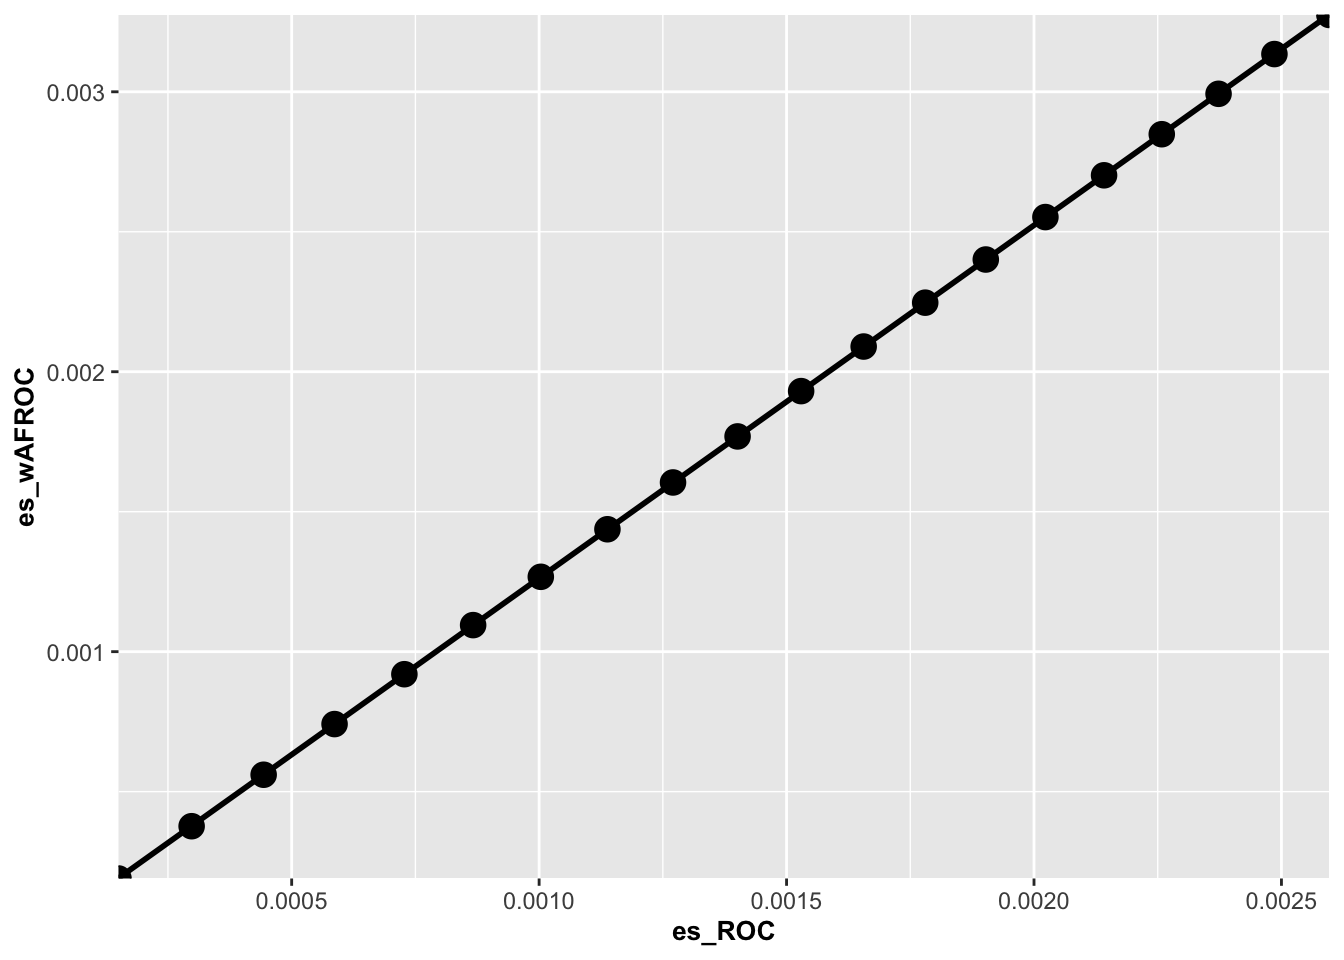
\includegraphics{18b-froc-sample-size_files/figure-latex/unnamed-chunk-7-1} \end{center}

The plot is very close to linear. This makes it easy to design an interpolation function. In the following code block the first line fits \texttt{eswAfroc} vs.~\texttt{esRoc} using the linear model \texttt{lm()} function constrained to pass through the origin (the minus one): \texttt{scaleFactor\ \textless{}-\ lm(eswAfroc\ \textasciitilde{}\ -1\ +\ esRoc)}. One expects this constraint since for \texttt{deltaMu\ =\ 0} the effect size must be zero no matter how it is measured.

\begin{Shaded}
\begin{Highlighting}[]
\NormalTok{scaleFactor<-}\KeywordTok{lm}\NormalTok{(eswAfroc}\OperatorTok{~-}\DecValTok{1}\OperatorTok{+}\NormalTok{esRoc) }\CommentTok{# fit values to straight line thru origin}
\NormalTok{effectSizeROC <-}\StringTok{ }\KeywordTok{seq}\NormalTok{(}\FloatTok{0.01}\NormalTok{, }\FloatTok{0.1}\NormalTok{, }\FloatTok{0.01}\NormalTok{)}
\NormalTok{effectSizewAFROC <-}\StringTok{ }\NormalTok{effectSizeROC}\OperatorTok{*}\NormalTok{scaleFactor}\OperatorTok{$}\NormalTok{coefficients[}\DecValTok{1}\NormalTok{] }\CommentTok{# r2 = summary(scaleFactor)$r.squared}
\end{Highlighting}
\end{Shaded}

The slope of the zero-intercept constrained straight line fit is \texttt{scaleFactor} = 1.2617239 and the squared correlation coefficient is \texttt{R2} = 0.9999997. Therefore, the conversion from ROC to wAFROC effect size is: \texttt{effectSizewAFROC\ =\ scaleFactor\ *\ effectSizeROC}. \textbf{The wAFROC effect size is twice the ROC effect size.} All that remains is to calculate the variance components using the two FOMs.

\hypertarget{computing-the-respective-variance-components}{%
\subsection{Computing the respective variance components}\label{computing-the-respective-variance-components}}

The code block applies \texttt{StSignificanceTesting()} to \texttt{rocData} and \texttt{frocData}, using the appropriate FOM, and extracts the variance components.

\begin{Shaded}
\begin{Highlighting}[]
\NormalTok{temp1 <-}\StringTok{ }\KeywordTok{StSignificanceTesting}\NormalTok{(rocData, }\DataTypeTok{FOM =} \StringTok{"Wilcoxon"}\NormalTok{, }\DataTypeTok{method =} \StringTok{"DBM"}\NormalTok{, }\DataTypeTok{analysisOption =} \StringTok{"RRRC"}\NormalTok{)}
\NormalTok{temp2 <-}\StringTok{ }\KeywordTok{StSignificanceTesting}\NormalTok{(frocData, }\DataTypeTok{FOM =} \StringTok{"wAFROC"}\NormalTok{, }\DataTypeTok{method =} \StringTok{"DBM"}\NormalTok{, }\DataTypeTok{analysisOption =} \StringTok{"RRRC"}\NormalTok{)}
\NormalTok{varCompROC <-}\StringTok{ }\NormalTok{temp1}\OperatorTok{$}\NormalTok{ANOVA}\OperatorTok{$}\NormalTok{VarCom}
\NormalTok{varCompwAFROC <-}\StringTok{ }\NormalTok{temp2}\OperatorTok{$}\NormalTok{ANOVA}\OperatorTok{$}\NormalTok{VarCom}
\end{Highlighting}
\end{Shaded}

The observed wAFROC effect-size is -0.00685625. This is a very small effect size; the corresponding ROC effect-size is -0.0051; the sign does not affect the calculations, which is too small to reach 80\% power. It is not surprising that the study \citep{RN1882} did not find a significant difference between these two treatments

The respective variance components are:

\begin{Shaded}
\begin{Highlighting}[]
\KeywordTok{print}\NormalTok{(varCompROC)}
\end{Highlighting}
\end{Shaded}

\begin{verbatim}
##            Estimates
## VarR   0.00082773798
## VarC   0.03812334734
## VarTR  0.00015265067
## VarTC  0.00964432675
## VarRC  0.00354419640
## VarErr 0.09484636574
\end{verbatim}

\begin{Shaded}
\begin{Highlighting}[]
\KeywordTok{print}\NormalTok{(varCompwAFROC)}
\end{Highlighting}
\end{Shaded}

\begin{verbatim}
##             Estimates
## VarR    0.00185422886
## VarC    0.06117804981
## VarTR  -0.00044392794
## VarTC   0.01016518621
## VarRC   0.01355883396
## VarErr  0.09672559908
\end{verbatim}

Only terms involving treatment are relevant to sample size. The wAFROC \texttt{varTC} and \texttt{varErr} values are slightly larger than the ROC ones - as expected - because the range of the wAFROC FOM is twice that of the ROC FOM.

\hypertarget{comparing-roc-power-to-wafroc-power-for-equivalent-effect-sizes}{%
\subsection{Comparing ROC power to wAFROC power for equivalent effect-sizes}\label{comparing-roc-power-to-wafroc-power-for-equivalent-effect-sizes}}

We are now ready to compare ROC and wAFROC powers for equivalent effect sizes. The following example is for 5 readers (\texttt{JPivot}) and 100 cases (\texttt{KPivot}) in the \textbf{pivotal study}.

\begin{Shaded}
\begin{Highlighting}[]
\NormalTok{powerROC <-}\StringTok{ }\KeywordTok{array}\NormalTok{(}\DataTypeTok{dim =} \KeywordTok{length}\NormalTok{(effectSizeROC));powerwAFROC <-}\StringTok{ }\KeywordTok{array}\NormalTok{(}\DataTypeTok{dim =} \KeywordTok{length}\NormalTok{(effectSizeROC))}

\NormalTok{JPivot <-}\StringTok{ }\DecValTok{5}\NormalTok{;KPivot <-}\StringTok{ }\DecValTok{100}
\ControlFlowTok{for}\NormalTok{ (i }\ControlFlowTok{in} \DecValTok{1}\OperatorTok{:}\KeywordTok{length}\NormalTok{(effectSizeROC)) \{}
\NormalTok{  varYTR <-}\StringTok{ }\NormalTok{varCompROC[}\StringTok{"VarTR"}\NormalTok{,}\StringTok{"Estimates"}\NormalTok{] }\CommentTok{# these are pseudovalue based variance components assuming FOM = "Wilcoxon"}
\NormalTok{  varYTC <-}\StringTok{ }\NormalTok{varCompROC[}\StringTok{"VarTC"}\NormalTok{,}\StringTok{"Estimates"}\NormalTok{]}
\NormalTok{  varYEps <-}\StringTok{ }\NormalTok{varCompROC[}\StringTok{"VarErr"}\NormalTok{,}\StringTok{"Estimates"}\NormalTok{]}
\NormalTok{  ret <-}\StringTok{ }\KeywordTok{SsPowerGivenJK}\NormalTok{(}\DataTypeTok{dataset =} \OtherTok{NULL}\NormalTok{, }\DataTypeTok{FOM =} \StringTok{"Wilcoxon"}\NormalTok{, }\DataTypeTok{J =}\NormalTok{ JPivot, }\DataTypeTok{K =}\NormalTok{ KPivot, }\DataTypeTok{analysisOption =} \StringTok{"RRRC"}\NormalTok{, }\DataTypeTok{effectSize =}\NormalTok{ effectSizeROC[i], }\DataTypeTok{method =} \StringTok{"DBM"}\NormalTok{, }\DataTypeTok{LegacyCode =} \OtherTok{TRUE}\NormalTok{, }
        \KeywordTok{list}\NormalTok{(}\DataTypeTok{VarTR =}\NormalTok{ varYTR, }\DataTypeTok{VarTC =}\NormalTok{ varYTC, }\DataTypeTok{VarErr =}\NormalTok{ varYEps))}
\NormalTok{  powerROC[i] <-}\StringTok{ }\NormalTok{ret}\OperatorTok{$}\NormalTok{powerRRRC}
  
\NormalTok{  varYTR <-}\StringTok{ }\NormalTok{varCompwAFROC[}\StringTok{"VarTR"}\NormalTok{,}\StringTok{"Estimates"}\NormalTok{] }\CommentTok{# these are pseudovalue based variance components assuming FOM = "wAFROC"}
\NormalTok{  varYTC <-}\StringTok{ }\NormalTok{varCompwAFROC[}\StringTok{"VarTC"}\NormalTok{,}\StringTok{"Estimates"}\NormalTok{]}
\NormalTok{  varYEps <-}\StringTok{ }\NormalTok{varCompwAFROC[}\StringTok{"VarErr"}\NormalTok{,}\StringTok{"Estimates"}\NormalTok{]}
\NormalTok{  ret <-}\StringTok{ }\KeywordTok{SsPowerGivenJK}\NormalTok{(}\DataTypeTok{dataset =} \OtherTok{NULL}\NormalTok{, }\DataTypeTok{FOM =} \StringTok{"Wilcoxon"}\NormalTok{, }\DataTypeTok{J =}\NormalTok{ JPivot, }\DataTypeTok{K =}\NormalTok{ KPivot, }\DataTypeTok{analysisOption =} \StringTok{"RRRC"}\NormalTok{, }\DataTypeTok{effectSize =}\NormalTok{ effectSizewAFROC[i], }\DataTypeTok{method =} \StringTok{"DBM"}\NormalTok{, }\DataTypeTok{LegacyCode =} \OtherTok{TRUE}\NormalTok{, }
        \KeywordTok{list}\NormalTok{(}\DataTypeTok{VarTR =}\NormalTok{ varYTR, }\DataTypeTok{VarTC =}\NormalTok{ varYTC, }\DataTypeTok{VarErr =}\NormalTok{ varYEps))}
\NormalTok{  powerwAFROC[i] <-}\StringTok{ }\NormalTok{ret}\OperatorTok{$}\NormalTok{powerRRRC}
  
  \KeywordTok{cat}\NormalTok{(}\StringTok{"ROC-ES = "}\NormalTok{, effectSizeROC[i], }\StringTok{", wAFROC-ES = "}\NormalTok{, effectSizewAFROC[i], }
      \StringTok{", Power-ROC = "}\NormalTok{, powerROC[i], }\StringTok{", Power-wAFROC = "}\NormalTok{, powerwAFROC[i], }\StringTok{"}\CharTok{\textbackslash{}n}\StringTok{"}\NormalTok{)}
\NormalTok{\}}
\end{Highlighting}
\end{Shaded}

\begin{verbatim}
## ROC-ES =  0.01 , wAFROC-ES =  0.012617239 , Power-ROC =  0.064430457 , Power-wAFROC =  0.075439644 
## ROC-ES =  0.02 , wAFROC-ES =  0.025234479 , Power-ROC =  0.10878897 , Power-wAFROC =  0.15449773 
## ROC-ES =  0.03 , wAFROC-ES =  0.037851718 , Power-ROC =  0.18471152 , Power-wAFROC =  0.28797922 
## ROC-ES =  0.04 , wAFROC-ES =  0.050468957 , Power-ROC =  0.29079274 , Power-wAFROC =  0.4612966 
## ROC-ES =  0.05 , wAFROC-ES =  0.063086196 , Power-ROC =  0.41954431 , Power-wAFROC =  0.6420946 
## ROC-ES =  0.06 , wAFROC-ES =  0.075703436 , Power-ROC =  0.55738123 , Power-wAFROC =  0.79495349 
## ROC-ES =  0.07 , wAFROC-ES =  0.088320675 , Power-ROC =  0.68816012 , Power-wAFROC =  0.90003872 
## ROC-ES =  0.08 , wAFROC-ES =  0.10093791 , Power-ROC =  0.79836108 , Power-wAFROC =  0.95891383 
## ROC-ES =  0.09 , wAFROC-ES =  0.11355515 , Power-ROC =  0.88095077 , Power-wAFROC =  0.98585038 
## ROC-ES =  0.1 , wAFROC-ES =  0.12617239 , Power-ROC =  0.93606799 , Power-wAFROC =  0.9959336
\end{verbatim}

Since the wAFROC effect size is about a factor of two larger than the ROC effect size, wAFROC power is larger than that for ROC. The effect is magnified as the effect size enters as the square in the formula for the power (this overwhelms the slight increase in variability of wAFROC-FOM relative to ROC-FOM noted previously). The following is a plot of the respective powers.

\begin{Shaded}
\begin{Highlighting}[]
\NormalTok{df <-}\StringTok{ }\KeywordTok{data.frame}\NormalTok{(}\DataTypeTok{power_ROC =}\NormalTok{ powerROC, }\DataTypeTok{power_wAFROC =}\NormalTok{ powerwAFROC)}
\NormalTok{p <-}\StringTok{ }\KeywordTok{ggplot}\NormalTok{(}\DataTypeTok{mapping =} \KeywordTok{aes}\NormalTok{(}\DataTypeTok{x =}\NormalTok{ power_ROC, }\DataTypeTok{y =}\NormalTok{ power_wAFROC)) }\OperatorTok{+}
\StringTok{  }\KeywordTok{geom_line}\NormalTok{(}\DataTypeTok{data =}\NormalTok{ df, }\DataTypeTok{size =} \DecValTok{2}\NormalTok{)}\OperatorTok{+}
\StringTok{  }\KeywordTok{scale_color_manual}\NormalTok{(}\DataTypeTok{values =} \StringTok{"black"}\NormalTok{) }\OperatorTok{+}\StringTok{ }
\StringTok{  }\KeywordTok{theme}\NormalTok{(}\DataTypeTok{axis.title.y =} \KeywordTok{element_text}\NormalTok{(}\DataTypeTok{size =} \DecValTok{10}\NormalTok{,}\DataTypeTok{face=}\StringTok{"bold"}\NormalTok{),}
        \DataTypeTok{axis.title.x =} \KeywordTok{element_text}\NormalTok{(}\DataTypeTok{size =} \DecValTok{10}\NormalTok{,}\DataTypeTok{face=}\StringTok{"bold"}\NormalTok{))  }\OperatorTok{+}
\StringTok{  }\KeywordTok{scale_x_continuous}\NormalTok{(}\DataTypeTok{expand =} \KeywordTok{c}\NormalTok{(}\DecValTok{0}\NormalTok{, }\DecValTok{0}\NormalTok{)) }\OperatorTok{+}\StringTok{ }
\StringTok{  }\KeywordTok{scale_y_continuous}\NormalTok{(}\DataTypeTok{expand =} \KeywordTok{c}\NormalTok{(}\DecValTok{0}\NormalTok{, }\DecValTok{0}\NormalTok{))}
\KeywordTok{print}\NormalTok{(p)}
\end{Highlighting}
\end{Shaded}

\begin{center}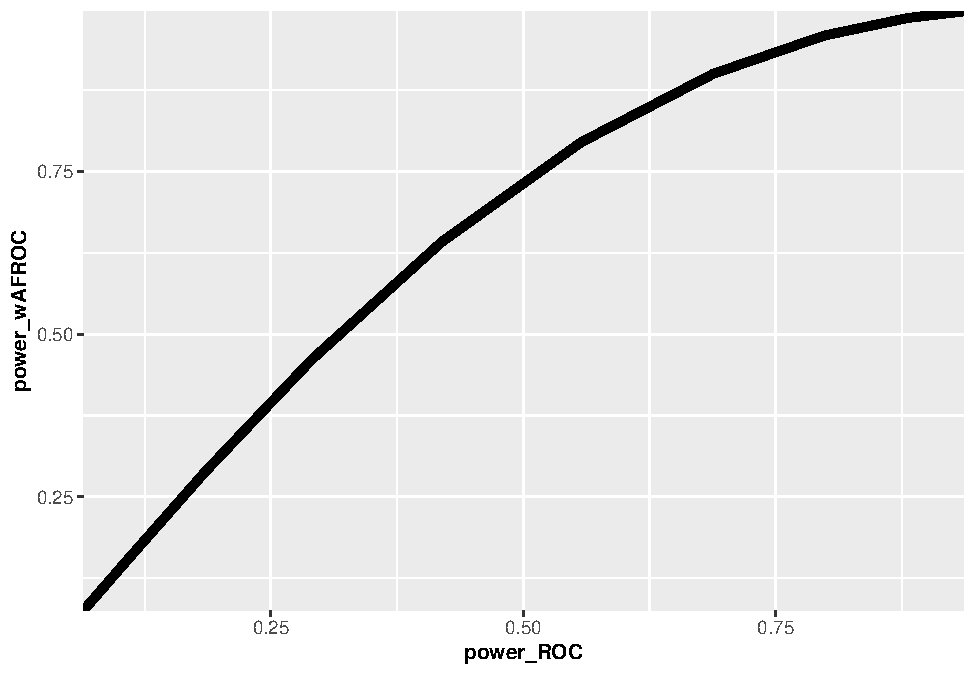
\includegraphics{18b-froc-sample-size_files/figure-latex/unnamed-chunk-12-1} \end{center}

\hypertarget{part-2}{%
\section{Part 2}\label{part-2}}

\hypertarget{introduction}{%
\subsection{Introduction}\label{introduction}}

This example uses the FED dataset as a pilot FROC study and function \texttt{SsFrocNhRsmModel()} to construct the NH model (encapsulating some of the code in the first part).

\hypertarget{constructing-the-nh-model-for-the-dataset}{%
\subsection{Constructing the NH model for the dataset}\label{constructing-the-nh-model-for-the-dataset}}

One starts by extracting the first two treatments from \texttt{dataset04}, which represent the NH dataset, see previous part. Next one constructs the NH model - note that the lesion distribution \texttt{lesDistr} can be specified here independently of that in the pilot dataset. This allows some control over selection of the diseased cases in the pivotal study.

\begin{Shaded}
\begin{Highlighting}[]
\NormalTok{lesDistr <-}\StringTok{ }\KeywordTok{c}\NormalTok{(}\FloatTok{0.7}\NormalTok{, }\FloatTok{0.2}\NormalTok{, }\FloatTok{0.1}\NormalTok{)}
\NormalTok{frocNhData <-}\StringTok{ }\KeywordTok{DfExtractDataset}\NormalTok{(dataset04, }\DataTypeTok{trts =} \KeywordTok{c}\NormalTok{(}\DecValTok{1}\NormalTok{,}\DecValTok{2}\NormalTok{))}
\NormalTok{ret <-}\StringTok{ }\KeywordTok{SsFrocNhRsmModel}\NormalTok{(frocNhData, }\DataTypeTok{lesDistr =}\NormalTok{ lesDistr)}
\NormalTok{mu <-}\StringTok{ }\NormalTok{ret}\OperatorTok{$}\NormalTok{mu}
\NormalTok{lambda <-}\StringTok{ }\NormalTok{ret}\OperatorTok{$}\NormalTok{lambda}
\NormalTok{nu <-}\StringTok{ }\NormalTok{ret}\OperatorTok{$}\NormalTok{nu}
\NormalTok{scaleFactor <-}\StringTok{ }\NormalTok{ret}\OperatorTok{$}\NormalTok{scaleFactor}
\end{Highlighting}
\end{Shaded}

The fitting model is defined by \texttt{mu} = 3.31491361, \texttt{lambda} = 1.6930673 and \texttt{nu} = 0.70649936 and \texttt{lesDistr}. The effect size scale factor is 1.25445833.

\begin{Shaded}
\begin{Highlighting}[]
\NormalTok{aucRocNH <-}\StringTok{ }\KeywordTok{PlotRsmOperatingCharacteristics}\NormalTok{(mu, lambda, nu, }
                                            \DataTypeTok{lesDistr =}\NormalTok{ lesDistr, }\DataTypeTok{OpChType =} \StringTok{"ROC"}\NormalTok{)}\OperatorTok{$}\NormalTok{aucROC}
\NormalTok{aucwAfrocNH <-}\StringTok{ }\KeywordTok{PlotRsmOperatingCharacteristics}\NormalTok{(mu, lambda, nu, }
                                               \DataTypeTok{lesDistr =}\NormalTok{ lesDistr, }\DataTypeTok{OpChType =} \StringTok{"wAFROC"}\NormalTok{)}\OperatorTok{$}\NormalTok{aucwAFROC}
\end{Highlighting}
\end{Shaded}

The null hypothesis ROC AUC is 0.8790548 and the corresponding NH wAFROC AUC is 0.72320816.

\hypertarget{extracting-the-wafroc-variance-components}{%
\subsection{Extracting the wAFROC variance components}\label{extracting-the-wafroc-variance-components}}

The next code block applies \texttt{StSignificanceTesting()} to \texttt{frocNhData}, using \texttt{FOM\ =\ "wAFROC"} and extracts the variance components.

\begin{Shaded}
\begin{Highlighting}[]
\NormalTok{varCompwAFROC  <-}\StringTok{ }\KeywordTok{StSignificanceTesting}\NormalTok{(frocNhData, }\DataTypeTok{FOM =} \StringTok{"wAFROC"}\NormalTok{, }\DataTypeTok{method =} \StringTok{"DBM"}\NormalTok{, }\DataTypeTok{analysisOption =} \StringTok{"RRRC"}\NormalTok{)}\OperatorTok{$}\NormalTok{ANOVA}\OperatorTok{$}\NormalTok{VarCom}
\end{Highlighting}
\end{Shaded}

\hypertarget{wafroc-power-for-specified-roc-effect-size-number-of-readers-j-and-number-of-cases-k}{%
\subsection{wAFROC power for specified ROC effect size, number of readers J and number of cases K}\label{wafroc-power-for-specified-roc-effect-size-number-of-readers-j-and-number-of-cases-k}}

The following example is for ROC effect size = 0.05, 5 readers (\texttt{J\ =\ 5}) and 100 cases (\texttt{K\ =\ 100}) in the \textbf{pivotal study}.

\begin{Shaded}
\begin{Highlighting}[]
\NormalTok{ROC_ES <-}\StringTok{ }\FloatTok{0.05}
\NormalTok{effectSizewAFROC <-}\StringTok{ }\NormalTok{scaleFactor }\OperatorTok{*}\StringTok{ }\NormalTok{ROC_ES}
\NormalTok{J <-}\StringTok{ }\DecValTok{5}\NormalTok{;K <-}\StringTok{ }\DecValTok{100}

\NormalTok{varYTR <-}\StringTok{ }\NormalTok{varCompwAFROC[}\StringTok{"VarTR"}\NormalTok{,}\StringTok{"Estimates"}\NormalTok{] }
\NormalTok{varYTC <-}\StringTok{ }\NormalTok{varCompwAFROC[}\StringTok{"VarTC"}\NormalTok{,}\StringTok{"Estimates"}\NormalTok{]}
\NormalTok{varYEps <-}\StringTok{ }\NormalTok{varCompwAFROC[}\StringTok{"VarErr"}\NormalTok{,}\StringTok{"Estimates"}\NormalTok{]}
\NormalTok{ret <-}\StringTok{ }\KeywordTok{SsPowerGivenJK}\NormalTok{(}\DataTypeTok{dataset =} \OtherTok{NULL}\NormalTok{, }\DataTypeTok{FOM =} \StringTok{"Wilcoxon"}\NormalTok{, }\DataTypeTok{J =}\NormalTok{ J, }\DataTypeTok{K =}\NormalTok{ K, }\DataTypeTok{analysisOption =} \StringTok{"RRRC"}\NormalTok{, }
                      \DataTypeTok{effectSize =}\NormalTok{ effectSizewAFROC, }\DataTypeTok{method =} \StringTok{"DBM"}\NormalTok{, }\DataTypeTok{LegacyCode =} \OtherTok{TRUE}\NormalTok{, }
                      \KeywordTok{list}\NormalTok{(}\DataTypeTok{VarTR =}\NormalTok{ varYTR,}
                           \DataTypeTok{VarTC =}\NormalTok{ varYTC,}
                           \DataTypeTok{VarErr =}\NormalTok{ varYEps))}
\NormalTok{powerwAFROC <-}\StringTok{ }\NormalTok{ret}\OperatorTok{$}\NormalTok{powerRRRC}

\KeywordTok{cat}\NormalTok{(}\StringTok{"ROC-ES = "}\NormalTok{, ROC_ES, }\StringTok{", wAFROC-ES = "}\NormalTok{, ROC_ES }\OperatorTok{*}\StringTok{ }\NormalTok{scaleFactor, }\StringTok{", Power-wAFROC = "}\NormalTok{, powerwAFROC, }\StringTok{"}\CharTok{\textbackslash{}n}\StringTok{"}\NormalTok{)}
\end{Highlighting}
\end{Shaded}

\begin{verbatim}
## ROC-ES =  0.05 , wAFROC-ES =  0.062722916 , Power-wAFROC =  0.63713244
\end{verbatim}

\hypertarget{wafroc-number-of-cases-for-80-power-for-a-given-number-of-readers-j}{%
\subsection{wAFROC number of cases for 80\% power for a given number of readers J}\label{wafroc-number-of-cases-for-80-power-for-a-given-number-of-readers-j}}

\begin{Shaded}
\begin{Highlighting}[]
\NormalTok{VarTR <-}\StringTok{ }\NormalTok{varCompwAFROC[}\StringTok{"VarTR"}\NormalTok{,}\StringTok{"Estimates"}\NormalTok{] }
\NormalTok{VarTC <-}\StringTok{ }\NormalTok{varCompwAFROC[}\StringTok{"VarTC"}\NormalTok{,}\StringTok{"Estimates"}\NormalTok{]}
\NormalTok{VarErr <-}\StringTok{ }\NormalTok{varCompwAFROC[}\StringTok{"VarErr"}\NormalTok{,}\StringTok{"Estimates"}\NormalTok{]}
\NormalTok{ret2 <-}\StringTok{ }\KeywordTok{SsSampleSizeKGivenJ}\NormalTok{(}\DataTypeTok{dataset =} \OtherTok{NULL}\NormalTok{, }\DataTypeTok{J =} \DecValTok{6}\NormalTok{, }\DataTypeTok{effectSize =}\NormalTok{ effectSizewAFROC, }\DataTypeTok{method =} \StringTok{"DBM"}\NormalTok{, }\DataTypeTok{LegacyCode =} \OtherTok{TRUE}\NormalTok{,}
                            \KeywordTok{list}\NormalTok{(}\DataTypeTok{VarTR =}\NormalTok{ VarTR, }\DataTypeTok{VarTC =}\NormalTok{ VarTC, }\DataTypeTok{VarErr =}\NormalTok{ VarErr))}

\KeywordTok{cat}\NormalTok{(}\StringTok{"ROC-ES = "}\NormalTok{, ROC_ES, }\StringTok{", wAFROC-ES = "}\NormalTok{, ROC_ES }\OperatorTok{*}\StringTok{ }\NormalTok{scaleFactor, }
    \StringTok{", K80RRRC = "}\NormalTok{, ret2}\OperatorTok{$}\NormalTok{KRRRC, }\StringTok{", Power-wAFROC = "}\NormalTok{, ret2}\OperatorTok{$}\NormalTok{powerRRRC, }\StringTok{"}\CharTok{\textbackslash{}n}\StringTok{"}\NormalTok{)}
\end{Highlighting}
\end{Shaded}

\begin{verbatim}
## ROC-ES =  0.05 , wAFROC-ES =  0.062722916 , K80RRRC =  123 , Power-wAFROC =  0.80210887
\end{verbatim}

\hypertarget{wafroc-fom-power-for-a-given-number-of-readers-j-and-cases-k}{%
\subsection{wAFROC-FOM power for a given number of readers J and cases K}\label{wafroc-fom-power-for-a-given-number-of-readers-j-and-cases-k}}

\begin{Shaded}
\begin{Highlighting}[]
\NormalTok{ret3 <-}\StringTok{ }\KeywordTok{SsPowerGivenJK}\NormalTok{(}\DataTypeTok{dataset =} \OtherTok{NULL}\NormalTok{, }\DataTypeTok{J =} \DecValTok{6}\NormalTok{, }\DataTypeTok{K =}\NormalTok{ ret2}\OperatorTok{$}\NormalTok{KRRRC, }\DataTypeTok{effectSize =}\NormalTok{ effectSizewAFROC, }\DataTypeTok{method =} \StringTok{"DBM"}\NormalTok{, }\DataTypeTok{LegacyCode =} \OtherTok{TRUE}\NormalTok{,}
                       \KeywordTok{list}\NormalTok{(}\DataTypeTok{VarTR =}\NormalTok{ VarTR, }\DataTypeTok{VarTC =}\NormalTok{ VarTC, }\DataTypeTok{VarErr =}\NormalTok{ VarErr))}

\KeywordTok{cat}\NormalTok{(}\StringTok{"ROC-ES = "}\NormalTok{, ROC_ES, }\StringTok{", wAFROC-ES = "}\NormalTok{, ROC_ES }\OperatorTok{*}\StringTok{ }\NormalTok{scaleFactor, }
    \StringTok{", powerRRRC = "}\NormalTok{, ret3}\OperatorTok{$}\NormalTok{powerRRRC, }\StringTok{"}\CharTok{\textbackslash{}n}\StringTok{"}\NormalTok{)}
\end{Highlighting}
\end{Shaded}

\begin{verbatim}
## ROC-ES =  0.05 , wAFROC-ES =  0.062722916 , powerRRRC =  0.80210887
\end{verbatim}

The estimated power is close to 80\% as the number of cases (\texttt{ret2\$KRRRC\ =\ 123}) was chosen deliberately from the previous code block.

\hypertarget{froc-sample-size-references}{%
\section{References}\label{froc-sample-size-references}}

\hypertarget{part-rjafroc-vignettes}{%
\part*{RJafroc Vignettes}\label{part-rjafroc-vignettes}}
\addcontentsline{toc}{part}{RJafroc Vignettes}

\hypertarget{background-f-distribution}{%
\chapter{F-distribution}\label{background-f-distribution}}

\hypertarget{background-f-distribution-how-much-finished}{%
\section{TBA How much finished}\label{background-f-distribution-how-much-finished}}

10\%

\hypertarget{background}{%
\section{Background}\label{background}}

A number of vignettes used to be part of the \texttt{RJafroc} package. These have been moved here.

\hypertarget{introduction-1}{%
\section{Introduction}\label{introduction-1}}

Since it plays an important role in sample size estimation, it is helpful to examine the behavior of the F-distribution. In the following \texttt{ndf} = numerator degrees of freedom, \texttt{ddf} = denominator degrees of freedom and \texttt{ncp} = non-centrality parameter (i.e., the \(\Delta\) appearing in Eqn. (11.6) of \citep{chakraborty2017observer}).

The use of three \texttt{R} functions is demonstrated.

\begin{itemize}
\item
  \texttt{qf(p,ndf,ddf)} is the \emph{quantile} function of the F-distribution for specified values of \texttt{p}, \texttt{ndf} and \texttt{ddf}, i.e., the value \texttt{x} such that fraction \texttt{p} of the area under the F-distribution lies to the right of \texttt{x}. Since \texttt{ncp} is not included as a parameter, the default value, i.e., zero, is used. This is called the \emph{central} F-distribution.
\item
  \texttt{df(x,ndf,ddf,ncp)} is the probability density function (\emph{pdf}) of the F-distribution, as a function of \texttt{x}, for specified values of \texttt{ndf}, \texttt{ddf} and \texttt{ncp}.
\item
  \texttt{pf(x,ndf,ddf,ncp)} is the probability (or cumulative) distribution function of the F-distribution for specified values of \texttt{ndf}, \texttt{ddf} and \texttt{ncp}.
\end{itemize}

\hypertarget{effect-of-ncp-for-ndf-2-and-ddf-10}{%
\section{\texorpdfstring{Effect of \texttt{ncp} for \texttt{ndf} = 2 and \texttt{ddf} = 10}{Effect of ncp for ndf = 2 and ddf = 10}}\label{effect-of-ncp-for-ndf-2-and-ddf-10}}

\begin{itemize}
\tightlist
\item
  Four values of \texttt{ncp} are considered (0, 2, 5, 10) for \texttt{ddf} = 10.
\item
  \texttt{fCrit} is the critical value of the F distribution, i.e., that value such that fraction \(\alpha\) of the area is to the right of the critical value, i.e., \texttt{fCrit} is identical in statistical notation to \({{F}_{1-\alpha ,ndf,ddf}}\).
\end{itemize}

\begin{Shaded}
\begin{Highlighting}[]
\NormalTok{ndf <-}\StringTok{ }\DecValTok{2}\NormalTok{;ddf <-}\StringTok{ }\DecValTok{10}\NormalTok{;ncp <-}\StringTok{ }\KeywordTok{c}\NormalTok{(}\DecValTok{0}\NormalTok{,}\DecValTok{2}\NormalTok{,}\DecValTok{5}\NormalTok{,}\DecValTok{10}\NormalTok{)}
\NormalTok{alpha <-}\StringTok{ }\FloatTok{0.05}
\NormalTok{fCrit <-}\StringTok{ }\KeywordTok{qf}\NormalTok{(}\DecValTok{1}\OperatorTok{-}\NormalTok{alpha, ndf,ddf)}
\NormalTok{x <-}\StringTok{ }\KeywordTok{seq}\NormalTok{(}\DecValTok{1}\NormalTok{, }\DecValTok{20}\NormalTok{, }\FloatTok{0.1}\NormalTok{)}
\NormalTok{myLabel <-}\StringTok{ }\KeywordTok{c}\NormalTok{(}\StringTok{"A"}\NormalTok{, }\StringTok{"B"}\NormalTok{, }\StringTok{"C"}\NormalTok{, }\StringTok{"D"}\NormalTok{)}
\NormalTok{myLabelIndx <-}\StringTok{ }\DecValTok{1}
\NormalTok{pFgtFCrit <-}\StringTok{ }\OtherTok{NULL}
\ControlFlowTok{for}\NormalTok{ (i }\ControlFlowTok{in} \DecValTok{1}\OperatorTok{:}\KeywordTok{length}\NormalTok{(ncp))}
\NormalTok{\{}
\NormalTok{  y <-}\StringTok{ }\KeywordTok{df}\NormalTok{(x,ndf,ddf,}\DataTypeTok{ncp=}\NormalTok{ncp[i])}
\NormalTok{  pFgtFCrit <-}\StringTok{ }\KeywordTok{c}\NormalTok{(pFgtFCrit, }\DecValTok{1}\OperatorTok{-}\KeywordTok{pf}\NormalTok{(fCrit, ndf, ddf, }\DataTypeTok{ncp =}\NormalTok{ ncp[i]))}
\NormalTok{\}  }
\ControlFlowTok{for}\NormalTok{ (i }\ControlFlowTok{in} \DecValTok{1}\OperatorTok{:}\KeywordTok{length}\NormalTok{(ncp))}
\NormalTok{\{}
\NormalTok{  y <-}\StringTok{ }\KeywordTok{df}\NormalTok{(x,ndf,ddf,}\DataTypeTok{ncp=}\NormalTok{ncp[i])}
\NormalTok{  curveData <-}\StringTok{ }\KeywordTok{data.frame}\NormalTok{(}\DataTypeTok{x =}\NormalTok{ x, }\DataTypeTok{pdf =}\NormalTok{ y)}
\NormalTok{  curvePlot <-}\StringTok{ }\KeywordTok{ggplot}\NormalTok{(}\DataTypeTok{data =}\NormalTok{ curveData, }\DataTypeTok{mapping =} \KeywordTok{aes}\NormalTok{(}\DataTypeTok{x =}\NormalTok{ x, }\DataTypeTok{y =}\NormalTok{ pdf)) }\OperatorTok{+}\StringTok{ }
\StringTok{    }\KeywordTok{geom_line}\NormalTok{() }\OperatorTok{+}
\StringTok{    }\KeywordTok{ggtitle}\NormalTok{(myLabel[myLabelIndx]);myLabelIndx <-}\StringTok{ }\NormalTok{myLabelIndx }\OperatorTok{+}\StringTok{ }\DecValTok{1}
  \KeywordTok{print}\NormalTok{(curvePlot)}
\NormalTok{\}}
\NormalTok{fCrit_}\DecValTok{2}\NormalTok{_}\DecValTok{10}\NormalTok{ <-}\StringTok{ }\NormalTok{fCrit }\CommentTok{# convention fCrit_ndf_ddf}
\end{Highlighting}
\end{Shaded}

\includegraphics{19a-fdistribution_files/figure-latex/unnamed-chunk-1-1.pdf} 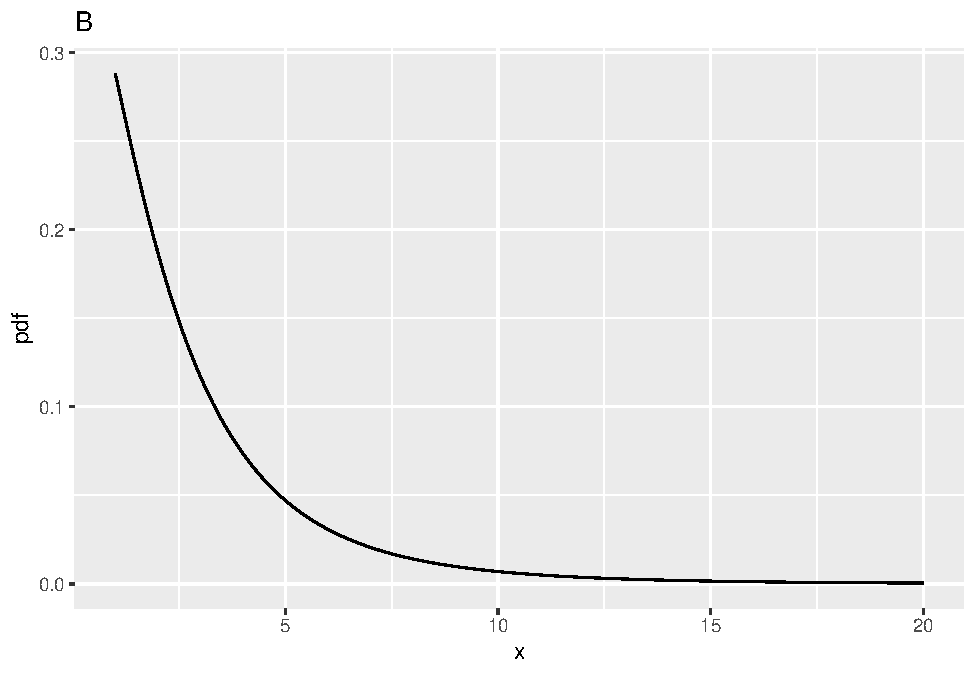
\includegraphics{19a-fdistribution_files/figure-latex/unnamed-chunk-1-2.pdf} 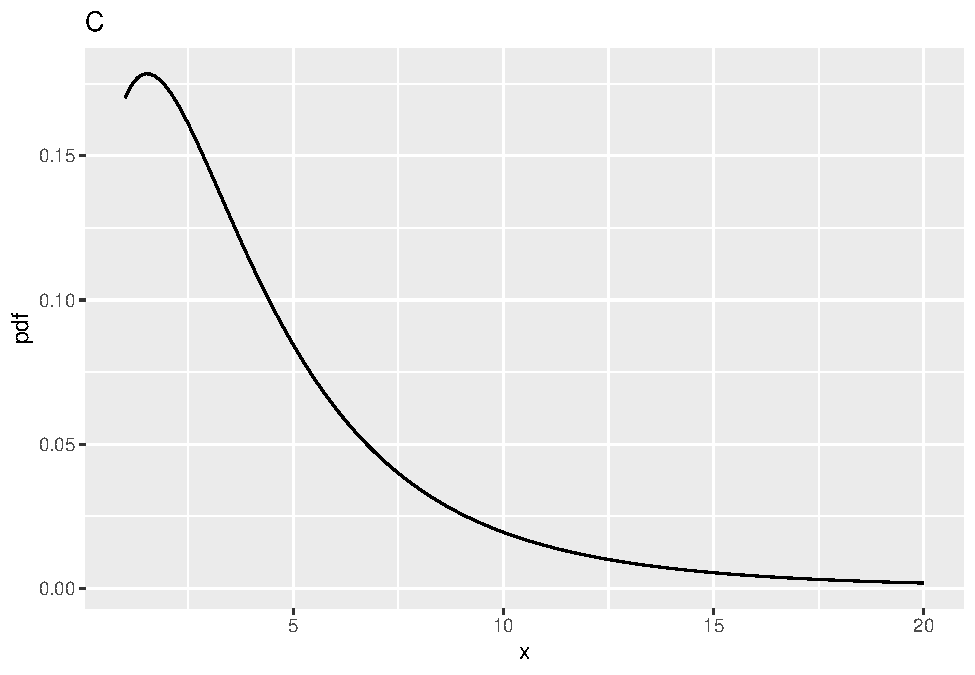
\includegraphics{19a-fdistribution_files/figure-latex/unnamed-chunk-1-3.pdf} 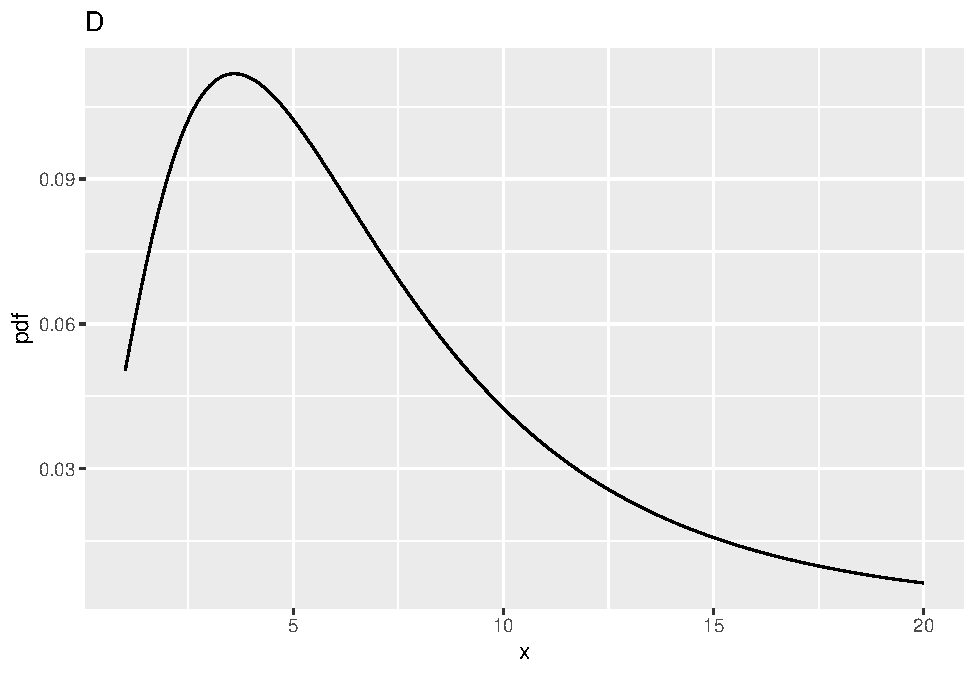
\includegraphics{19a-fdistribution_files/figure-latex/unnamed-chunk-1-4.pdf}

\begin{tabular}{l|r|r|r|r|r}
\hline
  & ndf & ddf & fCrit & ncp & pFgtFCrit\\
\hline
A & 2 & 10 & 4.102821 & 0 & 0.0500000\\
\hline
B & 2 & 10 & 4.102821 & 2 & 0.1775840\\
\hline
C & 2 & 10 & 4.102821 & 5 & 0.3876841\\
\hline
D & 2 & 10 & 4.102821 & 10 & 0.6769776\\
\hline
\end{tabular}

\hypertarget{comments}{%
\section{Comments}\label{comments}}

\hypertarget{fig.-a}{%
\subsection{Fig. A}\label{fig.-a}}

\begin{itemize}
\tightlist
\item
  This corresponds to \texttt{ncp\ =\ 0}, i.e., the \emph{central} F-distribution.
\item
  The integral under this distribution is unity (this is also true for all plots in this vignette).
\item
  The critical value, \texttt{fCrit} in the above code block, is the value of \texttt{x} such that the probability of exceeding \texttt{x} is \(\alpha\). The corresponding parameter \texttt{alpha} is defined above as 0.05.
\item
  In the current example \texttt{fCrit} = 4.102821. Notice the use of the quantile function \texttt{qf()} to determine this value, and the default value of \texttt{ncp}, namely zero, is used; specifically, one does not pass a 4th argument to \texttt{qf()}.
\item
  \textbf{The decision rule for rejecting the NH uses the NH distribution of the F-statistic}, i.e., reject the NH if F \textgreater= \texttt{fCrit}. As expected, \texttt{prob\ \textgreater{}\ fCrit} = 0.05 because this is how \texttt{fCrit} was defined.
\end{itemize}

\hypertarget{fig.-b}{%
\subsection{Fig. B}\label{fig.-b}}

\begin{itemize}
\tightlist
\item
  This corresponds to \texttt{ncp\ =\ 2}, \texttt{ndf} = 2 and \texttt{ddf} = 10.
\item
  The distribution is slightly shifted to the right as compared to Fig. A, thereby making it more likely that the observed value of the F-statistic will exceed the critical value determined for the NH distribution.
\item
  In fact, \texttt{prob\ \textgreater{}\ fCrit} = 0.177584, i.e., the \emph{statistical power} (compare this to Fig. A where \texttt{prob\ \textgreater{}\ fCrit} was 0.05).
\end{itemize}

\hypertarget{fig.-c}{%
\subsection{Fig. C}\label{fig.-c}}

\begin{itemize}
\tightlist
\item
  This corresponds to \texttt{ncp\ =\ 5}, \texttt{ndf} = 2 and \texttt{ddf} = 10.
\item
  Now \texttt{prob\ \textgreater{}\ fCrit} = 0.3876841.
\item
  Power has increased compared to Fig. B.
\end{itemize}

\hypertarget{fig.-d}{%
\subsection{Fig. D}\label{fig.-d}}

\begin{itemize}
\tightlist
\item
  This corresponds to \texttt{ncp\ =\ 10}, \texttt{ndf} = 2 and \texttt{ddf} = 10.
\item
  Now \texttt{prob\ \textgreater{}\ fCrit} is 0.6769776.
\item
  Power has increased compared to Fig. C.
\item
  The effect of the shift is most obvious in Fig. C and Fig. D.
\item
  Considering a vertical line at \texttt{x} = 4.102821, fraction 0.6769776 of the probability distribution in Fig. D lies to the right of this line
\item
  Therefore the NH is likely to be rejected with probability 0.6769776.
\end{itemize}

\hypertarget{summary}{%
\subsection{Summary}\label{summary}}

The larger that non-centrality parameter, the greater the shift to the right of the F-distribution, and the greater the statistical power.

\hypertarget{effect-of-ncp-for-ndf-2-and-ddf-100}{%
\section{\texorpdfstring{Effect of \texttt{ncp} for \texttt{ndf} = 2 and \texttt{ddf} = 100}{Effect of ncp for ndf = 2 and ddf = 100}}\label{effect-of-ncp-for-ndf-2-and-ddf-100}}

\includegraphics{19a-fdistribution_files/figure-latex/unnamed-chunk-3-1.pdf} \includegraphics{19a-fdistribution_files/figure-latex/unnamed-chunk-3-2.pdf} 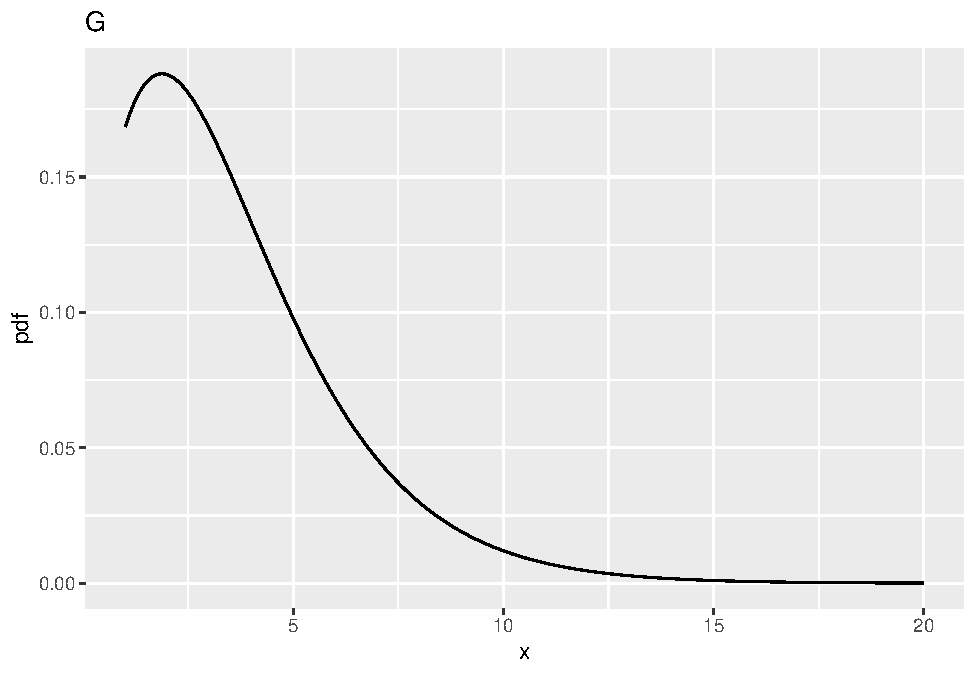
\includegraphics{19a-fdistribution_files/figure-latex/unnamed-chunk-3-3.pdf} 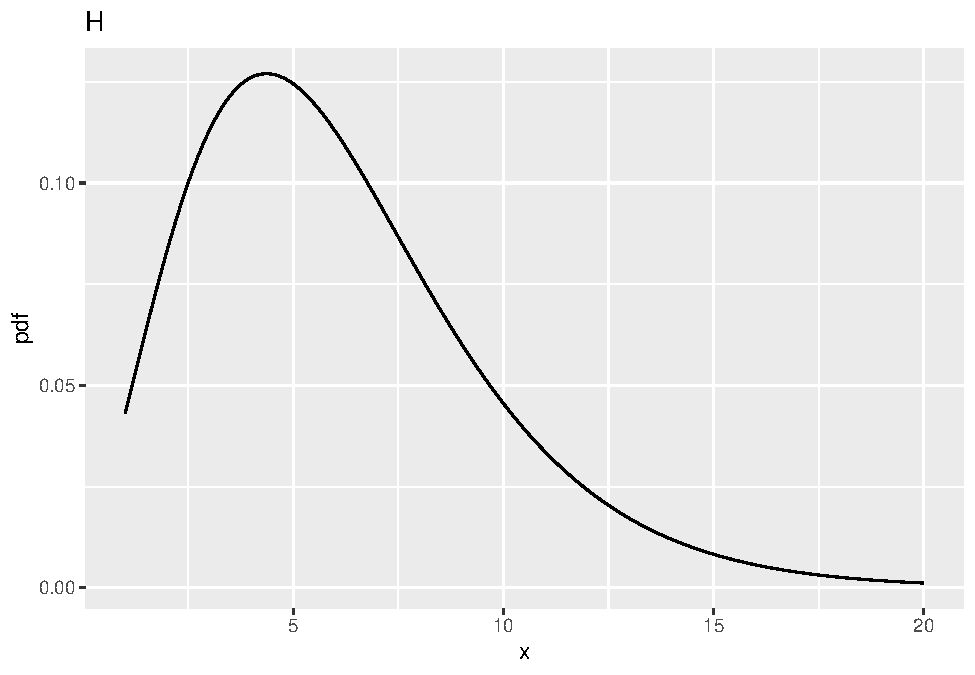
\includegraphics{19a-fdistribution_files/figure-latex/unnamed-chunk-3-4.pdf}

\begin{tabular}{l|r|r|r|r|r}
\hline
  & ndf & ddf & fCrit & ncp & pFgtFCrit\\
\hline
A & 2 & 10 & 4.102821 & 0 & 0.0500000\\
\hline
B & 2 & 10 & 4.102821 & 2 & 0.1775840\\
\hline
C & 2 & 10 & 4.102821 & 5 & 0.3876841\\
\hline
D & 2 & 10 & 4.102821 & 10 & 0.6769776\\
\hline
E & 2 & 100 & 3.087296 & 0 & 0.0500000\\
\hline
F & 2 & 100 & 3.087296 & 2 & 0.2199264\\
\hline
G & 2 & 100 & 3.087296 & 5 & 0.4910802\\
\hline
H & 2 & 100 & 3.087296 & 10 & 0.8029764\\
\hline
\end{tabular}

\hypertarget{comments-1}{%
\section{Comments}\label{comments-1}}

\begin{itemize}
\tightlist
\item
  All comparisons in this sections are at the same values of \texttt{ncp} defined above.
\item
  And between \texttt{ddf} = 100 and \texttt{ddf} = 10.
\end{itemize}

\hypertarget{fig.-e}{%
\subsection{Fig. E}\label{fig.-e}}

\begin{itemize}
\tightlist
\item
  This corresponds to \texttt{ncp} = 0, \texttt{ndf} = 2 and \texttt{ddf} = 100.
\item
  The critical value is \texttt{fCrit\_2\_100} = 3.0872959. Notice the decrease compared to the previous value for \texttt{ncp} = 0, i.e., 4.102821, for \texttt{ddf} = 10.
\item
  One expects that increasing \texttt{ddf} will make it more likely that the NH will be rejected, and this is confirmed below.
\item
  All else equal, statistical power increases with increasing \texttt{ddf}.
\end{itemize}

\hypertarget{fig.-f}{%
\subsection{Fig. F}\label{fig.-f}}

\begin{itemize}
\tightlist
\item
  This corresponds to \texttt{ncp} = 2, \texttt{ndf} = 2 and \texttt{ddf} = 100.
\item
  The probability of exceeding the critical value is \texttt{prob\ \textgreater{}\ fCrit\_2\_100} = 0.2199264, greater than the previous value, i.e., 0.177584 for \texttt{ddf} = 10.
\end{itemize}

\hypertarget{fig.-g}{%
\subsection{Fig. G}\label{fig.-g}}

\begin{itemize}
\tightlist
\item
  This corresponds to \texttt{ncp\ =\ 5}, \texttt{ndf} = 2 and \texttt{ddf} = 100.
\item
  The probability of exceeding the critical value is \texttt{prob\ \textgreater{}\ fCrit\_2\_100} = 0.4910802.
\item
  This is greater than the previous value, i.e., 0.3876841 for \texttt{ddf} = 10.
\end{itemize}

\hypertarget{fig.-h}{%
\subsection{Fig. H}\label{fig.-h}}

\begin{itemize}
\tightlist
\item
  This corresponds to \texttt{ncp\ =\ 10}, \texttt{ndf} = 2 and \texttt{ddf} = 100.
\item
  The probability of exceeding the critical value is \texttt{prob\ \textgreater{}\ fCrit\_2\_100} is 0.8029764.
\item
  This is greater than the previous value, i.e., 0.6769776 for \texttt{ddf} = 10.
\end{itemize}

\hypertarget{effect-of-ncp-for-ndf-1-ddf-100}{%
\section{\texorpdfstring{Effect of \texttt{ncp} for \texttt{ndf} = 1, \texttt{ddf} = 100}{Effect of ncp for ndf = 1, ddf = 100}}\label{effect-of-ncp-for-ndf-1-ddf-100}}

\includegraphics{19a-fdistribution_files/figure-latex/unnamed-chunk-5-1.pdf} 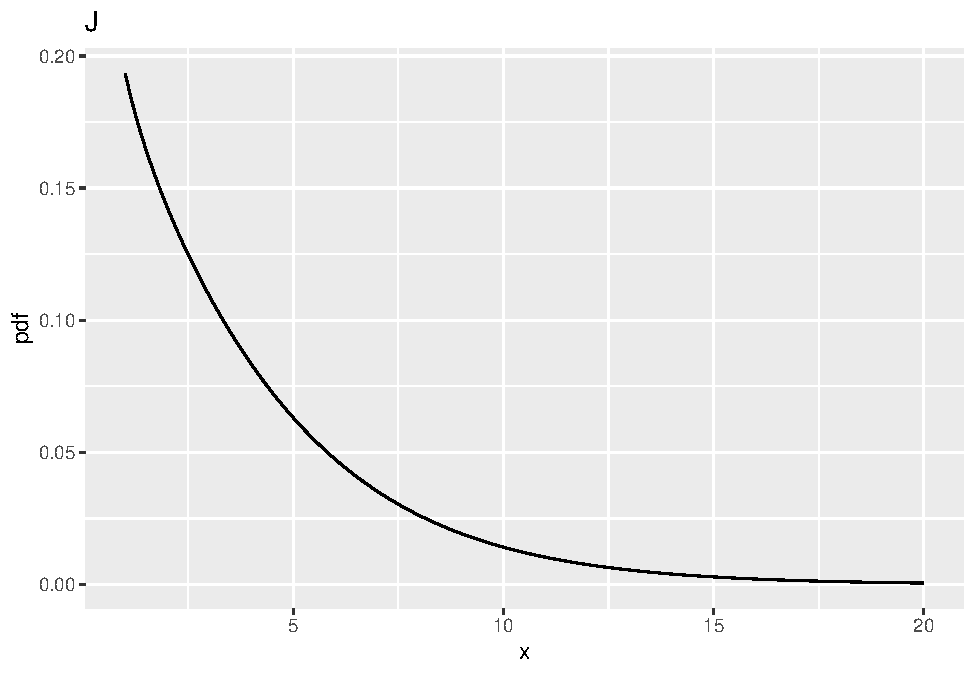
\includegraphics{19a-fdistribution_files/figure-latex/unnamed-chunk-5-2.pdf} 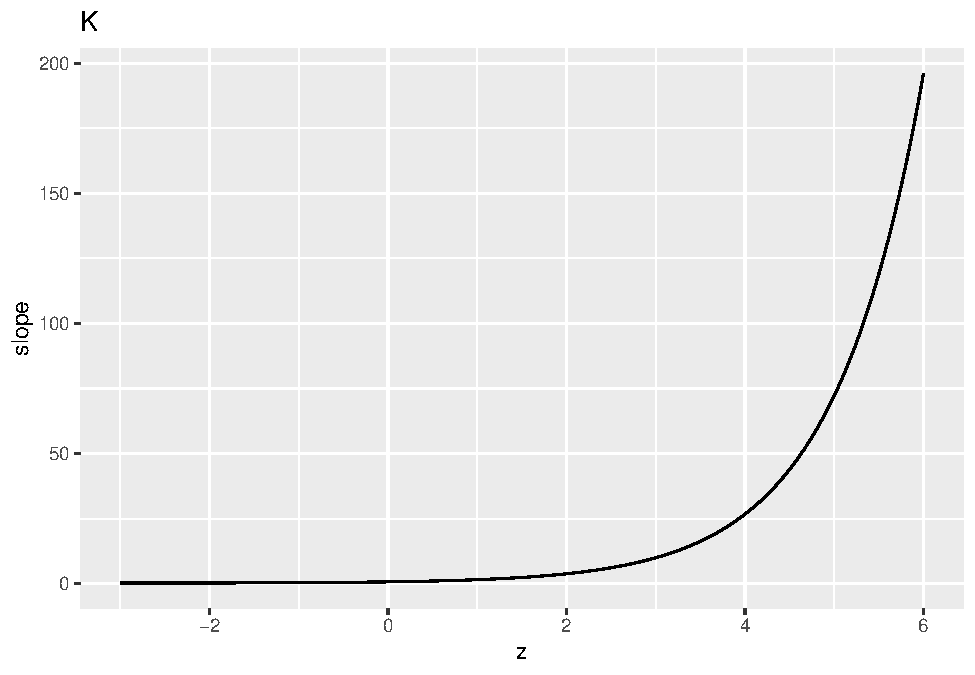
\includegraphics{19a-fdistribution_files/figure-latex/unnamed-chunk-5-3.pdf} 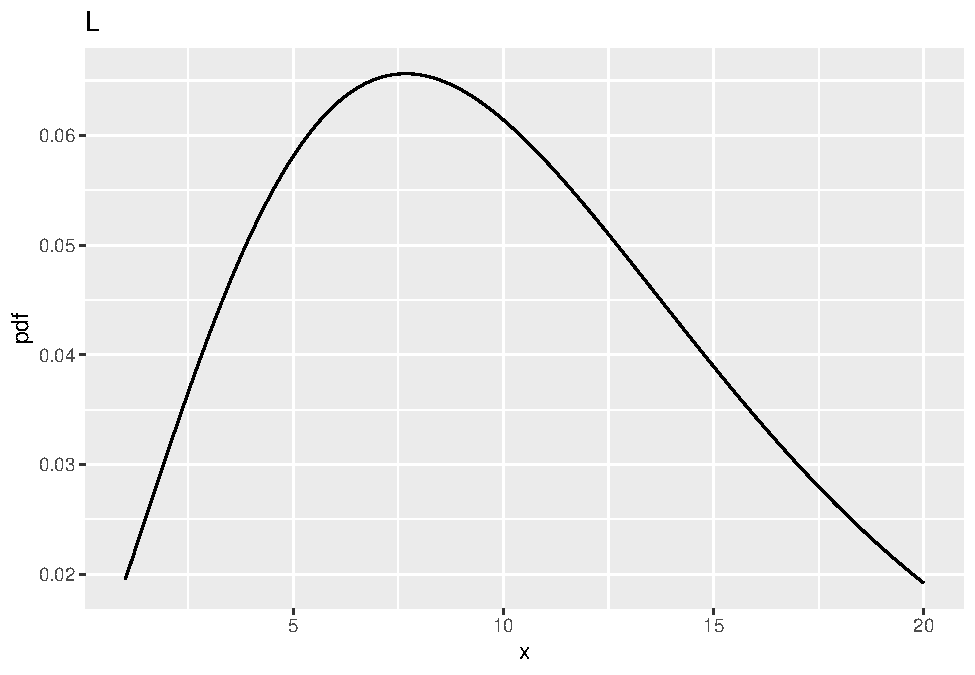
\includegraphics{19a-fdistribution_files/figure-latex/unnamed-chunk-5-4.pdf}

\begin{tabular}{l|r|r|r|r|r}
\hline
  & ndf & ddf & fCrit & ncp & pFgtFCrit\\
\hline
A & 2 & 10 & 4.102821 & 0 & 0.0500000\\
\hline
B & 2 & 10 & 4.102821 & 2 & 0.1775840\\
\hline
C & 2 & 10 & 4.102821 & 5 & 0.3876841\\
\hline
D & 2 & 10 & 4.102821 & 10 & 0.6769776\\
\hline
E & 2 & 100 & 3.087296 & 0 & 0.0500000\\
\hline
F & 2 & 100 & 3.087296 & 2 & 0.2199264\\
\hline
G & 2 & 100 & 3.087296 & 5 & 0.4910802\\
\hline
H & 2 & 100 & 3.087296 & 10 & 0.8029764\\
\hline
I & 1 & 100 & 3.936143 & 0 & 0.0500000\\
\hline
J & 1 & 100 & 3.936143 & 2 & 0.2883607\\
\hline
K & 1 & 100 & 3.936143 & 5 & 0.6004962\\
\hline
L & 1 & 100 & 3.936143 & 10 & 0.8793619\\
\hline
\end{tabular}

\hypertarget{comments-2}{%
\section{Comments}\label{comments-2}}

\begin{itemize}
\tightlist
\item
  All comparisons in this sections are at the same values of \texttt{ncp} defined above and at \texttt{ddf} = 100.
\item
  And between \texttt{ndf} = 1 and \texttt{ndf} = 2.
\end{itemize}

\hypertarget{fig.-i}{%
\subsection{Fig. I}\label{fig.-i}}

\begin{itemize}
\tightlist
\item
  This corresponds to \texttt{ncp} = 0, \texttt{ndf} = 1 and \texttt{ddf} = 100.
\item
  The critical value is \texttt{fCrit\_1\_100} = 3.936143.
\item
  Notice the increase in the critical value as compared to the corresponding value for \texttt{ndf\ =\ 2}, i.e., 3.0872959.
\item
  One expects power to decrease: the following code demonstrates that as \texttt{ndf} increases, the critical value \texttt{fCrit} decreases.
\item
  In significance testing generally \texttt{ndf} = I -1.
\item
  It more likely that the NH will be rejected with increasing numbers of treatments.
\end{itemize}

\begin{tabular}{r|r|r}
\hline
ndf & ddf & fCrit\\
\hline
1 & 100 & 3.936143\\
\hline
2 & 100 & 3.087296\\
\hline
5 & 100 & 2.305318\\
\hline
10 & 100 & 1.926692\\
\hline
12 & 100 & 1.850255\\
\hline
15 & 100 & 1.767530\\
\hline
20 & 100 & 1.676434\\
\hline
\end{tabular}

\hypertarget{fig.-j}{%
\subsection{Fig. J}\label{fig.-j}}

\begin{itemize}
\tightlist
\item
  This corresponds to \texttt{ncp} = 2, \texttt{ndf} = 1 and \texttt{ddf} = 100.
\item
  Now \texttt{prob\ \textgreater{}\ fCrit\_1\_100} = 0.2883607, 0.1351602, 0.0168844, \ensuremath{8.9992114\times 10^{-4}}, \ensuremath{3.2584757\times 10^{-4}}, \ensuremath{8.1619807\times 10^{-5}}, \ensuremath{1.1084132\times 10^{-5}}, larger than the previous value 0.2199264.
\item
  The power has actually increased.
\end{itemize}

\hypertarget{fig.-k}{%
\subsection{Fig. K}\label{fig.-k}}

\begin{itemize}
\tightlist
\item
  This corresponds to \texttt{ncp} = 5, \texttt{ndf} = 1 and \texttt{ddf} = 100`',
\item
  Now \texttt{prob\ \textgreater{}\ fCrit\_1\_100} = 0.6004962, 0.3632847, 0.0699798, 0.0048836, 0.0018367, \ensuremath{4.6889533\times 10^{-4}}, \ensuremath{6.2058692\times 10^{-5}}, larger than the previous value 0.4910802.
\item
  Again, the power has actually increased.
\end{itemize}

\hypertarget{fig.-l}{%
\subsection{Fig. L}\label{fig.-l}}

\begin{itemize}
\tightlist
\item
  This corresponds to \texttt{ncp} = 10, \texttt{ndf} = 1 and \texttt{ddf} = 100
\item
  Now \texttt{prob\ \textgreater{}\ fCrit\_1\_100} is 0.8793619, 0.7000168, 0.2459501, 0.0290856, 0.0123033, 0.0035298, \ensuremath{5.1213398\times 10^{-4}}, larger than the previous value 0.8029764.
\item
  The power has actually increased.
\end{itemize}

\hypertarget{summary-1}{%
\section{Summary}\label{summary-1}}

\begin{itemize}
\tightlist
\item
  Power increases with increasing \texttt{ddf} and \texttt{ncp}.
\item
  The effect of increasing \texttt{ncp} is quite dramatic. This is because power depends on the square of \texttt{ncp}.
\item
  As \texttt{ndf} increases, \texttt{fCrit} decreases, which makes it more likely that the NH will be rejected.
\item
  With increasing numbers of treatments the probability is greater that the F-statistic will be large enough to exceed the critical value.
\end{itemize}

\hypertarget{references}{%
\section{References}\label{references}}

\hypertarget{rsm-operating-characteristics}{%
\chapter{RSM operating characteristics}\label{rsm-operating-characteristics}}

\hypertarget{rsm-operating-characteristics-how-much-finished}{%
\section{TBA How much finished}\label{rsm-operating-characteristics-how-much-finished}}

10\%

\hypertarget{introduction-2}{%
\section{Introduction}\label{introduction-2}}

\begin{itemize}
\tightlist
\item
  The purpose of this vignette is to explain the operating characteristics predicted by the RSM. It relates to Chapter 17 in my book \citep{chakraborty2017observer}.
\item
  This vignette is under development \ldots{}
\item
  Also to explain the difference between \texttt{dataset} members (\texttt{lesionID}, \texttt{lesionWeight}) and RSM parameters (\texttt{lesDistr}, \texttt{lesWghtDistr}).
\end{itemize}

\hypertarget{the-distinction-between-predicted-curves-and-empirical-curves}{%
\section{The distinction between predicted curves and empirical curves}\label{the-distinction-between-predicted-curves-and-empirical-curves}}

\begin{itemize}
\tightlist
\item
  Operating characteristics predicted by a model have zero sampling variability.\\
\item
  Empirical operating characteristics, which apply to datasets, have non-zero sampling variability.
\item
  If the model is correct, as the numbers of cases in the dataset increases, the empirical operating characteristic asymptotically approaches the predicted curve.
\end{itemize}

\hypertarget{the-rsm-model}{%
\section{The RSM model}\label{the-rsm-model}}

\begin{itemize}
\tightlist
\item
  The 3 RSM parameters and two additional parameters characterizing the dataset determine the wAFROC curve.
\item
  The 3 RSM parameters are \(\mu\), \(\lambda\) and \(\nu\).
\item
  The two dataset parameters are:

  \begin{itemize}
  \tightlist
  \item
    The distribution of number of lesions per diseased case, \texttt{lesDistr}.
  \item
    The distribution of lesion weights, \texttt{lesWghtDistr}.
  \end{itemize}
\item
  These parameters do not apply to individual cases; rather they refer to a large population (asymptotically infinite in size) of cases.
\end{itemize}

\begin{Shaded}
\begin{Highlighting}[]
\KeywordTok{str}\NormalTok{(dataset04}\OperatorTok{$}\NormalTok{lesions}\OperatorTok{$}\NormalTok{IDs)}
\CommentTok{#>  num [1:100, 1:3] 1 1 1 1 1 1 1 1 1 1 ...}
\KeywordTok{str}\NormalTok{(dataset04}\OperatorTok{$}\NormalTok{lesions}\OperatorTok{$}\NormalTok{weights)}
\CommentTok{#>  num [1:100, 1:3] 1 1 1 1 1 1 1 1 1 1 ...}
\end{Highlighting}
\end{Shaded}

\begin{itemize}
\tightlist
\item
  Note that the first index of both arrays is the case index for the 100 abnormal cases in this dataset.
\item
  With finite number of cases the empirical operating characteristic (or for that matter any fitted operating characteristic) will have sampling variability as in the following example.
\end{itemize}

\hypertarget{the-empirical-wafroc}{%
\section{The empirical wAFROC}\label{the-empirical-wafroc}}

\begin{Shaded}
\begin{Highlighting}[]
\NormalTok{p <-}\StringTok{ }\KeywordTok{PlotEmpiricalOperatingCharacteristics}\NormalTok{(dataset04, }\DataTypeTok{opChType =} \StringTok{"wAFROC"}\NormalTok{)}
\NormalTok{p}\OperatorTok{$}\NormalTok{Plot}
\end{Highlighting}
\end{Shaded}

\includegraphics{19b-rsm-operating-characteristics_files/figure-latex/unnamed-chunk-2-1.pdf}

\begin{itemize}
\tightlist
\item
  The piecewise linear nature of the plot, with sharp breaks, indicates that this is due to a finite dataset.
\item
  In contrast the following code shows a smooth plot, because it is a model \emph{predicted} plot.
\end{itemize}

\hypertarget{the-predicted-wafroc}{%
\section{The predicted wAFROC}\label{the-predicted-wafroc}}

\begin{Shaded}
\begin{Highlighting}[]
\CommentTok{## Following example is for mu = 2, lambda = 1, nu = 0.6. 20% of the diseased }
\CommentTok{## cases have a single lesion, 40% have two lesions, 10% have 3 lesions, }
\CommentTok{## and 30% have 4 lesions.  }
\NormalTok{lesDistr <-}\StringTok{ }\KeywordTok{c}\NormalTok{(}\FloatTok{0.2}\NormalTok{, }\FloatTok{0.4}\NormalTok{, }\FloatTok{0.1}\NormalTok{, }\FloatTok{0.3}\NormalTok{)}

\CommentTok{## On cases with one lesion the weights are 1, on cases with 2 lesions the weights}
\CommentTok{## are 0.4 and 0.6, on cases with three lesions the weights are 0.2, 0.3 and 0.5, and}
\CommentTok{## on cases with 4 lesions the weights are 0.3, 0.4, 0.2 and 0.1: }
\NormalTok{relWeights <-}\StringTok{ }\KeywordTok{c}\NormalTok{(}\FloatTok{0.3}\NormalTok{,  }\FloatTok{0.4}\NormalTok{, }\FloatTok{0.2}\NormalTok{,  }\FloatTok{0.1}\NormalTok{)}
\NormalTok{p <-}\StringTok{ }\KeywordTok{PlotRsmOperatingCharacteristics}\NormalTok{(}
  \DataTypeTok{mu =} \DecValTok{2}\NormalTok{, }
  \DataTypeTok{lambda =} \DecValTok{1}\NormalTok{, }
  \DataTypeTok{nu =} \FloatTok{0.6}\NormalTok{, }
  \DataTypeTok{OpChType =} \StringTok{"wAFROC"}\NormalTok{, }
  \DataTypeTok{lesDistr =}\NormalTok{ lesDistr, }
  \DataTypeTok{relWeights =}\NormalTok{ relWeights, }
  \DataTypeTok{legendPosition =} \StringTok{"bottom"}\NormalTok{, }\DataTypeTok{nlfRange =} \KeywordTok{c}\NormalTok{(}\DecValTok{0}\NormalTok{, }\DecValTok{1}\NormalTok{), }\DataTypeTok{llfRange =} \KeywordTok{c}\NormalTok{(}\DecValTok{0}\NormalTok{, }\DecValTok{1}\NormalTok{))}
\NormalTok{p}\OperatorTok{$}\NormalTok{wAFROCPlot}
\end{Highlighting}
\end{Shaded}

\includegraphics{19b-rsm-operating-characteristics_files/figure-latex/unnamed-chunk-3-1.pdf}

\hypertarget{the-distribution-of-number-of-lesions-and-weights}{%
\section{The distribution of number of lesions and weights}\label{the-distribution-of-number-of-lesions-and-weights}}

\begin{Shaded}
\begin{Highlighting}[]
\NormalTok{lesDistr}
\CommentTok{#> [1] 0.2 0.4 0.1 0.3}
\NormalTok{relWeights}
\CommentTok{#> [1] 0.3 0.4 0.2 0.1}
\end{Highlighting}
\end{Shaded}

\begin{itemize}
\tightlist
\item
  The \texttt{lesDistr} array 0.2, 0.4, 0.1, 0.3 specifies the fraction of diseased cases with the number of lesions corresponding to the column index. To specify a dataset with exactly 3 lesions per diseased case use \texttt{lesDist\ =\ c(0,\ 0,\ 1,\ 0)}.
\item
  The \texttt{relWeights} array 0.3, 0.4, 0.2, 0.1 specifies the relative weights.
\item
  For cases with 1 lesion, the weight is 1.
\item
  For cases with 2 lesions, the first lesion has weight 0.4285714 and the second lesion has weight 0.5714286, which are in the ratio 0.3 : 0.4 and sum to unity.
\item
  For cases with 3 lesions, the first lesion has weight 0.3333333, the second lesion has weight 0.4444444 and the third lesion has weight 0.2222222, which are in the ratio 0.3 : 0.4 : 0.2, and sum to unity.
\item
  For cases with 4 lesions, the weights are 0.3, 0.4, 0.2 and 0.1, which are in the ratio 0.3 : 0.4 : 0.2 : 0.1 and sum to unity.
\end{itemize}

\hypertarget{other-operating-characteristics}{%
\section{Other operating characteristics}\label{other-operating-characteristics}}

\begin{itemize}
\tightlist
\item
  By changing \texttt{OpChType} one can generate other operating characteristics.
\item
  Note that lesiion weights argument is not needed for ROC curves. It is only needed for \texttt{wAFROC} and \texttt{wAFROC1} curves.
\end{itemize}

\begin{Shaded}
\begin{Highlighting}[]
\NormalTok{lesDistr <-}\StringTok{ }\KeywordTok{c}\NormalTok{(}\FloatTok{0.2}\NormalTok{, }\FloatTok{0.4}\NormalTok{, }\FloatTok{0.1}\NormalTok{, }\FloatTok{0.3}\NormalTok{)}
\NormalTok{p <-}\StringTok{ }\KeywordTok{PlotRsmOperatingCharacteristics}\NormalTok{(}
  \DataTypeTok{mu =} \DecValTok{2}\NormalTok{, }
  \DataTypeTok{lambda =} \DecValTok{1}\NormalTok{, }
  \DataTypeTok{nu =} \FloatTok{0.6}\NormalTok{, }
  \DataTypeTok{OpChType =} \StringTok{"ROC"}\NormalTok{,}
  \DataTypeTok{lesDistr =}\NormalTok{ lesDistr,  }
  \DataTypeTok{legendPosition =} \StringTok{"bottom"}\NormalTok{)}
\NormalTok{p}\OperatorTok{$}\NormalTok{ROCPlot}
\end{Highlighting}
\end{Shaded}

\includegraphics{19b-rsm-operating-characteristics_files/figure-latex/unnamed-chunk-5-1.pdf}

\hypertarget{summary-2}{%
\section{Summary}\label{summary-2}}

\hypertarget{references-1}{%
\section{References}\label{references-1}}

\hypertarget{improper-rocs}{%
\chapter{Improper ROC curves}\label{improper-rocs}}

\hypertarget{improper-rocs-how-much-finished}{%
\section{TBA How much finished}\label{improper-rocs-how-much-finished}}

10\%

\hypertarget{the-binormal-model}{%
\section{The binormal model}\label{the-binormal-model}}

The binormal model has two parameters, \texttt{a} and \texttt{b}. The signal (or diseased cases) distribution has unit standard deviation.
The noise (or non-diseased cases) distribution has standard deviation \texttt{b}. The \texttt{a} parameter is the separation of the two distributions.

\hypertarget{improper-rocs-1}{%
\section{Improper ROCs}\label{improper-rocs-1}}

Binormal model fits invariably lead to ROC curves that inappropriately cross the chance diagonal, leading to a prediction of a region of the ROC curve where performance is worse than chance, even for expert observers. By convention, such curves are termed \emph{improper}. This vignette illustrates improper ROCs predicted by the binormal model.

\begin{Shaded}
\begin{Highlighting}[]
\NormalTok{  aArray <-}\StringTok{ }\KeywordTok{c}\NormalTok{(}\FloatTok{0.7}\NormalTok{, }\FloatTok{0.7}\NormalTok{, }\FloatTok{1.5}\NormalTok{, }\DecValTok{2}\NormalTok{)}
\NormalTok{  bArray <-}\StringTok{ }\KeywordTok{c}\NormalTok{(}\FloatTok{0.5}\NormalTok{, }\FloatTok{1.5}\NormalTok{, }\FloatTok{0.5}\NormalTok{, }\FloatTok{0.5}\NormalTok{)}
\NormalTok{  chance_diag <-}\StringTok{ }\KeywordTok{data.frame}\NormalTok{(}\DataTypeTok{x =} \KeywordTok{c}\NormalTok{(}\DecValTok{0}\NormalTok{,}\DecValTok{1}\NormalTok{), }\DataTypeTok{y =} \KeywordTok{c}\NormalTok{(}\DecValTok{0}\NormalTok{,}\DecValTok{1}\NormalTok{))}
\NormalTok{  p <-}\StringTok{ }\KeywordTok{PlotBinormalFit}\NormalTok{(aArray, bArray) }\OperatorTok{+}
\StringTok{    }\KeywordTok{scale_x_continuous}\NormalTok{(}\DataTypeTok{expand =} \KeywordTok{c}\NormalTok{(}\DecValTok{0}\NormalTok{, }\DecValTok{0}\NormalTok{)) }\OperatorTok{+}\StringTok{ }
\StringTok{    }\KeywordTok{scale_y_continuous}\NormalTok{(}\DataTypeTok{expand =} \KeywordTok{c}\NormalTok{(}\DecValTok{0}\NormalTok{, }\DecValTok{0}\NormalTok{)) }\OperatorTok{+}
\StringTok{    }\KeywordTok{theme}\NormalTok{(}\DataTypeTok{legend.position =} \KeywordTok{c}\NormalTok{(}\FloatTok{0.85}\NormalTok{, }\FloatTok{0.2}\NormalTok{))}
\NormalTok{p <-}\StringTok{ }\NormalTok{p }\OperatorTok{+}\StringTok{ }\KeywordTok{geom_line}\NormalTok{(}\DataTypeTok{data =}\NormalTok{ chance_diag, }\KeywordTok{aes}\NormalTok{(}\DataTypeTok{x =}\NormalTok{ x, }\DataTypeTok{y =}\NormalTok{ y), }\DataTypeTok{linetype=}\StringTok{"dotted"}\NormalTok{)}
\KeywordTok{print}\NormalTok{(p)}
\end{Highlighting}
\end{Shaded}

\begin{center}\includegraphics{19c-improper-rocs_files/figure-latex/unnamed-chunk-1-1} \end{center}

The red plot is the clearest example of an improper ROC. This type of curve occurs whenever \texttt{b\ \textless{}\ 1}. The chance line crossing near the upper right corner, around (0.919,0.919), and the fact that the ROC curve must eventually reach (1, 1) implies the curve must turn upwards as one approaches (1, 1), thereby displaying a ``hook''. Whenever \texttt{b\ !=\ 1} the hook is there, regardless of whether it is easily visible or not. If \texttt{b\ \textless{}\ 1} the hook is near the upper right corner. If \texttt{b\ \textgreater{}\ 1} the hook is near the origin (see green line, corresponding to \texttt{b\ =\ 1.5}). With increasing \texttt{a} the hook is less prominent (blue line corresponding to \texttt{a\ =\ 1.5,\ b\ =\ 0.5} and purple line corresponding to \texttt{a\ =\ 2,\ b\ =\ 0.5}). But it is there.

\hypertarget{reason-for-improper-rocs}{%
\section{Reason for improper ROCs}\label{reason-for-improper-rocs}}

The reason for the ``hook''" becomes apparent upon examination of the pdfs.
\includegraphics{19c-improper-rocs_files/figure-latex/unnamed-chunk-2-1.pdf} \includegraphics{19c-improper-rocs_files/figure-latex/unnamed-chunk-2-2.pdf}

\begin{verbatim}
#> a =  0.7 , b =  0.5
\end{verbatim}

Since \texttt{b\ \textless{}\ 1}, the diseased \emph{pdf} is broader and has a lower peak (since the integral under each distribution is unity) than the non-diseased pdf. Sliding an imaginary threshold to the left, starting from the extreme right, one sees that initially, just below \texttt{z\ =\ 7}, the diseased distribution starts being \emph{``picked up''} while the non-diseased distribution is not \emph{``picked up''}, causing the ROC to start with infinite slope near the origin (because TPF is increasing while FPF is not). Around \texttt{z\ =\ 2.5} the non-diseased distribution starts being \emph{``picked up''}, causing the ROC slope to decrease. Around \texttt{z\ =\ -3}, almost all of the non-diseased distribution has been \emph{``picked up''} which means FPF is near unity, but since not all of the broader diseased distribution has been \emph{``picked up''}, TPF is less than unity. Here is a region where \texttt{TPF\ \textless{}\ FPF}, meaning \emph{the operating point is below the chance diagonal}. As the threshold is lowered further, TPF continues to increase, as the rest of the diseased distribution is \emph{``picked up''} while FPF stays almost constant at unity. In this region, the ROC curve is approaching the upper right corner with almost infinite slope (because TPF is increasing but FPF is not).

\hypertarget{degenerate-rocs}{%
\chapter{Degenerate ROC curves}\label{degenerate-rocs}}

\hypertarget{two-helper-functions}{%
\section{Two helper functions}\label{two-helper-functions}}

\hypertarget{degenerate-datasets}{%
\section{Degenerate datasets}\label{degenerate-datasets}}

Metz defined binormal degenerate data sets as those that result in exact-fit binormal ROC curves of inappropriate shape consisting of a series of horizontal and/or vertical line segments in which the ROC ``curve'' crosses the chance line. The crossing of the chance line occurs because the degenerate data sets can be fitted exactly by infinite or zero values for the model slope parameter \texttt{b}, and infinite values for the decision thresholds, or both.

\hypertarget{understanding-degenerate-datasets}{%
\section{Understanding degenerate datasets}\label{understanding-degenerate-datasets}}

To understand this, consider that the non-diseased distribution is a Dirac delta function centered at zero (by definition such a function integrates to unity) and the unit variance diseased distribution is centered at 0.6744898. In other words this binormal model is characterized by \texttt{a\ =\ 0.6744898} and \texttt{b\ =\ 0}. What is the expected ROC curve? As the threshold \(\zeta\) is moved from the far right, gradually to the left, TPF will increase but FPF is stuck at zero until the threshold reaches zero. Just before reaching this point, the coordinates of the ROC operating point are (0, 0.75). The 0.75 is due to the fact that \texttt{z\ =\ 0} is -0.6744898 units relative to the center of the diseased distribution, so the area under the diseased distribution below \texttt{z\ =\ 0} is 0.25. Since \texttt{pnorm} is the probability \emph{below} the threshold, TPF must be its complement, namely 0.75. This explains the operating point (0,0.75), which lies on the y-axis. As the threshold crosses the zero-width delta function, FPF shoots up from 0 to 1, but TPF stays constant. Therefore, the operating point has jumped from (0, 0.75) to (1, 0.75). When the threshold is reduced further, the operating point moves up vertically, along the right side of the ROC plot, until the threshold is so small that virtually all of diseased distribution exceeds it and the operating point reaches (1, 1). The ROC curve is illustrated in plot A.

\begin{Shaded}
\begin{Highlighting}[]
\NormalTok{plotOP <-}\StringTok{ }\KeywordTok{data.frame}\NormalTok{(}\DataTypeTok{FPF =} \DecValTok{0}\NormalTok{, }\DataTypeTok{TPF =} \FloatTok{0.75}\NormalTok{)}
\NormalTok{a <-}\StringTok{ }\FloatTok{0.6744898}\NormalTok{; b <-}\StringTok{ }\DecValTok{0}
\NormalTok{plotCurve <-}\StringTok{ }\KeywordTok{BMPoints}\NormalTok{(a, b)}
\NormalTok{figA <-}\StringTok{ }\KeywordTok{ggplot}\NormalTok{(}\DataTypeTok{mapping =} \KeywordTok{aes}\NormalTok{(}\DataTypeTok{x =}\NormalTok{ FPF, }\DataTypeTok{y =}\NormalTok{ TPF)) }\OperatorTok{+}\StringTok{ }
\StringTok{  }\KeywordTok{geom_line}\NormalTok{(}\DataTypeTok{data =}\NormalTok{ plotCurve) }\OperatorTok{+}\StringTok{ }
\StringTok{  }\KeywordTok{geom_point}\NormalTok{(}\DataTypeTok{data =}\NormalTok{ plotOP)  }\OperatorTok{+}\StringTok{ }
\StringTok{  }\KeywordTok{scale_x_continuous}\NormalTok{(}\DataTypeTok{expand =} \KeywordTok{c}\NormalTok{(}\DecValTok{0}\NormalTok{, }\DecValTok{0}\NormalTok{)) }\OperatorTok{+}\StringTok{ }
\StringTok{  }\KeywordTok{scale_y_continuous}\NormalTok{(}\DataTypeTok{expand =} \KeywordTok{c}\NormalTok{(}\DecValTok{0}\NormalTok{, }\DecValTok{0}\NormalTok{)) }\OperatorTok{+}
\StringTok{  }\KeywordTok{ggtitle}\NormalTok{(}\StringTok{"A"}\NormalTok{)}
\KeywordTok{print}\NormalTok{(figA)}
\end{Highlighting}
\end{Shaded}

\begin{center}\includegraphics{19d-degenerate-rocs_files/figure-latex/unnamed-chunk-2-1} \end{center}

This is an extreme example of an ROC curve with a ``hook''. If the data is such that the only operating point provided by the observer is (0,0.75) then this curve will be an exact fit to the operating point.

\hypertarget{the-exact-fit-is-not-unique}{%
\section{The exact fit is not unique}\label{the-exact-fit-is-not-unique}}

Actually, given one operating point (0, 0.75) the preceding fit is not even unique. If the diseased distribution is shifted appropriately to the right of its previous position, and one can determine the necessary value of a, then the ROC curve will shoot upwards through the operating point (0, 0.75) to (0, 0.9), as in plot B, before proceeding horizontally to (1, 0.9) and then completing the curve to (1, 1). If the diseased distribution is shifted well to the right, i.e., a is very large, then the ROC curve will shoot upwards past the operating point, as in plot C, all the way to (0,1) before proceeding horizontally to (1, 1).

\begin{Shaded}
\begin{Highlighting}[]
\NormalTok{a <-}\StringTok{ }\FloatTok{1.281552}\NormalTok{; b <-}\StringTok{ }\DecValTok{0}
\NormalTok{plotCurve <-}\StringTok{ }\KeywordTok{BMPoints}\NormalTok{(a, b)}
\NormalTok{figB <-}\StringTok{ }\KeywordTok{ggplot}\NormalTok{(}\DataTypeTok{mapping =} \KeywordTok{aes}\NormalTok{(}\DataTypeTok{x =}\NormalTok{ FPF, }\DataTypeTok{y =}\NormalTok{ TPF)) }\OperatorTok{+}\StringTok{ }
\StringTok{  }\KeywordTok{geom_line}\NormalTok{(}\DataTypeTok{data =}\NormalTok{ plotCurve) }\OperatorTok{+}\StringTok{ }
\StringTok{  }\KeywordTok{geom_point}\NormalTok{(}\DataTypeTok{data =}\NormalTok{ plotOP)  }\OperatorTok{+}\StringTok{ }
\StringTok{  }\KeywordTok{scale_x_continuous}\NormalTok{(}\DataTypeTok{expand =} \KeywordTok{c}\NormalTok{(}\DecValTok{0}\NormalTok{, }\DecValTok{0}\NormalTok{)) }\OperatorTok{+}\StringTok{ }
\StringTok{  }\KeywordTok{scale_y_continuous}\NormalTok{(}\DataTypeTok{expand =} \KeywordTok{c}\NormalTok{(}\DecValTok{0}\NormalTok{, }\DecValTok{0}\NormalTok{)) }\OperatorTok{+}
\StringTok{  }\KeywordTok{ggtitle}\NormalTok{(}\StringTok{"B"}\NormalTok{)}

\NormalTok{a <-}\StringTok{ }\OtherTok{Inf}\NormalTok{; b <-}\StringTok{ }\DecValTok{0}
\NormalTok{plotCurve <-}\StringTok{ }\KeywordTok{BMPoints}\NormalTok{(a, b)}
\NormalTok{figC <-}\StringTok{ }\KeywordTok{ggplot}\NormalTok{(}\DataTypeTok{mapping =} \KeywordTok{aes}\NormalTok{(}\DataTypeTok{x =}\NormalTok{ FPF, }\DataTypeTok{y =}\NormalTok{ TPF)) }\OperatorTok{+}\StringTok{ }
\StringTok{  }\KeywordTok{geom_line}\NormalTok{(}\DataTypeTok{data =}\NormalTok{ plotCurve) }\OperatorTok{+}\StringTok{ }
\StringTok{  }\KeywordTok{geom_point}\NormalTok{(}\DataTypeTok{data =}\NormalTok{ plotOP)  }\OperatorTok{+}\StringTok{ }
\StringTok{  }\KeywordTok{scale_x_continuous}\NormalTok{(}\DataTypeTok{expand =} \KeywordTok{c}\NormalTok{(}\DecValTok{0}\NormalTok{, }\DecValTok{0}\NormalTok{)) }\OperatorTok{+}\StringTok{ }
\StringTok{  }\KeywordTok{scale_y_continuous}\NormalTok{(}\DataTypeTok{expand =} \KeywordTok{c}\NormalTok{(}\DecValTok{0}\NormalTok{, }\DecValTok{0}\NormalTok{)) }\OperatorTok{+}
\StringTok{  }\KeywordTok{ggtitle}\NormalTok{(}\StringTok{"C"}\NormalTok{)}
\KeywordTok{print}\NormalTok{(figB);}\KeywordTok{print}\NormalTok{(figC)}
\end{Highlighting}
\end{Shaded}

\includegraphics{19d-degenerate-rocs_files/figure-latex/unnamed-chunk-3-1.pdf} \includegraphics{19d-degenerate-rocs_files/figure-latex/unnamed-chunk-3-2.pdf}

All of these represent exact fits to the observed operating point, with \texttt{b\ =\ 0} and different values of \texttt{a}. Not one of them is reasonable.

\hypertarget{comments-on-degeneracy}{%
\section{Comments on degeneracy}\label{comments-on-degeneracy}}

Degeneracy occurs if the observer does not provide any interior operating points. So why worry about it? Perhaps one has a non-cooperating observer, who is not heeding the instructions to \emph{spread the ratings, use all the bins}. A simple example shows that the observer could if fact be cooperating fully and is still unable to provide any interior data points. Consider 100 diseased cases consisting of 75 easy cases and 25 difficult ones and 100 easy non-diseased cases. The observer is expected to rate the 75 easy diseased cases as \emph{fives}, the difficult ones as \emph{ones} and the 100 non-diseased cases are rated \emph{ones}. No amount of coaxing \emph{please, please spread your ratings} is going to convince this observer to rate with twos, threes and fours any of the 75 easy diseased cases. If the cases are obviously diseased, and that is what is meant by \emph{easy cases}, they are supposed to be rated fives: \emph{definitely diseased}. Forcing them to rate some of them as \emph{probably diseased} or \emph{possibly diseased} would be irrational and guilty of bending the reading paradigm to fit the convenience of the researcher (early in his research career, the author used to believe in the existence of non-cooperating observers, so Metz's advice to \emph{spread the ratings} did not seem unreasonable at that time).

\hypertarget{a-reasonable-fit-to-the-degenerate-dataset}{%
\section{A reasonable fit to the degenerate dataset}\label{a-reasonable-fit-to-the-degenerate-dataset}}

If the dataset yields a single operating point (0, 0.75), what is a reasonable ROC plot? There is a theorem that given an observed operating point, the line connecting that point to (1, 1) represents a lower bound on achievable performance by the observer. The observer using a guessing mechanism to classify the remaining cases achieves the lower bound. Here is an explanation of this theorem. Having rated the 75 easy diseased cases as fives, the observer is left with 25 diseased cases and 100 non-diseased cases, all of which appear definitely non-diseased to the observer. Suppose the observer randomly rates 20\% of the remaining cases as fours. This would pick up five of the actually diseased cases and 20 non-diseased ones. Therefore, the total number of diseased cases rated four or higher is 80, and the corresponding number of non-diseased cases is 20. The new operating point of the observer is (0.20, 0.80). Now, one has two operating points, the original one on the y-axis at (0, 0.75) and an interior point (0.20, 0.80). Next, instead of randomly rating 20\% of the remaining cases as fours, the observer rates 40\% of them as fours, then the interior point would have been (0.40, 0.85). The reader can appreciate that simply by increasing the fraction of remaining cases that are randomly rated fours, the observer can move the operating point along the straight line connecting (0, 0.75) and (1, 1), as in plot D. Since a guessing mechanism is being used, this must represent a lower bound on performance. The resulting ROC curve is proper and the net AUC = 0.875.

\begin{Shaded}
\begin{Highlighting}[]
\NormalTok{mu <-}\StringTok{ }\OtherTok{Inf}\NormalTok{; alpha <-}\StringTok{ }\FloatTok{0.75}
\NormalTok{plotCurve <-}\StringTok{ }\KeywordTok{CBMPoints}\NormalTok{(mu, alpha)}
\NormalTok{figD <-}\StringTok{ }\KeywordTok{ggplot}\NormalTok{(}\DataTypeTok{mapping =} \KeywordTok{aes}\NormalTok{(}\DataTypeTok{x =}\NormalTok{ FPF, }\DataTypeTok{y =}\NormalTok{ TPF)) }\OperatorTok{+}\StringTok{ }
\StringTok{  }\KeywordTok{geom_line}\NormalTok{(}\DataTypeTok{data =}\NormalTok{ plotCurve) }\OperatorTok{+}\StringTok{ }
\StringTok{  }\KeywordTok{geom_point}\NormalTok{(}\DataTypeTok{data =}\NormalTok{ plotOP)  }\OperatorTok{+}\StringTok{ }
\StringTok{  }\KeywordTok{scale_x_continuous}\NormalTok{(}\DataTypeTok{expand =} \KeywordTok{c}\NormalTok{(}\DecValTok{0}\NormalTok{, }\DecValTok{0}\NormalTok{)) }\OperatorTok{+}\StringTok{ }
\StringTok{  }\KeywordTok{scale_y_continuous}\NormalTok{(}\DataTypeTok{expand =} \KeywordTok{c}\NormalTok{(}\DecValTok{0}\NormalTok{, }\DecValTok{0}\NormalTok{)) }\OperatorTok{+}
\StringTok{  }\KeywordTok{ggtitle}\NormalTok{(}\StringTok{"D"}\NormalTok{)}
\KeywordTok{print}\NormalTok{(figD)}
\end{Highlighting}
\end{Shaded}

\begin{center}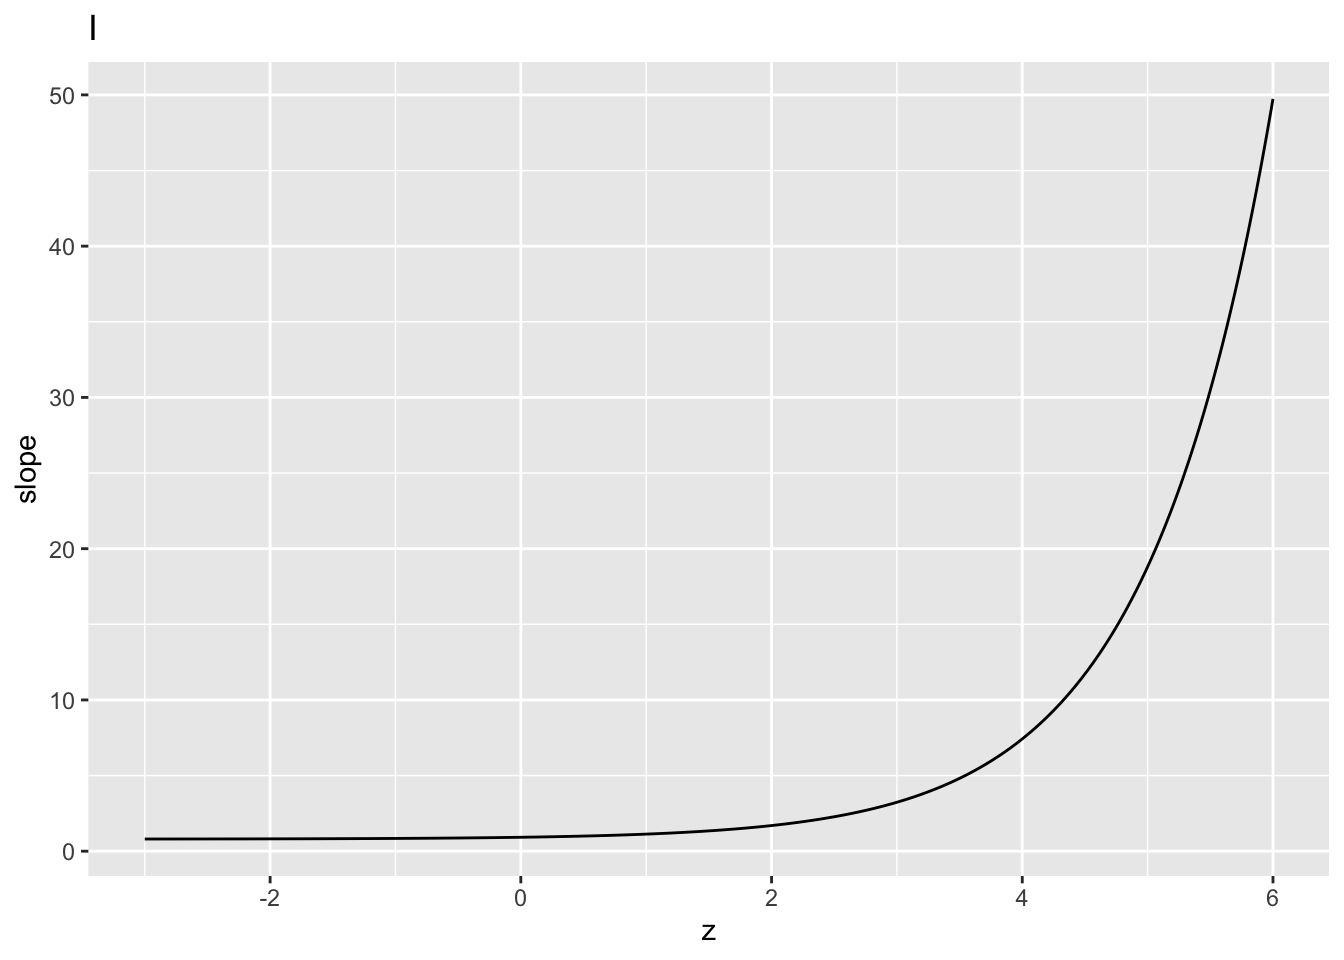
\includegraphics{19d-degenerate-rocs_files/figure-latex/unnamed-chunk-4-1} \end{center}

For this dataset this is in fact the fit yielded by the contaminated binormal model (CBM) and the radiological search model (RSM). Why should one select the lowest possible performance consistent with the data? Because it yields a \emph{unique} value for performance: any higher performance would not be unique.

\hypertarget{proproc-rocs}{%
\chapter{PROPROC ROC curves}\label{proproc-rocs}}

\hypertarget{helper-functions}{%
\section{Helper functions}\label{helper-functions}}

\hypertarget{definitions-of-proproc-parameters-in-terms-of-binormal-model-parameters}{%
\section{Definitions of PROPROC parameters in terms of binormal model parameters}\label{definitions-of-proproc-parameters-in-terms-of-binormal-model-parameters}}

\[c=\frac{b-1}{b+1};{{d}_{a}}=\frac{\sqrt{2}a}{\sqrt{1+{{b}^{2}}}}\]

\hypertarget{main-code-and-output}{%
\section{Main code and output}\label{main-code-and-output}}

\begin{Shaded}
\begin{Highlighting}[]
\NormalTok{c1Arr <-}\StringTok{   }\KeywordTok{c}\NormalTok{(}\OperatorTok{-}\FloatTok{0.1322804}\NormalTok{, }\FloatTok{0.2225588}\NormalTok{); daArr  <-}\StringTok{  }\KeywordTok{c}\NormalTok{(}\FloatTok{1.197239}\NormalTok{, }\FloatTok{1.740157}\NormalTok{)}
\NormalTok{myLabel <-}\StringTok{ }\KeywordTok{c}\NormalTok{(}\StringTok{"A"}\NormalTok{, }\StringTok{"B"}\NormalTok{, }\StringTok{"C"}\NormalTok{, }\StringTok{"D"}\NormalTok{)}
\NormalTok{myLabelIndx <-}\StringTok{ }\DecValTok{1}
\ControlFlowTok{for}\NormalTok{ (i }\ControlFlowTok{in} \DecValTok{1}\OperatorTok{:}\DecValTok{2}\NormalTok{)}
\NormalTok{\{}
\NormalTok{  c1 <-}\StringTok{ }\NormalTok{c1Arr[i]}
\NormalTok{  da <-}\StringTok{ }\NormalTok{daArr[i]}
\NormalTok{  ret <-}\StringTok{ }\KeywordTok{Transform2ab}\NormalTok{(da, c1)}
\NormalTok{  a <-}\StringTok{ }\NormalTok{ret}\OperatorTok{$}\NormalTok{a;b <-}\StringTok{ }\NormalTok{ret}\OperatorTok{$}\NormalTok{b}
  \ControlFlowTok{if}\NormalTok{ (i }\OperatorTok{==}\StringTok{ }\DecValTok{1}\NormalTok{) z <-}\StringTok{ }\KeywordTok{seq}\NormalTok{(}\OperatorTok{-}\DecValTok{3}\NormalTok{, }\DecValTok{0}\NormalTok{, }\DataTypeTok{by =} \FloatTok{0.01}\NormalTok{) }\CommentTok{# may need to adjust limits to view detail of slope plot}
  \ControlFlowTok{if}\NormalTok{ (i }\OperatorTok{==}\StringTok{ }\DecValTok{2}\NormalTok{) z <-}\StringTok{ }\KeywordTok{seq}\NormalTok{(}\OperatorTok{-}\DecValTok{3}\NormalTok{, }\DecValTok{5}\NormalTok{, }\DataTypeTok{by =} \FloatTok{0.01}\NormalTok{) }\CommentTok{# may need to adjust limits to view detail of slope plot}
  
\NormalTok{  FPF <-}\StringTok{ }\KeywordTok{seq}\NormalTok{(}\FloatTok{0.0}\NormalTok{, }\DecValTok{1}\NormalTok{, }\FloatTok{0.001}\NormalTok{)}
\NormalTok{  TPF <-}\StringTok{ }\KeywordTok{rocY}\NormalTok{(FPF, a, b)}
  
\NormalTok{  rocPlot <-}\StringTok{ }\KeywordTok{data.frame}\NormalTok{(}\DataTypeTok{FPF =}\NormalTok{ FPF, }\DataTypeTok{TPF =}\NormalTok{ TPF)}
\NormalTok{  plotRoc <-}\StringTok{ }\KeywordTok{ggplot}\NormalTok{(rocPlot, }\KeywordTok{aes}\NormalTok{(}\DataTypeTok{x =}\NormalTok{ FPF, }\DataTypeTok{y =}\NormalTok{ TPF)) }\OperatorTok{+}\StringTok{ }
\StringTok{    }\KeywordTok{geom_line}\NormalTok{()  }\OperatorTok{+}\StringTok{ }
\StringTok{   }\KeywordTok{scale_x_continuous}\NormalTok{(}\DataTypeTok{expand =} \KeywordTok{c}\NormalTok{(}\DecValTok{0}\NormalTok{, }\DecValTok{0}\NormalTok{)) }\OperatorTok{+}\StringTok{ }
\StringTok{    }\KeywordTok{scale_y_continuous}\NormalTok{(}\DataTypeTok{expand =} \KeywordTok{c}\NormalTok{(}\DecValTok{0}\NormalTok{, }\DecValTok{0}\NormalTok{))   }\OperatorTok{+}
\StringTok{    }\KeywordTok{ggtitle}\NormalTok{(myLabel[myLabelIndx]);myLabelIndx <-}\StringTok{ }\NormalTok{myLabelIndx }\OperatorTok{+}\StringTok{ }\DecValTok{1}

\NormalTok{  slope <-b}\OperatorTok{*}\KeywordTok{dnorm}\NormalTok{(a}\OperatorTok{-}\NormalTok{b}\OperatorTok{*}\NormalTok{z)}\OperatorTok{/}\KeywordTok{dnorm}\NormalTok{(}\OperatorTok{-}\NormalTok{z) }\CommentTok{# same as likelihood ratio}
  
\NormalTok{  slopePlot <-}\StringTok{ }\KeywordTok{data.frame}\NormalTok{(}\DataTypeTok{z =}\NormalTok{ z, }\DataTypeTok{slope =}\NormalTok{ slope)}
\NormalTok{  p <-}\StringTok{ }\KeywordTok{ggplot}\NormalTok{(slopePlot, }\KeywordTok{aes}\NormalTok{(}\DataTypeTok{x =}\NormalTok{ z, }\DataTypeTok{y =}\NormalTok{ slope)) }\OperatorTok{+}\StringTok{ }
\StringTok{    }\KeywordTok{geom_line}\NormalTok{()  }\OperatorTok{+}\StringTok{ }
\StringTok{    }\KeywordTok{scale_x_continuous}\NormalTok{(}\DataTypeTok{expand =} \KeywordTok{c}\NormalTok{(}\DecValTok{0}\NormalTok{, }\DecValTok{0}\NormalTok{)) }\OperatorTok{+}\StringTok{ }
\StringTok{    }\KeywordTok{scale_y_continuous}\NormalTok{(}\DataTypeTok{expand =} \KeywordTok{c}\NormalTok{(}\DecValTok{0}\NormalTok{, }\DecValTok{0}\NormalTok{))  }\OperatorTok{+}
\StringTok{    }\KeywordTok{ggtitle}\NormalTok{(myLabel[myLabelIndx]);myLabelIndx <-}\StringTok{ }\NormalTok{myLabelIndx }\OperatorTok{+}\StringTok{ }\DecValTok{1}
  \KeywordTok{print}\NormalTok{(plotRoc);}\KeywordTok{print}\NormalTok{(p)}
\NormalTok{\}}
\end{Highlighting}
\end{Shaded}

\includegraphics{19e-proproc-rocs_files/figure-latex/unnamed-chunk-2-1.pdf} \includegraphics{19e-proproc-rocs_files/figure-latex/unnamed-chunk-2-2.pdf} 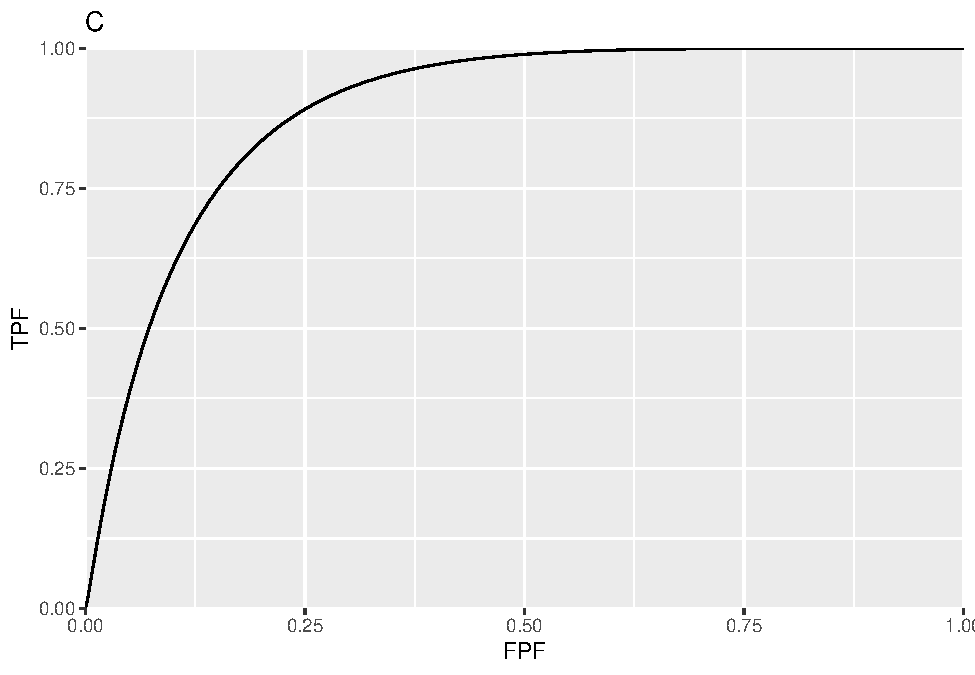
\includegraphics{19e-proproc-rocs_files/figure-latex/unnamed-chunk-2-3.pdf} \includegraphics{19e-proproc-rocs_files/figure-latex/unnamed-chunk-2-4.pdf}

\hypertarget{discussion}{%
\section{Discussion}\label{discussion}}

Plot A is for \texttt{c1} = -0.1322804, \texttt{da} = 1.197239 while plot C is for \texttt{c1} = 0.2225588, \texttt{da} = 1.740157. Plots B and D are the corresponding slope plots as functions of the binormal model z-sample. In plot A, the slope is infinite near the origin and the curve approaches the upper-right corner with finite slope. The situation is reversed in plot C where the slope is finite near the origin and the curve approaches the upper-right corner with zero slope.

These two readers are from a clinical dataset, \texttt{dataset01}. Highest rating inferred ROC data from original FROC data, were analyzed by PROPROC and the resulting parameter values are coded here. They were chosen as they demonstrate key differences in the shapes of proper ROC plots. Plot A corresponds to a negative value of \texttt{c1}, which implies \texttt{b\ \textless{}\ 1}. The slope of the proper ROC is infinite near the origin and approaches a positive constant near the upper right corner of the ROC. Plot C is for a positive value of \texttt{c1}, i.e., for \texttt{b\ \textgreater{}\ 1}. Now the slope of the proper ROC is finite near the origin and approaches zero near the upper right corner.

Considering plot D, as one ``cuts'' the slope axis horizontally with a sliding threshold, starting with very high values and moving downwards, the slope of the ROC curve starts at the origin with a large but finite value. This corresponds to the peak in plot D. Above the peak, there are no solutions for \texttt{z}. The slope decreases monotonically to zero, corresponding to the flattening out of the slope at zero for \texttt{z\ \textasciitilde{}\ \ -2}.

The two values of \texttt{z} corresponding to each cut implies, of course, that the binormal model based proper algorithm has to do a lot of bookkeeping, since each horizontal cut splits the decision axis into 3 regions. One can think of shrinking each of plots B \& D horizontally to zero width, and all that remains is the slope axis with a thick vertical line superimposed on it, corresponding to the horizontally collapsed curves. In plot B the vertical line extends from positive infinity down to about 0.1, and represents the range of decision variable samples encountered by the observer on the likelihood ratio scale. In plot D the vertical line extends from a finite value (\textasciitilde9.4) to zero. For the stated binormal model parameters values outside of these ranges are not possible.

\hypertarget{metz-eqn-36}{%
\chapter{Metz Eqn 36 numerical check}\label{metz-eqn-36}}

\hypertarget{helper-functions-1}{%
\section{Helper functions}\label{helper-functions-1}}

\hypertarget{main-code-and-output-1}{%
\section{Main code and output}\label{main-code-and-output-1}}

\begin{Shaded}
\begin{Highlighting}[]
\NormalTok{npts <-}\StringTok{  }\DecValTok{10000}
\ControlFlowTok{for}\NormalTok{ (i }\ControlFlowTok{in} \DecValTok{1}\OperatorTok{:}\DecValTok{2}\NormalTok{) \{}
  \ControlFlowTok{for}\NormalTok{ (j }\ControlFlowTok{in} \DecValTok{1}\OperatorTok{:}\DecValTok{5}\NormalTok{) \{}
\NormalTok{    C  <-}\StringTok{  }\NormalTok{c1[i,j]}
\NormalTok{    da  <-}\StringTok{  }\NormalTok{d_a1[i,j]}
\NormalTok{    ret <-}\StringTok{ }\KeywordTok{GetLimits}\NormalTok{(da,C)}
\NormalTok{    LL <-}\StringTok{ }\NormalTok{ret}\OperatorTok{$}\NormalTok{LL;UL <-}\StringTok{ }\NormalTok{ret}\OperatorTok{$}\NormalTok{UL}
\NormalTok{    vc  <-}\StringTok{  }\KeywordTok{seq}\NormalTok{ (LL, UL, }\DataTypeTok{length.out =}\NormalTok{ npts)}
\NormalTok{    TPF  <-}\StringTok{  }\KeywordTok{TruePositiveFraction}\NormalTok{ (vc, da, C)}
\NormalTok{    FPF <-}\StringTok{ }\KeywordTok{FalsePositiveFraction}\NormalTok{ (vc, da, C)}
\NormalTok{    FPF <-}\StringTok{ }\KeywordTok{rev}\NormalTok{(FPF);TPF <-}\StringTok{ }\KeywordTok{rev}\NormalTok{(TPF)}
\NormalTok{    df2 <-}\StringTok{ }\KeywordTok{data.frame}\NormalTok{(}\DataTypeTok{FPF =}\NormalTok{ FPF, }\DataTypeTok{TPF =}\NormalTok{ TPF)}
    \CommentTok{# do integral numerically}
\NormalTok{    numAuc <-}\StringTok{ }\KeywordTok{trapz}\NormalTok{(FPF, TPF)}
    \CommentTok{# Implement Eqn. 36 from Metz-Pan paper }
\NormalTok{    rho <-}\StringTok{ }\OperatorTok{-}\NormalTok{(}\DecValTok{1}\OperatorTok{-}\NormalTok{C}\OperatorTok{^}\DecValTok{2}\NormalTok{)}\OperatorTok{/}\NormalTok{(}\DecValTok{1}\OperatorTok{+}\NormalTok{C}\OperatorTok{^}\DecValTok{2}\NormalTok{);sigma <-}\StringTok{ }\KeywordTok{rbind}\NormalTok{(}\KeywordTok{c}\NormalTok{(}\DecValTok{1}\NormalTok{, rho), }\KeywordTok{c}\NormalTok{(rho, }\DecValTok{1}\NormalTok{))}
\NormalTok{    lower <-}\StringTok{ }\KeywordTok{rep}\NormalTok{(}\OperatorTok{-}\OtherTok{Inf}\NormalTok{,}\DecValTok{2}\NormalTok{);upper <-}\StringTok{ }\KeywordTok{c}\NormalTok{(}\OperatorTok{-}\NormalTok{da}\OperatorTok{/}\KeywordTok{sqrt}\NormalTok{(}\DecValTok{2}\NormalTok{),}\DecValTok{0}\NormalTok{)}
\NormalTok{    aucProproc <-}\StringTok{ }\KeywordTok{pnorm}\NormalTok{(da}\OperatorTok{/}\KeywordTok{sqrt}\NormalTok{(}\DecValTok{2}\NormalTok{)) }\OperatorTok{+}\StringTok{ }\DecValTok{2} \OperatorTok{*}\StringTok{ }\KeywordTok{pmvnorm}\NormalTok{(lower, upper, }\DataTypeTok{sigma =}\NormalTok{ sigma)}
\NormalTok{    aucProproc <-}\StringTok{  }\KeywordTok{as.numeric}\NormalTok{(aucProproc)}
    \KeywordTok{cat}\NormalTok{(}\StringTok{"i = "}\NormalTok{, i,}\StringTok{"j = "}\NormalTok{, j,}\StringTok{"C = "}\NormalTok{, C, }\StringTok{", da = "}\NormalTok{, da, }\StringTok{"aucProproc ="}\NormalTok{, aucProproc, }\StringTok{"Norm. Diff. = "}\NormalTok{, (aucProproc}\OperatorTok{-}\NormalTok{numAuc)}\OperatorTok{/}\NormalTok{aucProproc,}\StringTok{"}\CharTok{\textbackslash{}n}\StringTok{"}\NormalTok{)}
\NormalTok{  \}}
\NormalTok{\}}
\CommentTok{#> i =  1 j =  1 C =  -0.1322804 , da =  1.197239 aucProproc = 0.8014164 Norm. Diff. =  3.520017e-08 }
\CommentTok{#> i =  1 j =  2 C =  -0.08696513 , da =  1.771176 aucProproc = 0.8947898 Norm. Diff. =  4.741875e-08 }
\CommentTok{#> i =  1 j =  3 C =  -0.1444419 , da =  1.481935 aucProproc = 0.8526605 Norm. Diff. =  3.515431e-08 }
\CommentTok{#> i =  1 j =  4 C =  0.08046016 , da =  1.513757 aucProproc = 0.8577776 Norm. Diff. =  4.971428e-08 }
\CommentTok{#> i =  1 j =  5 C =  0.2225588 , da =  1.740157 aucProproc = 0.8909392 Norm. Diff. =  2.699855e-08 }
\CommentTok{#> i =  2 j =  1 C =  -0.08174248 , da =  0.6281251 aucProproc = 0.6716574 Norm. Diff. =  2.801793e-08 }
\CommentTok{#> i =  2 j =  2 C =  0.04976448 , da =  0.9738786 aucProproc = 0.7544739 Norm. Diff. =  5.275242e-08 }
\CommentTok{#> i =  2 j =  3 C =  -0.1326126 , da =  1.155871 aucProproc = 0.7931787 Norm. Diff. =  3.472577e-08 }
\CommentTok{#> i =  2 j =  4 C =  0.1182226 , da =  1.620176 aucProproc = 0.8740274 Norm. Diff. =  3.922161e-08 }
\CommentTok{#> i =  2 j =  5 C =  0.0781033 , da =  0.8928816 aucProproc = 0.7360989 Norm. Diff. =  3.798459e-08}
\end{Highlighting}
\end{Shaded}

\hypertarget{discussion-1}{%
\section{Discussion}\label{discussion-1}}

Note the close correspondence between the formula, Eqn. 36 in the Metz-Pan paper and the numerical estimate. As a historical note, Eqn. 31 and Eqn. 36 (they differ only in parameterizations) in the referenced publication are provided without proof -- it was probably obvious to Prof Metz or he wanted to leave it to us ``mere mortals'' to figure it out, as a final parting gesture of his legacy. The author once put a significant effort into proving it and even had a bright graduate student from the biostatistics department work on it to no avail. The author has observed that these equations always yield very close to the numerical estimates, to within numerical precisions, so the theorem is correct empirically, but he has been unable to prove it analytically. It is left as an exercise for a gifted reader to prove/disprove these equations.

  \bibliography{packages.bib,myRefs.bib}

\end{document}
